\documentclass[twoside,11pt,openright]{report}

\usepackage[latin1]{inputenc}
\usepackage[american]{babel}
\usepackage{a4}
\usepackage{latexsym}
\usepackage{amssymb}
\usepackage{amsmath}
\usepackage{epsfig}
\usepackage[T1]{fontenc}
\usepackage{lmodern}
\usepackage[labeled]{multibib}
\usepackage{color}
\usepackage{datetime}
\usepackage{epstopdf}
\usepackage{graphicx}
\usepackage{subcaption}
\usepackage{hyperref}
\usepackage{enumitem} %Used to make lists smaller
\usepackage{float}
\usepackage{placeins}
\usepackage[table]{xcolor}
\usepackage{todonotes}
\usepackage{menukeys}
\usepackage{longtable}

%\usepackage{amssymb}% http://ctan.org/pkg/amssymb
%\usepackage{pifont}% http://ctan.org/pkg/pifont

\newcommand{\x}{\scalebox{0.6}{x}}%
\newcommand{\m}{\scalebox{0.6}{(M)}}%
\renewcommand*\ttdefault{txtt}

%\newcommand{\todo}[1]{{\color[rgb]{.5,0,0}\textbf{$\blacktriangleright$#1$\blacktriangleleft$}}}

% \newcites{A,B}{Primary Bibliography,Secondary Bibliography}

% see http://imf.au.dk/system/latex/bog/

\begin{document}

%%%%%%%%%%%%%%%%%%%%%%%%%%%%%%%%%%%%%%%%%%%%%%%%%%%%%%%%%%%%%%%%%%%%%%%
	
\pagestyle{empty} 
\pagenumbering{roman} 
\vspace*{\fill}\noindent{\rule{\linewidth}{1mm}\\[4ex]
{\Huge\sf Wind Power and Electricity Price Forecasting Using Artificial Neural Networks to Support Decision Making in the Danish Electricity Market}\\[2ex]
{\huge\sf Brian Bak Laursen, 20071275}\\[2ex]
{\huge\sf Kristian Barrett, 20073457}\\[2ex]
\noindent\rule{\linewidth}{1mm}\\[4ex]	
\noindent{\Large\sf Master's Thesis, Department of Computer Science, ICT Product Development\\[1ex] 
\monthname\ \the\year  \\[1ex] Advisor: Niels Olof Bouvin\\[15ex]}\\[\fill]}

\epsfig{file=logo.eps}\clearpage


%%%%%%%%%%%%%%%%%%%%%%%%%%%%%%%%%%%%%%%%%%%%%%%%%%%%%%%%%%%%%%%%%%%%%%%

\pagestyle{plain}
\chapter*{Abstract}
\addcontentsline{toc}{chapter}{Abstract}
\definecolor{light-gray}{gray}{0.70}

\todo{in English\dots}

\chapter*{Resum\'e}
\addcontentsline{toc}{chapter}{Resum\'e}

\todo{in Danish\dots}

\chapter*{Acknowledgements}
\addcontentsline{toc}{chapter}{Acknowledgments}

\todo{\dots}

\vspace{2ex}
\begin{flushright}
  \emph{Brian Bak Laursen,}\\
  \emph{Aarhus, \today.}
\end{flushright}

\tableofcontents
\pagenumbering{arabic}
\setcounter{secnumdepth}{2}

%%%%%%%%%%%%%%%%%%%%%%%%%%%%%%%%%%%%%%%%%%%%%%%%%%%%%%%%%%%%%%%%%%%%%%%

\chapter{Introduction}
\label{ch:intro}
\section{The Problem}
Renewable energy has become increasingly important. Energy suppliers make it possible for their customers to choose between green and brown energy. Companies and persons promote themselves with green profiles to get a certain kind of image and it has become a choice of the individual company or home to be green. This is only one part of the picture, because the increased attention on green energy is influencing the market forces behind the scenes where acquisition of energy begins \cite{windPowerDanishLiberalized}. Various trading companies buy electricity on the deregulated energy market and since the amount of renewable energy in this market is increasing and will do for the years to come\cite{6, windPowerDanishLiberalized} the traders need to consider it carefully when buying and selling. The most essential task and basis for any decision making in the power market is to forecast the electricity price \cite{pjmForecast} and wind power production \cite{dayAheadImpactOfWindPowerForecasts}. Traditional producers can use the wind power predictions to strategically place their own energy in the market \cite{21}.
\\[0.5cm]
The electricity market consists of two instruments in order to facilitate trading between producers and consumers of energy: the pool which works as an online marketplace, and a framework to make physical contracts possible between both parties \cite{21}. The producers can make their electricity available and the consumers can bid correspondingly. An auction is made every hour to decide the market clearing price and which bids are accepted for that hour. The consumers and producers need to predict the hourly clearing prices to make plans for which bidding strategies to use. If a trader has a precise day-ahead prediction of the prices it will be easier to maximize profit by using the best possible strategy for exactly those conditions \cite{21}. The electricity traders will attempt to buy electricity in a low-price market and sell it when the price has come up like in other commodity markets \cite{FIND REF}. With a precise prediction they know when to buy and when to sell. 

Approximately 25\% of the total power production in Western Denmark was covered by wind power in 2008 and influenced the prices on the power market accordingly \cite{windPowerDanishLiberalized}. The impact on price is seen in wind power variations in areas where wind power production covers a substantial amount of the total supply which apply for Denmark. For this reason it cannot be avoided when predicting electricity prices\cite{dayAheadImpactOfWindPowerForecasts}. Since the amount of green energy in the entire Danish liberalized market is targeted to increase to 30\% by 2025 which is almost a doubling since 2008 \cite{windPowerDanishLiberalized} the influence will only become greater. The price impact from windmills will be even greater in strong wind periods and in areas with congestions in the power transmission capacity \cite{windPowerDanishLiberalized}. The increase in renewable energy makes the ability of predicting green energy production and the corresponding market price more vital. It is not trivial to predict wind production because green energy by nature is unpredictable, e.g. wind power is highly influenced by wind speed and air density. If the traders are able to predict wind power when doing actual price forecasts it will give rise to a huge advantage in the market when deciding to buy or sell \cite{dayAheadImpactOfWindPowerForecasts}. Price forecasting itself contains many other factors than wind power that needs to be considered equally \cite{21}.
\\[0.5cm] Traders buy and sell in real-time, intra-day or day-ahead \cite{FIND REF}. This puts constraints on a price prediction algorithm --- but what constraints depend solely on the type of trade. If the trader wishes to buy in real-time or hour-ahead the algorithm must perform and deliver a result within minutes or seconds. If it is day-ahead then the time-interval can be increased. This might result in a compromise on the margin of error because fast results make less time for analysis and computation. Another fact is that the closer you get to the time of the trade the more accurate the weather predictions will be which directly impacts the price prediction algorithm using it. The ability to make both short- and long-term forecasts is very important in the deregulated competitive electricity market because it helps the trader to reduce risks in terms of under/over estimating the revenues from potential sales and this of course also makes it easier to manage risk\cite{21}.
\\[0.5cm]
Demand has a huge influence on the electricity price. No demand, no electricity price, but if these were the only two variables to consider, a linear regression model could be used for establishing a relationship and thereby a prediction. Other dynamic elements have an impact on the price and therefore the linear regression approach would result in the presence of serial correlation in the error \cite{21}. For instance will overestimated energy prices for one year most likely lead to overestimates the next year since it does not account for all the dynamic parameters. It is necessary to carefully consider all variables and characteristics of the price that we are trying to predict in the electricity market and then use a model that handles correlated errors based on this. The most noticeable characteristics are \cite{21}:
\begin{itemize}
\item High frequency;
\item High volatility;
\item Unusual prices in times of very high demand;
\item Calendar effect (weekend, holidays);
\item Multiple seasonality (daily and weekly periodicity);
\end{itemize}
When doing electricity price forecasting these characteristics must be taken into consideration when modelling a prediction algorithm. 

\todo{describe how green decision making is important due to the regulation of prices if the consumption can be covered by the amount of green energy. This makes it important to identify the green energy.}
\section{Related Work}
This section will give an overview of concepts within the area of price and green energy prediction as well as decision support. The presented concepts will be elaborated as the thesis progress.
\subsection{Price Prediction Systems}
The stock price movements have similarities with electricity prices in terms of its non-linearity and chaotic/dynamic nature. Investors must take into account these factors when handling time series that are non-stationary, noisy and have structural breaks\cite{stockForecasting}. In addition, macro-economical elements significantly influence stock and electricity prices, e.g the economy in general, politics, bank rates and expectations of investors could be examples of such influences. In \cite{stockForecasting} they presented an Artificial Neural Network (ANN) approach to forecasting stock prices. These networks are powerful tools when solving complex problems because they possess qualities such as learning, generalizing, parallel processing and error endurance. The ANN in \cite{stockForecasting} is based on a Wavelet De-Noising-based Back Propagation (WDBP) that has the ability to filter away undesirable characteristics from the input. The purpose of the filtering is to separate stock price characteristics away from noise so that the prediction will have better chances of accuracy when all undesirable noise has been discarded. The prediction is then used by investors in their attempt to gain profits. 

A day-ahead forecasting algorithm that predicts electricity prices in the market based on Artificial Neural Network (ANN) and Similar Days Method (SDM) is described in \cite{pjmForecast}. The purpose is to give close estimates for several days to come. The estimates can be used by electricity traders in their decision making but also by transmission companies for different purposes. The companies can use it for scheduling a short-term generator outage in order to predict where it is most inexpensive. It can also be used by actual producers of energy to strategically bid into the market to increase prices. The price estimate itself plays a big role in decision making in all of these examples.

The combination of ANN and SDM is an attempt to simplify the ANN and make the prediction more accurate. The SDM technique averages five days that are similar to the corresponding forecast day. This makes the algorithm consider the influence of the most similar days and their price development compared to the day we wish to forecast. An actual forecast can be seen in figure ~\ref{fig:actualForecastMay13}.
\begin{figure}[!ht]
\centering
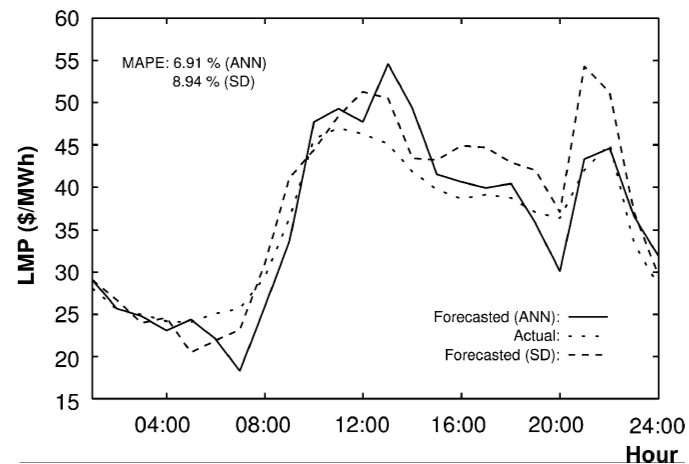
\includegraphics[width=0.8\linewidth,natwidth=898,natheight=587]{billeder/SDMANNAccuracy.png}
\caption{Actual day-ahead forecast from Saturday, May 13, 2006 \cite{pjmForecast}}
\label{fig:actualForecastMay13}
\end{figure}
The ANN is trained with 45 days from the day before the forecast, 45 days before and after the forecast day in the previous year.
\\[0.5cm]
Prediction algorithms are not only used by electricity traders but can also be a part of various applications. In \cite{22} they introduce an intelligent electricity broker (IEB) that is integrated into Smart Grids where it; 1) provides provision of en energy storage; 2) attempts to lower the electricity bill, and 3) optimally utilizes electricity during peak and low-peak energy production periods. The prediction algorithm is used by a decision algorithm to locate points in time where it is most feasible for the owner of the smart grid to either sell stored energy or buy energy if storage is low. It helps the system to lower the total amount of energy costs to the owner and also utilize the energy in the most intelligent way.
 

\subsection{Green Energy Production}
When dealing with prediction of green energy production it is necessary to look at the weather in more detail. Wind power prediction can be divided into two areas \cite{5}: 1) time-series analysis of power data and 2) wind speed prediction and conversion to power. What needs to be utilized in wind power prediction is wind speed and wind direction which of course has a big influence on how much energy a wind turbine generates. An approach to analysis and prediction of wind power generation is presented in \cite{WindPowerGenerationUsingANN} where an Artificial Neural Network is used to predict the production. The prediction is based on weather data such as wind speed, relative humidity but also for how many hours the windmill is generating power.

Another source of green energy is solar panels. Solar
prediction algorithms are very accurate when the weather conditions are steady but in changing weather a large error margin is seen. To predict power output from a solar farm the time-series prediction algorithms and Estimated Weighted Moving Average (EWMA) models can be used \cite{5}.

The prediction of wind power can be used en various contexts. Data centers is an example of a place where green energy prediction can be useful. It is often necessary for data centers to run long-running batch jobs where performance is measured in how many jobs it completes and the throughput. In \cite{5} they design an adaptive job scheduler that utilizes prediction of solar and wind energy production to scale workload. Earlier work has focused on using immediate available green energy and then cancelling and rescheduling jobs thereafter. The point in \cite{5} is instead to scale the number of jobs to the expected availability of green energy production by predicting it beforehand. This helps reducing the number of cancelled jobs as the jobs are then scheduled for whenever the energy is available. If the amount of green energy production is not sufficient for an immediate or emergency job the remainder will be covered by brown energy. The system reduces the amount of wasted green energy and increases the overall throughput of the data center.
\\[0.5cm]
In this thesis we will only be focusing on green energy that originates from windmills.


\subsection{Decision Support Systems}
Decision Support Systems (DSS) can help users in critical environments where careful situation assessment and decision making is necessary. This is valid for the financial markets such as the stock and electricity market where multiple dynamic factors are present \cite{UncertainInformation}.
\\[0.5cm]
A combination of an Artificial Neural Network approach, an eXtended Classifier System (XCS) and the idea of cooperative learning is presented in \cite{groupLearningDS}. It is an attempt to incorporate the best of all three in an intelligent financial decision support system. XCS and ANN are both forecasting technologies and the system compares their results in order to get the best price estimate. The cooperative learning element shows itself in the way a decision is made. Each agent selects the best investment strategy from their own point of view based on the price estimates. The agents can simulate several strategies in each session and select the potential of highest profit. This information is shared with the rest and the final investment decision is made based on the decision of the majority of the other agents in the system. The DSS archives investment strategies that showed to be profitable in a premium strategy library in order to collect the best strategies. The agents do not necessarily have to use the premium strategies but it makes sense to first try what have succeeded in the past and if that fails move on to a random selection strategy. 

The intelligent system described above makes all decisions for the agent as opposed to the HCI approach to DSS discussed in \cite{UncertainInformation}. The focus is on uncertain information and how to present it to the user in the best possible way. They argue that uncertain information cannot be denied and especially not in the domains with high risks such as the financial markets and military systems. The underlying reasoning algorithm used by the system will still make qualified estimates but the final decision is left to the user. The system will inform about uncertainties so the user can make trade-off's based on the information and then make a decision. Uncertainties can exist as different types such as bad data source reliability, conflict in data and data ambiguity but no matter the type it is presented to the user at all time. 

In \cite{UncertainInformation} is further discussed how to present information including linguistic, textual and graphical so that it is perceived better and faster by the user. Finally they present a number of guidelines that can used to develop a prototype of the interface for a DSS.

\section{The Method}
The available data are prices, wind productions and meteorological factors measured every hour from earlier years. When variables are observed sequentially over time it constitutes a time series where the values in the series evolve over time. Furthermore time series data are often strongly correlated over time which make it usable for prediction \cite[Chapter~7.1.2]{econometrics}. Based on the data and the non-linear nature of price forecasting and energy price prediction we want a system that is able to develop and learn from the past by analysing the time-series. Artificial Neural Networks can be categorized as Machine Learning \cite{18} and are networks that imitate the behaviour of the human brain \cite{1}. We choose to base our system on ANN because it gives us the power to be able to forecast energy prices based on how the prices have evolved in the past. Our decision is based on the nature of Artificial Neural Networks and how it is used in machine learning. It is often used in non-linear statistical analysis \cite{16} and has been used to predict various prices within the commodity market \cite{2,3,stockForecasting,pjmForecast}. We have chosen to use a multi-layered feed forward architecture since this is one of the most used and widely implemented in open-source frameworks \cite{17}.

We will base our work on Artificial Neural Networks and the Resilient Backpropagation (RPROP) algorithm used to train the network in order to predict electricity prices and wind power generation. The RPROP algorithm is a learning algorithm that uses weights to analyze the input dataset\cite{17} and it is a faster algorithm than its predecessor Backpropagation \cite{8,15}. It is commonly used on the feedforward architecture and is the most used and implemented algorithm on ANNs \cite{14,17}.
<<<<<<< .mineWe will base our work on Artificial Neural Networks and the resilient backpropagation (RPROP) algorithm used to train the network in order to predict electricity prices and wind power generation. It is faster than its predecessor Backpropagation \cite{8,15}.  The RPROP algorithm is a learning algorithm that uses weights to analyze the input dataset and to configure further learning \cite{17}. It is commonly used on the feedforward architecture and is the most used and implemented algorithm on ANNs \cite{14,17}. The historical data to include in the dataset will be identified through a systematic analysis of the electricity price and wind power characteristics together with experiments for verification. The result will be the optimal network settings for prediction of wind power and electricity prices in relation to best network structure, input, representation, size of training set and number of training epochs. The findings of our analysis and experimental results will be related to practical use in terms of decision making.=======We will base our work on Artificial Neural Networks and the Resilient Backpropagation (RPROP) algorithm used to train the network in order to predict electricity prices and wind power generation. The RPROP algorithm is a learning algorithm that uses weights to analyze the input dataset\cite{17} and it is a faster algorithm than its predecessor Backpropagation \cite{8,15}. It is commonly used on the feedforward architecture and is the most used and implemented algorithm on ANNs \cite{14,17}.

The prediction algorithm will be based on historical data which potentially could be a very large dataset. The more historical data included in the algorithm the more data needs to be processed. We need to analyse how much of this data is necessary for precise prediction and perhaps make tradeoffs to ensure performance for decision support.>>>>>>> .theirs

\section{The Hypothesis}
In this dissertation we take our outset in the growing need for green decision making. It is our intent to forecast green energy production and electricity prices within the electricity market by modelling an Artificial Neural Network using the back propagation algorithm for training of the network. The dataset for training consists of historical data that is relevant to the specific task. For instance when dealing with forecasting of wind power production for a wind farm, the most influential factors are meteorological such as wind speed, wind direction and air density together with historical production development of that particular farm. The energy prices are also influenced heavily by meteorological factors but it is instead combined with historical price development.
The goal is to investigate whether or not Back Propagation Artificial Neural Networks are a proper technology for doing prediction of green energy and electricity prices. Secondly, we are discussing the actual use of Artificial Neural Networks as Decision Support.
\\[0.5cm]
We will be focusing on; 1) modelling and implementing a working Back Propagation Artificial Neural Networks that are capable of predicting price and energy production within the electricity market; 2) evaluating predictions originating from Artificial Neural Networks in terms of both results and actual decision making.


%%%%%%%%%%%%%%%%%%%%%%%%%%%%%%%%%%%%%%%%%%%%%%%%%%%%%%%%%%%%%%%%%%%%%%%

\chapter{Main Concepts}
This chapter introduces and explains the technologies and concepts that are the foundation for the thesis.
\label{ch:foundations}
\section{Machine Learning}
Machine learning algorithms can figure out how to perform tasks by generalizing, where the goal is to generalize beyond the examples of a training set \cite{18}. The programs using the algorithm learn from data and as more data becomes available, more complex problems can be handled. Systems such as web search, spam filters and stock trading uses this approach.
\\[0.5cm]
Many learning algorithms exist and they are all based on combinations of three components \cite{18}; 1) the \textbf{representation} component makes an attempt to discover how to represent the input during training of the algorithm. What kind of information expressed in the data decides what representation algorithm to use; 2) the \textbf{evaluation} component has the objective of distinguishing between the best and the worst output from the representation component and let the next component decide which choice is the best. Basically it attempts to map the output to a specific value so that the next component can analyze it; 3) finally, the \textbf{optimization} component needs to search for the highest scoring output from the evaluation and then deliver it as a result. A greedy search could be an example of such a search (see figure ~\ref{fig:threeComponents}).
\begin{figure}[h!]
\centering
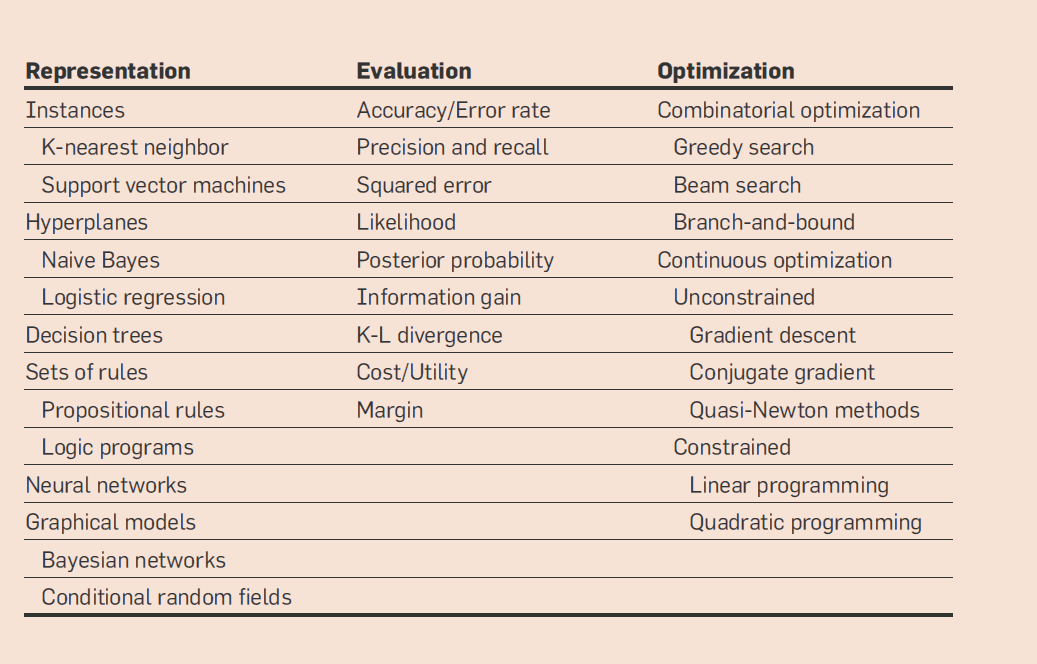
\includegraphics[width=0.6\linewidth,natwidth=898,natheight=587]{billeder/Table1-TheComponentsOfLearningAlgorithms.png}
\caption{The three components of learning algorithms \cite{18}}
\label{fig:threeComponents}
\end{figure}
\\[0.5cm] 
Machine learning cannot rely on data alone. Every learner must make assumptions beyond the data that is given to generalize beyond it \cite{18} because it is not possible to map the real world uniformly to a possible mathematical function. When meteorologists try to model the weather they make assumptions based on historical datasets that are similar to the current weather conditions. If enough historical occurrences resulted in the same weather condition the meteorologists must make the assumption that it can be classified as what have been seen before. The same is applicable when predicting electricity prices. We examine historical data and locate situations that are similar to the current and if enough examples with the same result is found it can be assumed that they are of the same type.
\\[0.5cm]
It can be the case that the system is not at all able to deliver a correct answer. This could result in the system guessing to the best of its ability or simply randoming an answer. This problem is called overfitting \cite{18}. Overfitting can be divided into bias and variance, where bias is when the learner consistently learns the same wrong thing over and over again. Variance is the learner's tendency to learn random things and ignoring the possibility of a more correct answer. See figure ~\ref{fig:biasandvariance} for an example with dart throwing.
\begin{figure}[h!]
\centering
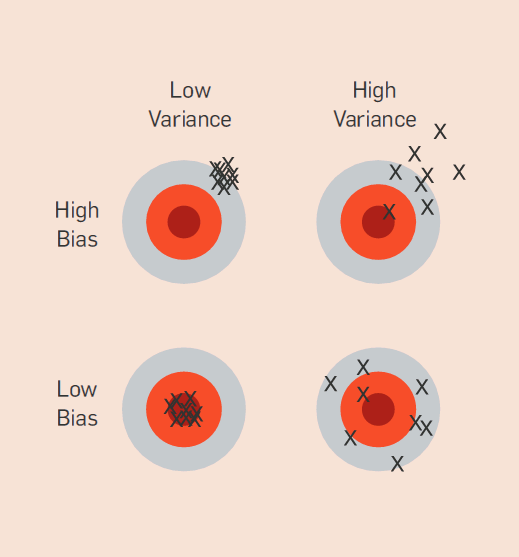
\includegraphics[width=0.5\linewidth,natwidth=898,natheight=587]{billeder/biasVSvariance.png}
\caption{Example of bias and variance in a dart throw \cite{18}}
\label{fig:biasandvariance}
\end{figure}

Machine learning is not only about the technical stuff but it also relies a great deal on intuition, creativity and  black art \cite{18}. 
\newline A way to achieve machine learning is by using a Artificial Neural Network. One way to model an ANN is to base it on the
Levenberg-Marquardt algorithm \cite{7,9,10}. It is a least squares algorithm that,
opposed to Backpropagation algorithm\cite{8}, is very fast at calculating the
results. It is a curve fitting algorithm mostly used on nonlinear problems with
a lot of unknowns[Need citation]. The algorithm can be used with Artificial Neural Networks and information approximation\cite{8} and it can be used in combination with the backpropagation algorithm to be used on a feedforward architecture of the neural network\cite{13}.

%%%%%%%%%%%%%%%%%%%%%%%%%%%%%%%%%%%%%%%%%%%%%%%%%%%%%%%%%%%%%%%%%%%%%%%
\newpage
\section{Artificial Neural Network}
\label{sec:annSection}
This section is based on information from the book AI techniques for game programming\cite{buckland2002ai} chapter 7, 8 \& 9. Also from the book Neural networks: a systematic introduction\cite{rojas1996neural} chapter 7.
\\[0.5cm]
Neural networks are models that imitate the brains behavior. They have been created as an option to model artificial intelligence and analyze machine learning. The human brain is made up of billions of neurons that are interconnected in a big grid. They communicate by firing electrical shocks through the network of neurons. The human brain is extremely complex and can calculate vast amounts of data in no time. This is why scientists and mathematicians have been trying to emulate this behavior to create artificial intelligence.

\begin{figure}[!ht]
\centering
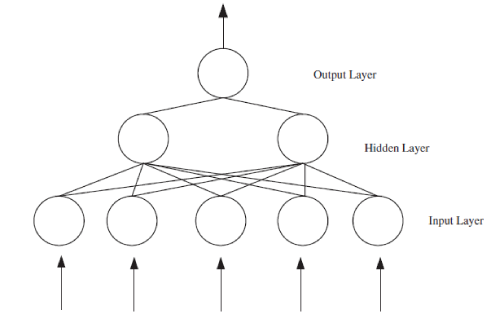
\includegraphics[width=0.8\linewidth,natwidth=898,natheight=587]{billeder/ANN.png}
\caption{A simple neural network with 3 layers. \cite{stockForecasting}}
\label{fig:ANN}
\end{figure}

Artificial neural networks (ANN) are artificial neurons (nodes) that are connected in a network. The network consists of an arbitrary number of layers that are interconnected. The most common structure in these networks are a feed forward structure. This kind of structure has the characteristic that it only flows data from the input layer through the layers to the output layer. There are no loops in the network thus making it unable to reiterate any information. Normally all of the nodes in the input layer is connected to all of the nodes in the second layer. The same connections are done in the next layers until we hit the output layer. This will give us the sum of all the previous nodes($x_i$) and their weights($w_i$)($\sum_{i=0}^{i=n+1} w_i x_i$) in every node in the next layer. See ~\ref{fig:weight_of_layers}.
\begin{figure}[!ht]
\centering
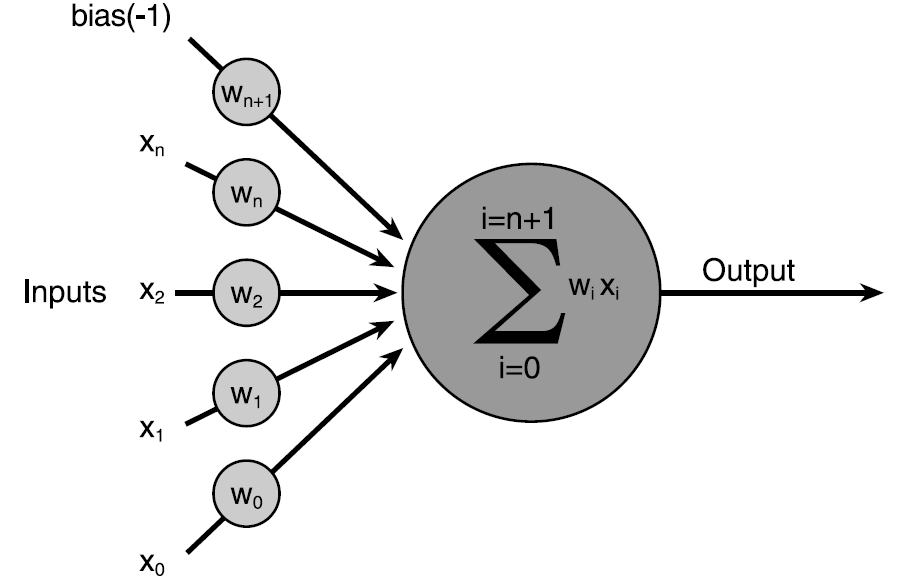
\includegraphics[width=0.8\linewidth,natwidth=898,natheight=587]{billeder/weight_of_layers.png}
\caption{How the weight is calculated from one layer to the next}
\label{fig:weight_of_layers}
\end{figure}
All of these connections carry a weight that dictates how data flows through the network and reflects the relations between the inputs and the outputs of the network. The inputs of the network should be all the factors that has an influence on the output we want from the network. In our example we would want to input; weather data, temperature, demand, availability \cite{21} to get the price as an output from the network.

Every node in our network contains an activation function. This function, when calculated, tells us whether the artificial neuron should fire or not. That is, if the neuron should transmit the data from the current layer to the next layer. There are a lot of different activation functions. The simplest form is the binary step function which either fires or it does not. This depends on the input and gives us a low threshold of complexity which is good in simple neural networks as the relations between the nodes do not need to be that fine grained. In more complex systems we want activation functions with a broader output range than binary. In many cases a sigmoid function is used as the activation function. This is because of the ''S''-shape which enables it to compute outputs in a non-linear way. The non-linear nature of the sigmoid functions is what makes the neural network able to compute non-trivial problems in reasonable sized networks. The sigmoid function allows the activation functions of the neurons to have a broader range of inputs which will produce an output compared to step activation functions. To be able to calculate a non-trivial problem in these kind of networks we need what is called a training algorithm. This algorithm depicts how the network evolves over time also known as learning. There are two kinds of learning; supervised learning and unsupervised learning.

\subsection{Unsupervised learning}
Unsupervised learning is when we do not have prior data to base our work on. Instead we have a problem where we want the neural network to try and estimate its behaviour relative to a specific task based on some assumptions we have about the system it performs on. It is commonly used with estimation problems like "Cluster Analysis", which in short is attempting to fit data into clusters of data that have some of the same criteria. This is often done by exploring the dataset and that is what unsupervised learning is good for. It also works with Artificial Intelligence(AI) that have to explore parts of the (virtual)world. In \cite{buckland2002ai} he explains how an unsupervised learning feed-forward artificial neural network trains itself using a genetic algorithm to keep track of the fitness function of the AI. The fitness function is used to tell the AI if it is doing good or doing bad and is used to train the network. It will get a plus score in the fitness function if it encounters what we are looking for and get negative if it hits something that we defined as "wrong". Based on this fitness function it will update the weights of the neural network accordingly to what is most beneficial for the network as a total. After it has been allowed to do a lot of runs it begins to get a sense of what it is exploring and should be able to make better choices for each run.

\subsection{Supervised learning}
Supervised learning are a set of algorithms that use a dataset which contains both the inputs and from those inputs what the output is expected to be. This dataset is used to train the neural network to make it able to do calculations on current data and predict the outcome. An example of an algorithm used for supervised learning is the back-propagation algorithm. 
It starts out by randomly assigning weights to all of the connections between the neurons. It then calculates the output of the network and compares it to the expected output. From that it calculates the error margin between the expected and the calculated output and adjusts the weights accordingly. This is done for all the hidden layers (as well) until we hit the input layer. All of these steps are called an epoch. We will repeat as many epochs as we need until the sum of all the errors are within a given threshold. The name of the algorithm originated from this approach where it propagates the error backwards in the network.

Supervised learning can be thought of as learning with a teacher. As an example we can use the XOR table:

\begin{table}[!ht]
\centering  % used for centering table
\begin{tabular}{c c c} % centered columns (3 columns)
Input \#1 & Input \#2 & Output \\ [0.5ex] % inserts table 
%heading
\hline                  % inserts single horizontal line
0 & 0 & 0  \\ % inserting body of the table
1 & 0 & 1  \\
0 & 1 & 1  \\
1 & 1 & 0 \\ [1ex] % [1ex] adds vertical space
\hline %inserts single line
\end{tabular}
\caption{This training set is very simple yet it illustrates a training set for a supervised learning algorithm very well.} % title of Table
\label{table:xor-table} % is used to refer this table in the text
\end{table}

In this dataset we have both of the inputs and we are given the expected output. This gives the back-propagation algorithm a direction to follow when minimizing the error function of the network. We can do this because we get an output that we can compare to the expected output which allows us to predict the direction that the error correction should take to come closer to the answer. Also the sigmoid activation function helps us closing in on the target output since the sigmoid function always has a positive derivative which ensures that we will always have a direction to follow\cite[p. 153]{rojas1996neural}. This is because the derivative of the sigmoid function always will point us towards the global minima of the expected function. If we take a look at ~\ref{table:xor-table} we are given inputs and outputs. We take the input 1 and 0 and we expect the output to be 1. The neural network will initialize weights and start to run the back-propagation. The back-propagation algorithm will compare the output it gets to the output we expected e.g. we may get an output of 0.5 (based on the random weight initialization) and this is compared to the expected output 1. Because of the sigmoid function we know what direction the weights should be corrected to come closer to the output of 1. This allows the back-propagation algorithm to recalculate the weights and be sure that it is heading for the global minima of the error function thus heading for the right output.
%[FORKLAR MATEMATIKKEN EVT MED EKSEMPEL s. 332 i bogen]

In neural networks bias neurons are often added to the layers to help them learn patterns. The bias neurons are added to give the activation functions the ability to change its output even if x is zero. If we look at the graph in figure ~\ref{fig:activationFunctions} it uses the following activation function: \begin{math} \frac{1}{(1+e^{(-cx)})} \end{math} where c is the weight.

\begin{figure}[!ht]
\centering
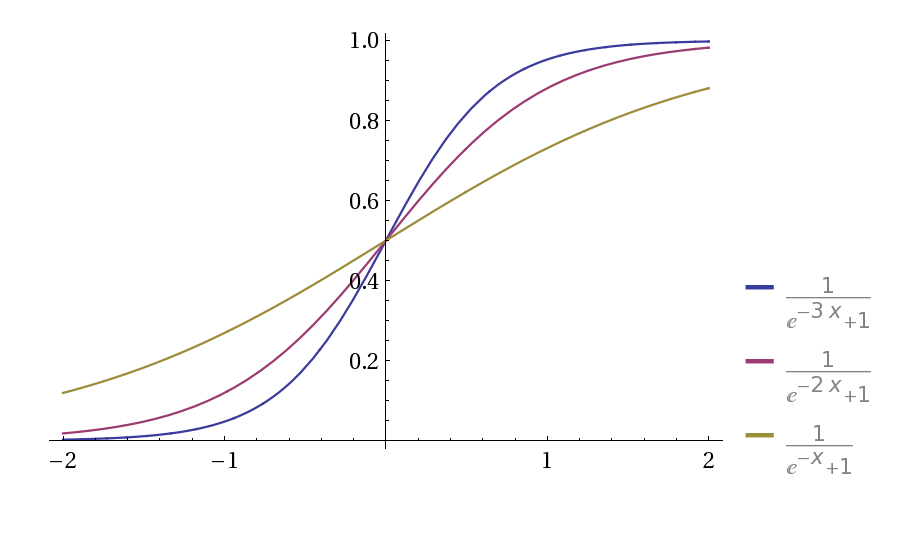
\includegraphics[width=0.8\textwidth ,natwidth=410,natheight=237]{billeder/ActivationFunctions.png}
\caption{}
\label{fig:activationFunctions}
\end{figure}

The figure shows how the gradient of the function alters with different weight values. Even though the gradient of the function is clearly altered by the weights the function is still outputting the same result for zero thus we cannot alter the output for x equal to zero just by altering the weights. This is what we use the bias for. If we apply a bias of one to all of the neurons we will be able to shift it either to the left or the right. In figure ~\ref{fig:activationFunctionsWithBias} we see the same function as before where the weight is set to 2. The difference is that we added a bias (b) to this function: \begin{math} \frac{1}{(1+e^{(-2x+b)})} \end{math} \cite[p. 165]{rojas1996neural} \cite{inductiveBias}

\begin{figure}[!ht]
\centering
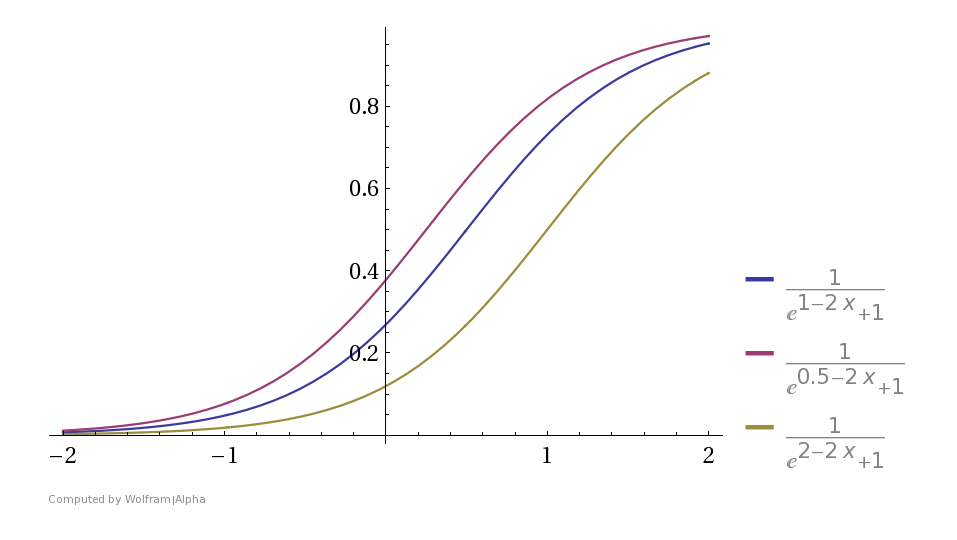
\includegraphics[width=0.8\textwidth ,natwidth=410,natheight=237]{billeder/ActivationFunctionsWithBias.png}
\caption{}
\label{fig:activationFunctionsWithBias}
\end{figure}

To calculate the error between input and output we use the mean squared error function. This function is given by: \begin{math} MSE=\frac{1}{n}\sum_{i=0}^{n}(\hat{y}_i-\bar{y}_i)^2 \end{math} where \begin{math} \hat{y}_i \end{math} is the ideal value and \begin{math} \bar{y}_i \end{math} is the actual value. We use this error calculation because it incorporates the bias \cite{meanSquaredError}

\subsection{Common pitfalls}
When we are trying to fit our algorithm and make it recognize patterns we will encounter several possible pitfalls. First of all there is the chance of ending up in a local minima. This is when the the back-propagation algorithm attempts to find the global minimum of the error curve, thus having reduce the error as much as possible. The algorithm works by trying to reduce this error margin a little step at a time. If it encounters a local minima on the curve and thinks it has reached the global minima it gets stuck and we will get inaccurate results ~\ref{fig:localMinimum}. 

\begin{figure}
\centering
\begin{minipage}{.5\textwidth}
  \centering
  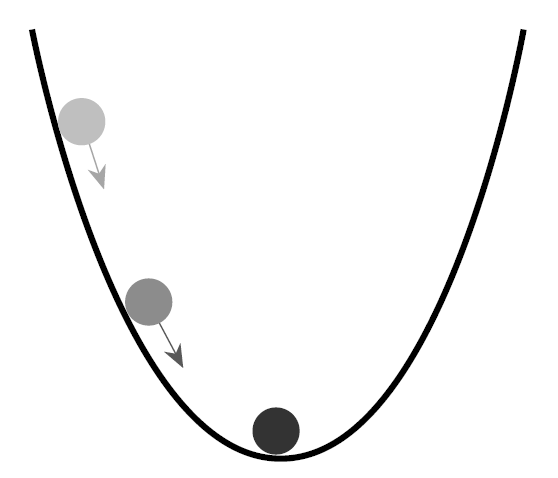
\includegraphics[width=.4\linewidth]{billeder/globalMinimum.png}
  \captionof{figure}{At the global minimum \cite[P. 318]{buckland2002ai}}
  \label{fig:globalMinimum}
\end{minipage}%
\begin{minipage}{.5\textwidth}
  \centering
  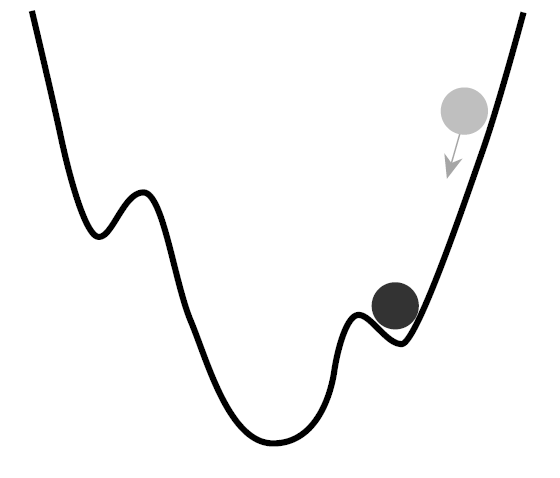
\includegraphics[width=.4\linewidth]{billeder/localMinimum.png}
  \captionof{figure}{Stuck in a local minimum \cite[P. 318]{buckland2002ai}}
  \label{fig:localMinimum}
\end{minipage}
\end{figure}

To avoid the backpropagation algorithm to falsely accept a local minima as the global minima we can give the algorithm momentum. This is done by adding a bit of the last error correction from the earlier layer to the next layers error correction. This way the algorithm, so to say, will scoot right by any small deviations in the error correction face.
\newline
Another pitfall when working with neural networks is over fitting the algorithm. This is when the algorithm instead of finding a generalized pattern in the inputs it will find an over-fit pattern that will fit exactly that input. This is better shown in figure ~\ref{fig:overfitting}.
\begin{figure}[!ht]
\centering
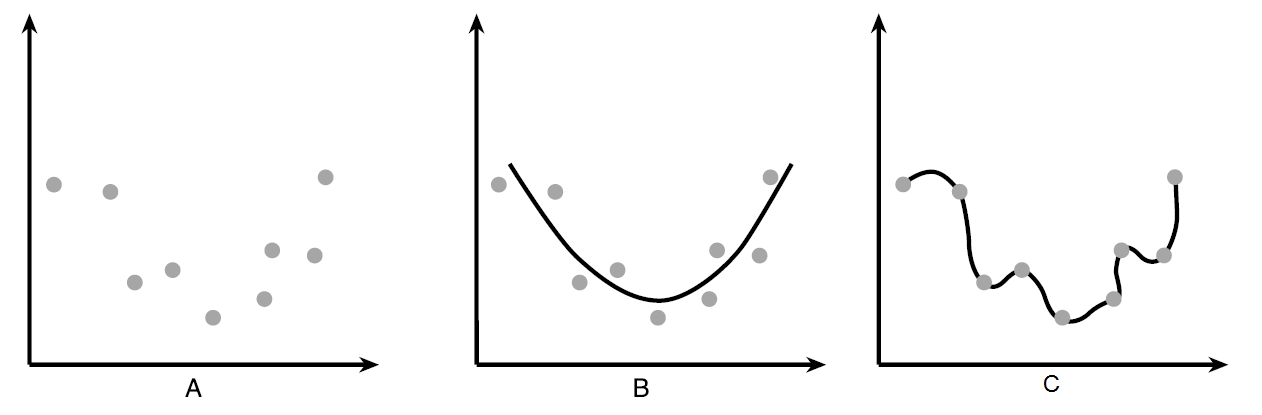
\includegraphics[width=0.8\linewidth,natwidth=1262,natheight=415]{billeder/overfitting.png}
\caption{A. The plot graph of the input B. The generalized function C. An over-fit function \cite[P. 319]{buckland2002ai}}
\label{fig:overfitting}
\end{figure}
This can be avoided by some simple techniques. First of all we want to reduce the neurons as much as possible as long as it does not interfere with our performance of the system. This is a trial and error problem and has to be tweaked along with evolving your neural network. We can add noise to avoid this problem. By adding noise(random data values) we prevent the algorithm from fitting the function to closely to the given data. Thus giving us a more generalized function where it hopefully will be able to fit new data presented to it better. Early stopping is another method to avoid over-fitting. This is only doable with large datasets where you can split it into two equal datasets. The first will work as a training set and the second will work as a validation set. We will keep training the dataset and checking with the validation set until the difference between those two start to increase.

\subsection{Summary}
This section touched the basics of neural networks and where the inspiration for these networks came from. It summed up what architecture we focus on in this paper namely the feed-forward architecture. This architecture allows data to only flow from input to output with no loops in it. We elaborated what activation functions are and how they are used in neural networks. In our neural network we are gonna use the more complex version called a sigmoid function which resembles and S if you draw it. This is done because it gives a wider variety of outputs than a normal step function. Since neural networks are all about the computer learning to calculate some very complex problem we need a learning algorithm. We explained that unsupervised learning algorithms are about exploring possibilities in a space and try to come close to a goal that we set up. It has no definitive goal (opposed to supervised learning) but a success factor that it tries to maximize. As mentioned we also talked about supervised learning and how these algorithms try to achieve the best possible result. This is done by trial-and-error where the algorithm learns until it satisfies an error margin we chose. Furthermore we talked about why and what bias is used for. It is a constant that is added to the calculations to prevent the algorithm to stall while trying to find the lowest error margin in our prediction. We also explained common pitfalls and how to avoid these. Among these were over-fitting of the function we are trying to a achieve which means it only fits the training set and not a general set of data. Also we talked about the algorithm falsely believing that the local minima was the global minima and therefore coming up with a wrong result.
We also talked about the training set and how this data is handled by the training algorithm. We mainly focus on supervised training since this is what we are gonna use in this thesis. A very important point to make here is that the training set is of utmost importance when it comes to performance and accuracy of our ANN. The training set has to be developed and refined during a training period of a network and relies a lot on experience and tinkering with the inputs. We need to normalize the input set so that it fits each other and all the parameters get the same weighting from the beginning. This is done not to favor any input unintentionally and vice versa. Also we can only have assumptions of on which form the inputs will give the best result and we might have to try different forms like numbers, bits, bitmaps etc. to get the best results. Also we might have a reason to think some data is important but that it turns out it just makes the calculations more complex without adding any nuance to the output and therefore can be omitted from the calculations.
All in all we tried to give a brief introduction to neural networks and the technologies that we use with it.

%%%%%%%%%%%%%%%%%%%%%%%%%%%%%%%%%%%%%%%%%%%%%%%%%%%%%%%%%%%%%%%%%%%%%%%
\newpage
\section{Prediction}
\label{sec:predictionSection}
Being able to predict electricity prices and green energy production is the basis for our thesis. Demand has a huge impact on the electricity price so this is also handled here. This section will introduce and give selected examples of these concepts within the different areas. 

\subsection{Electricity Demand}
\label{sec:ElectricityDemand}
Weather conditions have a impact on the electricity industry in terms of network infrastructure and electricity consumption. In \cite{19} they describe a multiple regression model that accurately predicts the monthly electricity demand based on weather and sociocultural conditions. The monthly electricity demand from this model shows a clear cyclic pattern which reflects the temperature changes during the year \cite{19}. Besides from weather conditions, social and economic factors also affect the monthly demand, e.g. the demand was decreased in Denmark during the \fnurl{financial crisis in 2009}{http://www.business.dk/investor/finanskrisen-saetter-elforbrug-i-bakgear}.

\subsubsection{Parametric multiple regression}
Parametric multiple regression is preferred in \cite{19} as opposed to an Artificial Neural Network used in this thesis. From a statistical error indices point of view they describe that the Artificial Neural Network (ANN) is a valid choice for prediction. The argument for multiple regression is the simplicity in adjusting input values for each analysis of electricity demand in the prediction model. 

To make a demand prediction based on weather conditions they have established a relationship between the two. To get an understanding of this relationship they have made a plot of the average monthly demand as a function of Central England Temperature (CET) \cite{19}. The plot (see figure ~\ref{fig:CET}) shows an inverse relationship where it can be seen that a lower temperature in general results in an increased load consumption. Winter gives rise to lighting and heating load which is consistent with lower temperatures, and conversely in the summer with temperatures above 18 degrees the consumption tends to increase again due to the need for cooling and air-condition \cite{19}.
\begin{figure}[h!]
\centering
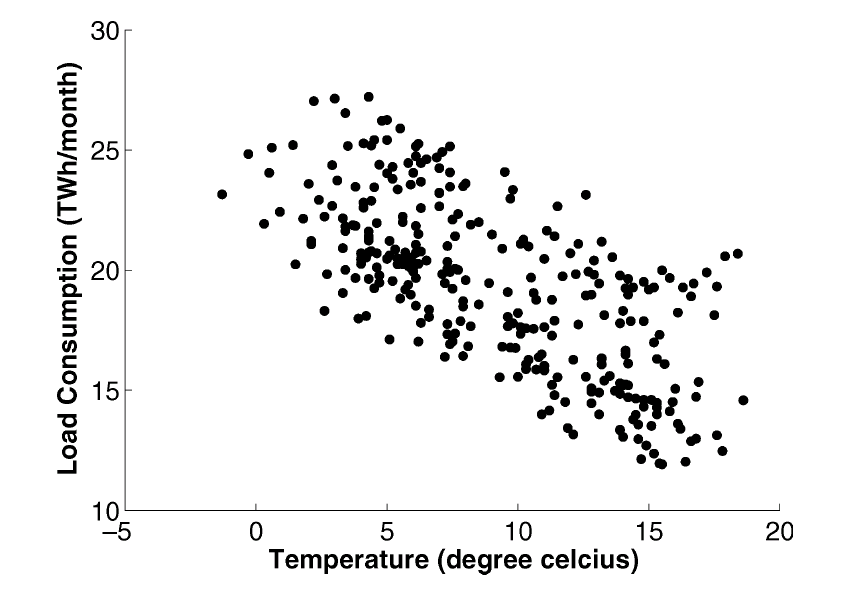
\includegraphics[width=0.8\linewidth,natwidth=898,natheight=587]{billeder/MeanMonthlyDemandEngland.png}
\caption{Function of monthly CET as a function from 1970 to 1995 \cite{19}}
\label{fig:CET}
\end{figure}

\subsubsection{Heating and Cooling Degree Days}
The nonlinear relationship between temperature and load consumption is turned into a concept called degree days. They introduce two categories of days; 1) Heating Degree Days (HDD) that is used to quantify when heating is required; 2) Cooling Degree Days (CDD) which is then used to quantify the need for cooling. The days are calculated from the CET data and give a more indicative picture than the temperature-load relationship \cite{19}. A simple explanation of the calculation follows.
\begin{center}
$CDD=\sum\limits_{d=1}^{N_{d}}(\gamma_{d})(T_{dm}-T_{base_{C}})$
\end{center} 
 
where $T_{base_{c}} = 20^{\circ}$ is the base temp and $T_{dm}$ is the mean daily temperature. $\gamma_{d} = 0$ if $T_{dm}-T_{base_{c}} < 0$ and $\gamma_{d} = 1$ if $T_{dm}-T_{base_{c}} > 0$. In other words if the temperature is above $20^{\circ}$ the day can be characterized as CDD and there is a need for cooling.
\begin{center}
$HDD=\sum\limits_{d=1}^{N_{d}}(1-\gamma_{d})(T_{base_{H}}-T_{dm})$
\end{center} 

where $T_{base_{h}} = 15.5^{\circ}$ is the base temp and again $T_{dm}$ is the mean daily temperature. $\gamma_{d} = 1$ if $T_{base_{h}}-T_{dm} < 0$ and $\gamma_{d} = 0$ if $T_{base_{h}}-T_{dm} > 0$. This means that on a day with temperatures below 15.5 degrees there is a need for heating. In both cases where $\gamma_{d} != 0$ a big difference has a greater impact on the demand.

Temperature is the most influential factor but other weather conditions can also be used when predicting the electricity demand, e.g. wind speed and rainfall can impact heating and lighting demand whereas direct sunshine can decrease the need for heating \cite{19}. The model can be expressed by the relation between all factors by adding them together, e.g. the HDD value automatically increase the total electricity demand if it is not zero and this apply to all other factors in the model seen below.

\begin{center} \^E$_{A}=\alpha_{0}+\alpha_{1}CDD+\alpha_{2}HDD+\alpha_{3}ELD
+\alpha_{4}V_{w}+\alpha_{5}M_{s}+\alpha_{6}M_{r}$ 
\end{center} 
 
Where $\alpha_{n}$ are constants, ELD is humidity, $V_{w}$ is wind speed, $M_{s}$ sunshine and $M_{r}$ rainfall.
The calculation model can also include socio-economic factors. Specifically the population growth has a natural impact on the electricity demand over time. The more people the higher the demand gets. This would give rise to an additional factor in the model considering the growth. The prediction model from \cite{19} comes within 3 percentage of the actual demand when it is run on data from 1996-2003 which they consider to be close (~\ref{fig:predicteddemand}).
\newline
\begin{figure}[h!]
\centering
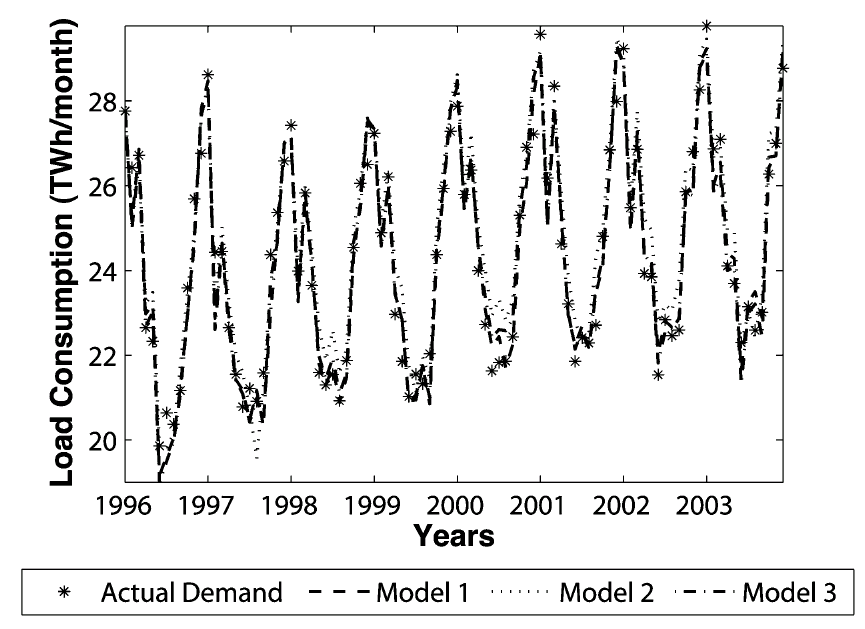
\includegraphics[width=0.8\linewidth,natwidth=898,natheight=587]{billeder/PredictionOfDemand.png}
\caption{The actual values and the predicted demand in a comparison \cite{19}}
\label{fig:predicteddemand}
\end{figure}

\subsubsection{Summary}
The electricity demand has great influence on the energy price. It is important to identify the influences of the demand because those inevitably also will have an affect on the electricity prices. 

The concept of Cooling Degree Days (CDD) and Heating Degree Days (HDD) has been described. They might give us an quantifiable parameter to measure the need for cooling and heating in Denmark. What it brings forward is the necessity for considering demand when predicting price and a potential of substituting demand with the parameters given --- wind speed, temperature, ect. The demand function (\^E$_{A}$) is presented. This function gives a picture of the factors that directly influence the demand and the possible mappings to our ANN as the demand part --- every parameter is an input.

\subsection{Wind Power Production}
The identification of rich wind resources have become important together with the increasing focus on green energy \cite{WindPowerGenerationUsingANN}. It is important to analyse and predict the wind power generation at a certain location before placing actual windmills. 
Wind speed, relative humidity and generation hours of the windmills are used as input for a Artificial Neural Network in \cite{WindPowerGenerationUsingANN}. It can come as no surprise that the meteorological factors like wind speed and air density have a huge impact on the wind power generation. Figure~\ref{fig:energyGeneration} shows how the monthly energy generation increases with the monthly average wind speed. 

\begin{figure}[h!]
\centering
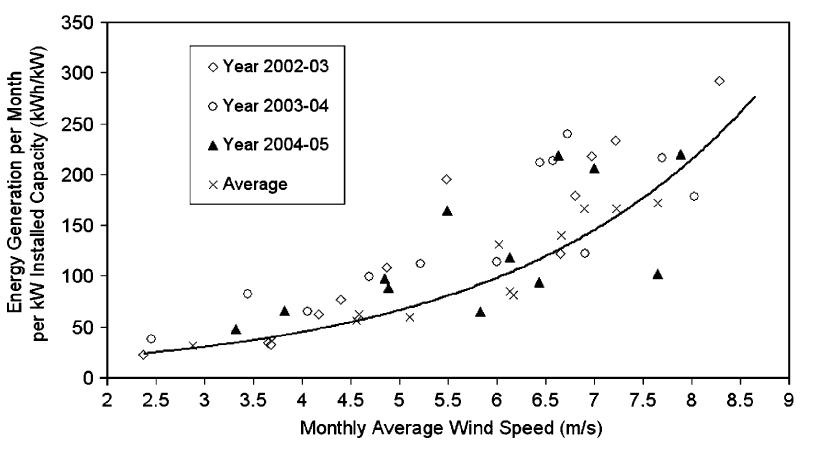
\includegraphics[width=0.8\linewidth,natwidth=898,natheight=587]{billeder/EnergyGenerationVsWindSpeed.png}
\caption{The influence of wind speed on the energy generation \cite{WindPowerGenerationUsingANN}}
\label{fig:energyGeneration}
\end{figure} 

The more "heavy" the air, the more energy is received by the windmill turbine. The humidity increases as as air density increases and because wind energy is proportional to air density the prediction algorithm needs humidity as input because it also accounts for temperature and pressure \cite{AirDensityInForecast}. Moist air is lighter than dry air because water molecules are less dense than the molecules in dry air such as oxygen and nitrogen. This basically means that the more air molecules like oxygen and nitrogen the more wind energy.

The last parameter in their prediction algorithm is generation hours which is the period in which the turbines produce power. The number of hours are influenced by f.x mechanical breakdowns, scheduled maintenance and low wind speeds. It is clear the the more generation hours the more energy is produced as seen in figure ~\ref{fig:energyGenerationFromHours}. The generation hours are hard to predict but can be calculated from past years up-time together with the expectations of the company delivering the windmills.  

\begin{figure}[h!]
\centering
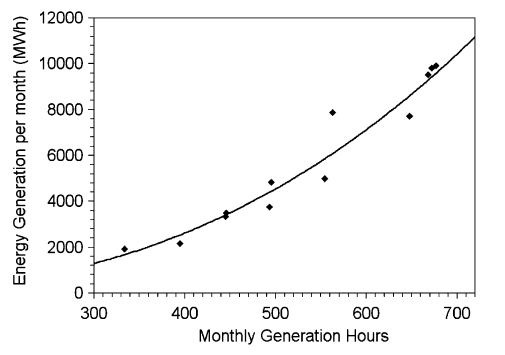
\includegraphics[width=0.8\linewidth,natwidth=898,natheight=587]{billeder/GenerationHourVSGeneration.png}
\caption{The influence of generation hours on energy production \cite{WindPowerGenerationUsingANN}}
\label{fig:energyGenerationFromHours}
\end{figure} 

The Artificial Neural Network trains 3-year dataset containing the mentioned input parameters. The input parameters are during the training compared to the output variable which is the wind energy output of the turbine. See figure~\ref{fig:annArchitecture} for the architecture.
\\[0.5cm]
\begin{figure}[h!]
\centering
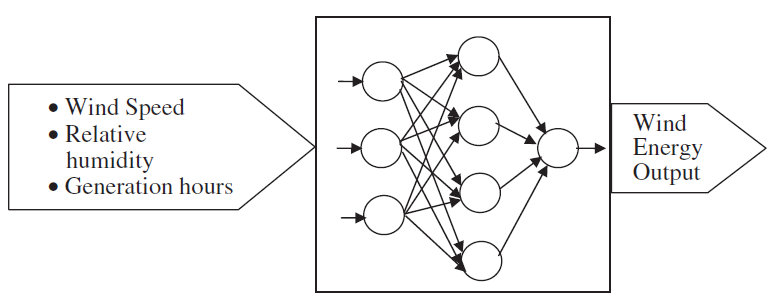
\includegraphics[width=0.7\linewidth,natwidth=898,natheight=587]{billeder/ANNwindSpeedPrediction.png}
\caption{Artificial Neural Network architecture from \cite{WindPowerGenerationUsingANN}}
\label{fig:annArchitecture}
\end{figure}

\subsection{Electricity Prices}
\label{sec:electriciyPrices}
A day-ahead forecasting algorithm that predicts electricity prices in the market based on Neural Network (ANN) and Similar Days Method (SDM) is described in \cite{pjmForecast}. The purpose is to give close estimates for several days to come. The estimates can be used by electricity traders in their decision making but also by transmission companies for different purposes. The companies can use it for scheduling a short-term generator outage in order to predict where it is most inexpensive. It can also be used by actual producers of energy to strategically bid into the market to increase prices. The price estimate itself plays a huge role in decision making in all of these examples.

The combination of ANN and SDM is an attempt to simplify the ANN and make the prediction more accurate. The algorithm forecasts by using a ANN that modifies price curves obtained by averaging five similar price days corresponding to the forecast day, i.e. The ANN corrects the received output from the similar days approach \cite{pjmForecast}. In other words the technique takes into consideration the influence of the most similar days and their price development in relation to the day we wish to forecast.

The ANN is trained with only 45 days from the day before the forecast and 45 days before and after the forecast day in the previous year \cite{pjmForecast}. Results can be seen in table~\ref{table:sdmresult}

\begin{table}[h!]
\centering  % used for centering table
\begin{tabular}{c c c} % centered columns (3 columns)
Year 2006 \#1 & ANN (Avg. MAPE [\%]) \#2 & ANN ( FMSE [\$/MWh] ) \\ [0.5ex] % inserts table 
%heading
\hline                  % inserts single horizontal line
January 20 & 6.93 & 4.57  \\ % inserting body of the table
February 10 & 7.96 & 6.12  \\
March 05 & 7.88 & 5.39  \\
April 07 & 9.02 & 5.87 \\ [1ex] % [1ex] adds vertical space
\hline %inserts single line
\end{tabular}
\caption{Results of forecasting from \cite{pjmForecast}.} % title of Table
\label{table:sdmresult} % is used to refer this table in the text
\end{table}


An explanation for the choice of days is not discussed in the paper. As  mentioned in \cite{18} the more data the more complex problems can be handled

Artificial Neural Networks (ANN) has also been used for electricity price forecasting. In \cite{singhal2011electricity} they use an ANN to predict the half-hourly price of electricity of 24 hours. They differentiate between three different kinds of days: Normal trend price, Price with small spikes and price with large spike. They present a prediction for each of these days and present us to the mean absolute error and the root mean square error, which are standard measures for how accurately the prediction is done. The neural network is fed with 13 inputs as follows \cite{singhal2011electricity}:
\begin{itemize}[noitemsep,topsep=3pt,parsep=2pt,partopsep=3pt]
\item Day of week
\item Time slot of Day
\item Forecasted Demand
\item Change in demand
\item Price (one day ago) - 3 inputs 
\item Price (one week ago) - 3 inputs
\item Price (two weeks ago) - 1 input 
\item Price (three weeks ago) - 1 input 
\item Price (four weeks ago) - 1 input
\end{itemize}
These inputs are fed into a 4-layer neural network: one input layer, two hidden layers and an output layer. The analysis of their ANNs shows that neural networks make a very precise prediction on normal trend price days but have difficulties forecasting the price with small and large spikes. They argue that if the reasons to the spikes in the price were taken into account as inputs in the network maybe the network would be better at forecasting the spikes prices. Also they argue that fuzzy logic, neural networks and dynamic clustering together will provide more efficient forecasting of the prices.
\\[0.5cm]
Since price forecasts in electricity markets are such a volatile operation because of the shifting tides, price demand, holidays etc. that affects the price it can be a cumbersome problem to model. In \cite{amjady2006day} he proposes a new method based on neural networks and fuzzy logics to predict the electricity prices. He calls the new network approach a new fuzzy neural network. Fuzzy logic is basically a logic that has many values or many correct answers. Opposed to binary logic sets, where the answer can be only true or false, in fuzzy logic we have several grades of what we define as true, thus making it harder to decide what is really the truth but also makes us available to have a way larger scale of the data we are looking at.

The fuzzy logic is used within the nodes in the hidden layer to do evaluation of the data inputs. That is the activation function of the neurons in the hidden layer contains a fuzzification function that creates a square of the inputs compared to sinus activation functions that normally takes the sums of the inputs. This square over the inputs is used to classify the inputs into hyper cubes (input spaces) and then calculating how close they are together. Calculation of how far the inputs are from each other are used to calculate the output of the functions. By this we will get an upper and lower limit that the inputs can range between and thus we get a input that has the characteristics which turns out to give a better result than ARIMA, wavelet-ARIMA, MultiLayered ANNs and Radial Basis based ANNs. The data however is not optimized in this paper and they claim this to be future work. They also state that the better performance is based on a limited dataset.

\subsubsection{ARIMA Prediction}
 The Auto Regressive Integrated Moving Average (ARIMA) model is a time series model where the ARIMA processes analyse time series with a class of stochastic processes \cite{EnergyPriceForecasting,ARIMA}. The model has been applied to forecast of commodity prices such as oil, gas and electricity \cite{ARIMA}. 

The success of the presented ARIMA model is dependent on the linear relationship of the underlying data generating process, whereas the Neural Network can handle non-linear relationships \cite{1}. The Neural Networks are simple but a very powerful tool when it comes to forecasting, provided that the training set contains enough data and that enough computational resources are available. 
In \cite{1} the Neural Network outperforms the ARIMA model in terms of both time consumption and accuracy of the predicted price as shown in ~\ref{fig:ArimaVSNN}. where the error percentage to the actual price is shown.
\begin{figure}[h!]
\centering
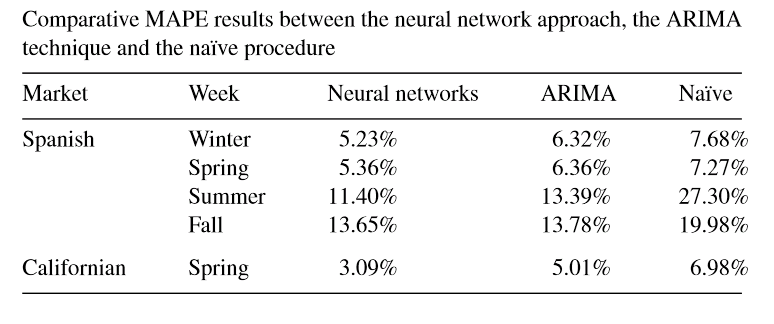
\includegraphics[width=0.8\linewidth,natwidth=898,natheight=587]{billeder/ARIMAvsNN.png}
\caption{Comparison between Neural Network and ARIMA in terms of error \cite{1}}
\label{fig:ArimaVSNN}
\end{figure}
\subsubsection{Support Vector Machine Prediction}
Support vector machines (SVM) can be used for forecasting in the commodity market. In \cite{xie2006new} they use SVMs for predicting the crude oil prices. SVMs are by nature a linear learning machine which means SVMs always use linear functions to solve the regression analysis. However they can be expanded to be able to solve nonlinear problems. This is done by mapping the data into a high-dimensional feature space using a nonlinear mapping. Afterwards it is possible to use linear regression on this space to solve nonlinear problems. The SVMs undergo four different phases before being able to make predictions. These can be seen in figure ~\ref{fig:phasesOfSVM}
\begin{figure}[weight!]
\centering
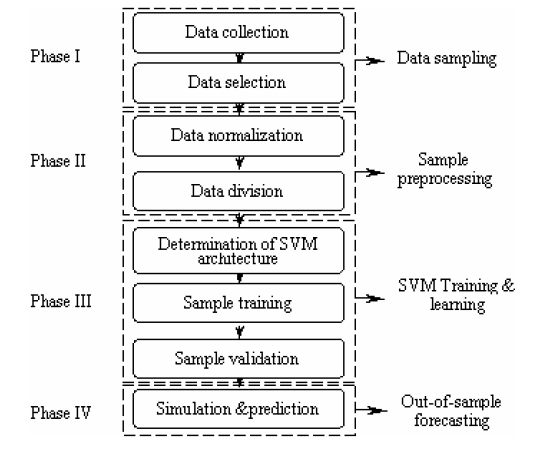
\includegraphics[width=0.8\textwidth ,natwidth=410,natheight=237]{billeder/phases_of_SVM.png}
\caption{The steps taken to create a Support Vector Machine}
\label{fig:phasesOfSVM}
\end{figure}
Data sampling is done daily but due to inconsistencies in these data they adopt weekly and monthly data as alternatives. Data preprocessing is done by transforming the data into more appropriate data for learning purposes. This can be done by using logarithmic transformation or other data transformations. The training and learning step is used for determining the architecture and the parameters of the SVM. There is no criterion for deciding these other than just trial-and-error and the developers experience in the field. Out-of-sample forecasting is done on new data and the prediction is made. As for evaluation they use the Root Mean Square Error (RMSE) to describe the estimated deviation from the real values. Their results and analysis shows that their SVM performs better than both ARIMA and Back Propagation Neural Networks. They argue that SVMs gives better predictions than ARIMA and BPNNs in most cases but neural networks might perform better with data that is optimized for neural networks. Also the neural network outperforms the SVM in one of their sub-period comparisons.

SVMs have also been used for load forecasting of electricity demand. In \cite{chen2004load} they use SVMs to make short-term predictions such as one-day ahead predictions. The goal of this study was to win a competition held by the EUNITE (EUropean Network on Intelligent TEchnologies for Smart Adaptive Systems). This was the winning proposal in the competition. They first examined the data which was half-hourly load demands which had been recorded from 1997 to 1998. In the pursuit of winning the competition they analyzed the data and figured out that in the wintertime load demand was higher than in the summertime thus indicating a connection to weather data and a separation of data was possible. The weekends could also be separated from the weekdays since the weekend load was lower than regular weekdays. When analysis was done they started setting up the model. First of all they prepared the data and selected the data needed for the prediction. They selected calendar attributes to map the holidays and which day it was to account for lower demands. Temperature was included in the vectors used for prediction of the electricity load demand and historical data was incorporated as well. The data segmentation in the steps of preparing a SVM allowed them to take only a subset of the data since most of it could be generalized in the data analysis thus making it easier to do computations. They argue that their model for forecasting demand loads were the best possible model used in this competition and to give a more varied view on this they try out other methods; among these Neural Networks. They configured a neural network that first performed work on the same data as their Support Vector Machine and it provided less than satisfactory feedback with an error margin of 6-8\%. If they took the basic values used in the competition without doing any precomputation on it they received a much better result of 3.64\%. From this they conclude that their SVM performed better than Neural Networks in the specific problem and that neural networks performance depends heavily on the data used as input. 
\subsubsection{Summary}
Artificial Neural Network examples have been presented in the related work section. The characteristics of the electricity prices have been refreshed and different predictions methods have been presented. 
In the description of ANN prediction it is worth observing the input parameters of the network and the way it is modelled. The demand input could potentially consist of input parameters that represents the influential factors for the demand such as the meteorological and socio-economic factors.

ANN can be used in combination with other technologies in an attempt to improve performance and accuracy. This should be considered.
Furthermore, two other examples of predicting and how they relate to ANN is described. This further motivates our choice of ANN as prediction method.   

\subsection{Summary}
This section introduced the concepts and approaches of electricity demand, green energy production and electricity prices. What is somewhat noticeable is the similarity between the influential factors --- especially when it comes to price and demand. They are all dependent on weather data. This indicate that we can approach the wind power production and electricity price prediction with the same Artificial Neural Network simply by replacing the training set and the number of inputs.

\newpage

\section{Decision support}
\subsection{Decision Support Systems}
Since the late 1970s decision support has been a developing area both in the scientific research but also as a tool in the private sector. Decision support is important in that it helps the users to gain an advantage in complex domains and it helps them to take the better decision when it comes down to a crucial choice. Decision support has been applied in many forms over the years and as computers evolve and they become more sophisticated the same applies for the decision support systems (DSS).

In \cite{shim2002past} they argue that DSS are an inevitable evolution in decision making companies across the globe. They describe how DSS systems have evolved from being a conceptual framework to sophisticated software providing information for information heavy companies. In the beginning DSS only existed on standalone computers as a ressource to take into consideration when discussing something with your colleagues. It evolved with the introduction of data warehouses and the world wide web into a more analytic tool, called on-line analytic processing, that gathered information from data warehouses and compiled this information into behavioural information about customers or the like. This was decision support based on datamining and analysis of the data. Also the introduction of the internet (as we know it) reduced the costs of bringing DSS to smaller cooperations and firms and made it easier for people to use this software in their everyday work scenario. This also introduced collaborative support systems that are systems focused on helping groups of people rather than just a single individual. These types of decision support systems often spans more than just small groups of users and incorporates entire organisations into one decision support system. While these systems are interesting we wont be covering them here becaues they are out of the scope of this thesis. Instead we will be looking at Optimization-based support models. These DSS can be divided into three stages formulation, solution and analysis\cite{shim2002past}:
\begin{quotation}
\textit{Formulation refers to the generation of a model in the form acceptable to a model solver. The solution stage refers to the algorithmic solution of the model. The analysis stage refers to the 'what-if' analyses and interpretation of a model solution or a set of solutions.}
\end{quotation}
The formulation support is about narrowing down the problem and normalizing the data so that it fits into a datamodel or an algorithm. The solution stage involves faster and better algorithms that will solve complex problems at a higher rate. At the same time people use more sophisticated methods to solve combinatorial problems. This is done by using genetic algorithms, neural networks and the likes\cite{shim2002past}. The last part is analysis where the DCC focuses on delivering the information from stage 2 and handing it over to the client in a useable form instead of just the analysis which the client then have to make sense off. This can be done by presenting the user for spreadsheets, graphs and report generation.

In the future \cite{shim2002past} argue that:
\begin{quotation}
\textit{(i) it should look for areas where the proven skills of DSS builders can be applied in new, emergent or overlooked areas; (ii) it should make an explicit effort to apply analytic models and methods; it should embody a far more prescriptive view of how decisions can be made more effectively; (iii) it should exploit the emerging software tools and
experience base of AI to build semi-expert systems, and (iv) it should re-emphasise the special value of DSS practitioners as being their combination of expertise in understanding decision making and knowing how to take advantage of developments in computer-related fields.}
\end{quotation}
By this they are saying that they predict a future with more sophisticated decision support systems that in a broader manner will use artificial intelligence to provide the support. They also argue that with the ability to distribute products over the internet and easily reach a broader audience more specialised DSS will pop up. They foresee that a lot of these services will be on a pay per use basis where you log into a system and get the information you are after and pay as you use it.

\subsection{Presentation of Uncertain Information}
\label{sec:uncertainInformation}
It is necessary to get a complete understanding of uncertainties in the data you wish to present and an adequate way of visualizing it to the user. This becomes even more important when the information is to be used in dynamic environments where high-risk decisions have to be made \cite{UncertainInformation}. Furthermore, new technologies have made it possible to analyze and compare data from multiple sources which can create an information overload that makes decision-making even more difficult. The Decision Support System (DSS) as described above can combine and present all of this information in order to support users in their attempt to make the best decision. However, autonomous systems does not always guarantee the best result or performance. It can actually contribute to creation or exposing of uncertainties when dealing with complex environments such as financial markets \cite{UncertainInformation} if not handled carefully. It necessary to present the uncertain information in the most appropriate way.
\\[0.5cm]
Most people are met with uncertainties on a daily basis. We are fully aware that decisions have to be made even though information is not exact or complete. Often this results in decisions based on guesses and assumptions \cite{UncertainInformation}. When dealing with high-risk decisions it is necessary to be aware of the uncertainties so that it can be accounted for when taking the actual decision. 
There are different types of uncertainties and it can be characterized as both subjective and objective (see figure~\ref{fig:typesOfUncertainty}). 
\begin{figure}[h!]
\centering
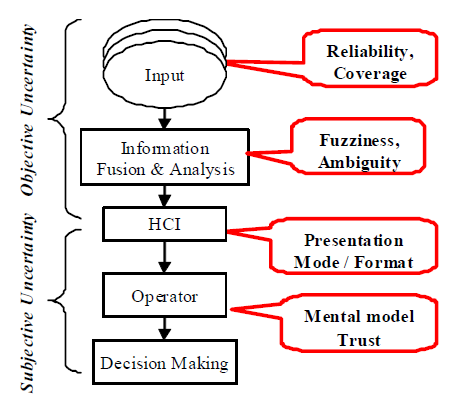
\includegraphics[width=0.7\linewidth,natwidth=898,natheight=587]{billeder/TypesOfUncertainInformation.png}
\caption{Types of uncertainty from \cite{UncertainInformation}}
\label{fig:typesOfUncertainty}
\end{figure}  
The objective uncertainties is the acquisition and processing of the data, and the output. Is the data acquired from a trusted source, is it comprehensive enough and does processing impact the data precision. We are combining and comparing information from different sources during the data processing which can bring uncertainties such as conflicting data or just bad estimates. This information needs to be brought to the users attention so they can act on it. The subjective uncertainties arise in the mind of the user when he is to make a decision. People perceive, interpret and process information differently depending on their background. It is not enough to simply present the information. It is essential to visualize and present the information specifically to the users of the system. Decisions also depend on the specific task, the context, needed accuracy, time constraint, level of risk and experience. 
\\[0.5cm]
Five strategies for user decision making in an uncertain environment is presented in \cite{UncertainInformation}. 
\begin{itemize}
\item Reduction: collecting further information to reduce uncertainty.
\item Assumption-based reasoning: Fill in gaps by relying on experience and imagination, or make sense of factual information.
\item Weighting pros and cons of alternatives
\item Forestalling: Prepare what to do in case of a potential negative result
\item Suppressing uncertainty by simply ignoring it. Last resort.
\end{itemize}  
This emphasizes the need for making the users aware of potential uncertainties in the information e.g. situation awareness. What strategy to use relies greatly on how much uncertainty. The uncertainties should always be made aware to the users so that it is not necessary for them to check the validity themselves. It is furthermore important that the user understands the basic logic of the algorithm so that the answer is not just "black magic". They need to trust it.
\\[0.5cm]
The way of presenting information greatly impacts the decision making process. People can process more data and do it more quickly when it is presented graphically rather than in text \cite{UncertainInformation}. This does not imply that the information can be overloaded with graphical information; it is still important to only show what is most critical for the user to make the best decision. An example of a graphical representation that is perceived quickly is \textit{blurred or degraded graphical images} where the images in a natural way visualizes the amount of uncertainty by blurring it accordingly (see figure ~\ref{fig:blurryIcons}). 
\begin{figure}[h!]
\centering
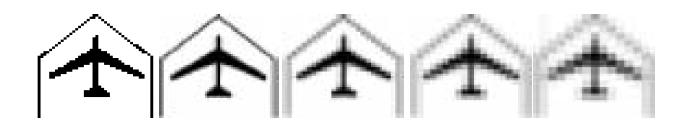
\includegraphics[width=0.7\linewidth,natwidth=898,natheight=587]{billeder/blurryIcons.png}
\caption{Blurry icons from \cite{UncertainInformation}}
\label{fig:blurryIcons}
\end{figure}  
\\[0.5cm]
Based on the discussions in \cite{UncertainInformation} they present a number of high level guidelines for presenting uncertainty. To summarise the most prominent:
\begin{itemize}
\item Always define and present uncertainty and accuracy of data.
\item Present uncertainty at all time and not only when the decision has to be made.
\item Identify the user so that the system can be aligned with their way of reasoning and thinking. This include basic understanding of the underlying algorithm.
\item Provide conflict in data if it is present.
\item Graphical distortion can be improve performance when showing uncertainties.
\item Graphical presentation is not as precise a numerical but they can support each other in achieving precision and performance.
\item Users must be able to restructure the information environment themselves so that it fits their need and way of thinking.
\end{itemize}
The guidelines can be used when developing interface prototypes for Decision Support Systems (DSS).
\subsection{Summary}
KRIST SKRIVER OM DSS.

Decision Support System interfaces must integrate and show uncertain information. The users must be made aware of any information that can have an affect on their decision. Guidelines for visualizing and structuring of information to support the best decision making is presented. These can be used as a starting point for our DSS.

%%%%%%%%%%%%%%%%%%%%%%%%%%%%%%%%%%%%%%%%%%%%%%%%%%%%%%%%%%%%%%%%%%%%%%%

\chapter{Dataset Analysis}
This chapter will analyze what influence the price and wind production. The analysis will contribute to locating the potential input parameters to be used in the Artificial Neural Network. 
\label{ch:theANNs}
\section{Data Collection}
\label{sec:dataCollection}
Section~\ref{sec:predictionSection} describes the concepts of prediction within the area of wind production and electricity prices. What is important to emphasize here is the type of input data used for the prediction of both price and production. Meteorological factors are important in both cases and can therefore be extracted from the same source. The second type of data is the prices and the productions themselves. Artificial Neural Networks calculates a generalized function by looking at historical data and comparing with the actual values (Section~\ref{sec:annSection}), e.g. comparing the weather factors at time t with the actual production at time t. For this reason it is necessary to collect historical meteorological, price and production data in order to do the prediction. A simple drawing of the input and outout can be seen in Figure~\ref{fig:verySimpleANN}.

\begin{figure}[H]
\centering
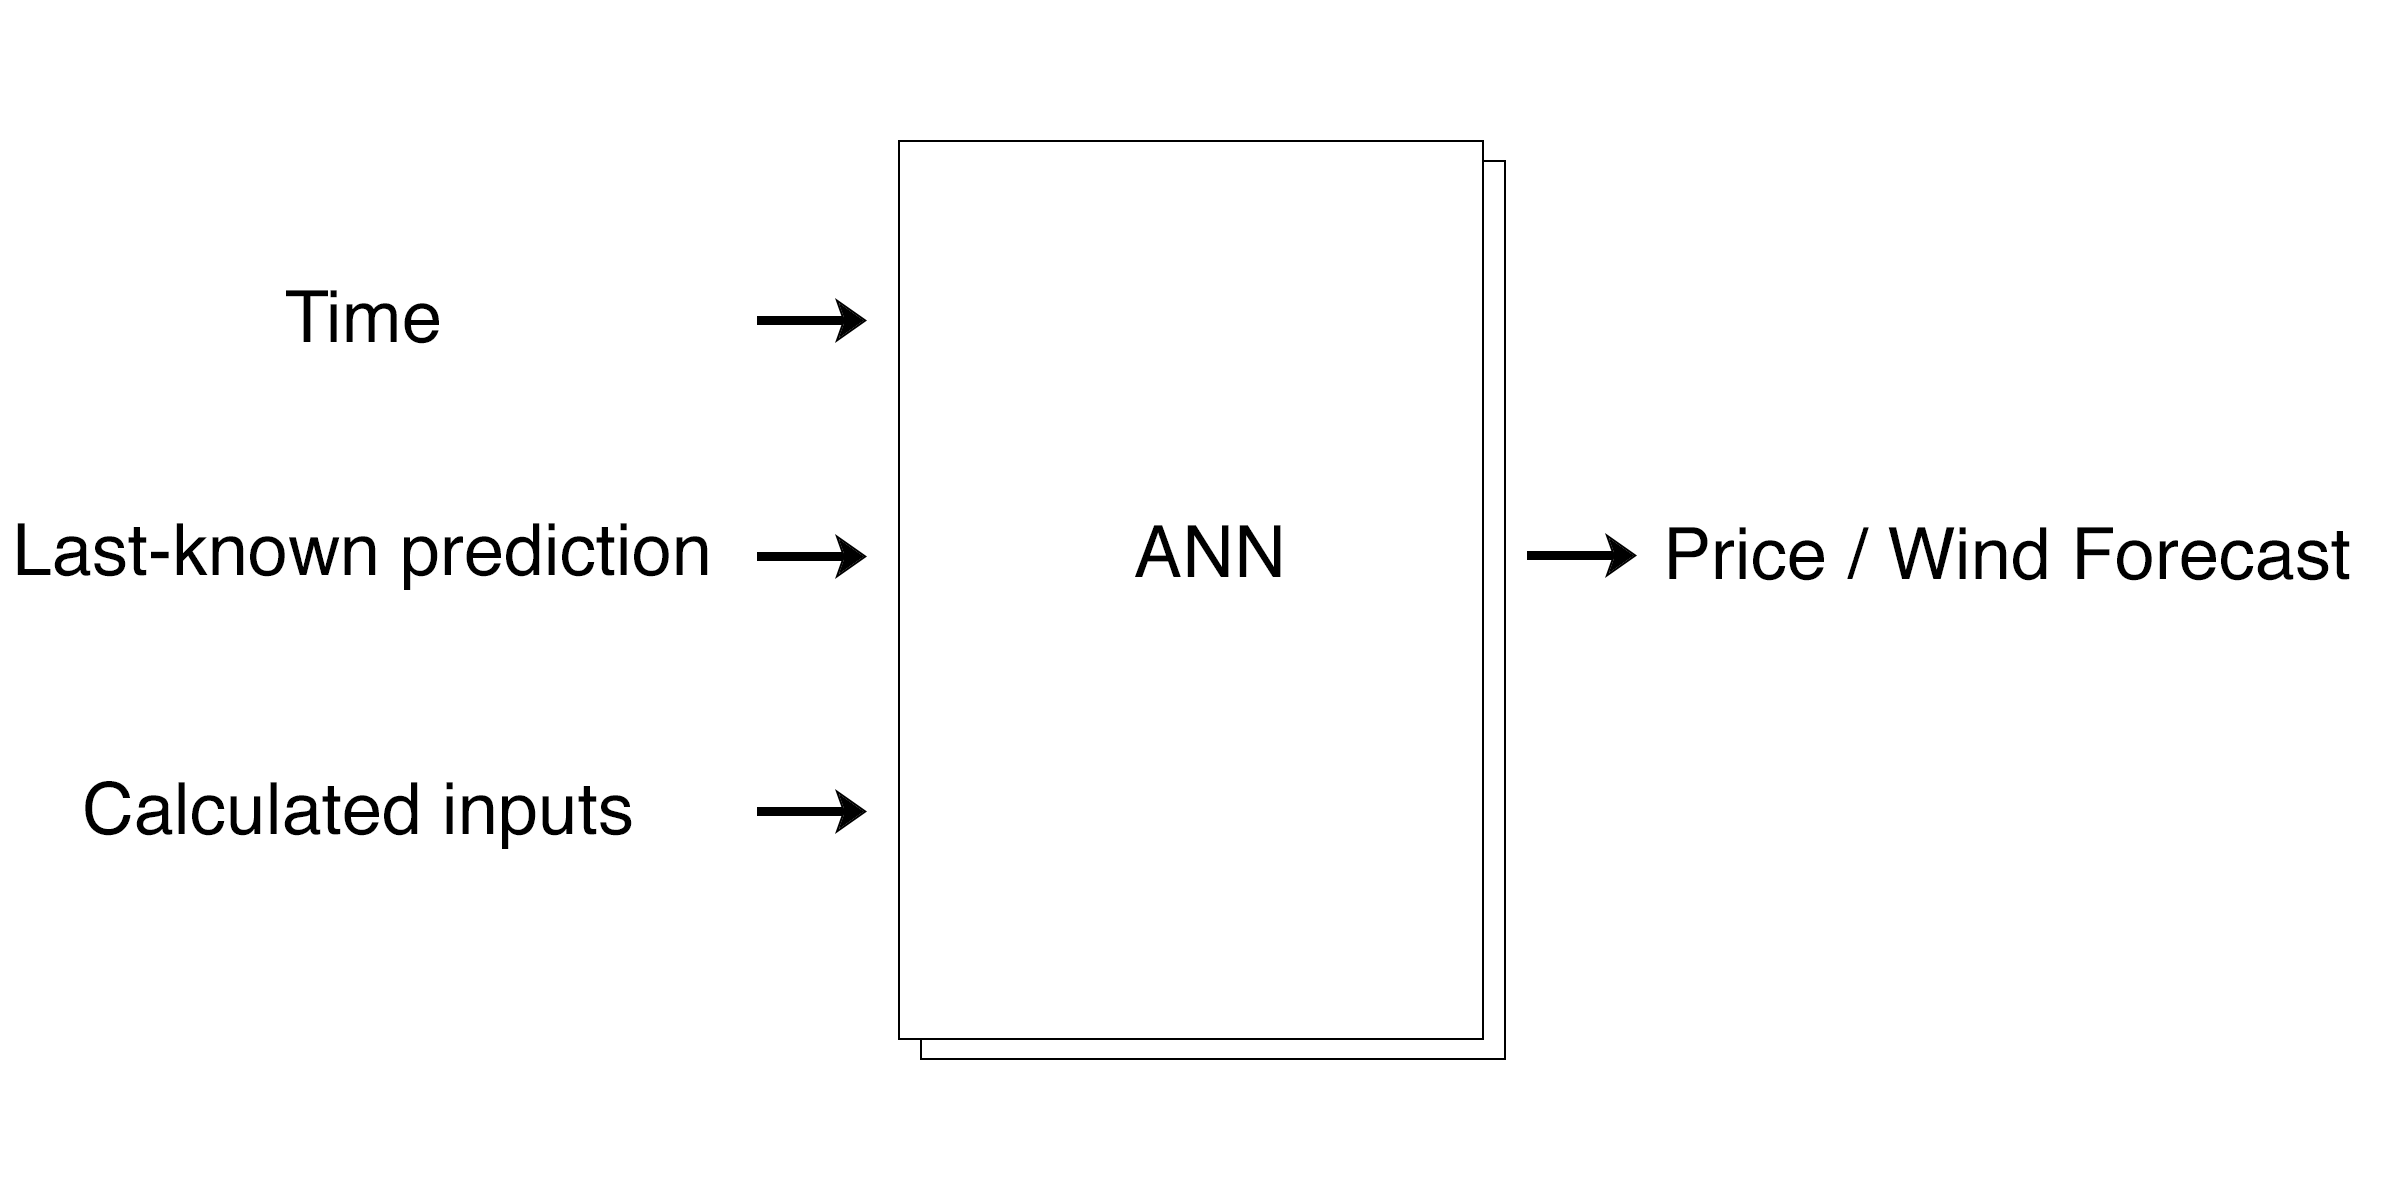
\includegraphics[width=0.85\linewidth,natwidth=898,natheight=587]{billeder/simpleANN.png}
\caption{Simple ANN -- VERY UGLY DRAWING NEED REPLACE}
\label{fig:verySimpleANN}
\end{figure}

The data must come from a trusted source so that proper predictions can be based on it. The data must be of a certain quality in relation number of observations because we need to make hourly predictions, e.g. the meteorological observations must be within an interval of 60 minutes or else we ill ignore data from that particular station.

The National Oceanic and Atmospheric Administration's (NOAA) National Climatic Data Center (NCDC) provides public access to all climate and historical weather data from various weather stations around the world\footnote{\url{http://www.ncdc.noaa.gov/}}. We have used it for collection of historical weather data from various Danish weather stations that delivers observations from at least every hour. The data is in a fixed length format and contains all the necessary weather data for prediction. Format can be seen in \todo{BILAG 11111}. 
The historical hourly price and wind production data has been downloaded from nordpoolspot\footnote{\url{www.nordpoolspot.com}} in excel format BILAG2.
The data will be aggregated into one file that contains the needed input and output parameters for both prediction of price and wind production. The file includes all meteorological factors, prices, consumptions and wind productions from every hour of the last two years. 

For the sake of simplicity we will be focusing on West Denmark and Funen which is also known as DK1 in the electricity market [find ref]. The collected data will be validated through plot diagrams that show and establish the relationships between weather conditions and the power generation/price of DK1.

The weather data is collected from all available weather stations in DK1 from NOAA~\ref{fig:stations4average} - some stations have been omitted due to missing data. The collected data will be averaged and used as basis for creating training sets to be used as input parameters for the Artificial Neural Networks. It is necessary to average the weather data to get a representative picture for all regions included in DK1 because only one price and production exist for all of DK1.

\begin{figure}[H]
\centering
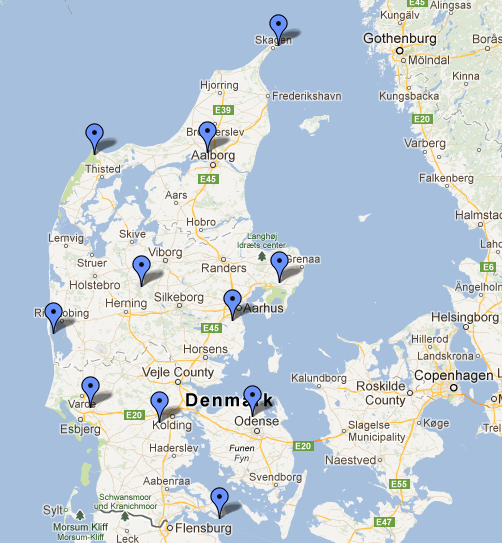
\includegraphics[width=0.85\linewidth,natwidth=898,natheight=587]{billeder/stations4average.png}
\caption{Selected weather stations in DK1}
\label{fig:stations4average}
\end{figure}


We will remove data that is obscure and is related to conditions we cannot predict. (See trimming~\ref{sec:Trimming})
\section{Wind Power Analysis}
\label{sec:windPowerAnalysis}
The purpose is to predict the total hourly wind production available on the energy market from all of western Denmark (DK1) with enough accuracy to make a green decision. It is important to note that it is the wind production available on the market and not the entire production of Western Denmark. The entire wind production would be much higher and is not all distributed through the deregulated market\ref{FIND ONE} - fx. vindstoed and private owned. This can also be seen by the correlation between consumption and wind production in Table~\ref{table:pearsonCoeficientWindProduction} and Figure~\ref{fig:consumptionVsWindProduction} which indicates that the production is moved into the market when the demand for electricity is high. Because the wind production follows market trends it is necessary to consider economical and statistical factors of the current market situation when predicting the production. It is our intention to get a close enough estimate so that it can be used as an indicator for the hourly amount of wind production in the market for the next 24 hours.
Most others have been forecasting the wind production for specific wind farms where exact weather conditions and wind mill throughput of the site was known. The assumption is that we loose accuracy without the actual throughputs of the windmills because it is directly proportional to the meteorological factors as presented in~\ref{sec:windmillPlacement}. 

This is also more critical in the other examples because it is used to place the mills or the predict how much electricity the mill can sell the next year - a large investment would be lost if placed wrong. 

It is not surprising that weather conditions directly impact the wind power generation. The typical input parameters for wind power prediction are wind speed, air density, temperature and pressure \cite{WindPowerGenerationUsingANN} with the most influential factor being wind speed because it is directly converted to power in the wind turbine. The following subsections will describe the parameters relationship to wind production and how it is used in the modelled ANN.

The Pearson Correlation Coefficient\footnote{\url{http://en.wikipedia.org/wiki/Pearson_product-moment_correlation_coefficient}} has been used to establish the linear dependency between meteorological factors, consumption and wind production. Table ~\ref{table:pearsonCoeficientWindProduction} shows this correlation coefficient. The factors have been discussed throughout the thesis as having an influence on the wind speed production to some degree. The Pearson Correlation Coefficient returns a value between -1 and +1 which indicates the strength of the linear correlation between two variables.

\begin{table}[H]
\centering  % used for centering table
\begin{tabular}{c c} % centered columns (3 columns)
Input factor & Pearson Correlation Coefficient \\ [0.5ex] % inserts table 
%heading
\hline                  % inserts single horizontal line
Consumption & 0.61 \\ % inserting body of the table
Wind Speed & 0.94 \\
Temperature & -0.09 \\
Wind Direction & 0.21 \\ [1ex] % [1ex] adds vertical space
\hline %inserts single line
\end{tabular}
\caption{Table showing Pearson correlation coefficient between various factors and the wind production.} % title of Table
\label{table:pearsonCoeficientWindProduction} % is used to refer this table in the text
\end{table}

It is obvious from Table~\ref{table:pearsonCoeficientWindProduction} that consumption and wind speed are the most direct influential factors. The consumption or demand can become a problem because it also needs to be predicted and if this prediction shows to be inaccurate then it will add the error to the wind production forecast.  (ADD MORE LIKE DENSITY, DEW POINT, HUMIDITY, TIME OF DAY, ECT).

\subsection{Meteorological factors}

\subsubsection{Wind Speed}
The relationship between hourly wind speed and hourly wind power production of DK1 is seen in Figure~\ref{fig:windVsProd}. The graph clearly shows the expected impact of wind speed on the wind energy production.

\begin{figure}[H]
\centering
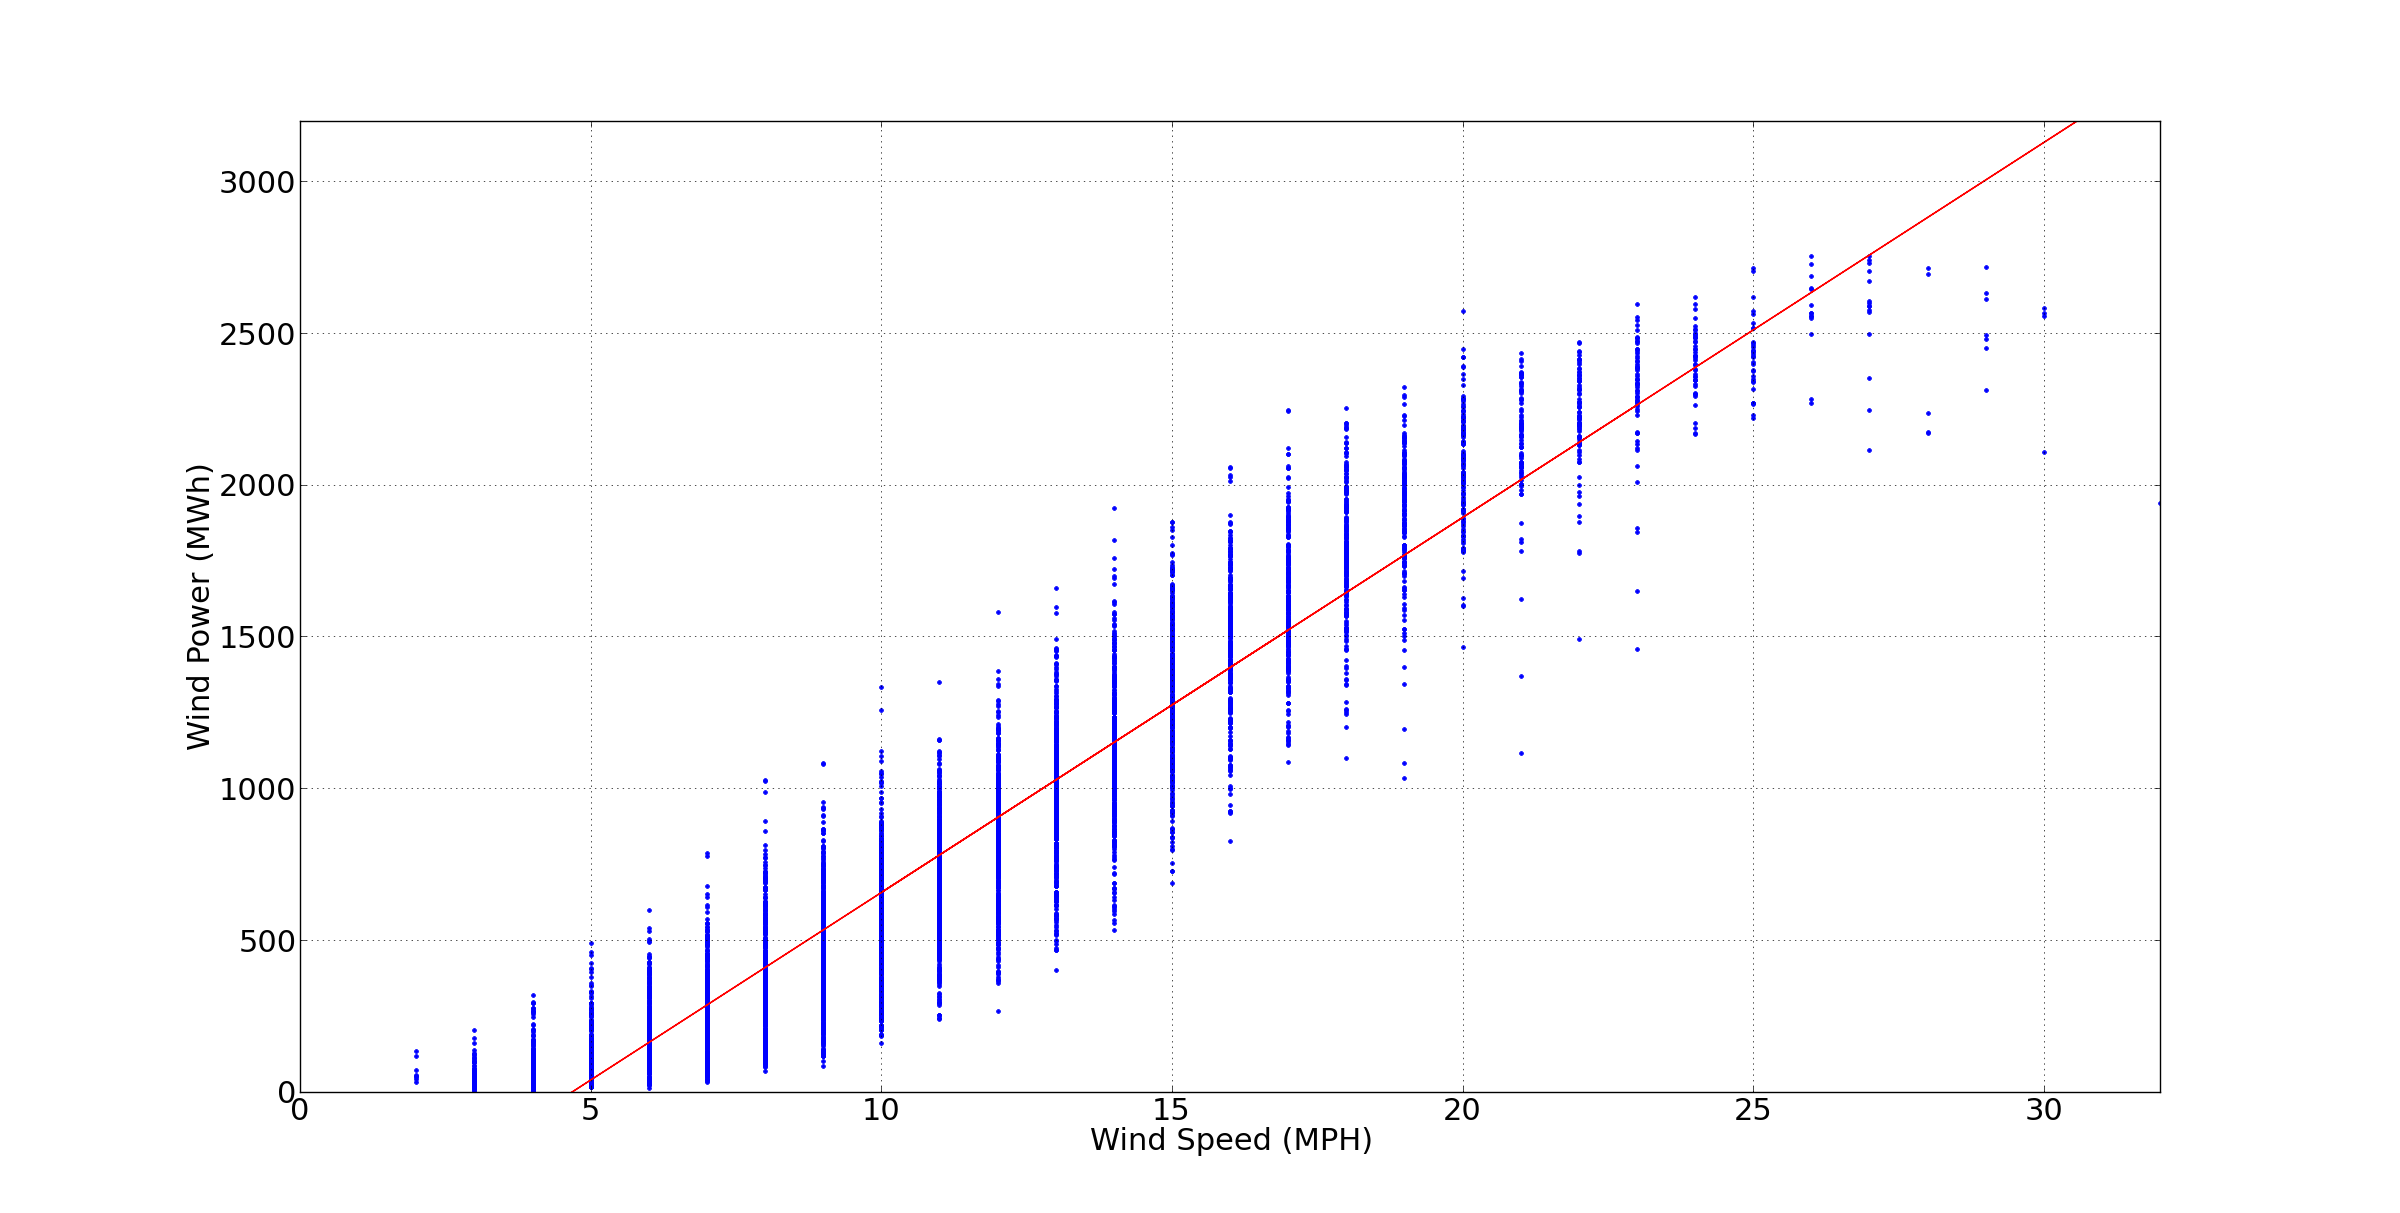
\includegraphics[width=0.99\linewidth,natwidth=898,natheight=587]{billeder/WindSpeedVsProduction.png}
\caption{Wind speed vs. wind production in 2012}
\label{fig:windVsProd}
\end{figure}

What is noticeable from the graph is wide range of productions that is covered by a relatively small number of wind speeds. Wind speed 15 can cover wind productions all the way from 700 to 1900 and therefore other input parameters are needed to point us in the right direction within these interval. 

\subsubsection{Air Density}
\label{sec:airDensity}
It is described in~\ref{sec:windmillPlacement} that wind energy is proportional to air density where a higher density means more power for a specific wind speed. This does not imply that a higher air density is equal to higher wind power production in general because it depends on the wind speed. Days with equal wind speed but variation in air density should show an increase in power production when the air density is highest. 

Air density depends directly on temperature and pressure which can be described by $Air Density=\frac{P*M}{(R*T)}$ where R is a gas constant and M is the density of air. The monthly pressure in Denmark has low variation compared to the temperature as shown in Figure~\ref{fig:pressureTemperatureVariance}. For this reason, the temperature will have the most influence on the air density in Denmark. The formula express that when temperature decreases the air density will increase linearly, e.g. the wind power production for a specific wind speed will be higher in times of low temperature. The air density has been calculated for every hour in the training set and the correlation has been established for each wind speed in Table~\ref{table:pearsonCoeficientAirDensity}. The wind power production increases with the air density for each wind speed as described by the formula.

\begin{figure}[H]
\centering
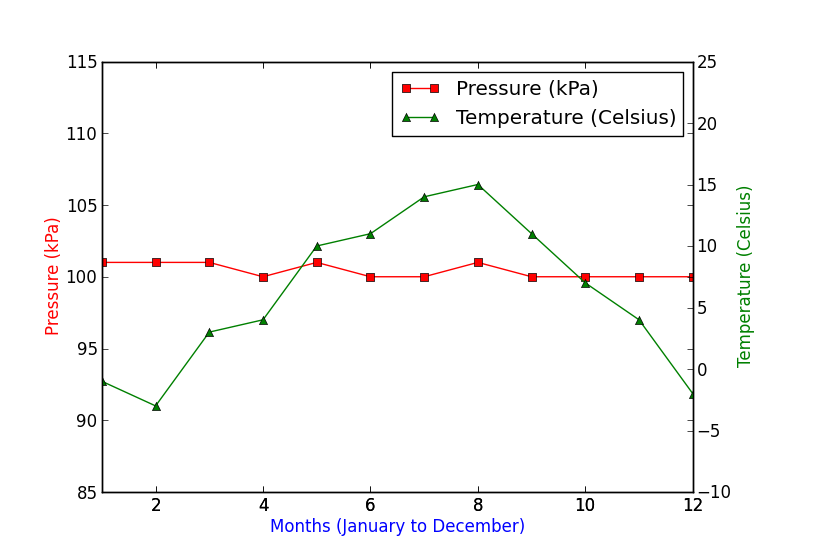
\includegraphics[width=0.99\linewidth,natwidth=898,natheight=587]{billeder/pressureTemperatureVariance.png}
\caption{Temperature and Pressure variance for 2012}
\label{fig:pressureTemperatureVariance}
\end{figure}

\begin{table}[H]
\centering  % used for centering table
\begin{tabular}{c c} % centered columns (3 columns)
Wind Speed (mph) & Pearson Correlation Coefficient for Air Density \\ [0.5ex] % inserts table 
%heading
\hline                  % inserts single horizontal line
2 & 0,29\\ \hline
3 & 0,38 \\ \hline
4 & 0,28 \\ \hline
5 & 0,18 \\ \hline
6 & 0,27 \\ \hline
7 & 0,26 \\ \hline
8 & 0,29 \\ \hline
9 & 0,31 \\ \hline
10 & 0,28  \\ \hline
11 & 0,18 \\ \hline
12 & 0,19 \\ \hline
13 & 0,19 \\ \hline
14 & 0,19 \\ \hline
15 & 0,12 \\ \hline
16 & 0,10 \\ \hline
17 & 0,22 \\ \hline
18 & 0,11 \\ \hline
19 & 0,28 \\ \hline
20 & 0,11 \\ \hline
21 & 0,18 \\ \hline
22 & 0,18 \\ \hline
23 & 0,26 \\ \hline
24 & 0,01 \\ \hline
25 & 0,12 \\ \hline
26 & 0,20 \\ \hline
27 & 0,72 \\ \hline
28 & 0,87 \\ \hline
29 & 0,61 \\ \hline
30 & 0,76 \\ \hline  
Average: & 0,28 \\ [1ex] % [1ex] adds vertical space      
\hline %inserts single line
\end{tabular}
\caption{Table showing Pearson correlation coefficient between the various wind speeds in the dataset and the air density.} % title of Table
\label{table:pearsonCoeficientAirDensity} % is used to refer this table in the text
\end{table}

\subsubsection{Wind Direction}
Figure~\ref{fig:windDirVsProd} shows that the wind direction in general has an impact on the wind production. Wind mills are turning in the direction of the wind which could make these numbers a coincidence. The answer could be that the wind speed is more powerful when coming from the west. This relationship is established in Figure~\ref{fig:windDirectionVersusWindSpeed}. It needs to be validated in experiments if the wind direction makes sense in relation to the other parameters used as input. \todo{show compass and show the relation between west wind and more powerful speeds
 }.   
 
\begin{table}[H]
\centering  % used for centering table
\begin{tabular}{c c} % centered columns (3 columns)
Input factor & Pearson Correlation Coefficient \\ [0.5ex] % inserts table 
%heading
\hline                  % inserts single horizontal line
Wind Production & 0.21 \\ % inserting body of the table
Wind Speed & 0.20 \\ [1ex] % [1ex] adds vertical space
\hline %inserts single line
\end{tabular}
\caption{Table showing Pearson correlation coefficient between various factors and the wind direction.} % title of Table
\label{table:pearsonCoeficientWindDirection} % is used to refer this table in the text
\end{table}

\begin{figure}[H]
\centering
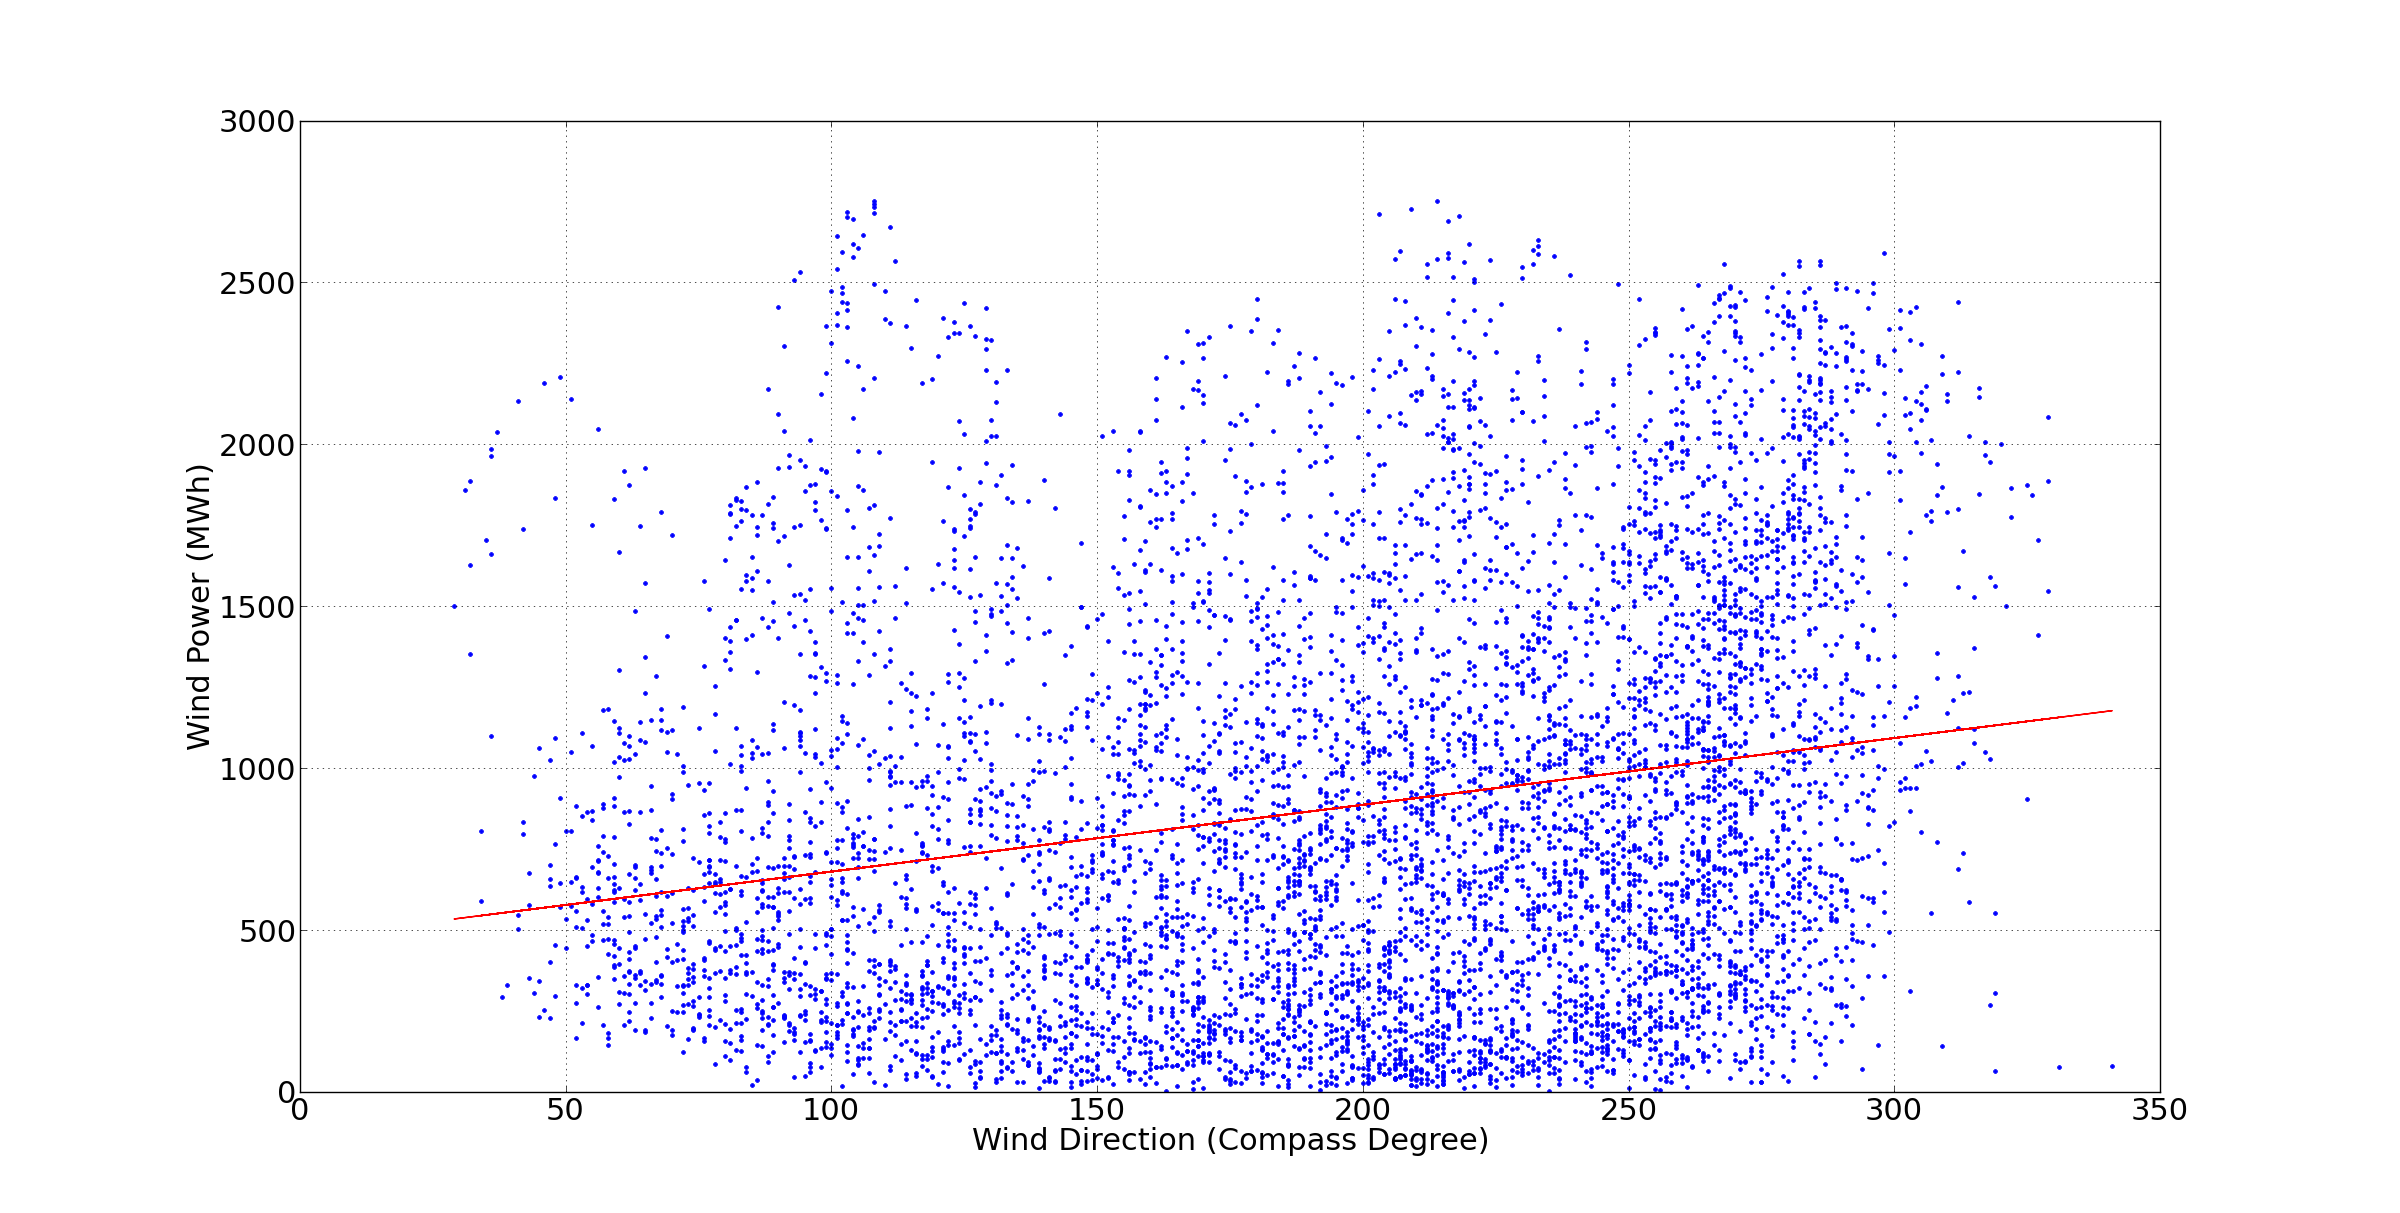
\includegraphics[width=0.99\linewidth,natwidth=898,natheight=587]{billeder/productionVsWindDirection.png}
\caption{Wind Direction vs. wind production in 2012}
\label{fig:windDirVsProd}
\end{figure}

\begin{figure}[H]
\centering
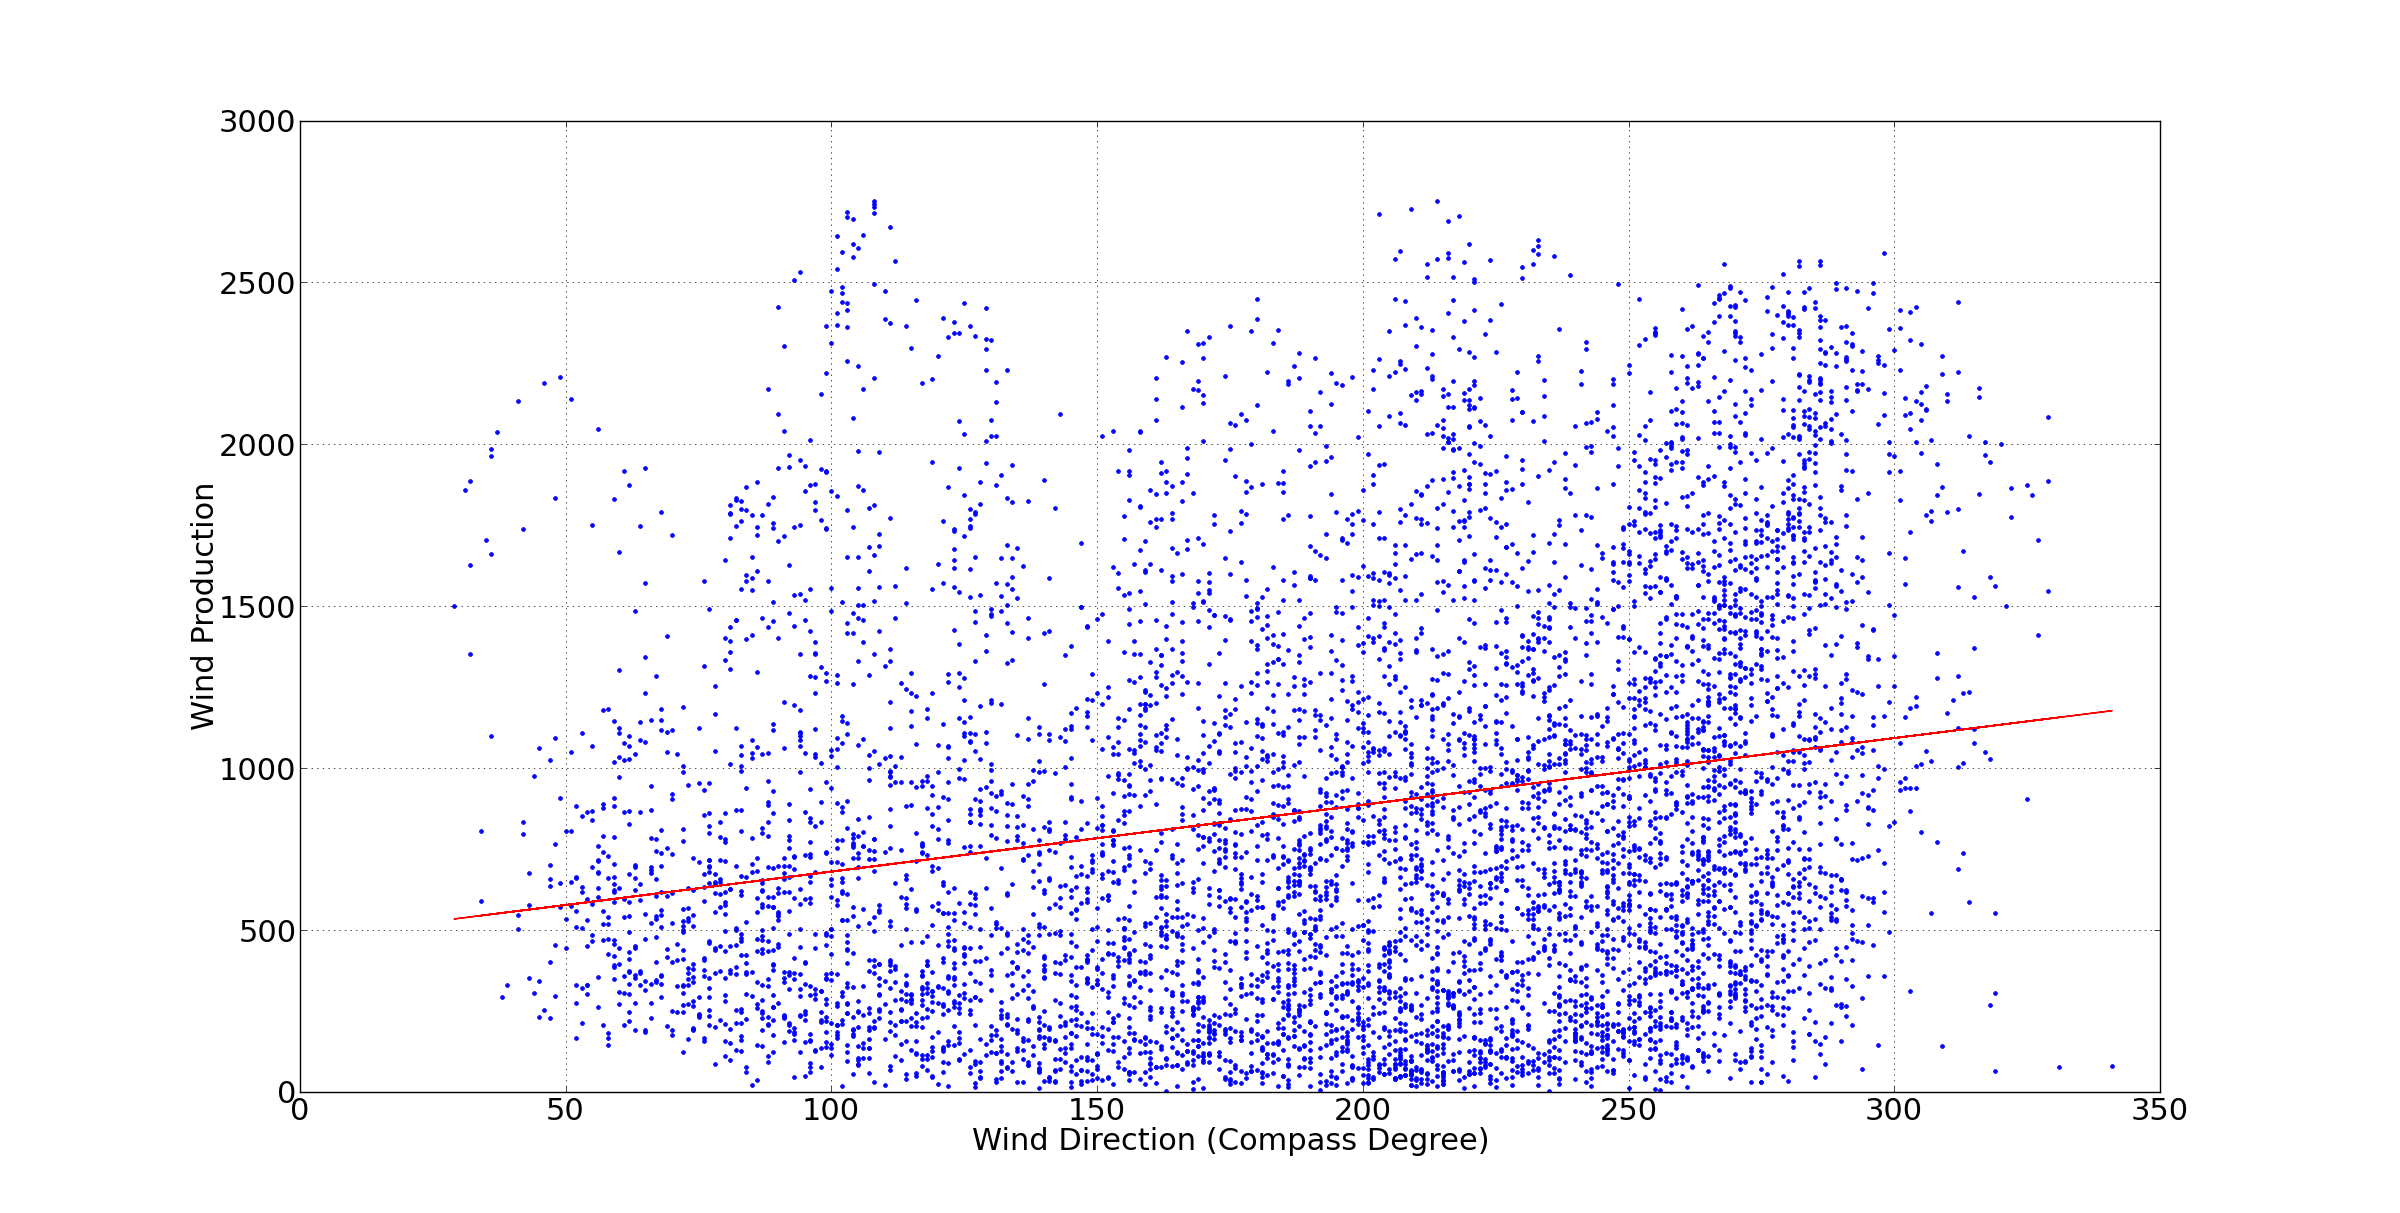
\includegraphics[width=0.99\linewidth,natwidth=898,natheight=587]{billeder/windDirectionVersusWindSpeed.png}
\caption{Wind Direction vs. wind production in 2012}
\label{fig:windDirectionVersusWindSpeed}
\end{figure}

\subsection{Other factors}

\subsubsection{Consumption}
It is expected that the wind power available on the energy market will be low at times with low consumption, e.g if no energy is needed the wind power can't be sold.  This relationship is shown in Figure~\ref{fig:consumptionVsWindProduction}. This also tells us that the wind production is connected to the market and cannot be deduced only from meteorological factors.

\begin{figure}[H]
\centering
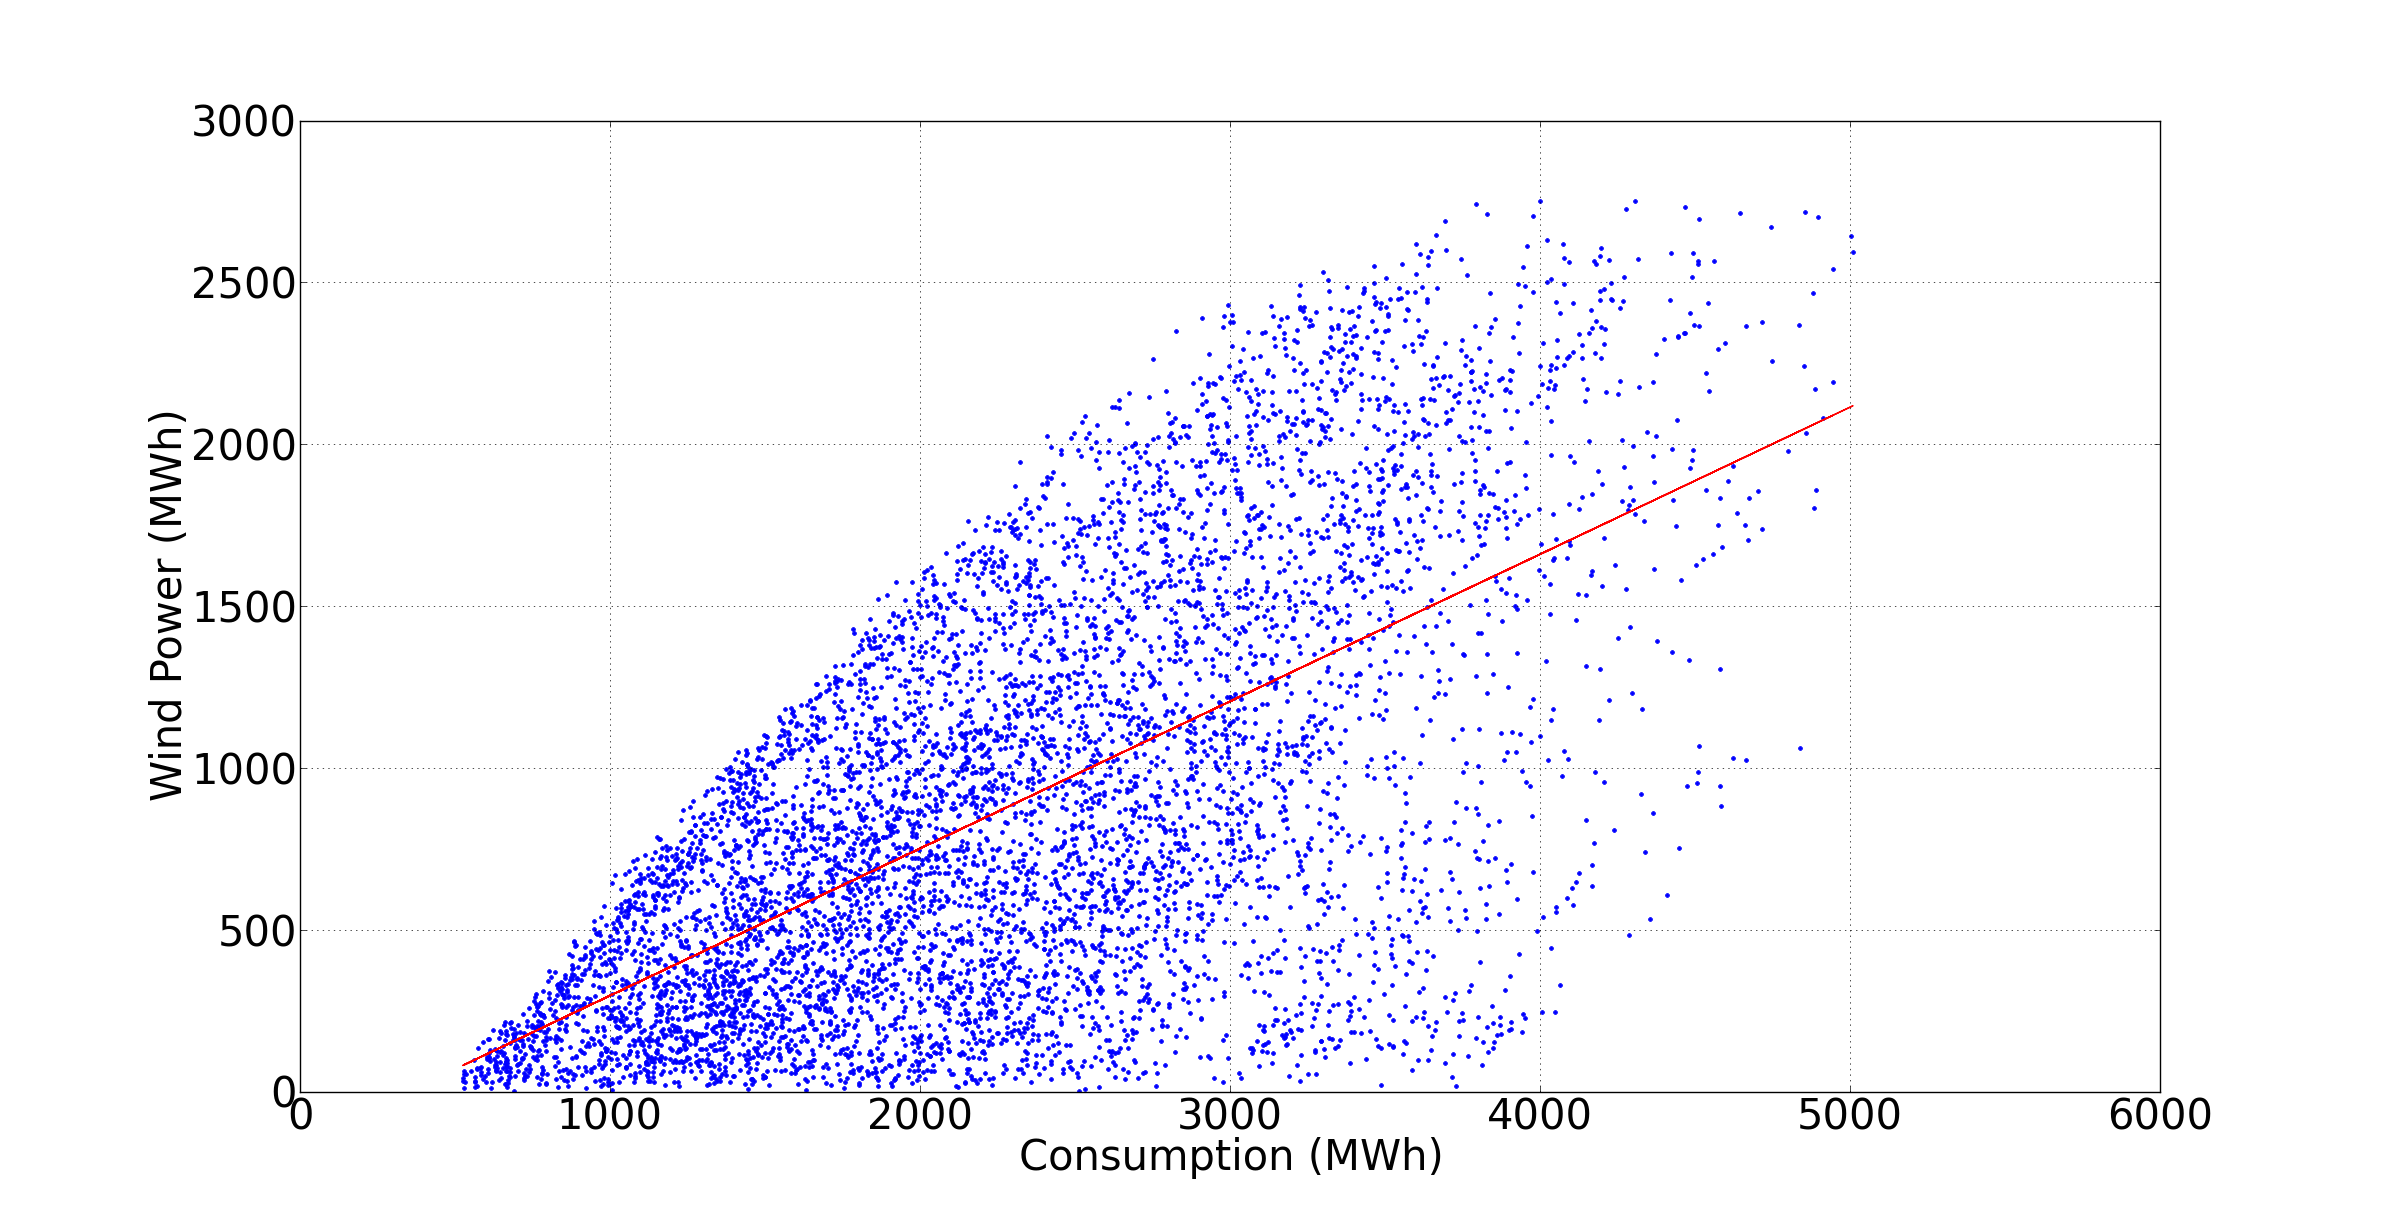
\includegraphics[width=0.99\linewidth,natwidth=898,natheight=587]{billeder/consumptionVsWindProduction.png}
\caption{Consumption vs. Wind Production in 2012}
\label{fig:consumptionVsWindProduction}
\end{figure}

It can be a disadvantage to use consumption as input since we will rely on predictions from nordpool spot - it is out of scope for this thesis to predict it in its own Neural Network. Following section~\ref{sec:ElectricityDemand} the demand is much controlled my the meteorological factors which can make it sufficient to include these as a substitute for the actual demand. The temperature impact on demand can be seen in Figure~\ref{fig:consump_temp_green}. We will compare the two approaches in experiments to come.

\begin{figure}[H]
\centering
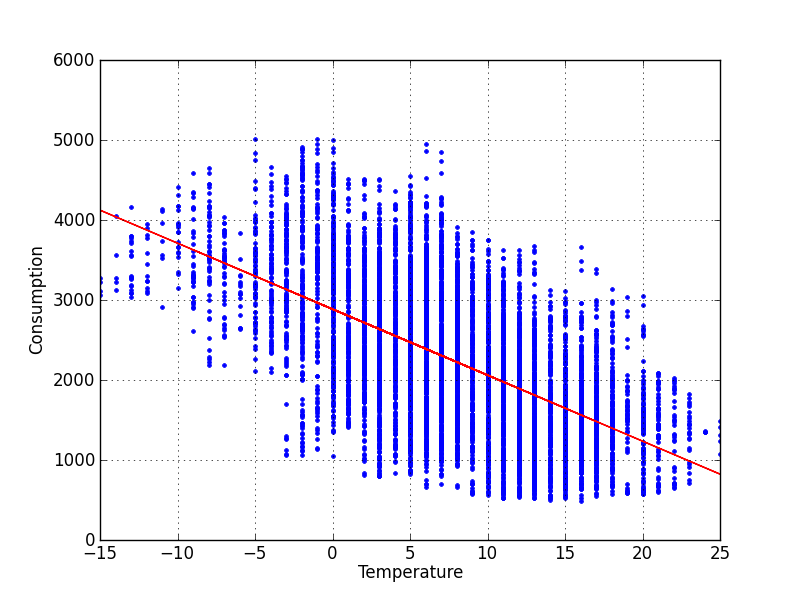
\includegraphics[width=0.8\textwidth ,natwidth=410,natheight=237]{billeder/energy_price_plots/consump_temp.png}
\caption{Demand and temperature plot.}
\label{fig:consump_temp_green}
\end{figure}

\subsubsection{Time of day}
The dataset consists of all hours of the years included. Based on this the network is going to forecast multiple hours ahead and it therefore necessary to establish if any correlation between the time of day and the wind production exist. The average wind production distribution for a calendar day can be seen in Figure~\ref{fig:hourly_wind_production}. The wind production is at its highest during the day from 8-20 and therefore it is needed to use the time of day as input parameters.  

\begin{figure}[H]
\centering
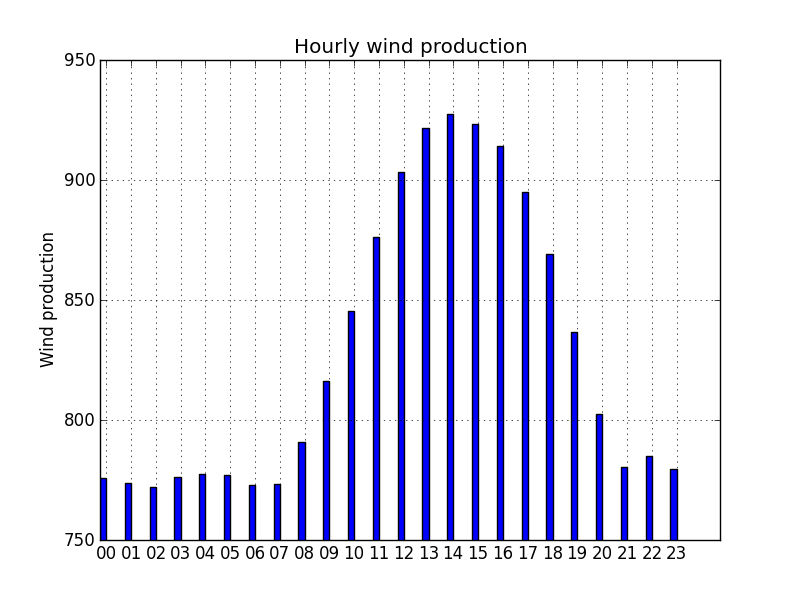
\includegraphics[width=0.99\linewidth,natwidth=898,natheight=587]{billeder/hourly_wind_production.png}
\caption{Time of day vs. Wind Production in 2012}
\label{fig:hourly_wind_production}
\end{figure}

\subsection{Wind Production Development}
\label{sec:windProductionDev}
The above analysis shows the wind production development to be much dependent on wind speed and air density together with the general trend on the market. 

The high volatility in the wind production is very clear when considering the development curve in Figure~\ref{fig:windHourDevelopment400Hours}. This is not a problem if the correlation between the input parameters result in a low number of output possibilities because the generalization of the ANN then would be enough. This is not the case for our input parameters for wind productions and an example of such can be seen in Figure ~\ref{fig:inputParameterDistribution} where outputs for similar inputs are shown --- the input limits can be seen in Table~\ref{table:similarHoursLimitsWindProd}. The generalization would lean towards 898-1048 but if the last wind production was 1198 and the tendency rising then the prediction would be better off guessing above or around 1198. This can be further supported by Figure~\ref{fig:windHourDevelopment400Hours} which illustrates the tendency of the production curve and the need to consider the immediate past because of its significance for the movements to come. It is necessary to identify these tendencies in every hour in order to predict the wind production more accurately. The concept of tendency as input is discussed in detail in Section~\ref{sec:usingStatisticalInput}.

\begin{figure}[H]
\centering
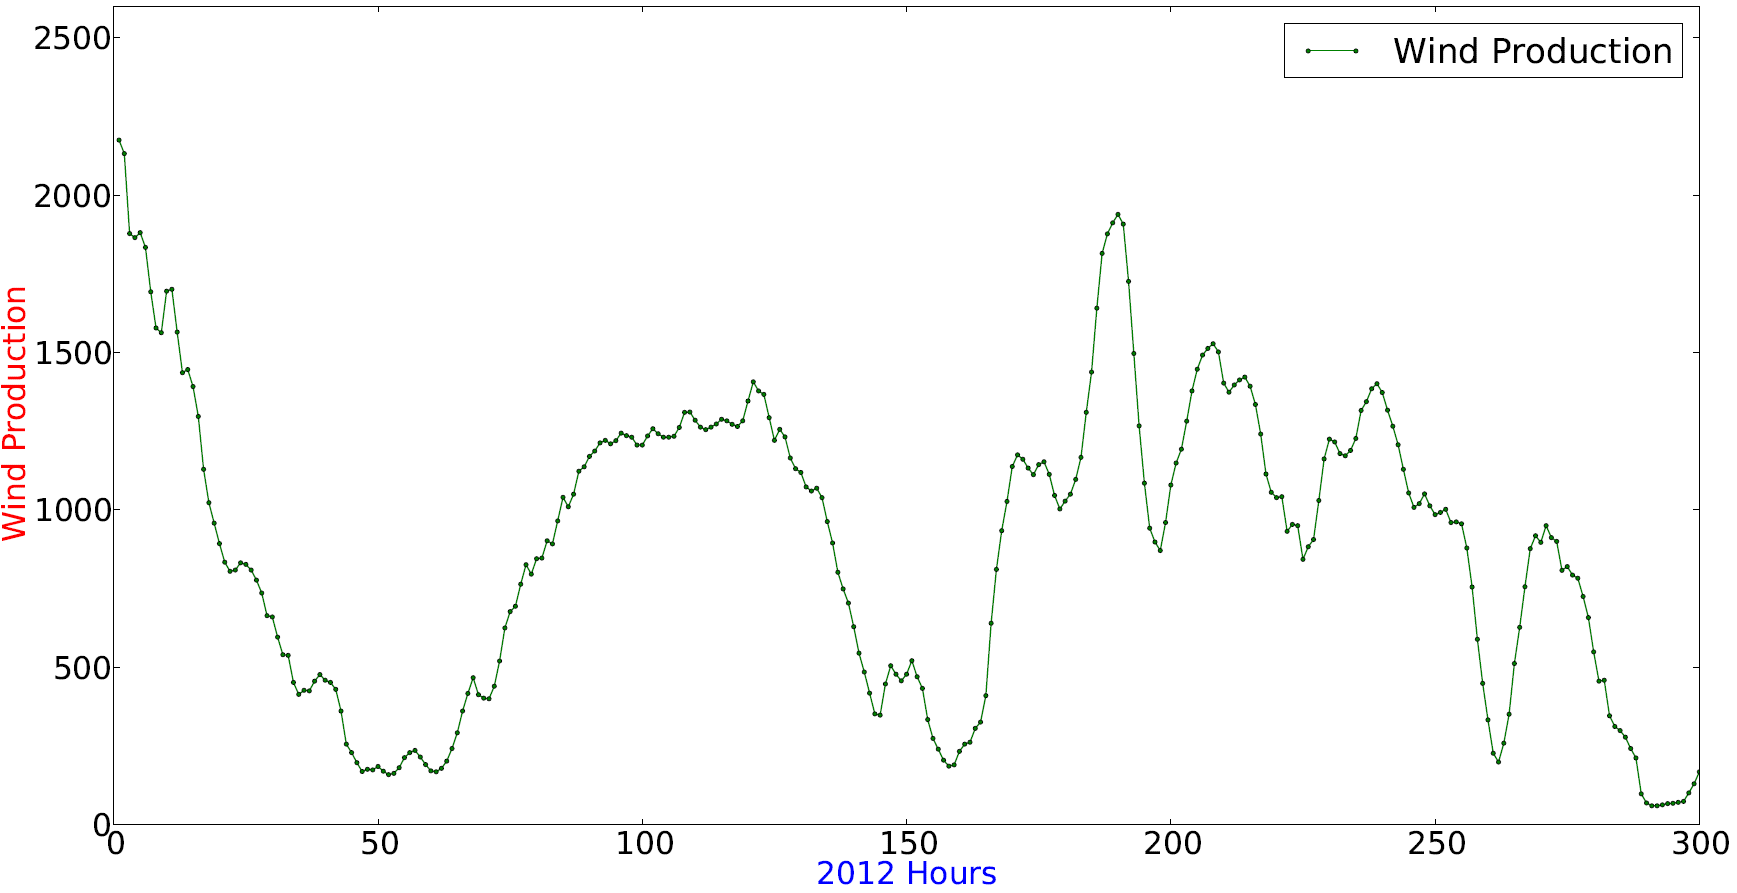
\includegraphics[width=0.99\linewidth,natwidth=898,natheight=587]{billeder/productionTendency400Hours.png}
\caption{Wind production development for 400 hours in 2011}
\label{fig:windHourDevelopment400Hours}
\end{figure}

\begin{figure}[H]
\centering
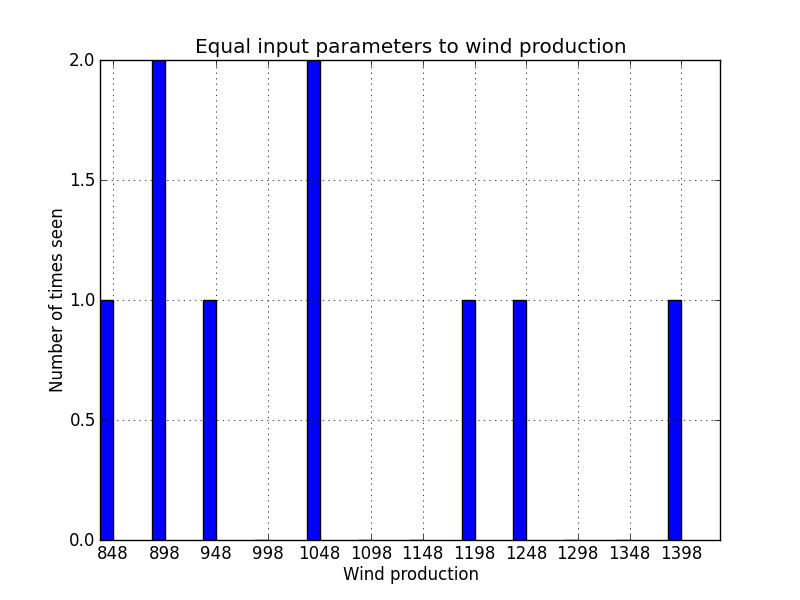
\includegraphics[width=0.99\linewidth,natwidth=898,natheight=587]{billeder/Equal_wind.png}
\caption{Same input parameter to wind production output distribution}
\label{fig:inputParameterDistribution}
\end{figure}

\begin{table}[H]
\centering  % used for centering table
\begin{tabular}{c c c c} % centered columns (3 columns)
 & \#1 Windspeed & \#2 Temperature (Celsius) & \#3 Demand \\ [0.5ex] % inserts table 
%heading
\hline                  % inserts single horizontal line
High margin: & 16.5 & 3.3 & 2359.5  \\
Low margin: & 13.5 & 2.7 & 1930.5 \\ [1ex] % [1ex] adds vertical space
\hline %inserts single line
\end{tabular}
\caption{This is the high and low margins used for the the similar input to output distribution.} % title of Table
\label{table:similarHoursLimitsWindProd} % is used to refer this table in the text
\end{table}

\todo{price irregular price curves - it does not make sense to trim in the case of wind production because it does have irregularities that is unpredictable or at least does not make sense as seen in price. By doing this would wound break the curve and could potentially remove important data for the generalization function}

Figure~\ref{fig:windHourDevelopment400Hours} does not show any need for trimming when predicting wind production. The curve of wind production does not contain any cases that are unpredictable, e.g productions that suddenly drops without any intermediary steps. \todo{Explain better!!}.

\todo{Find graph and tell something about the general movements of the wind production. Further more show it together wind wind speed - should see coherence. Use this to locate the irregularities where it does not hold at all}
\todo{write something about that we need to look back}

\todo{In the experiments show a graph of why we add the curve analysis. The network itself tries to do a general fit and because the same input parameters can point to a interval of price/production we need to give the prediction a kind of "snapshop" of the current situation so that it knows which way to go based on the current market situation - we give it more information to base its decision on - if the current input parameters can point to a price between 700-1100 but the price from one hour ago was 900 and the current trend from the last 24 hours is going up then we should probably not guess below 900 - we don't know but since we otherwise would random an answer, the probability of trusting statistics is better. By doing this we can better approach our target to predict}

\todo{GENERATION HOURS}

\section{Electricity Price Analysis}
\label{sec:ElectricityPriceAnalysis}
Energy price prediction is a cumbersome task to handle because of the highly volatile nature of price prediction and the plethora of factors that influence the energy price. In this section we will show the factors that influence the price by analysing relevant data that will later become input in our ANN. Not to surprisingly; the most important factor in any market is demand and this greatly influences the price "REFERENCE". But also time of day, day of the week, wind speed and temperature (which are the quantifiable factors) play a big role. Sociocultural influences affects the price aswell but are hard to measure. This section will show the connection between energy price and some of the influential factors.

%Table ~\ref{table:pearsonCoeficientPrice} shows the correlation coefficient between factors that have been discussed earlier as having an influence on the electricity price. As discussed in the wind production section the correlation coefficient is a value between -1 and +1 that represents the linear dependency between two variables. 

%\begin{table}[H]
%\centering  % used for centering table
%\begin{tabular}{c c} % centered columns (3 columns)
%Input factor \#1 & Pearson Correlation Coefficient \\ [0.5ex] % inserts table 
%heading
%\hline                  % inserts single horizontal line
%Consumption & 0.281301381724 \\ % inserting body of the table
%Wind Speed & -0.271821873508 \\
%Temperature & -0.147262088023 \\
%Wind Direction & -0.161895363332 \\ [1ex] % [1ex] adds vertical space
%\hline %inserts single line
%\end{tabular}
%\caption{Table showing Pearson correlation coefficient between various factors and the price.} % title of Table
%\label{table:pearsonCoeficientPrice} % is used to refer this table in the text
%\end{table}

\subsection{Price}
We present some of the influences on the price in this section and argue why these parameters has an impact on the price. We also account for the time perspective of the price and show the non-linear nature of energy prices. Since we just talked about demand and the influence on price we will here be focusing on the other impacting factors in the prediction of energy prices. To accompany the graphs we also calculated the Pearson's correlations (section ~\ref{sec:Pearsons}) which can be seen in table ~\ref{table:pearsonsPriceVariables}.

Pearson's correlations:
\begin{table}[!ht]
\centering  % used for centering table
\begin{tabular}{c c} % centered columns
 \#0 Parameters & \#1 Pearsons \\ [0.5ex] % inserts table 
%heading
\hline                  % inserts single horizontal line
Price/Demand & 0.310686748459 \\
Price/Wind speed & -0.278480552449  \\
Price/Temperature & -0.175026569339 \\
Demand/Wind speed & 0.567853517055 \\
Demand/Temperature & -0.592827186022 \\
\hline %inserts single line
\end{tabular}
\caption{Pearson's correlations for price prediction variables} % title of Table
\label{table:pearsonsPriceVariables} % is used to refer this table in the text
\end{table}

\subsubsection{Weather conditional influences}
The electricity price is affected by different weather conditions. We present temperature and wind speed and show how they influence the price.

\begin{figure}[H]
\centering
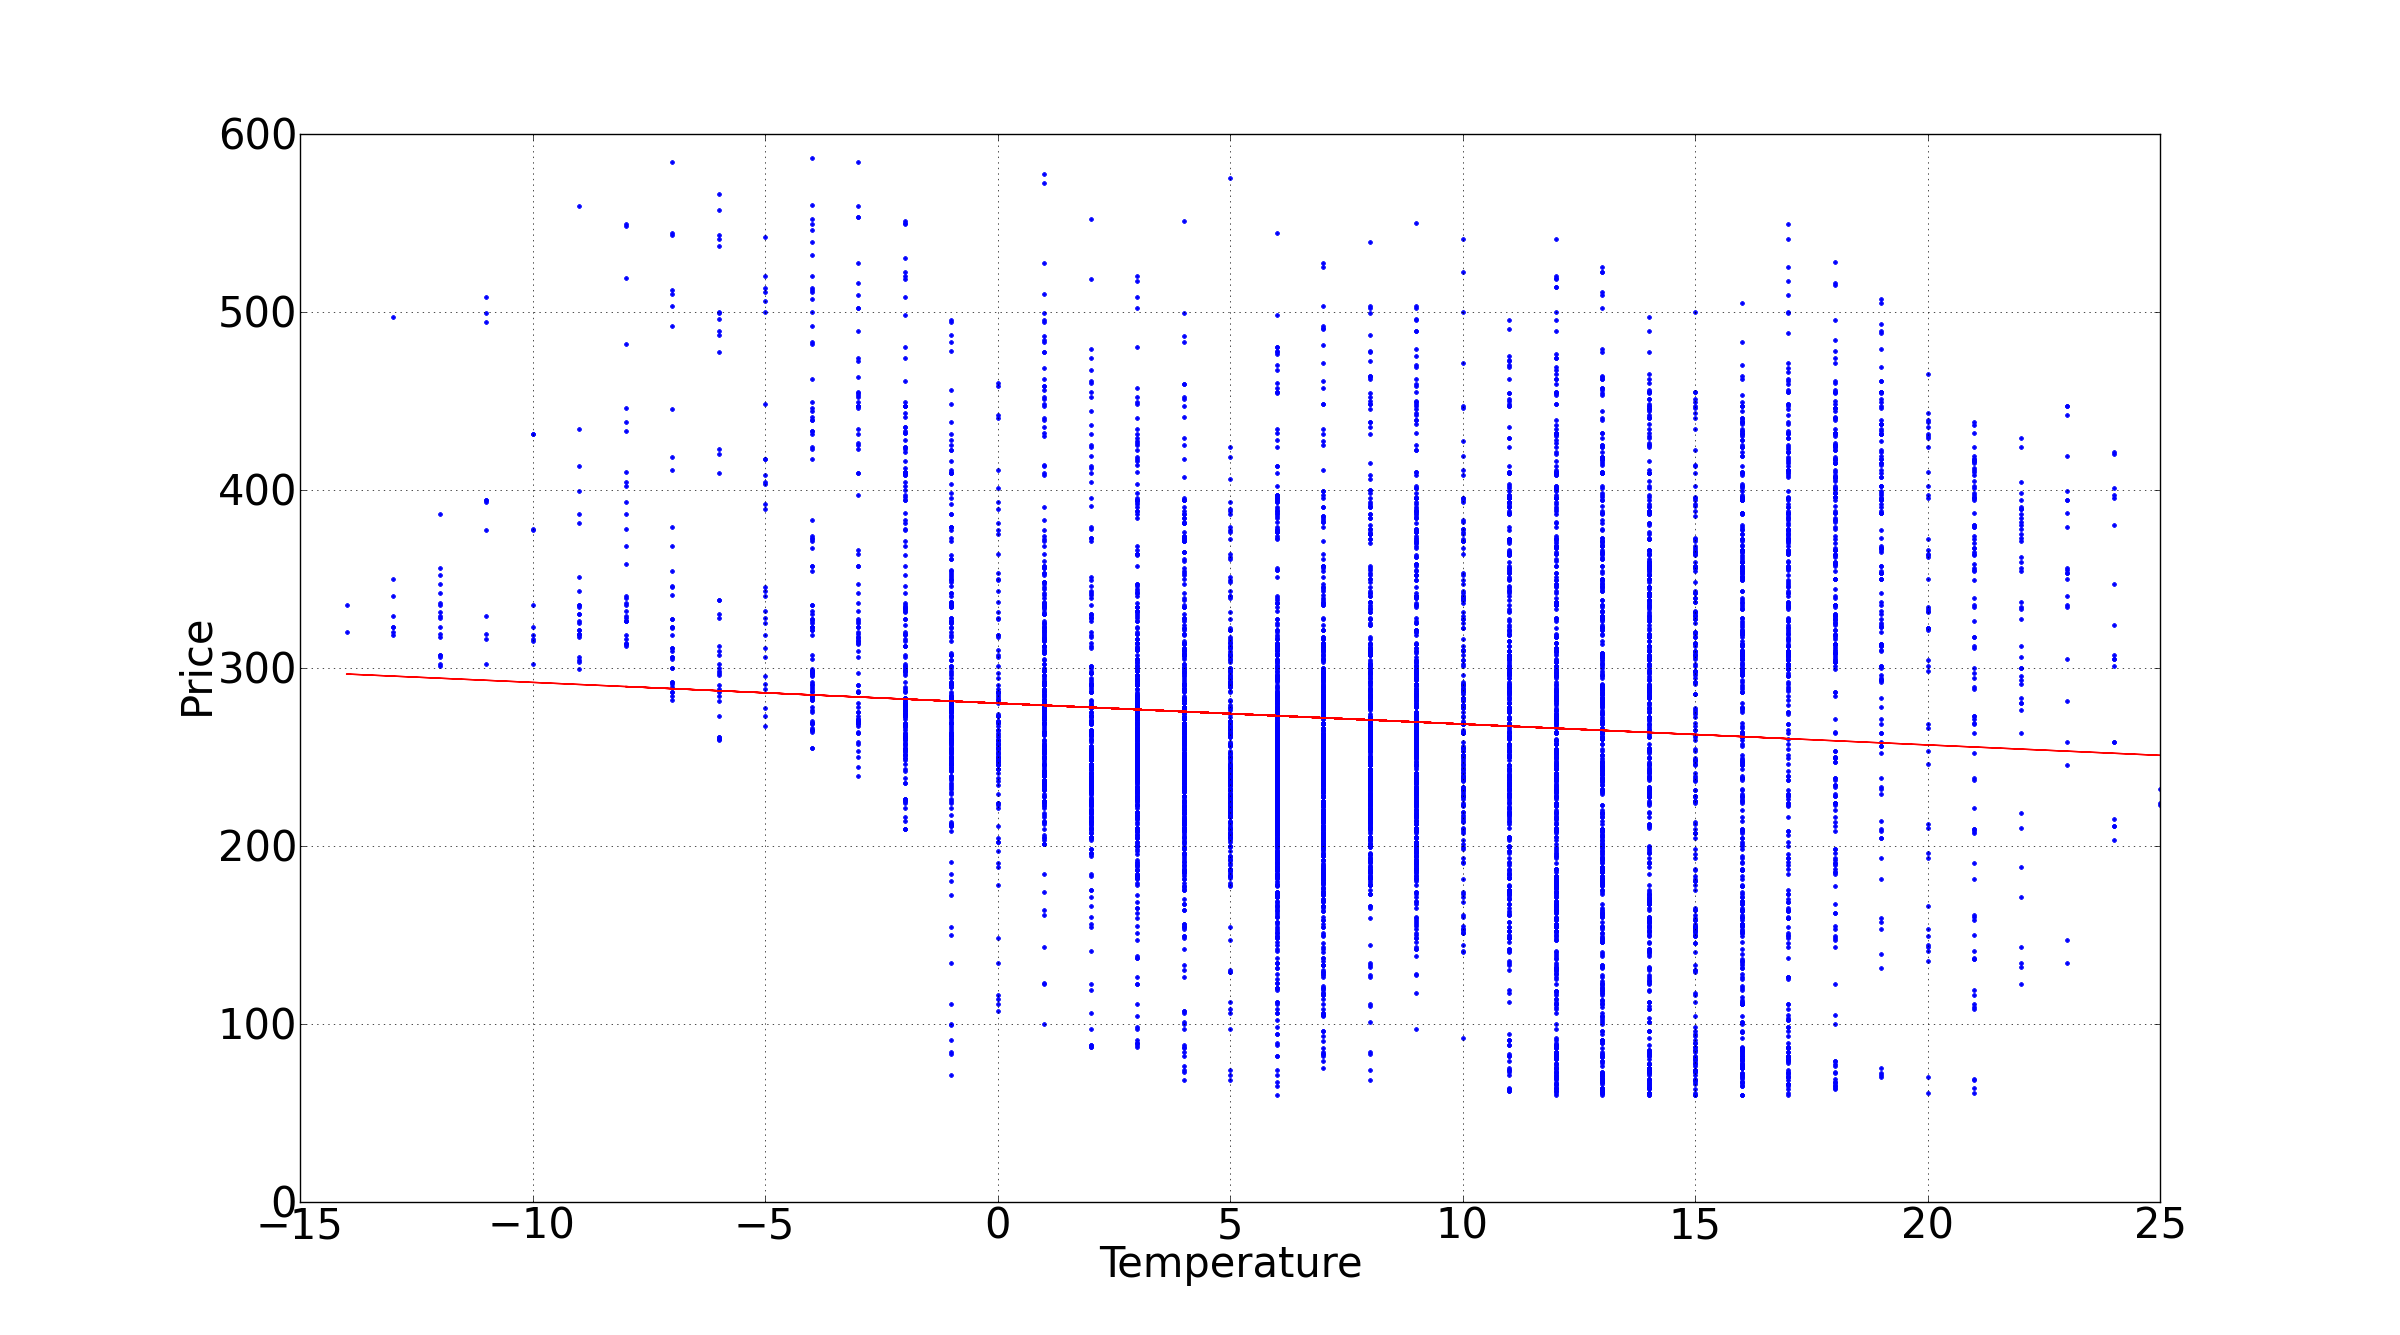
\includegraphics[width=0.8\textwidth ,natwidth=410,natheight=237]{billeder/energy_price_plots/price_temp.png}
\caption{Price and temperature plot.}
\label{fig:price_temp}
\end{figure}

In figure~\ref{fig:price_temp} and table~\ref{table:pearsonsPriceVariables} we see that there is nearly no correlation between temperature and the price. This indicates that we cannot use the temperature as a direct input to the ANN. But the temperature has an indirect influence on the price since it has an influence on the demand. This variable is only used to substitute the demand to make our prediction self-contained. This will be discussed later.

\begin{figure}[H]
\centering
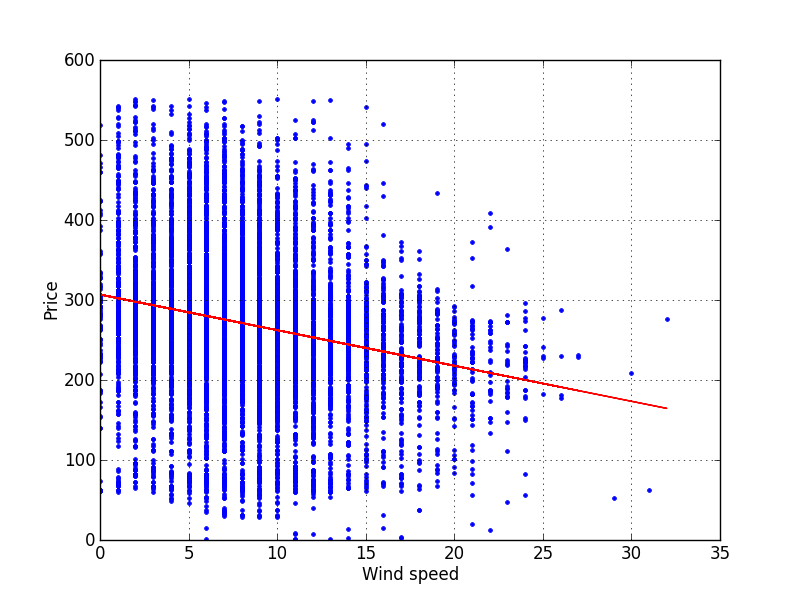
\includegraphics[width=0.8\textwidth ,natwidth=410,natheight=237]{billeder/energy_price_plots/price_wind.png}
\caption{Price and wind speed plot.}
\label{fig:price_wind}
\end{figure}

In figure ~\ref{fig:price_wind} we see how the wind impacts the price. If the wind speed increases the energy price decreases. This is because the wind power production will allow for a bigger output on the general power production. When the production is high and the demand is moderate the price will decrease to get demand up since we cannot store energy for later use. Also wind power production produces nearly 'free' energy when the windmill park is up and running.
\todo{Snak om distributionen. Det skal ikke ses som en 1-til-1, men som en variabel der kan sende prisen i den rigtige retning.}

\subsubsection{Seasonality}
The price is influenced greatly by the seasonality. Seasonality covers the time of year but also the time-of-day and the day-of-the-week in this section. Sesonality plays a significant role in price prediction because the demand is affected by the consumption of the people and since people follow patterns the demand does aswell.

\begin{figure}[H]
\centering
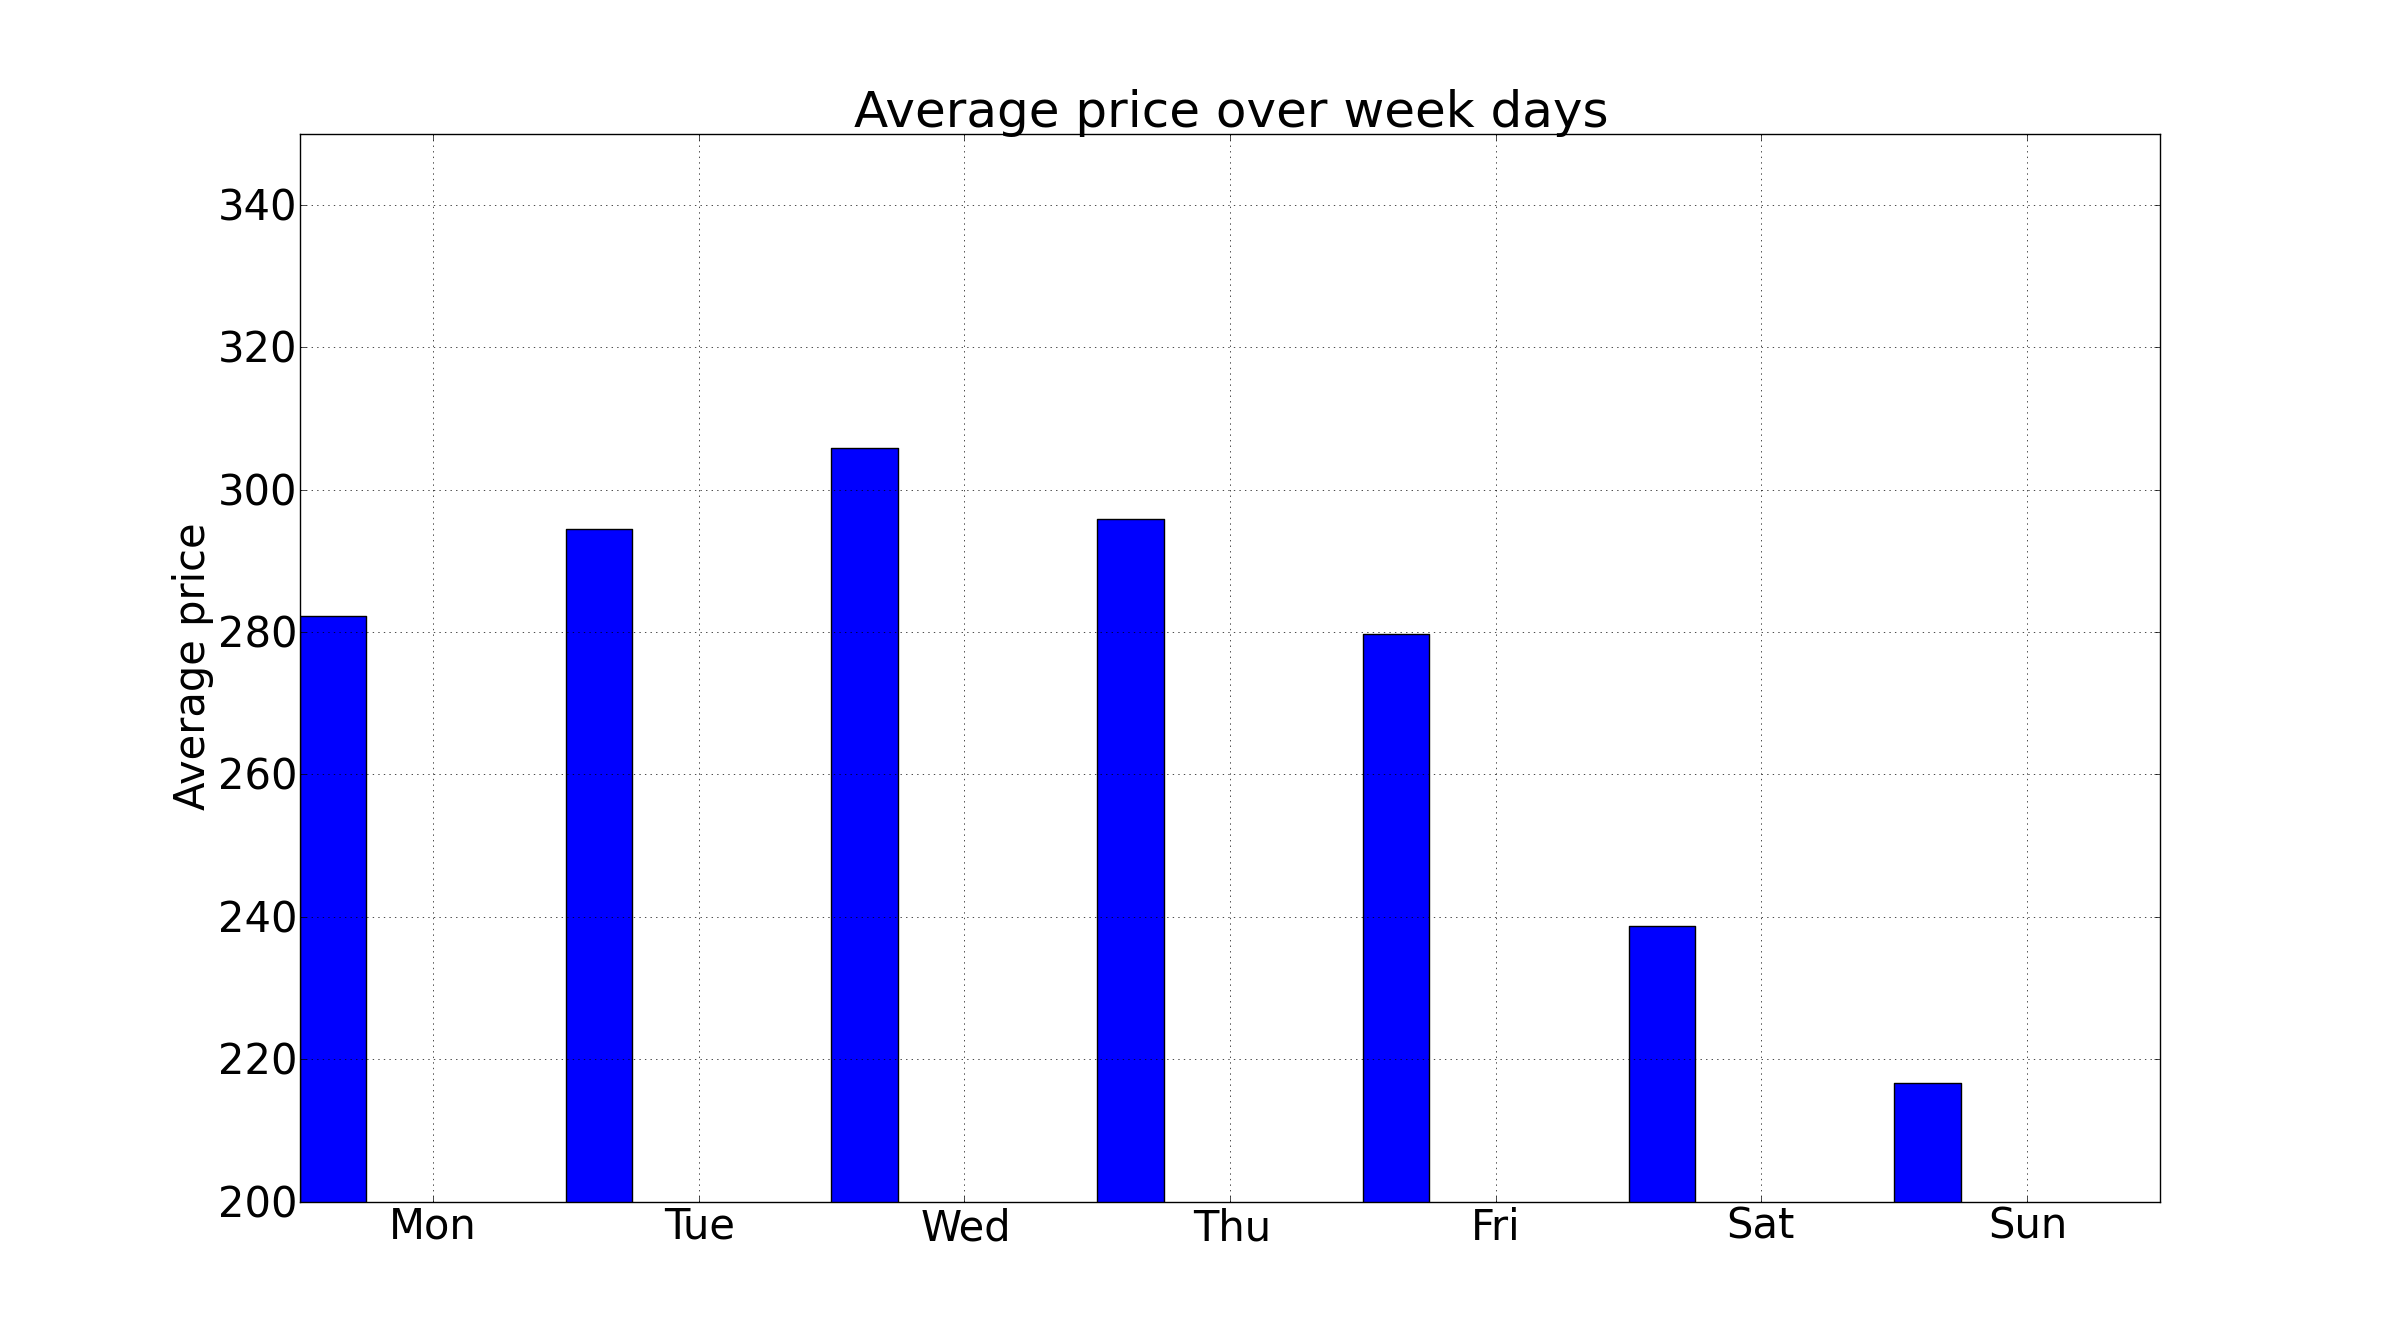
\includegraphics[width=0.8\textwidth ,natwidth=410,natheight=237]{billeder/energy_price_plots/Average_price_over_weekdays.png}
\caption{Daily price dispersion}
\label{fig:price_over_weekdays}
\end{figure}

Figure ~\ref{fig:price_over_weekdays} shows us how the trend of the price varies over the different days in a week. The most noticeable here is how the price is decreasing in the weekend (Saturday and Sunday) and are somewhat steady for the weekdays. We are looking at two options for our neural network. We can represent it as a matrix (section ~\ref{sec:Matrix}) which is the most granulated method. We can also normalize the days 1-7 and represent all days with only 1 input neuron.
The graph show us a difference between highest (Wednesday) and lowest (Sunday) of 80 which is pretty much when the price fluctuates between 632 and 61 (with 1\% top and bottom trim see section ~\ref{sec:Trimming}).

\begin{figure}[H]
\centering
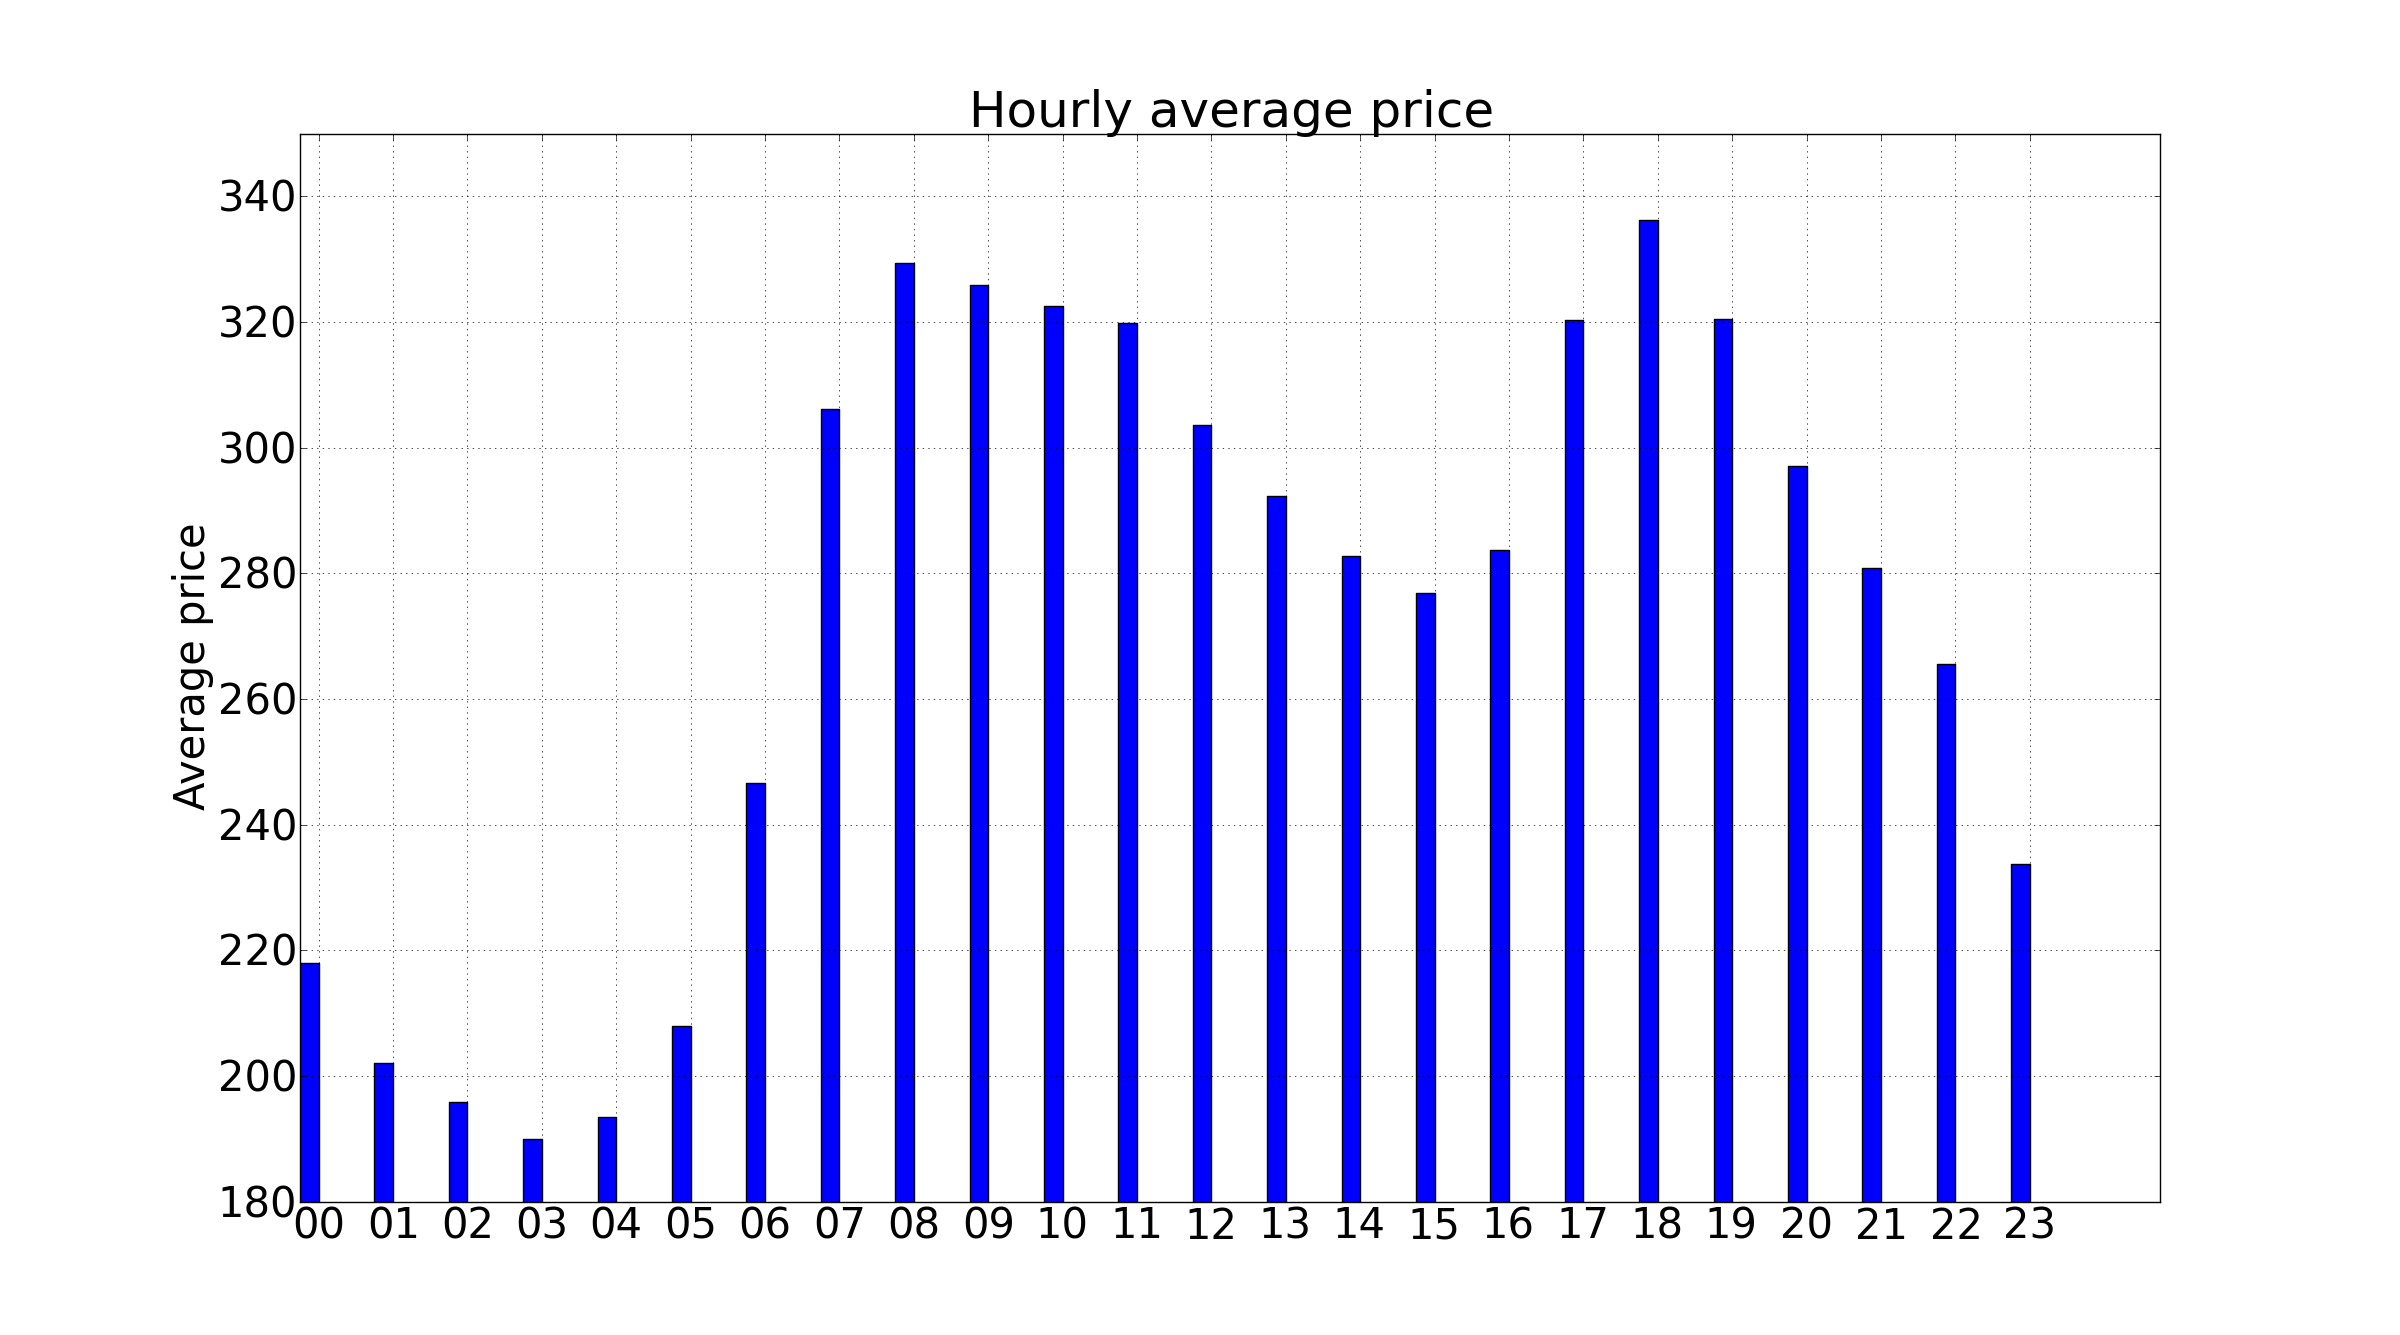
\includegraphics[width=0.8\textwidth ,natwidth=410,natheight=237]{billeder/energy_price_plots/price_per_hour.png}
\caption{Hourly price dispersion}
\label{fig:price_per_hour}
\end{figure}

In ~\ref{fig:price_per_hour} we see the average price per hour over a whole day. We see a trend where the price is highest from 08 to 10 and again from 17 to 19. This is because most people wake up in the first interval and use a lot of electricity and the second interval is when everybody gets home and cooks dinner. The price can be represented (as described in price-over-weekdays) as a matrix or a single normalized input. The price fluctuates between 335(18) and 190(03) which gives us a difference of 145. This is a pretty significant difference between highest and lowest and will help us point the prediction in the right direction.

\begin{figure}[H]
\centering
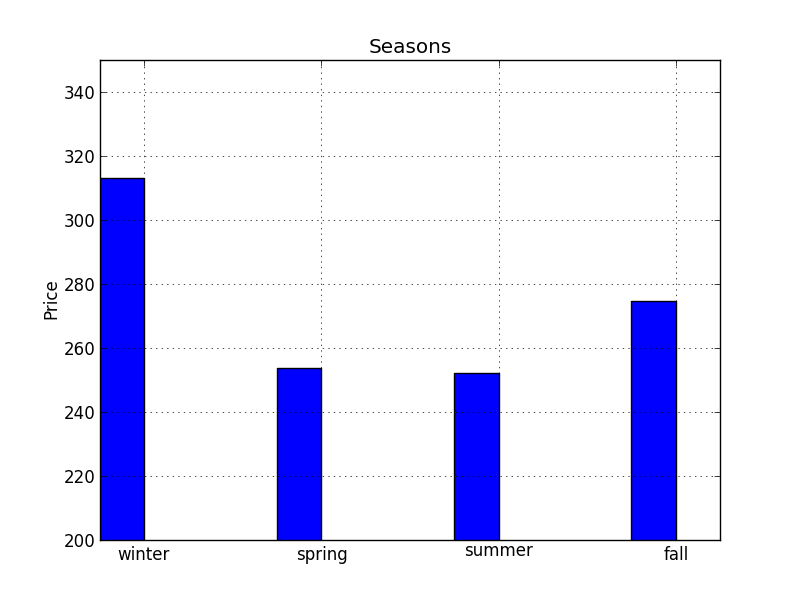
\includegraphics[width=0.8\textwidth ,natwidth=410,natheight=237]{billeder/energy_price_plots/seasons.png}
\caption{Seasonal price dispersion}
\label{fig:seasons}
\end{figure}

The sesonality is also reflected in what time of year it is. In the winter time the electrical heating and need for electric light plays a significant role on how much electricity is consumed and thus the price goes up. This is shown in figure ~\ref{fig:seasons} where it clearly shows the average price is higher in winter and fall than in summer and spring.

\begin{figure}[H]
\centering
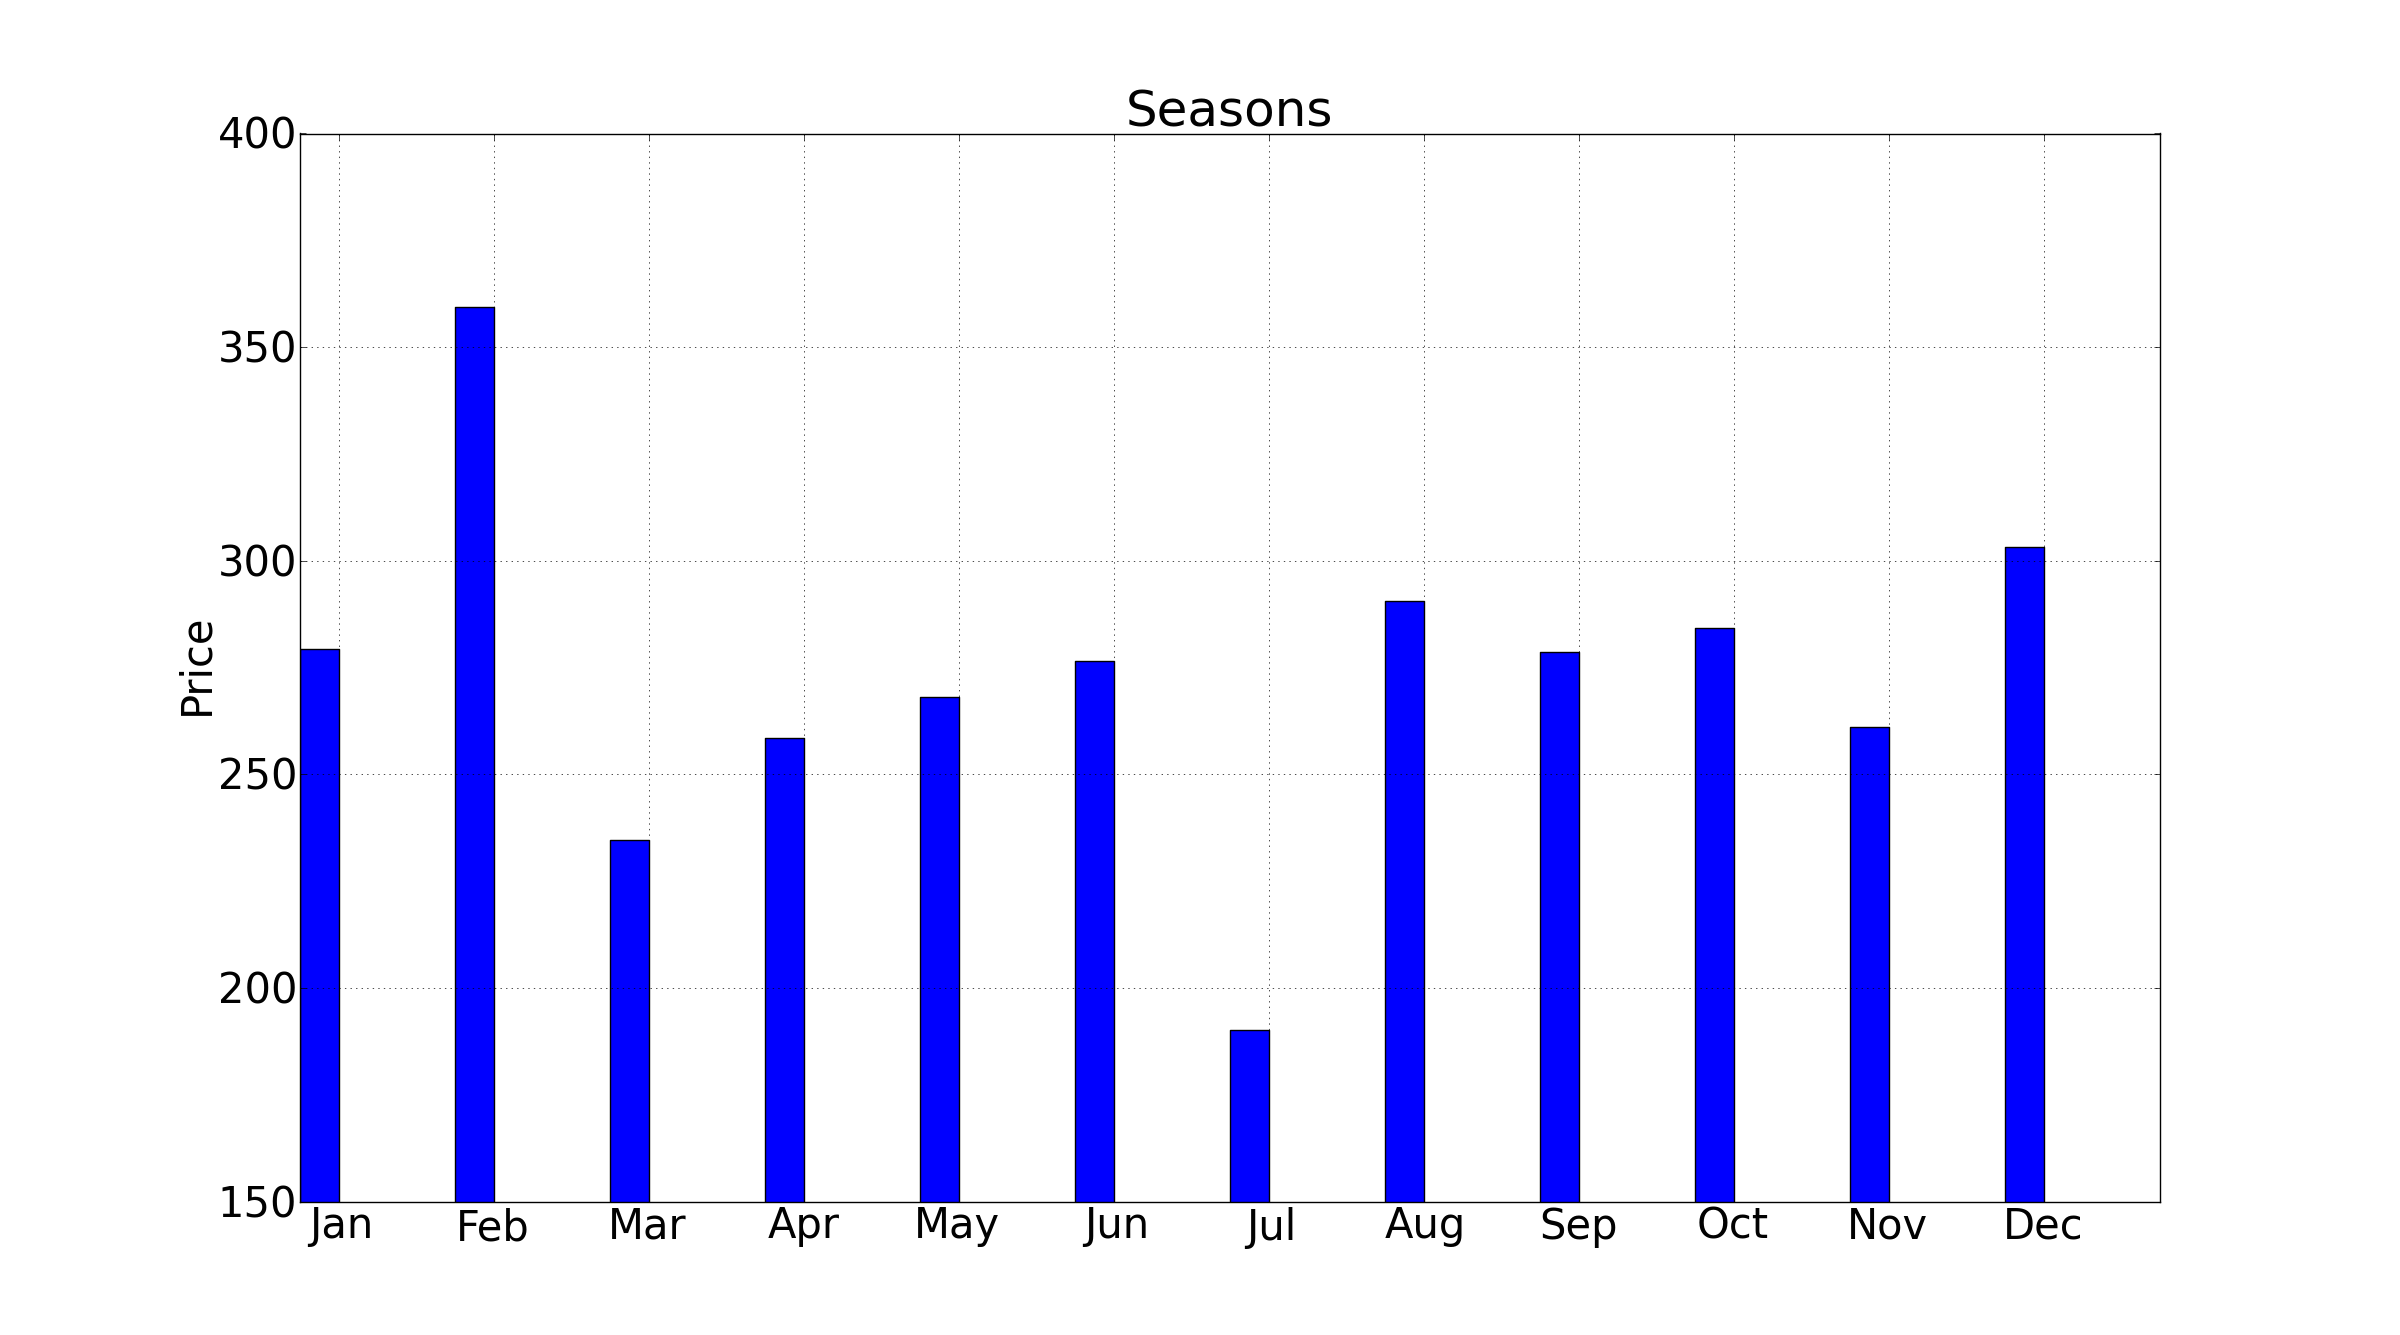
\includegraphics[width=0.8\textwidth ,natwidth=410,natheight=237]{billeder/energy_price_plots/averageMonthlyPrice.png}
\caption{Monthly price dispersion}
\label{fig:monthlyAveragePrice}
\end{figure}

To get a more fine grained representation of the seasonal influences on the price; we created a monthly distribution of the price. The figure ~\ref{fig:monthlyAveragePrice} shows that the highest average price is 360(february) and lowest 190(july). This is a significant price jump and shows the same trend as for the seasonal figure ~\ref{fig:seasons} but here we see the effects of the holidays in july; where the price is significantly lower than the rest of the year.

\subsubsection{Volatility and High-Frequency}
The energy prices are very volatile and changes on an hourly basis. The volatility is often reflected in the same conditions for the hour gives completely different results. In addition to the volatility the price has a very high frequence of spike prices. A spike price is a price that elavates very quickly and drops in a matter of a few hours. These conditions can be tricky to handle but we will here address some of the problems in handling volatility and spike prices.

\begin{figure}[H]
\centering
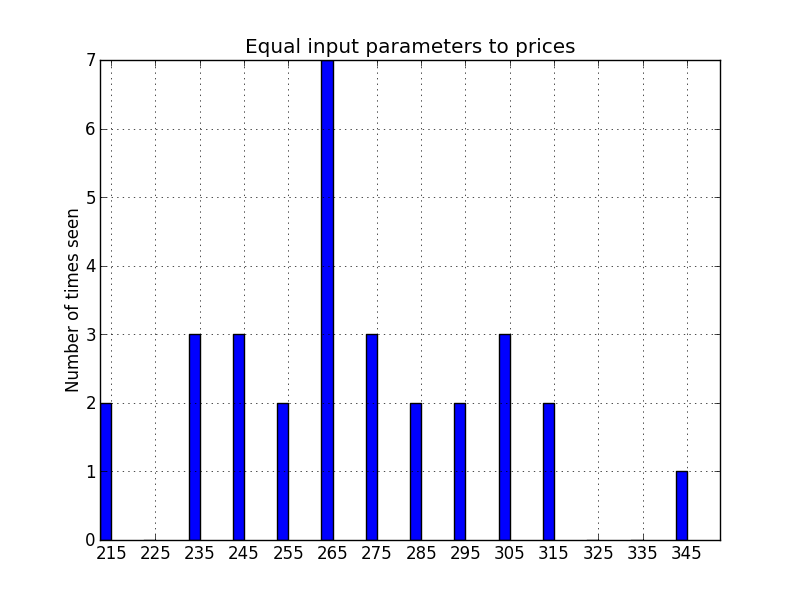
\includegraphics[width=0.8\textwidth ,natwidth=410,natheight=237]{billeder/energy_price_plots/same_hour_distribution.png}
\caption{Price ditribution over equal hours}
\label{fig:same_hour_distribution}
\end{figure}

In earlier figures we have shown how the input influences the price and given some reasons to why this influences the price. In figure~\ref{fig:same_hour_distribution} we have chosen similar hours across all days of a year and we show how different the price can be for similar inputs. The similar days have been chosen from the 'core' inputs (wind speed, temperature and demand) and the margins seen in table~\ref{table:similarHoursLimits} reflects the upper and lower bound of the inputs. The margins are calculated from a randomly chosen day and the interval is 10\% up and down. Even though the price is volatile we can see a trend in the graph that shows us that the price most of the time will be about 265.

\begin{table}[H]
\centering  % used for centering table
\begin{tabular}{c c c c} % centered columns (3 columns)
 & \#1 Windspeed & \#2 Temperature & \#3 Demand \\ [0.5ex] % inserts table 
%heading
\hline                  % inserts single horizontal line
High margin: & 12.1 & 6.6 & 2510  \\
Low margin: & 9.9 & 5.4 & 2053 \\ [1ex] % [1ex] adds vertical space
\hline %inserts single line
\end{tabular}
\caption{This is the high and low margins for our similar hours comparison.} % title of Table
\label{table:similarHoursLimits} % is used to refer this table in the text
\end{table}

\begin{figure}[H]
\centering
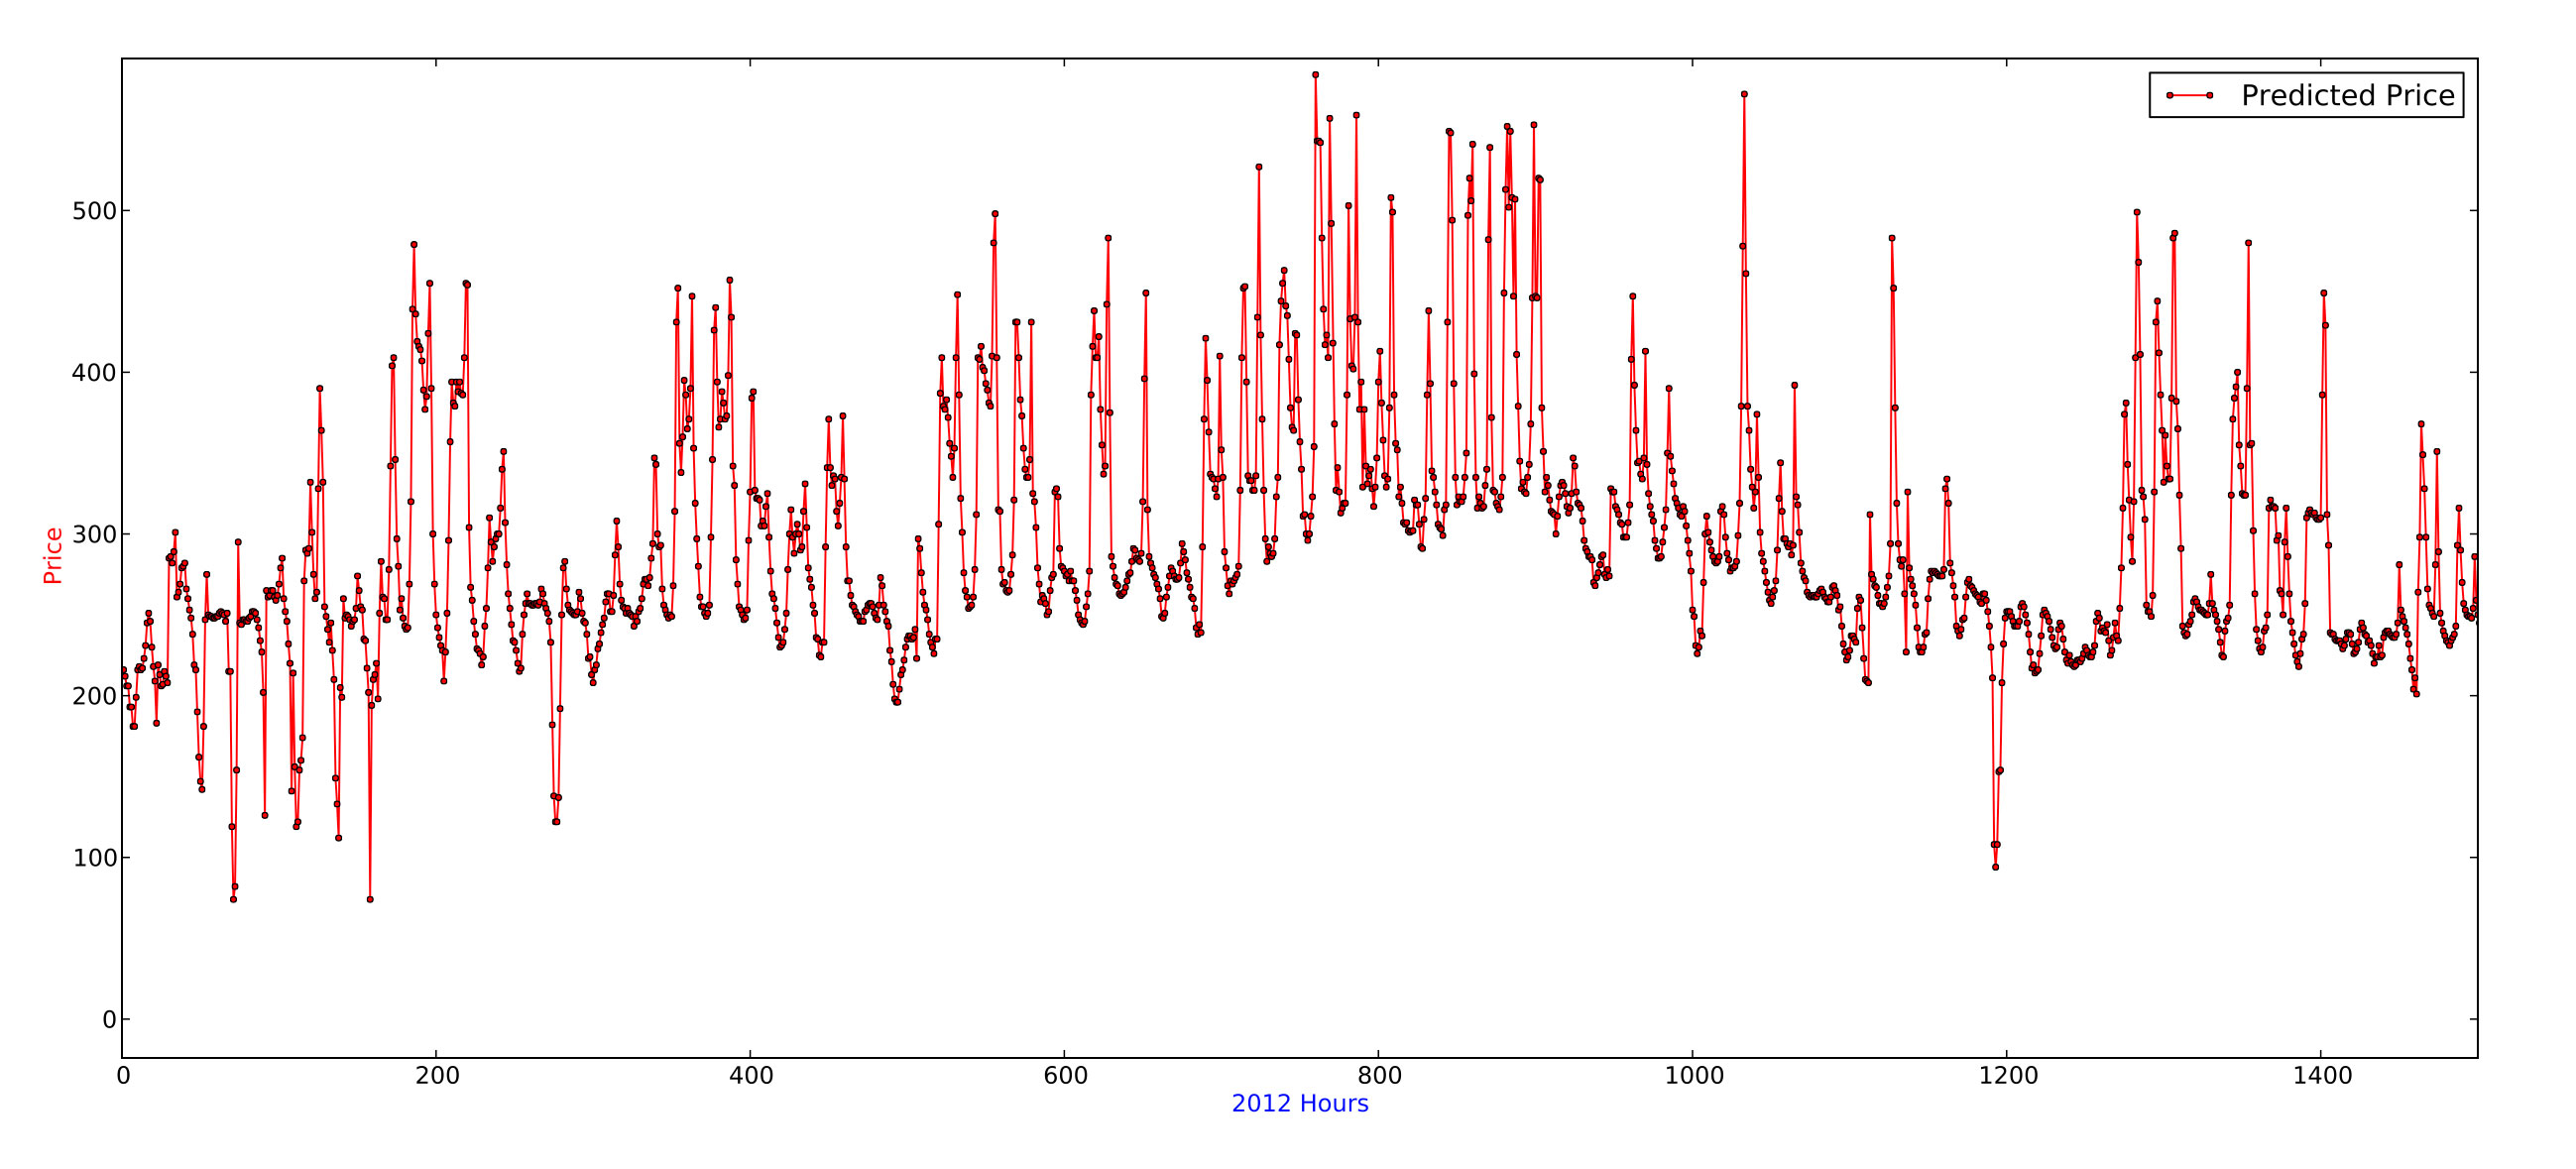
\includegraphics[width=\textwidth ,natwidth=410,natheight=237]{billeder/energy_price_plots/plotGraph.jpg}
\caption{A plot graph of the price development over the first 1500 hours in 2012}
\label{fig:plotGraph}
\end{figure}

The volatility of the price is clearly shown in~\ref{fig:same_hour_distribution} where the price on similar hours fluctuates from 215 to 345. To address the volatile nature of the price we need to look at the trends of the known historical price. If we take a look at the price plot in figure~\ref{fig:plotGraph} it clearly shows how volatile the price actually is. Another thing we can derive from the graph is how the price moves. It doesn't just jump from top to bottom of the interval but it takes some steps to get there (in most cases). This tendency can be used alongside the last known price to give the neural network a direction to follow and an approximate price as a point of origin. For more details on this see section~\ref{sec:usingStatisticalInput}. As an example we can take a price of 250 and a rising tendency then we have pointers for the price development and we can in general discard every posibility of a price that is under 250 -- since the tendency was rising. We can also discard the highest of numbers since the price in general doesn't jump several hundred and therefore we will have an idea of where the price is heading even though it is very volatile.

In the same manner we can address the high-frequency spike prices that occurs in the time series. We have to identify a tendency in the historical data and use this to make the predictions follow the steep spikes in the dataset. The volatility is often easier to handle than the spike prices because the volatility most of the times only causes small jumps in the price and these are easier to predict.

\subsubsection{Demand}
Demand is directly connected to the energy prices (which comes as no suprise) since every market is driven by demand. Since demand is relative to the present time we are not able to use it directly as an input factor in the artificial neural network(ANN). We have a couple of choices here. We can take the demand from other instances like Nord Pool Spot; where they predict what the demand will be. We can compute the demand in artificial neural network and use the outputs as input for our price prediction ANN. At last we can try and substitute the demand input with the factors that plays a role in predicting the demand. The last two methods requires us to have an idea of what the input parameters for the prediction of demand is. As mentioned in related work we have seen a function that calculates the demand based on CDD(Cooling degree days), HDD(Heating degree days), ELD(Humidity), V$_w$ (Wind speed), M$_s$ (Sunshine), M$_r$ (Rainfall) \cite{19}. Based on this we will model the ANN to take the above mentioned factors as inputs.

\begin{figure}[H]
\centering
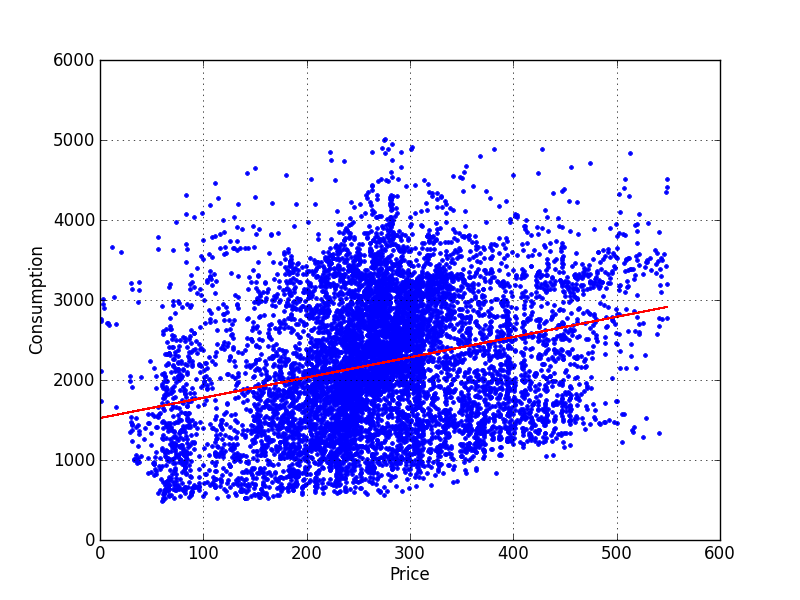
\includegraphics[width=0.8\textwidth ,natwidth=410,natheight=237]{billeder/energy_price_plots/consump_price.png}
\caption{Demand and price plot.}
\label{fig:consump_price}
\end{figure}

In figure ~\ref{fig:consump_price} we see the connection between energy price and the demand. The model shows us that if the demand rises the price on the energy rises aswell. This is a common tendency in a market where there isn't endless supply. Since the price is heavily influenced by demand and demand is a relative factor the same calculations are also done by the powerplants because they need to know how much power to produce in a certain timeframe. We want to imitate this forecast and predict our own demand based on the aforementioned parameters. This is key to how accurate we will be able to predict the price. In other words: A good prediction of the demand will give us the right foundation for a good prediction of the price.

\begin{figure}[H]
\centering
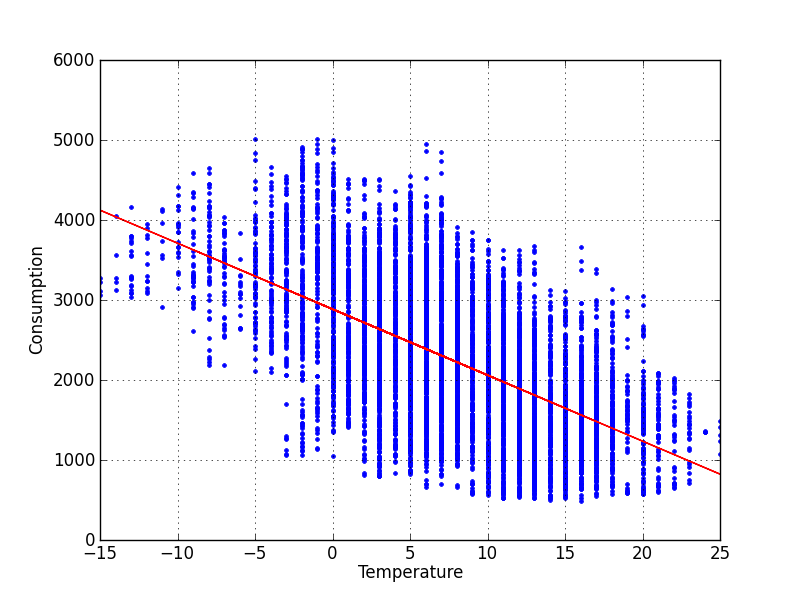
\includegraphics[width=0.8\textwidth ,natwidth=410,natheight=237]{billeder/energy_price_plots/consump_temp.png}
\caption{Demand and temperature plot.}
\label{fig:consump_temp}
\end{figure}


In figure ~\ref{fig:consump_temp} we see the connection between demand and temperature. The temperature itself has an influence when it is very cold or very warm. This connection is expressed as CDD and HDD. In figure ~\ref{fig:consump_temp} we see that if temperature decreases the demand will go up. This is presumably because the people of Denmark use a lot of energy on heating their homes and lighting them in the winter time. In \cite{19} they also describe CDD which indicates the need for cooling. In Denmark it is limited how high the temperature goes and how often we actually need to cool our homes.

\todo{Create the CDD and HDD graphs}

\begin{figure}[H]
\centering
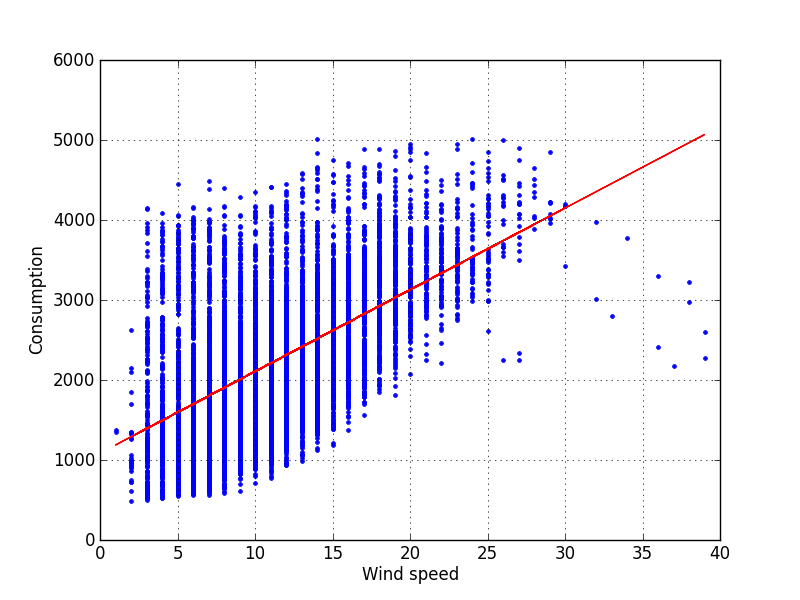
\includegraphics[width=0.8\textwidth ,natwidth=410,natheight=237]{billeder/energy_price_plots/consump_wind.png}
\caption{Demand and wind speed plot.}
\label{fig:consump_wind}
\end{figure}

Wind speed plays a role in predicting electrical demand. The wind affects the electrical heating needed in homes across the country. The wind cools down the houses and thus need for heating arises \cite{19}. As seen in figure ~\ref{fig:consump_wind} and in table ~\ref{table:pearsonsPriceVariables} there is a pretty good correlation between wind speed and consumption. The graph clearly shows us that; when the wind speed increases (from 15 and up) the overall demand increases aswell. This indicates that high wind speeds will have th greatest influence on the demand.

\section{Discussion}
The analysis of the electricity price and the wind power revealed similarities between the two and correlations between input data and the wind power/electricity price that was surprising.

First of all, the demand was expected to influence electricity price but not the wind power as significantly as we established. The expectation was that \fnurl{Nord Pool Spot}{http://www.nordpoolspot.com/} would only influence the market and not the other way around \fnurl{wind power}{http://en.wikipedia.org/wiki/Wind_power_in_Denmark\#Capacities_and_production}. The connection indicates that the wind power is moved into the electricity market according to the demand.

The timely and seasonal factors showed to have an influence on the electricity price (Section \ref{sec:seasonality}) and the wind power(Section \ref{sec:windProdSeasonality}). The demand influence price and since demand is much controlled by consumer habits these will be reflected in the price. Wind power surprisingly showed a pattern in time of day productions due to the established connection to demand. The seasonal factors also showed an impact on both datasets. The wind power is influenced greatly by wind speed which reflects the seasonal changes in the meteorological factors. The price is affected by seasonal changes in the demand for electric use which are also because of the meteorological factors thus solidifying that meteorological factors plays a great role when determining wind power and electricity price forecasts.

Another factor that had a great influence was the last-known price(Section \ref{sec:Price}) and wind production(Section \ref{sec:windProductionDev}). This shows that the behaviour of the curve is important when we are predicting either wind power or electricity prices. If we are able to know the exact price/wind production before the one we are trying to predict the predictions could possibly obtain better accuracy due to the strong correlation to the last known value. This can be a challenging task when performing day-ahead prediction because all steps must rely on all previous predictions (except from the first hour). We will examine different approaches. 

We saw that volatility played a role in both of the datasets but with more significance for the electricity price. The volatility for price can be explained by the sociological factors as mentioned in Section \ref{sec:volatility} that are very hard to foresee because of their unpredictable nature. These factors can also be play a role for wind power since it is affected by the demand. Accounting for these factors in the network model is necessary to investigate because it will help add further characteristics of the price or wind power.

%Also talk about differences and similarities in the two data sets. Same data. Seasonality and hours impact both. ect.
%Demand i forhold til wind speed. Større link imellem markedet og vindkraft.
%Time of Day spiller ind paa begge to. Maaske surprising at den ogsaa har indvirkning paa wind power.
%Seasonality i forhold til de to.
%High correlation between last-known input and the price to predict.
%Volatilility i begge. Price mest.

%%%%%%%%%%%%%%%%%%%%%%%%%%%%%%%

\chapter{Forecasting Model}
\label{ch:forecastingModel}
\section{Artificial Neural Network Overview}
This section will give a short overview of the applied network pattern and the learning algorithm used for training of the network. The overview will be based on the more detailed explanation in Section~\ref{sec:annSection}.

\subsection{Structure}
Feed-forward will be the preferred architecture for predicting the electricity prices and wind power productions in this thesis. It is the most common structure and data flows from the input to the output layer through the hidden layers in between. The input layer will consist of all the the influential factors of wind power or electricity price and the output will be the predicted price or wind power. Figure~\ref{fig:overviewAnn} illustrates the concept well.

\begin{figure}[H]
\centering
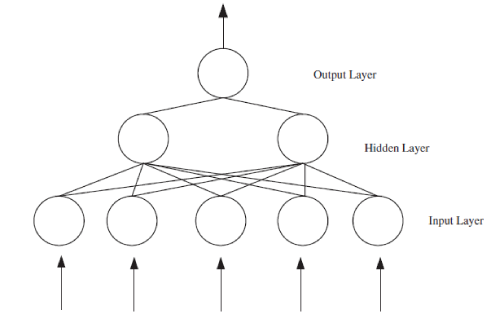
\includegraphics[width=0.8\linewidth]{billeder/ANN.png}
\caption{A simple neural network with 3 layers. \cite{stockForecasting}}
\label{fig:overviewAnn}
\end{figure}

\subsection{Learning}
Training of the network network will be done with the Resilient Back-propagation algorithm. It is faster than standard back propagation \cite{8,15} and is often used with the feedforward architecture which we use here \cite{14,17}. The most significant reason for applying RPROP instead of traditional backpropagation is its performance and the ability to avoid local minima.

\subsection{Framework}
ENCOG
This section will describe what needs to considered when building and modelling the network in terms of actual design and data set manipulation.

\subsection{Neural Network Optimization}
The forecasting models will be implemented using an Artificial Neural Network with back propagation as training algorithm. The network takes as input a time series and in return outputs the predicted value. The success of the network is much dependent on the number of layers, neurons and epochs and the answer is never unambiguous. It is necessary to experiment with different types of numbers in order to find the best match for the problem at hand.

\subsubsection{Layers and Neurons}
We are using a feedforward ANN which is often organized in one input layer, one or more hidden layers and an output layer where each layer has a number of neurons attached\cite{1} - also see Figure~\ref{fig:ANN}. The number of input neurons are equal to the input parameters which also apply for the output layer. 
The complexity arises in the hidden and input layers because a lot of neuron/layer combinations exist. The number of hidden layers and its affiliated neurons is typically chosen by trial and error and then running simulations to find the best fit\cite{1}. The number of inputs for the input layer can be more intelligently selected even though experiments are also needed. This is because the input is related to what actually impacts the output and can therefore often be known before modelling the network, e.g. wind speed has a great influence on wind production and must be included when predicting it.

\subsubsection{Epochs}
The network trains itself in a number of iterations also known as epochs. In every epoch the network is adjusting its weights based on an error measurement that indicates the different between the desired output and the predicted output of the particular epoch\cite{1}. The goal is of course to adjust the weights in enough iterations so that this error measurement becomes as small as possible. This is not necessarily the same as training infinitely will result in the perfect error margin because it can be overfitted as introduced in the Artificial Neural Network section in the Main Concepts chapter. The purpose of the ANN is to generalize beyond the training set and also be accurate on unseen data\cite{1}. The performance of the ANN is therefore to be measured by applying it to a new testing set that has never been seen before.

\subsubsection{Step-ahead forecasting}

\subsubsection{Conclusion}
When modelling the network is necessary to experiment with different types of inputs, hidden layers and neurons to find the best combination. It is also important to consider the number of training  


  EASY TO DO NAIVE

we add a module that will 



do some figures of the network design/model. Also talk about the number of hidden layers must be experimented with to find the best result. - underfit and overfit as well.
TALK ABOUT MULTIPLE-STEP-AHEAD FORECASTING --> see karlbranting
\subsection{Data manipulation}
\label{sec:DataManipulation}
In the following subsections we will describe different strategies for data set manipulation from the most naive approach to more refined approaches such as trimming and analysis. These approaches are applied to the data before sending the input to the network. These strategies are used in experiments with the actual networks to locate the best possible strategy.

\subsubsection{Normalization}
For artificial neural networks to do the best work; the data should be normalized to either bipolar data(-1 to 1) or binary data(0 to 1). This ensures the best performance by the activation functions since the sigmoid activation function has the steepest gradient (see figure ~\ref{fig:Sigmoid}) between -1 and 1 thus giving the finest granulated outputs. The same applies for the hyperbolic tangent(tanh) (see figure ~\ref{fig:Tanh}) activation function. The difference between the two are the output it generates from the same input. The hyperbolic tangent generates output that ranges from -1 to 1 and it has a steeper gradient around the y-axis than the sigmoid function thus giving the tanh function more granulated outputs than the sigmoid function.
\begin{figure}[H]
\centering
\begin{subfigure}{.5\textwidth}
  \centering
  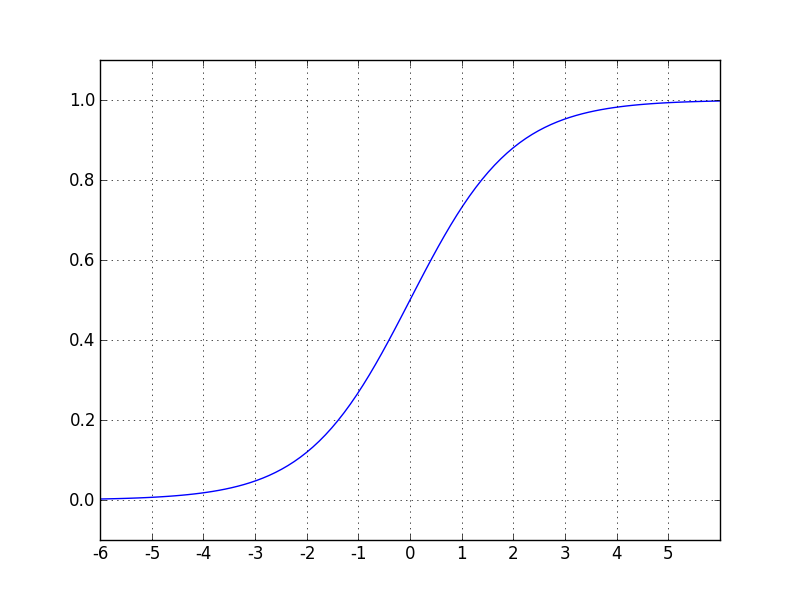
\includegraphics[width=\linewidth,natwidth=898,natheight=587]{billeder/activationFunctions/sigmoid.png}
  \caption{Sigmoid}
  \label{fig:Sigmoid}
\end{subfigure}%
\begin{subfigure}{.5\textwidth}
  \centering
  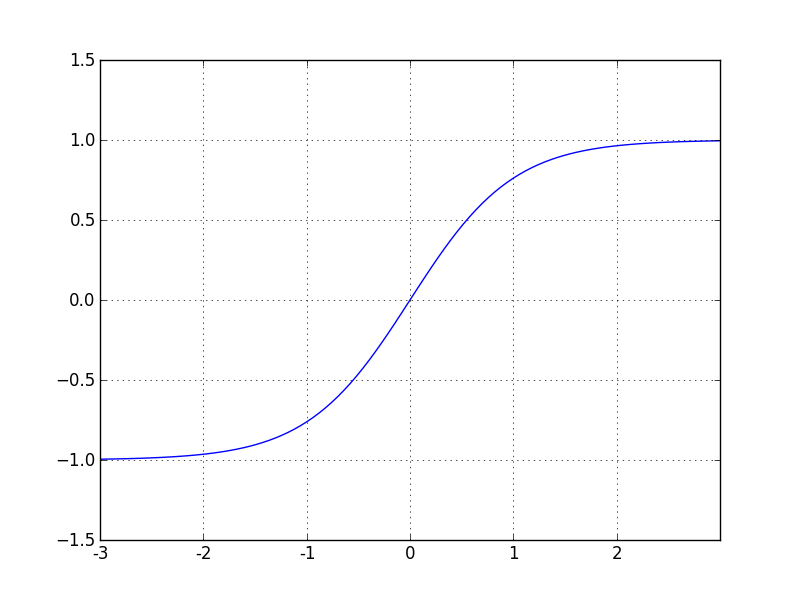
\includegraphics[width=\linewidth,natwidth=898,natheight=587]{billeder/activationFunctions/tanh.png}
  \caption{Hyperbolic tangent(tanh)}
  \label{fig:Tanh}
\end{subfigure}
\caption{Activation functions}
\label{fig:test}
\end{figure}

The normalization of the data is done using the following functions:
\begin{table}[H]
\centering  % used for centering table
\renewcommand{\arraystretch}{2}
\begin{tabular}{c c} % centered columns
 \#Normalization & \#Function \\ [0.5ex] % inserts table 
%heading
\hline                  % inserts single horizontal line
Zero-to-one & $ X_{norm} = \frac{X_i - X_{min}}{X_{max} - X_{min}}$ \\
Minus-one-to-one & $ X_{norm} = \frac{X_i - (\frac{X_{max} - X_{min}}{2})}{\frac{X_{max} - X_{min}}{2}}$ \\
[1ex]
\hline %inserts single line
\end{tabular}
\caption{Normalization functions} % title of Table
\label{table:naiveTrainingApproach} % is used to refer this table in the text
\end{table}
Where $X_i$ is the data entry, $X_{min}$ is the lowest value in the data set and $X_{max}$ is the highest value in the dataset.

\subsubsection{The naive approach}
First of all we tried out the most simple approach available, the naive approach, since this has almost no overhead and takes no preprocessing of the data. The method is simple; you take one neuron per input and one neuron as output. You add all of the data in your training set without doing any preprocessing of data. This kind of training set is good enough for simple problems e.g. the XOR problem or likewise. When we talk about more complex real-world problems like forecasting the energy prices this method does not perform to well and gives less than satisfactory results. Another factor is that a huge part of getting a neural network to perform well is the manipulation of the dataset to get rid of outliers and some of the noise in the dataset. Nevertheless it still gives an indication whether you have some kind of coherence between your input data and the output data even though the results are less than satisfactory. \todo{Mere generelt}

\subsubsection{Trimming}\label{sec:Trimming}
As mentioned before we need to get rid of some of the outliers and some of the noise in the data set to make it easier for the network to approximate a function based on the input data. There are different approaches to trimming but the two we use are standard trimming and percentile trimming of the dataset. Standard trimming is a simple way of getting rid of the worst outliers. The way to do it is; take a low and a high number in your data set and remove everything below and above these limits. Of course this can be very arbitrary but with a simple plot diagram you will be able to see where the limits should be set. Percentile trimming is a statistic approach where you remove the x\% of the dataset from the top and the bottom. You make a percentwise distribution over your dataset; starting with the lowest values in the beginning and ending in the highest values. You calculate the 5th percentile which represents the lowest 5\% of your dataset and then remove these values. The same is done for the top 5\% which results in the removal of the most extreme outliers and has made your dataset less error prone when statistical analysis on it.
\begin{figure}[!ht]
\centering
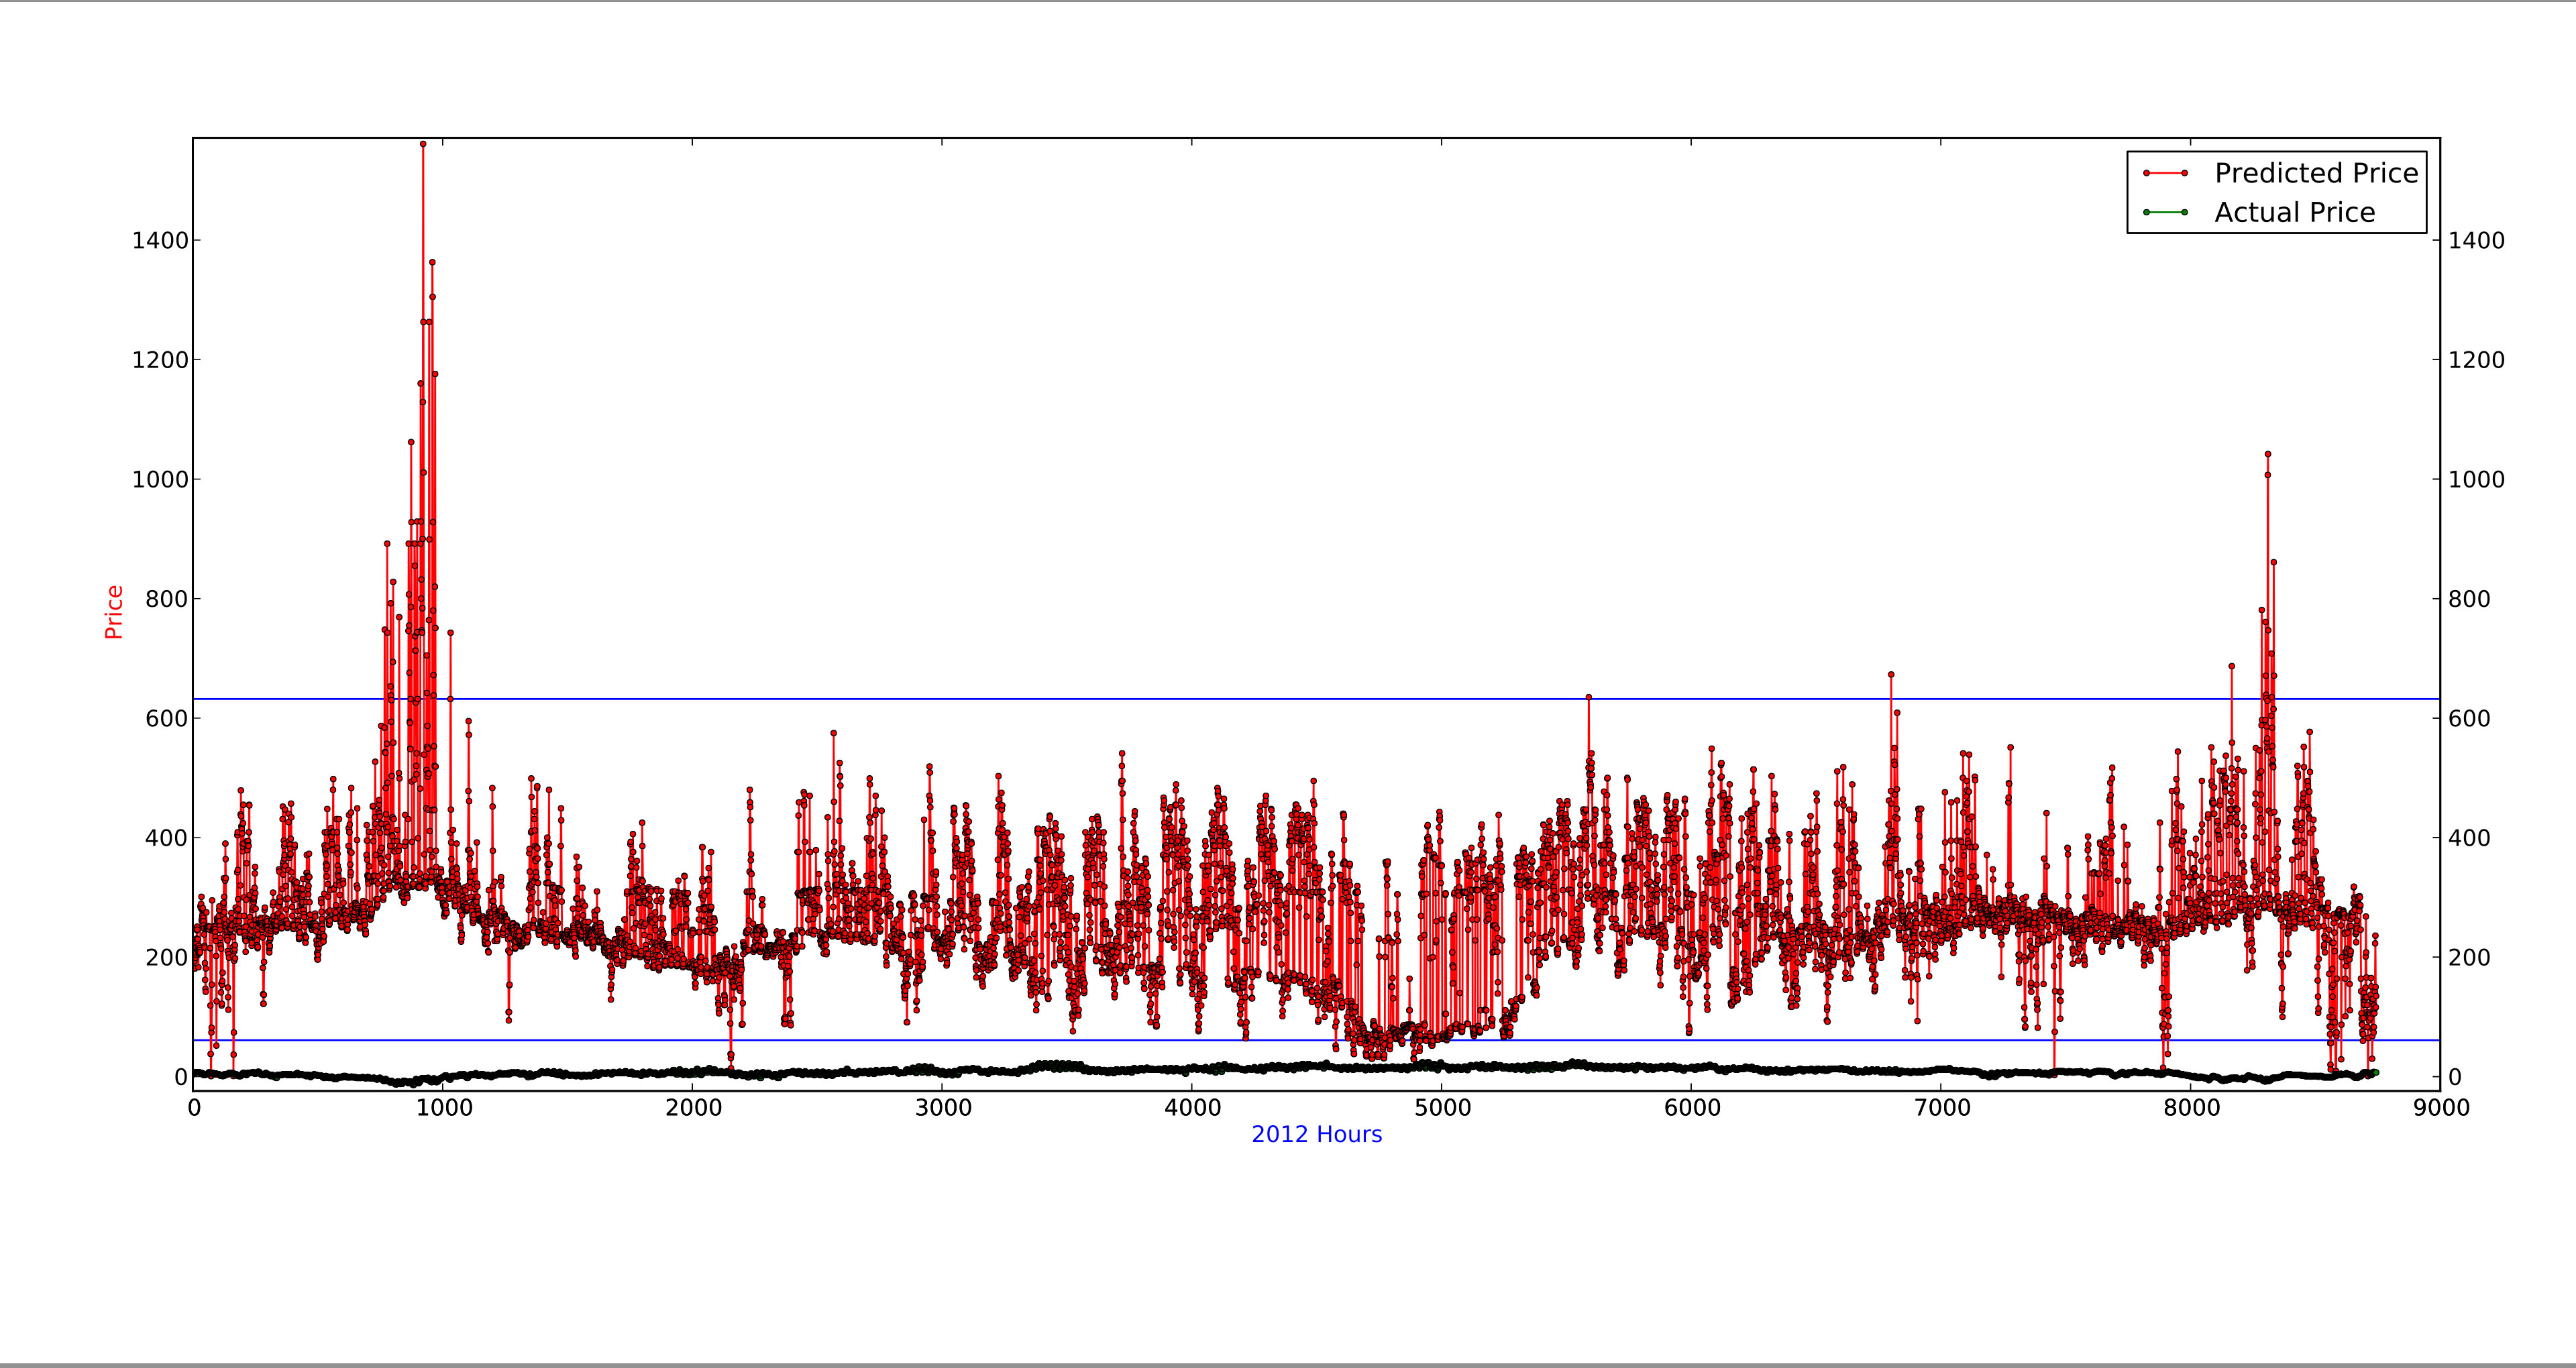
\includegraphics[width=\linewidth,natwidth=898,natheight=587]{billeder/trimming_graph.jpg}
\caption{This shows how trimming affects the prices of 2012. The blue lines show the upper and lower bounds of a 1\% trim.}
\label{fig:weight_of_layers}
\end{figure}



\subsubsection{Matrix}
When analysing the data it is possible to find a connection between different rows of data eg. what time of the day or what day of the week it is. These kind of data can be described using a single node where you normalize the hours by distributing them between -1 and 1. This will give this single neuron one weight to represent ALL of the hours in a day. One approach to give inputs more importance are splitting them up into a simple matrix. This means that we have a matrix with one row and 24 inputs(one for each hour); we set a 1 in the input representing the time of day and set the rest to 0. This way the neural network will have a specific weight to apply according to which hour of the day it is. This of course adds alot of overhead in terms of how many input nodes you need to have and how many nodes you need in the hidden layers. This will increase the processing time of the neural network iterations. This method is not only applicable with days. It can be applied to most inputs where you have a fixed and rather small set of different inputs to a single node.

\subsubsection{Historical Data}
\label{sec:historicalData}
It is the intention to achieve day-ahead forecasting by predicting the next 24 hours based on the past captured by the ANN as a generalization function  --- this can be defined as multiple step-ahead forecasting using an ANN\cite[Chapter~7.1.6]{econometrics}. 
If the analysis of a time series can identify trending behaviour then it will be of utmost importance for the forecast. The trends can be deterministic or stochastic but our time-series show stochastic properties since it at some time intervals will have a sequence of values that can lead to local trendlike movements\cite[Chapter~7.3]{econometrics}. Furthermore, it is necessary to investigate how to include this input information about the immediate past hours in order to give a better idea of what will come next. This will apply for the electricity prices but also to some extend the wind production since it follows consumption\todo{page}. It points us in the direction of simple curve analysis or statistics used in economy to capture trends of the immediate past and use it as input. The concrete methods will be discussed in more detail in sections to come. The purpose of using curve analysis would be to calculate the slope and use this as an indicator for the current trend - are we moving up or down?. This can be made more sophisticated by using actual statistics for gathering some of the price characteristics (Presented at~\ref{sec:electriciyPrices}) like frequency, seasonality and volatility. It could also be an option to include past prices as input parameters to include the historical perspective as presented in \cite{singhal2011electricity}.
What is evident is the need for analysing the price and wind production curves both to capture the tendencies but at the same time locating irregularities --- prices or productions that are so obscure that we won't be able to predict them. Experiments with the different approaches will be conducted.

\subsection{Strategies for Prediction}
\todo{present some of the strategies that we have towards prediction - maybe a summary of the above things?}
\subsubsection{Standard Inputs}

\subsubsection{Using Statistical Inputs}
\label{sec:usingStatisticalInput}
As described in the ANN section \todo{find method to point to page} in Figure~\ref{fig:overfitting} the Neural Network strives for a generalized function without overfitting so that it also applies for data outside of the trained set. In order to achieve such a function it is necessary to include enough input parameters to get a close enough fit. Every input parameter should narrow down the number of possible output values or else it makes no sense to include them. What can become problematic is when the input parameters simply result in too many output values, e.g. if similar wind speeds, air densities and temperatures would correspond to wind productions between 800-1300 \todo{concrete example from data set}. The generalization would move towards the majority of the wind productions in this interval but because the purpose of prediction is to come as close as possible to the ideal value this is not enough when the interval is too big. One way to solve this is to include a "snapshot" of the current situation as one or more input parameters so that it takes into account market trends at that time. As discussed in Historical Data~\ref{sec:historicalData} the market has certain trends \todo{ref} and if the prediction was to know the price from one hour ago and the current market trend in general it would have a better chance of guessing within the given interval. If putting this into context of the wind production interval 800-1300 --- if the last hour wind production was 1100 and the current trend is rising then the algorithm should with high probability not guess around 800 even if the majority of the wind productions is placed here. The concept is illustrated in Figure~\ref{fig:WP}\todo{make drawing}. By including the current trend as input the ANN could better approach the target to predict because it would result in a generalization of all trends in the dataset --- it would calculate how current trend in general influences the output over the entire dataset. If the majority of the rising trends in the dataset has a relatively small slope then the network would predict according to that. This will cause a problem when facing a steep slope because the ANN would not predict high enough. A solution could be to combine the statistical approach with curve analysis where the slope of the last prices and productions are taken into consideration as well. The slope says something about how much the curve is rising whereas the statistics will reflect the general trend over time. What makes it crucial is the wish to potentially predict the cases that are not general and irregular if it is possible.

Other problems arise together with the inclusion of tendency --- when have we moved enough in one direction? We need to rely on the other input parameters to pull us either up or down so that we can identify the next trend. This can possibly result in the prediction to significantly over-shoot or under-shoot its target. The statistical approach could potentially help out even more since it gives us the tool to calculate probability of the movement to come, e.g. what is the probability of the curve continuously moving up after 24. It will need to be tested thoroughly during our experiments. 

One thing to keep in mind here is that this is only a minority of the input parameters. Without these the Artificial Neural Network would have made one generalization and the addition would in theory only help the function to approach the target better when a lot of output possibilities exist. The result will be a new function where the immediate past is considered at every hour and the possibility of a improved generalization.

\begin{figure}[H]
\centering
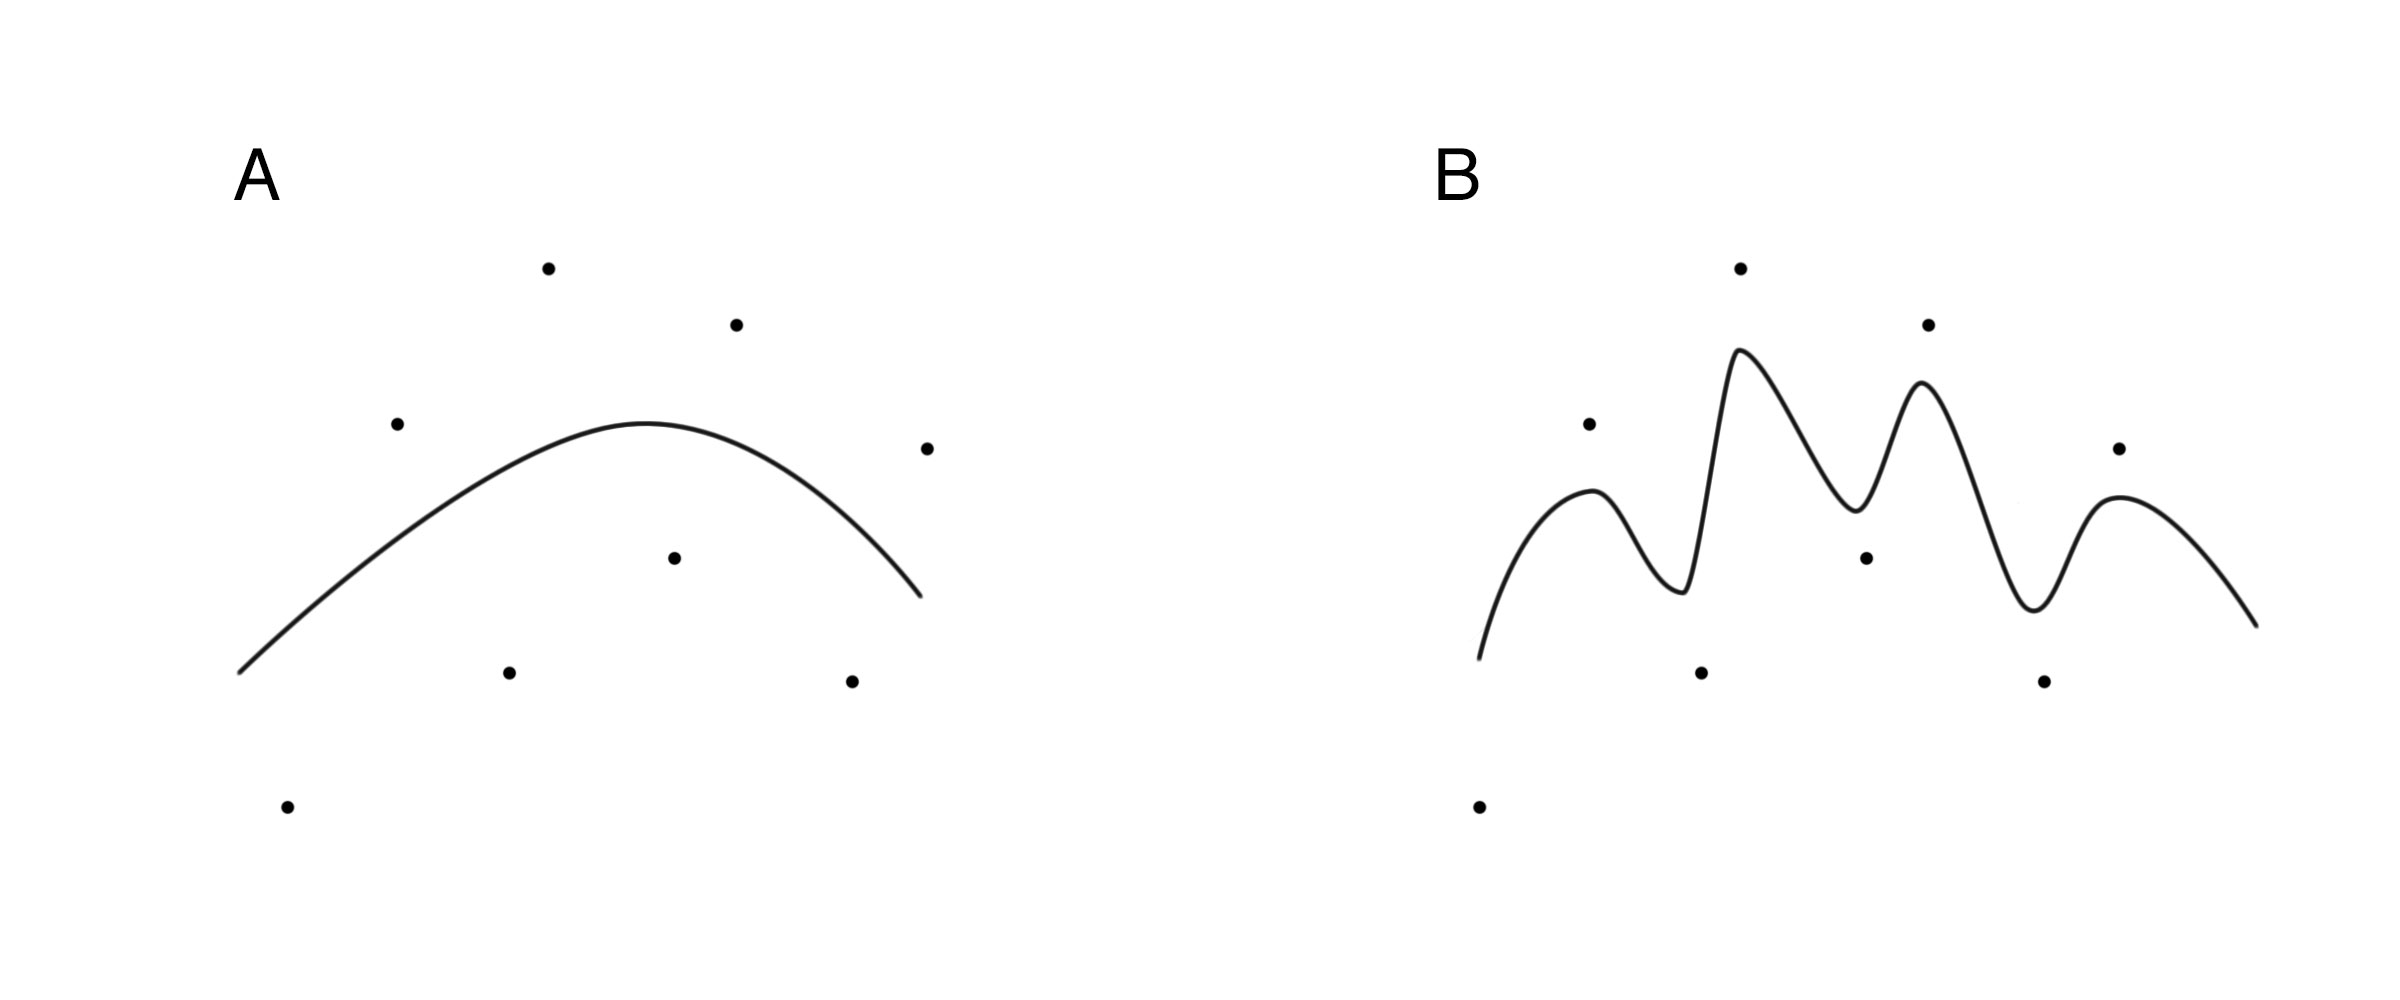
\includegraphics[width=0.99\linewidth,natwidth=898,natheight=587]{billeder/WP_000057.jpg}
\caption{A) Shows the generalized function. B) The approaching of output values}
\label{fig:WP}
\end{figure}

We will work with several statistical methods as input and with combinations of them all. 

\subsubsection{Statistical Input}
\todo{Talk about statistical input features like historical volatility (EWMA), skewness and basic calculation of line slope. Skewness is a more sophisticated way of calculating if the distribution is leaning to one sine of the mean - the simple line slope calculation is meant to calculate if we are on the way up or down}

EWMA should be used for time series that do not have a clear trend direction\cite[Chapter~7.3.2]{econometrics} which is exactly what we have. \todo{see page 588 in econometrics book}

The EWMA is a latent trend model where a latent variable is included to describe a discrete choice model. The latent variable is called the smoothing factor and if this factor is close to one then the last trend has a higher weight than the recent observation- in our case the observation would be either production or price and the smoothing factor is calculated based on the last calculated trend.

Choice of smoothing factor.

It has been used as an example for Industrial Production. 

TEGNING MULTIPE STEP

TALK ABOUT MULTIPLE-STEP-AHEAD FORECASTING --> see karlbranting

\section{Conclusion}
When modeling the ANN it is necessary to experiment with different types of inputs, hidden layers and neurons to find the best combinations. Furthermore, it is important to investigate the number of training epochs in order to find the best fit so that the ANNs training will not be under-fitted or over-fitted. We also have to experiment with the best data manipulation to find the best representation for the input parameters. When doing multiple step-ahead forecasting the immediate trend must be transferred as input to the next step, e.g. by including statistical economical features.

%%%%%%%%%%%%%%%%%%%%%%%%%%%%%%%

\chapter{Experimental Results}
\label{ch:experimentalResults}
\section{Test Procedure}
\label{sec:testProcedure}
The following high level test procedure describes the test process and environment for the experiments of both wind production and electricity prices. 
\\[0.5cm]
The construction of the neural network topology is done by incremental pruning as described in Section~\ref{sec:pruning}. The tool helps to decide the structure of the hidden layers and neurons in the network based on the pre-defined number of inputs and the output. The returned configuration is considered to the optimal structuring. Every time the input combination change pruning will be applied to discover the best possible configuration. All predictions will be based on a simulation over an entire year where 8000 hours is predicted 24 hours at a time. It is important to emphasize that the experiments are done in such a way to simulate a real-life use --- this is importance because we want the results to realistically reflect practical use. In the following experiments we consider this number of hours to be satisfying. For testing purposes and simplicity the top-3 of a experiment will be used as basis for the next. 

A more accurate prediction will always be preferred but trade-offs will be discussed and analysed. The starting number of epochs and size of dataset has been selected through simple trial and error but will be tested more thoroughly as testing progress to validate it. It is not possible or realistic to show all prediction graphs in full extend and therefore all experiments will point out only parts of the prediction graphs to highlight explanatory situations or problems relevant to the discussion or analysis at hand.     

\todo{we prune once due to time but}

We are using two datasets when predicting with the Artificial Neural Network. The training set is what the network is trained with. The testing set is unseen data that NOT contained in the training set that the network must be able to predict. The need for generalize beyond the training set is described in Section~\ref{sec:machineLearning} and makes perfect sense in a prediction context. As described Section~\ref{sec:dataCollection} that our testing set does not contain weather forecasts but actual values from 2012 but also that 24 hours weather forecasts showed an accuracy of 97\% in 2012. It must of course be taken into consideration when discussing our results.
\\[0.5cm]
The procedure for every experiment:
\begin{itemize}
\item Describe purpose.
\item Describe the expected outcome (Hypothesis).
\item Find variables to be used.
\item For all predictions in the experiment do:.
\begin{itemize}
	\item Prune network based on input parameters.
	\item Simulate the prediction of 8000 hours 24 hours at a time.
	\item Show results.
	\item Analyse results.
	\item Point out indicative parts of the prediction graphs.
\end{itemize}
\item Conclusion

\end{itemize}
\section{Statistical Evaluation Methods}
\label{sec:statisticalEvaluation}
This section described the statistical measures that will be used to determine accuracy of the predictions so that the outputs can be evaluated.

\subsubsection{MPE - Mean Percentage Error}
The Mean Percentage Erorr is the mean of the percentage-wise error when comparing the predicted value to the actual value. This value gives us the error in percent relative to the actual value. This is a standard value that a lot of people understand by just looking at it and it gives a nice indication of how big the mean error over the whole set of predictions is. The problem with this value is that it is relative to the actual value so the same error seen as a number (e.g. 20kr) will give a big difference if it is close to the minimum values predicted and a small value if it is close to the maximum values predicted; but in both cases the guess with an erorr of 20 kr is equally good. As a mathematical example:

Actual value = 1200; Predicted value = 1180; Difference = 20; Error = (20/1200)*100 = 1.67\% 

Actual value = 60; Predicted value = 80; Difference = 20; Error = (20/60) = 33.33\%

If we were to just look at the values they are fine; but when we have to compare them to how good a guess it was they are both equally good. This is a problem with the Mean Percentage Error (that the reader needs to bear in mind when reading) but it is included because of how easy it is to grasp for most people.
It is calculated by the following:
$ \frac{100\%}{n}\sum_{i=1}^{n}\frac{p_i - a_i}{a_i} $
Where $p_i$ is the predicted value and $a_i$ is the actual value.
\todo{Skal formateres ordentligt}
%\subsubsection{RMSE - Root Mean Squared Error}
\subsubsection{MAE - Mean Absolute Error}
\label{sec:maeStatistics}
The Mean Absolute Error denotes the mean of the differences between the predicted values and the actual values. This gives us an indication of how much the algorithm on average misses the target price as a value and not percent. This value is relative to the dataset and if you increase all your numbers with a factor of 10 so will the MAE thus making it very hard to compare to MAEs for other systems. The good thing about the MAE is that it is not a percentage and thus it will not get bigger if the values we predict are low (See MPE - Mean Percentage Error). That way we eliminate the problem with low values giving bigger error margins than high values even when they miss the target by the same value. It is calculated by:

 $ \frac{1}{n}\sum_{i=1}^{n}|p_i-a_i| $

 Where $p_i$ if the predicted value and $a_i$ is the actual value.

\subsubsection{MAPE - Mean Absolute Percentage Error}
The mean absolute percentage error denotes the difference between the predicted value ($p_i$) and the actual value ($a_i$) which are divided by the median($\tilde{a}$) over the whole dataset. Giving us the following formula:

\begin{align*}
\frac{1}{n}\sum_{i=1}^{n}\frac{|p_i-a_i|}{\tilde{a}}
\end{align*}

\subsubsection{PEARSONS} \label{sec:Pearsons}


STATISTIKKER
	Data Cleaning:
		Pearsons
		Trimming
		Percentile trimming

	Error evaluation:
		Mean Average Error
		Mean Squared Error
		Root 

\section{Wind Production Experiments}
\label{sec:windProductionExperiments}
This section describes the experiments that uncover the best combination of inputs and epochs as well as the different strategies. Based on the analysis of wind power from Section~\ref{sec:windPowerAnalysis} the network will try to uncover the best approach to predicting the wind power. Furthermore, experiments are needed to investigate the influence of data manipulation and statistical inputs as presented in Section~\ref{sec:usingStatisticalInput}. Additional test results and graphs can be seen in Appendix~\ref{sec:windResultsAppendix} - relevant results will be shown here. The purpose is to approach the wind power target by attempting different strategies throughout every experiment. Each experiment will either validate or reject its hypotheses and identify what influence wind power in Western Denmark (DK-1). We expect to see an improvement throughout the experiments. Figure~\ref{fig:WindPowerNetworkModel} shows a simplification of the wind power prediction model. The test procedure present the initial number of epochs as 200 and the training set size as three months --- it is based on simple trial and error.  

\begin{figure}[H]
\centering
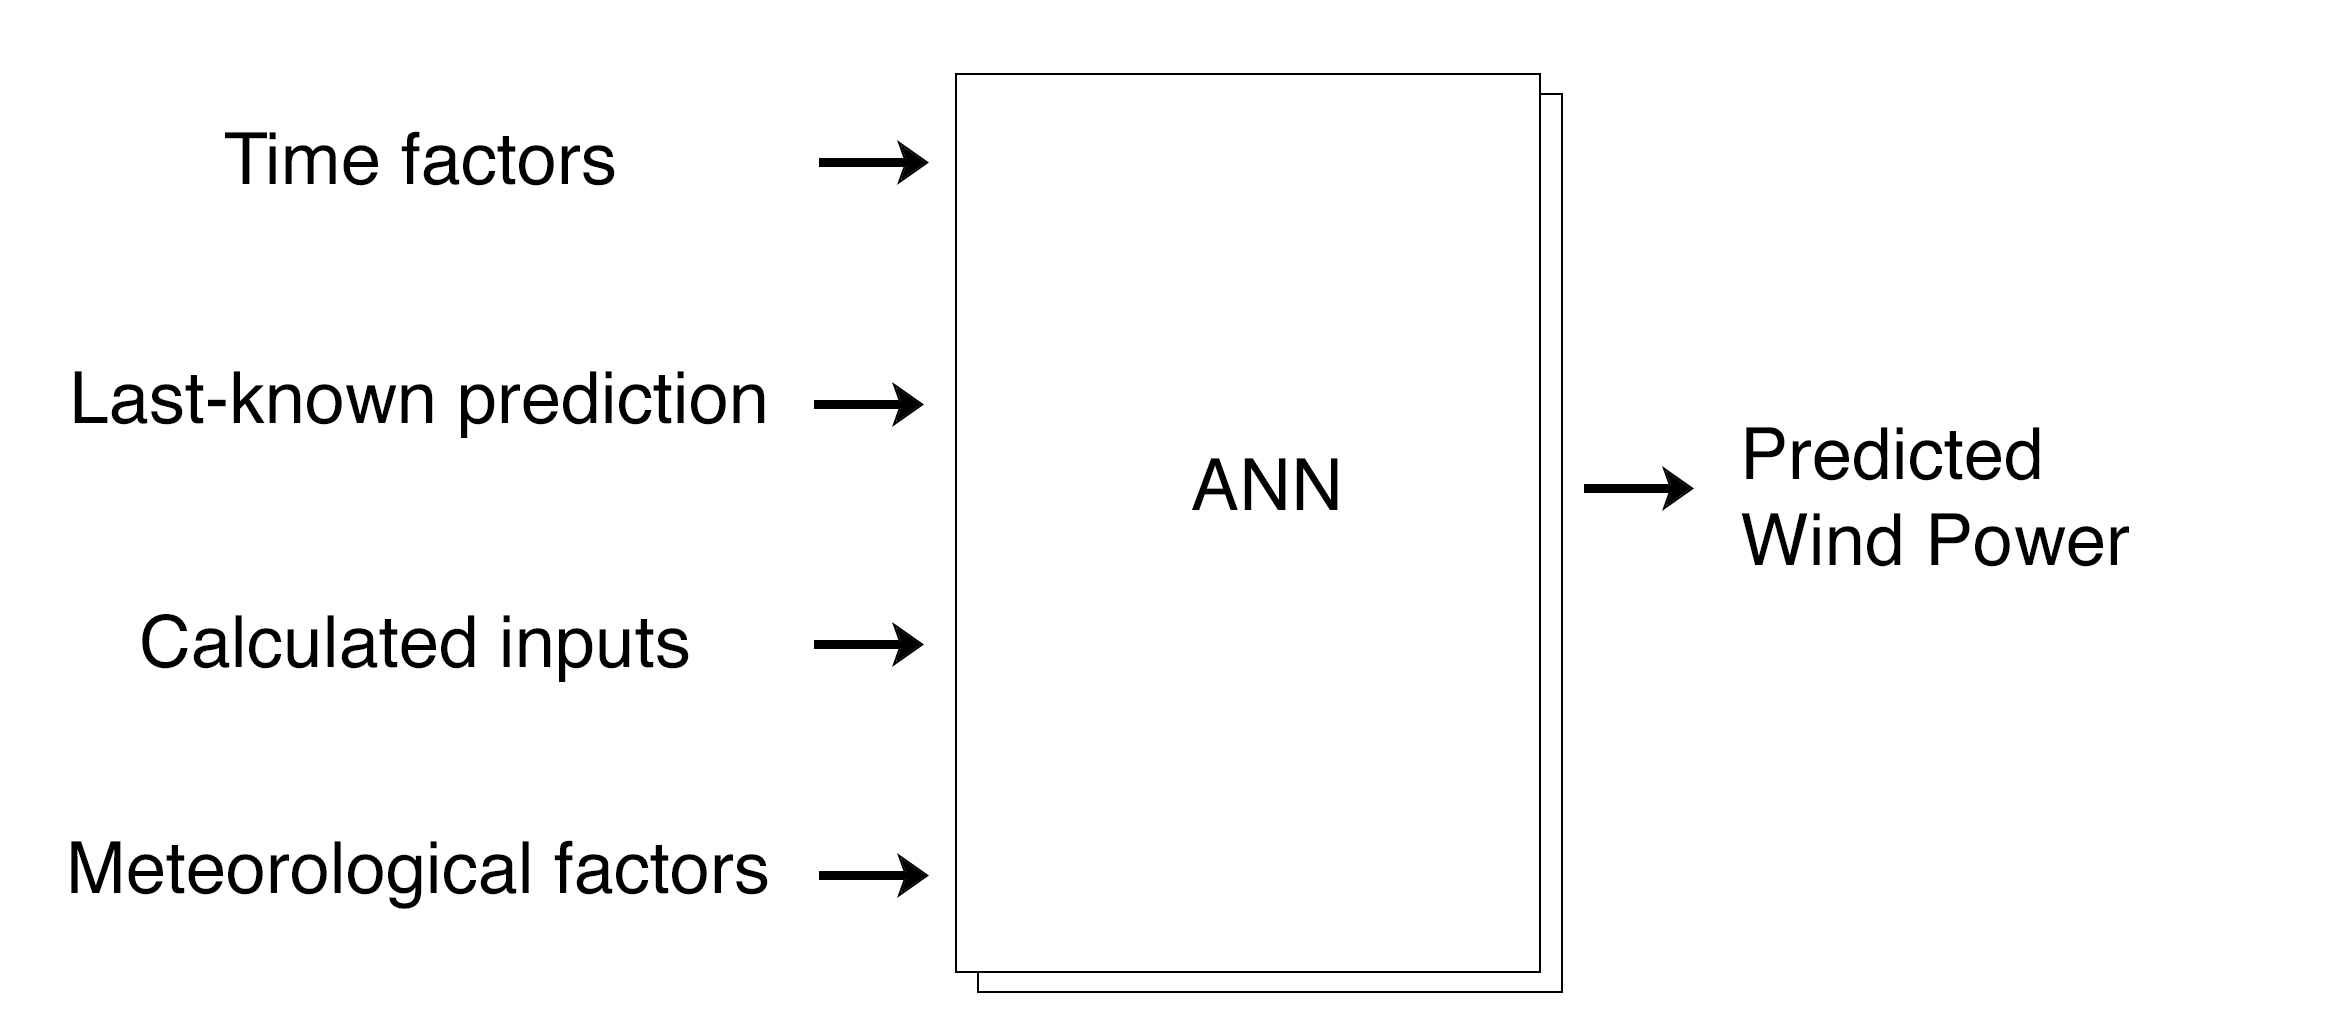
\includegraphics[width=0.99\textwidth]{billeder/WindPowerNetworkModel.png}
\caption{Simple drawing of the Feedforward Neural Network model}
\label{fig:WindPowerNetworkModel}
\end{figure} 

\subsection{Experiment One - Selection of Input Parameters}
\label{sec:windPowerExperimentOne}
The first experiment is an attempt to find the best constitution of network input parameters based on the analysis in Section~\ref{sec:windPowerAnalysis}. Since the correlation between wind power and wind speed is significant it will be included as a core input parameter in all test combinations.

\subsubsection{Hypothesis}
The analysis in Section~\ref{sec:windPowerAnalysis} uncovered the correlation between the different parameters and the wind power. The following is expected based on the analysis:

\begin{enumerate}
\item Wind speed and last known wind power are expected to be the most influential factors due to their obvious correlations to wind power. Demand showed a correlation of 0,61 and is thereby expected to influence the wind power significantly. Temperature is expected to have the potential to substitute demand but without achieving as good accuracy. 
\item Air density, time of day and month of year is expected to be of some influence. Air density is a factor in the actual formula for wind power. Time of day is connected to the demand and how it influences the wind power during the day. Month of year is relation seasonality and the weather changes during the year that will affect the wind power. 
\item Wind direction is expected to be of some influence based on how it is used in the area of windmill placement as presented in Section~\ref{sec:windmillPlacement}.
\end{enumerate}

\subsubsection{Variables}
The variables used in this experiment series:

\begin{itemize}
\item Wind speed (WS)
\item Air density (AD)
\item Demand (D)
\item Time of day (ToD)
\item Temperature (T)
\item Wind direction (WD)
\item Last known production (L-P)
\item Month (Mo)
\end{itemize}

The different tables contain following abbreviations:

\begin{itemize}
\item How many percentage of the predictions in the correct direction (\% CD)
\item Neurons in hidden layer 1 (H1)
\item Neurons in hidden layer 2 (H2)
\item Percentage rank from the best prediction (\% Rank)
\end{itemize}

\subsubsection{Results}
\label{sec:predictionBasicInputParams}
Experiments have been conducted for all possible input combinations. The idea is to discover any unforeseen connections found by the Feedforward Neural Network. The results can be found in Appendix~\ref{sec:simpleInputTest} but relevant results will be emphasized here. The results vary in MAE from 127,86 to 199,22. Table~\ref{table:windProdInputParamsTop10} highlight the top and bottom 10 for further analysis. One thing that is not observable from the table is the use of wind speed as the only input for prediction which achieves 149,72 in MAE over the entire year which illustrate the expected relationship between wind speed and wind power. The \% CD in the table is an indication of how many predicted hours was in correct direction compared to the actual direction. The percentage is stable throughout the table with values around 60-70\%. The correct direction percentage is around the same for the bottom 10. It indicates what have been discussed before, namely wind power follows the trends of the wind speed and it is included in all of the predictions. This will be discussed further when looking at the actual prediction graph.

\footnotesize
\begin{center}
\begin{longtable}{|c|c|c|c|c|c|c|c|c|c|c|c|c|}
\hline
\textbf{WS} & \textbf{AD} & \textbf{D} & \textbf{T} & \textbf{WD} & \textbf{L-P} & \textbf{Mo}& \textbf{ToD} & \textbf{MAE} & \textbf{\% Rank} & \textbf{H1} & \textbf{H2} & \textbf{\% CD}  \\
\hline
\endfirsthead
\multicolumn{13}{c}%
{\tablename\ \thetable\ -- \textit{Continued from previous page}} \\
\hline
\textbf{WS} & \textbf{AD} & \textbf{D} & \textbf{T} & \textbf{WD} & \textbf{L-P} & \textbf{Mo}& \textbf{ToD} & \textbf{MAE} & \textbf{\% Rank} & \textbf{H1} & \textbf{H2} & \textbf{\% CD} \\
\hline
\endhead
\hline \multicolumn{13}{r}{\textit{Continued on next page}} \\
\endfoot
\endlastfoot
\arrayrulecolor{light-gray}
 \x &  &  &  \x &  &  \x &  &  \x & 128,32 & 0,0\% & 24 & 1 & 73\% \\ \hline
 \x &  \x &  &  &  \x &  \x &  &  \x & 131,59 & 2,55\% & 17 & 1 & 73\% \\ \hline
 \x &  \x &  &  &  &  \x &  &  \x & 131,89 & 2,78\% & 12 & 1 & 73\% \\ \hline
 \x &  \x &  \x &  \x &  \x &  \x &  &  \x & 133,18 & 3,79\% & 22 & 1 & 72\% \\ \hline
 \x &  \x &  \x &  \x &  \x &  \x &  &  & 133,77 & 4,25\% & 24 & 1 & 73\% \\ \hline
 \x &  \x &  \x &  &  &  \x &  &  \x & 134,14 & 4,54\% & 19 & 1 & 73\% \\ \hline
 \x &  \x &  \x &  &  \x &  \x &  &  \x & 135,4 & 5,52\% & 25 & 1 & 72\% \\ \hline
 \x &  \x &  \x &  &  &  \x &  &  & 136,33 & 6,24\% & 15 & 1 & 73\% \\ \hline
 \x &  \x &  &  &  &  \x &  \x &  \x & 136,65 & 6,49\% & 11 & 1 & 73\% \\ \hline
 \x &  &  &  &  &  \x &  &  & 137,33 & 7,02\% & 1 & 0 & 74\% \\ \hline
 . & . & . & . &  .  & . &  . & . & . & . & . & . & . \\ \hline
 . & . & . & . &  .  & . &  . & . & . & . & . & . & .\\ \hline
 . & . & . & . &  .  & . &  . & . & . & .& . & . & .\\ \hline
 \x &  \x &  &  \x &  &  \x &  \x &  & 170,93 & 33,21\% & 21 & 1 & 71\% \\ \hline
 \x &  &  \x &  \x &  \x &  \x &  \x &  \x & 171,61 & 33,74\% & 23 & 1 & 71\% \\ \hline
 \x &  &  \x &  \x &  &  \x &  \x &  & 172,72 & 34,6\% & 21 & 1 & 71\% \\ \hline
 \x &  &  &  &  \x &  \x &  \x &  & 173,12 & 34,91\% & 17 & 1 & 71\% \\ \hline
 \x &  &  \x &  \x &  &  \x &  \x &  \x & 173,65 & 35,33\% & 12 & 1 & 69\% \\ \hline
 \x &  \x &  \x &  \x &  \x &  \x &  \x &  \x & 174,26 & 35,8\% & 17 & 1 & 68\% \\ \hline
 \x &  \x &  &  \x &  &  \x &  \x &  \x & 174,55 & 36,03\% & 21 & 1 & 71\% \\ \hline
 \x &  &  &  \x &  &  \x &  \x &  \x & 174,85 & 36,26\% & 18 & 1 & 70\% \\ \hline
 \x &  \x &  \x &  &  \x &  \x &  \x &  & 180,89 & 40,97\% & 14 & 1 & 68\% \\ \hline
 \x &  \x &  &  &  \x &  \x &  \x &  \x & 199,22 & 55,25\% & 22 & 1 & 70\% \\ \hline
\caption{Wind power Input Parameter Test Top and bottom 10. It is based on 3 month of historical data and 200 epochs. It is an average of the prediction over 8000 hours}
\label{table:windProdInputParamsTop10}
\end{longtable}
\end{center}
\normalsize

\subsubsection{Meteorological Factors}
The contents of the Table~\ref{table:windProdInputParamsTop10} indicates that air density is significant. It corresponds well with the analysis in Section~\ref{sec:windPowerAnalysis} where the relationship between wind power and these air density established to be of significance. Furthermore, it is established in Section~\ref{sec:windmillPlacement} that air density is included in the actual formula for calculating wind power.

Wind Direction is represented four times in top 10. What is noticeable is the same combinations without wind direction is also represented. This can suggest the indifference of wind direction, e.g. \#2-\#3 and \#6-\#7 is very similar. This is further backed up by the analysis which only showed a low correlation.

\subsubsection{Demand}
Demand is only represented five times in top 10 which comes as a surprise due to the correlation of 0,61 established in the analysis of wind power. The demand showed a close relationship with temperature and the explanation can be a substitution of the two. Air density represents temperature since it is the significant factor in its calculation due to the pressure being close to constant in the dataset as described in Section~\ref{sec:airDensity}. This is the most plausible explanation of the top-3 being without demand.

\subsection{Last Known Wind Power}
Last known wind power is as expected represented in all of top 10 according to the analysis of wind power development in Section~\ref{sec:windProductionDev}. It complies well with the how previous hours was established to have an impact on the movements of the curve. All of the bottom 10 also contains last known wind power but the reason can be found in the inclusion of month. The worst prediction just without month is placed as number three --- the explanation can reside in the size of the training set but this will be discussed later. The inclusion of previous hours will be attempted more sophistically in the experiment about calculated inputs but.

\subsubsection{Seasonality as Month}
Month was expected to have an influence on wind power since the the difference between wind power during summer and winter months showed to be significant (from 500 in average during August to above an average of 1000 during December and January). Therefore it comes as a surprise that the contributory cause to the bad accuracy in the bottom is month. It does in general not help the prediction when used together with a dataset containing only three months. Month represents the seasonal perspective of the input parameters and is suppose to find the relationship between months and the wind power in general. Since the historical data used for prediction is only three months, it does not capture how the same month last year influenced the production. In the case of wind power prediction it seems to be creating more noise and thereby affect the prediction badly. A possible solution to obtain the seasonality aspect is presented in\cite{pjmForecast} where the Neural Network is trained with 45 days from before the day to be predicted, and 45 days before and after it in the previous year. By using this approach the month parameter will reflect the influence of the months around you from the last year. This will be validated in a prediction later in experiment one.

\subsubsection{Importance of testing set}
We describe in our testing procedure that we use a separate training set and a testing set. Table~\ref{table:predictionMAEUnseenVsTrainingSet} emphasize the importance of using a testing set containing only unseen data. The purpose is to generalize beyond the data in the training set and give accurate outputs for unseen data \cite{1} --- the prediction must simulate real use where the training set naturally cannot contain known data. It is also noticeable that the MAE is similar from top to bottom. We will only consider the MAE coming from predictions of the testing set.

\footnotesize
\begin{center}
\begin{longtable}{|c|c|c|c|}
\hline
\textbf{MAPE (test set)} & \textbf{MAE (test set)} & \textbf{MAE (training set)} & \textbf{MAPE (training set)}  \\
\hline
\endfirsthead
\multicolumn{4}{c}%
{\tablename\ \thetable\ -- \textit{Continued from previous page}} \\
\hline
\textbf{MAPE (test set)} & \textbf{MAE (test set)} & \textbf{MAE (training set)} & \textbf{MAPE (training set)}  \\
\hline
\endhead
\hline \multicolumn{4}{r}{\textit{Continued on next page}} \\
\endfoot
\endlastfoot
\arrayrulecolor{light-gray}
19,34\% & 128,32 & 60,02 & 9,05\%  \\ \hline
19,74\% & 131,59 & 51,54 & 7,73\%  \\ \hline
19,79\% & 131,89 & 51,73 & 7,76\%  \\ \hline
19,98\% & 133,18 & 60,29 & 9,05\%  \\ \hline
20,07\% & 133,77 & 52,17 & 7,83\%  \\ \hline
20,13\% & 134,14 & 54,79 & 8,22\%  \\ \hline
20,32\% & 135,4 & 50,57 & 7,59\%  \\ \hline
20,45\% & 136,33 & 51,69 & 7,76\%  \\ \hline
20,5\% & 136,65 & 53,99 & 8,1\%  \\ \hline
19,76\% & 137,33 & 58,55 & 8,42\%  \\ \hline
 . & . &  . & . \\ \hline 
 . & . &  . & . \\ \hline 
 . & . &  . & . \\ \hline
25,65\% & 170,93 & 51,67 & 7,75\%  \\ \hline
25,75\% & 171,61 & 50,58 & 7,59\%  \\ \hline
25,91\% & 172,72 & 54,5 & 8,18\%  \\ \hline
25,97\% & 173,12 & 53,15 & 7,97\%  \\ \hline
26,05\% & 173,65 & 51,82 & 7,77\%  \\ \hline
26,15\% & 174,26 & 49,84 & 7,48\%  \\ \hline
26,19\% & 174,55 & 54,28 & 8,14\%  \\ \hline
26,23\% & 174,85 & 49,75 & 7,46\%  \\ \hline
27,14\% & 180,89 & 50,92 & 7,64\%  \\ \hline
29,89\% & 199,22 & 52,03 & 7,81\%  \\ \hline
\caption{Average prediction MAE/MAPE on unseen data vs. prediction MAE/MAPE on training set}
\label{table:predictionMAEUnseenVsTrainingSet}
\end{longtable}
\end{center}
\normalsize

\subsubsection{Seasonal aspect}
\label{sec:predictionWindProdSeasonalExperiment}
The discussion above revealed the need for uncovering and discussing how to represent the seasonal aspect (if needed at all) in Feedforward Neural Network --- it can be included as a explicit input parameter or implicitly in the dataset by using the right training set size. The training set will be explored with two different sizes in an attempt to express the seasonal aspect with month as input:

\begin{enumerate}
\item Basing it on \cite{pjmForecast} where the training set is constructed with 45 days from before the day to be predicted, 45 days before and after in the previous year. Here called 135 Days Approach.
\item Using a year before the day to predict. We reference to it as Whole Year Approach.
\end{enumerate}

\subsubsection{135 Days Approach}
The experimental results for (1) are all shown in Appendix~\ref{sec:simpleInputTestSeason} but we will only be focusing on top-10 here because they illustrate the problem. The results are decreased in all of the predictions in Table~\ref{table:seasonalWindProdInputParamsTop10} in comparison with the the results training on 3 months of data. The training set is increased and this might make it harder for the ANN to generalize because too large training sets should according to \cite{1} be avoided due to a tendency to over-train. It can be supported by the similar results only differentiated by 1,12\% from \#1-\#10 --- the network generalizes on much more data and if some values only influence the wind power in smaller periods of the year it will be suffocated between the ones that are important (as with the importance of wind speed) over the entire year. The network can over-train itself by dedicating to much responsibility to wind speed because it in general is the most important input or the dataset can simply contain too much noise. The possible benefits from including the seasonal aspect when predicting wind power is not enough to make up for the loss in accuracy by the increase of training set size, e.g. month is only included once in top-10. Before any final conclusions about the size of training set can be made we will have to conduct the experiment on an entire year.

\footnotesize
\begin{center}
\begin{longtable}{|c|c|c|c|c|c|c|c|c|c|c|c|c|}
\hline
\textbf{WS} & \textbf{AD} & \textbf{D} & \textbf{T} & \textbf{WD} & \textbf{L-P} & \textbf{Mo}& \textbf{ToD} & \textbf{MAE} & \textbf{\% Rank} & \textbf{H1} & \textbf{H2} & \textbf{\% CD} \\
\hline
\endfirsthead
\multicolumn{13}{c}%
{\tablename\ \thetable\ -- \textit{Continued from previous page}} \\
\hline
\textbf{WS} & \textbf{AD} & \textbf{D} & \textbf{T} & \textbf{WD} & \textbf{L-P} & \textbf{Mo}& \textbf{ToD} & \textbf{MAE} & \textbf{\% Rank} & \textbf{H1} & \textbf{H2} & \textbf{\% CD} \\
\hline
\endhead
\hline \multicolumn{13}{r}{\textit{Continued on next page}} \\
\endfoot
\endlastfoot
\arrayrulecolor{light-gray}
 \x &  \x &  \x &  &  \x &  \x &  &  \x & 142,88 & 0,0\% & 7 & 17 & 73\% \\ \hline
 \x &  &  &  \x &  \x &  \x &  &  \x & 142,89 & 0,01\% & 14 & 11 & 73\% \\ \hline
 \x &  \x &  &  &  \x &  \x &  &  \x & 143,37 & 0,34\% & 3 & 21 & 73\% \\ \hline
 \x &  \x &  \x &  \x &  \x &  \x &  &  \x & 143,97 & 0,76\% & 4 & 25 & 72\% \\ \hline
 \x &  &  &  &  &  \x &  &  \x & 143,98 & 0,77\% & 2 & 21 & 72\% \\ \hline
 \x &  \x &  \x &  \x &  &  \x &  \x &  \x & 144,11 & 0,86\% & 1 & 17 & 73\% \\ \hline
 \x &  \x &  &  &  &  \x &  &  \x & 144,12 & 0,87\% & 7 & 12 & 73\% \\ \hline
 \x &  &  &  &  &  &  &  \x & 144,28 & 0,98\% & 12 & 17 & 41\% \\ \hline
 \x &  &  \x &  &  \x &  \x &  &  \x & 144,42 & 1,08\% & 11 & 10 & 72\% \\ \hline
 \x &  \x &  &  \x &  \x &  \x &  &  \x & 144,48 & 1,12\% & 1 & 17 & 73\% \\ \hline
\caption{Top 10 seasonal wind power test. It is based on 3 month of historical data and one month after from the previous year. It is run with 200 epochs and predicts 8000 hours in 2012}
\label{table:seasonalWindProdInputParamsTop10}
\end{longtable}
\end{center}
\normalsize

Table~\ref{table:predictionMAEUnseenVsTrainingSetSeasonality} is included to show MAPE and highlight what was discussed regarding the use of a testing set with unseen data.

\footnotesize
\begin{center}
\begin{longtable}{|c|c|c|c|}
\hline
\textbf{MAPE (test set)} & \textbf{MAE (test set)} & \textbf{MAE (training set)} & \textbf{MAPE (training set)}  \\
\hline
\endfirsthead
\multicolumn{4}{c}%
{\tablename\ \thetable\ -- \textit{Continued from previous page}} \\
\hline
\textbf{MAPE (test set)} & \textbf{MAE (test set)} & \textbf{MAE (training set)} & \textbf{MAPE (training set)}  \\
\hline
\endhead
\hline \multicolumn{4}{r}{\textit{Continued on next page}} \\
\endfoot
\endlastfoot
\arrayrulecolor{light-gray}
21,44\% & 142,88 & 51.17 & 7.68\% \\ \hline
21,44\% & 142,89 & 50.08 & 7.51\% \\ \hline
21,51\% & 143,37 & 52.01 & 7.8\% \\ \hline
21,6\% & 143,97 & 48.2 & 7.23\% \\ \hline
21,6\% & 143,98 & 49.51 & 7.43\% \\ \hline
21,62\% & 144,11 & 49.31 & 7.4\% \\ \hline
21,62\% & 144,12 & 49.29 & 7.4\% \\ \hline
21,65\% & 144,28 & 121.29 & 18.2\% \\ \hline
21,67\% & 144,42 & 50.5 & 7.58\% \\ \hline
21,68\% & 144,48 & 47.67 & 7.15\% \\ \hline
\caption{Average prediction MAE/MAPE on unseen data vs. prediction MAE/MAPE on training set with seasonality}
\label{table:predictionMAEUnseenVsTrainingSetSeasonality}
\end{longtable}
\end{center}
\normalsize

\subsubsection{Whole Year Approach} 
The second experiment where the prediction is based on an entire years training set can be seen in Table~\ref{table:seasonWindProdInputParamsTop2WholeYear}. The MAE is much similar to the first seasonal approach from Table~\ref{table:seasonalWindProdInputParamsTop10} but instead it takes longer time to process because it must train on a larger dataset --- the time aspect will be elaborated in another experiment. Leaving out the seasonal aspect is the obvious choice from the results shown here. Using a training set of 3 months can be argued to contain the seasonal aspect because the set will reflect how the input parameters in general influence the wind power in the current season. Including month or increasing the size of the training set will only add noise and make it harder for the ANN to generalize. The purpose of including month was to avoid problems when encountering a seasonal change due the different conditions from season to season (analysis confirms this). If the same conditions were seen last year then this could be incorporated in the generalization. The results show that the benefits from this approach cannot make up for the small dataset implicitly containing the seasonal aspect. The month parameter will be omitted in experiments to come.   			

\footnotesize
\begin{center}
\begin{longtable}{|c|c|c|c|c|c|c|c|c|c|c|c|c|}
\hline
\textbf{WS} & \textbf{AD} & \textbf{D} & \textbf{T} & \textbf{WD} & \textbf{L-P} & \textbf{Mo}& \textbf{ToD} & \textbf{MAE} & \textbf{MAPE} & \textbf{H1} & \textbf{H2} & \textbf{\% CD}  \\
\hline
\endfirsthead
\multicolumn{13}{c}%
{\tablename\ \thetable\ -- \textit{Continued from previous page}} \\
\hline
\textbf{WS} & \textbf{AD} & \textbf{D} & \textbf{T} & \textbf{WD} & \textbf{L-P} & \textbf{Mo}& \textbf{ToD} & \textbf{MAE} & \textbf{H1} & \textbf{H2} & \textbf{\% CD} \\
\hline
\endhead
\hline \multicolumn{13}{r}{\textit{Continued on next page}} \\
\endfoot
\endlastfoot
\arrayrulecolor{light-gray}
 \x &  \x &  \x &  \x &  &  \x &  \x &  & 147,98 & 22,12\% & 6 & 22 & 73\% \\ \hline
\caption{Seasonal wind power test based on an entire year. It is run with 200 epochs and predicts 8000 hours in 2012}
\label{table:seasonWindProdInputParamsTop2WholeYear}
\end{longtable}
\end{center}
\normalsize

\subsubsection{Best prediction graph}
\label{sec:bestInputCombiGraph}
The first 175 hours of the best prediction from Table~\ref{table:windProdInputParamsTop10} can be seen in Figure~\ref{fig:bestInputParameterPrediction}. The hours have been pointed out because they illustrate situations and issues that are relevant for the analysis and general for the prediction - more graphs can be seen in Appendix~\ref{sec:bestCombiPredictionsGraphs}. It can be observed that the prediction follows the trend of the actual wind power which is also emphasized by the correct direction percentage of 73\%. The graph shows how the challenge is the number of steps it takes to identify shifting trends and how much the trend is increasing or decreasing at that particular time. The green and purple overlay show situations where it is behind the actual trend whereas the yellow overlay illustrates how it is able to identify the rising trend shortly after prediction time (illustrated by the vertical lines) but too early and ends up overshooting. One last comment is in relation to the error visualization in the bottom of the graph and how it follows the curve of the actual wind power productions.  

\begin{figure}[H]
\centering
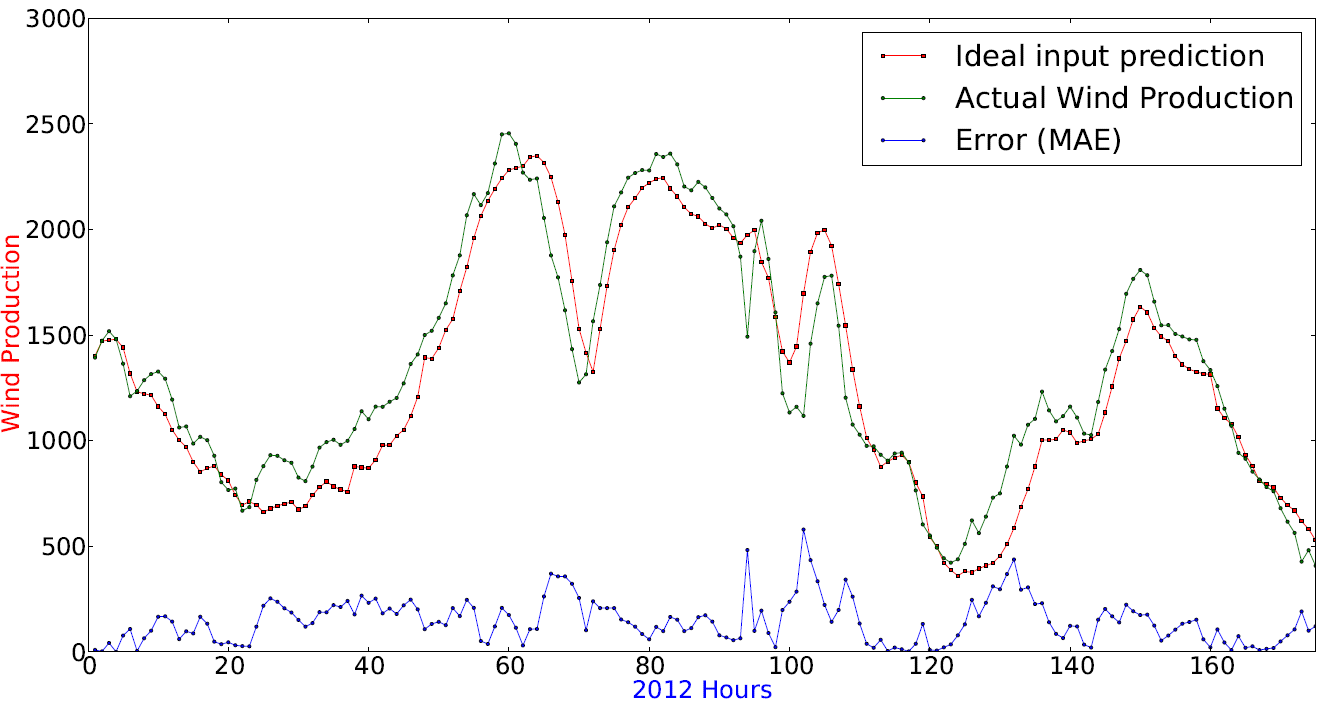
\includegraphics[width=0.99\textwidth]{billeder/bestInputParameterPrediction.png}
\caption{Wind power prediction for 0-175 hours in 2012 with the best combination}
\label{fig:bestInputParameterPrediction}
\end{figure} 

The three overlay situations are emphasized because they show a general problem. Taking a closer look at the purple overlay (hours 120-148) in Figure~\ref{fig:bestInputCombi120-148} illustrates how the prediction is accurate in the beginning but has trouble identifying the significance of the rising trend and continues to under-shoot throughout the entire 24-hours forecast. Every step is based on the prediction from the previous step which is likely to result in an elevated error until a shift in trend.

\begin{figure}[H]
\centering
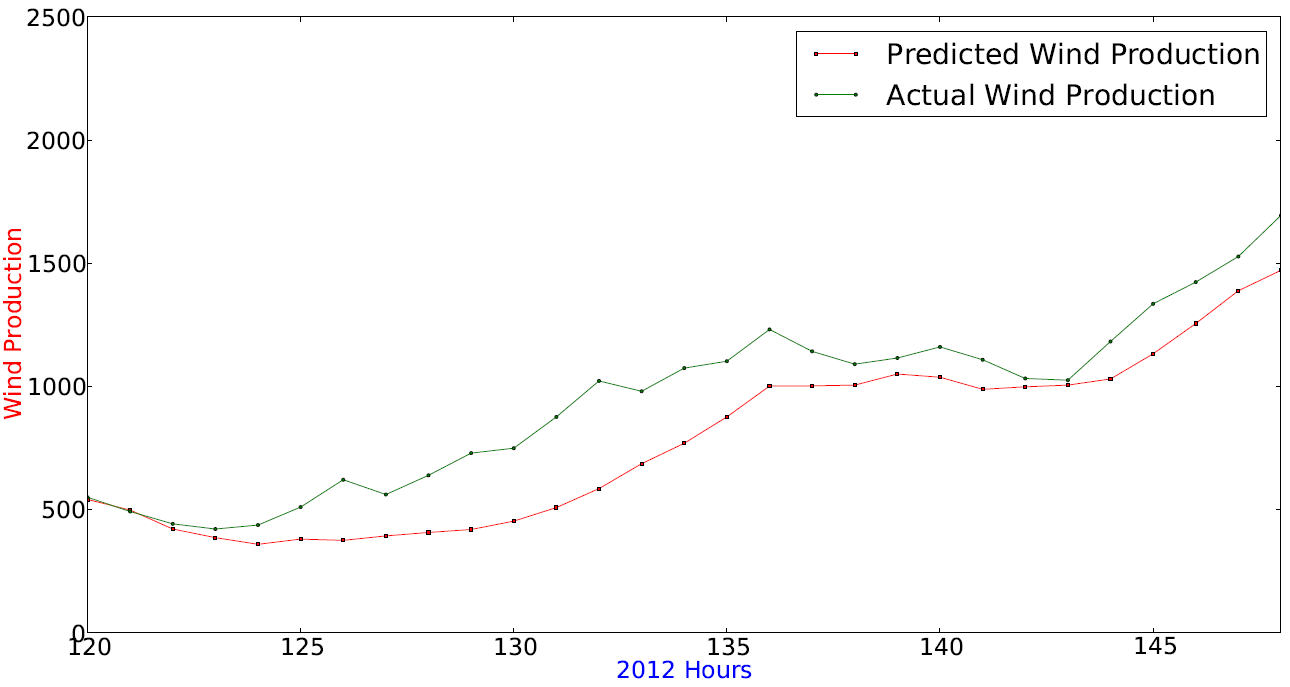
\includegraphics[width=0.99\textwidth]{billeder/bestInputCombi120-148.png}
\caption{Wind power prediction for 24 hours between 120 and 148}
\label{fig:bestInputCombi120-148}
\end{figure} 

The opposite situation where we instead see an example of overshooting in the yellow overlay (96-120) is shown in Figure~\ref{fig:bestInputCombi96-120}. It is observable how the prediction again follows accurately in the first couple of hours but then identifies the shift too early and overshoots. When the trend shifts again it is able to find its way back, e.g. the error is not elevated from start to end but only per trend. What is meant by "per trend" is if the curve is shifting direction and the prediction does not identify it at once it will elevate the error until the trend shifts again. 

\begin{figure}[H]
\centering
\includegraphics[width=0.99\textwidth]{billeder/bestInputCombi96-120.png}
\caption{Wind power prediction for 24 hours between 96 and 120}
\label{fig:bestInputCombi96-120}
\end{figure} 

What is noticeable from the examples is the problems that arise due to the 24-ahead prediction indicated by the vertical lines in Figure~\ref{fig:bestInputParameterPrediction}. Every hour is based on the previous prediction (except from the first of course) which makes it prone to error if one step fails whilst following a certain direction. It is also obvious that the error is not elevated all the way to the end but only until a new shift in trend is identified then it can correct itself. The calculated approach described in Section~\ref{sec:usingStatisticalInput} can possible help in these cases by calculating trend or slope and use it as input to add further characteristics of the curve. Later experiments will take up the calculated input approach for comparison.

The graph in Figure~\ref{fig:bestInputParameterLowNumbers} has been highlighted to show how the best prediction in general performs on low numbers and how it is able to follow the trend all the way from the bottom and up when the wind power is not as volatile (as with the other examples) within the sliding window. High volatility is seen in Figure~\ref{fig:bestInputCombi4500-4700} and again highlights (this time red) the difficulties in predicting something that is volatile within a short period of time.

\begin{figure}[H]
\centering
\includegraphics[width=0.99\textwidth]{billeder/bestInputParameterLowNumbers.png}
\caption{Wind power prediction for 5000-5175 hours in 2012 with the best combination}
\label{fig:bestInputParameterLowNumbers}
\end{figure} 

\begin{figure}[H]
\centering
\includegraphics[width=0.99\textwidth]{billeder/bestInputCombi4500-4700.png}
\caption{Wind power prediction for 4500-4700 hours in 2012 with the best combination}
\label{fig:bestInputCombi4500-4700}
\end{figure} 

The correct direction percentage for the best prediction is 73\%. When looking at the graph in Figure~\ref{fig:bestInputCombi4500-4700} some of the obvious wrong directions can be observed in the two red boxes. When the volatility of the productions are low or less significant then these trends are difficult to identify especially when numbers are smaller as seen Figure~\ref{fig:bestInputParameterLowNumbers} from hours 5000-5060.

\subsubsection{Conclusion}
All results of the first experiment can be seen in Appendix~\ref{sec:windResultsAppendix}. The best result can be seen in Table~\ref{table:windProdInputParamsTop10} and achieves a MAE of 128,32. The following conclusions can be made: 

\begin{enumerate}
\item Wind speed showed as expected to have very high significance when predicting the wind power. Demand was not represented in top-3 even though it showed very good correlation in the analysis. The good relationship between temperature and demand is described in Section~\ref{sec:demandWindProduction} which can explain why demand in top-3 is omitted and substituted with either air density or temperature. The analysis in Section~\ref{sec:airDensity} describes how air density is calculated with temperature as the most significant factor since pressure is close to constant in the dataset.   
\item Last known wind power is highly represented in both top-10 and bottom-10. It is important when put together with the right combination but whenever in combination with month of year it worsens. Month did not help the prediction even though the dataset was increased to better incorporate the seasonality aspect. Air density and time of day both showed to be highly represented in top-10 together with wind speed and last known production.
\item Wind direction was expected to have some influence but showed itself four times in top-10. It is assumed that direction is of some importance but not much based on the exact same constitution of input parameters just without wind direction achieved close to same result.
\end{enumerate}

The experiments to come will be based on input combinations from the top 3 from Table~\ref{table:windProdInputParamsTop10}. The inputs are:
\begin{itemize}
\item Wind speed;
\item Air density;
\item Wind Direction;
\item Temperature;
\item Last known production;
\item Time of day;
\end{itemize}
\newpage
\subsection{Experiment Two - Data Manipulation}
\label{sec:windProdExperimentTwo}
Experiment two tries to discover the best way to represent the input data. The need for manipulating the data can arise if irregularities exist that cannot be predicted or simply to adjust the data to better fit the inner workings of the Feedforward Neural Network. The 3 approaches to data manipulation tested in the thesis is normalization, trimming and using a matrix as input. The necessity is described in more detail in Section~\ref{sec:DataManipulation}. Normalization is necessary for all input and is used in all experiments because the sigmoid function is used as activation function. Trimming is used to trim away irregularities if such exist but it does not apply for predicting wind power (see Section~\ref{sec:windProductionDev}). It does not leave out the possibility of scenarios where trimming makes sense when used in the hand of an expert, e.g. if experience can eliminate certain high values in the next 24 hours then they could be trimmed. We will investigate whether or not trimming makes the predicted values more accurate. Tests have been conducted to show the possible benefits from using trimming on wind power. The purpose of experiment two is to turn inputs into a matrix whenever it makes sense and see the possible benefit of trimming. The matrix representation can be used as an augmentation of the best input parameters already discovered since it helps express the existing input better. As described in Section~\ref{sec:Matrix} wind speed is split into one input parameter for all of its possible values. Each value then has a weight that is adjusted according to the error as illustrated in Section~\ref{sec:annSection}. This is only an option if all values are known in advance and of a manageable size. When considering wind power forecasting this is valid for hours of the day, month and wind speed. Only wind speed and time of day will be tested here due to the omitting of the month parameter in experiment one. 

\subsubsection{Hypothesis} 
The matrix manipulation can be applied when values are of a manageable size as discussed in Section~\ref{sec:Matrix}. Based on those discussions the following is expected: 

\begin{enumerate}
\item According to the discussions matrix makes the most sense when values are equally distributed. This apply for time of day and therefore it is expected to see an improvement when matrix is applied here
\item Values are not equally distributed for wind speed and the expectation is instead a worsening in the prediction when applying matrix here.
\item Trimming is expected to create irregularities when applied on wind power.
\end{enumerate}

\subsubsection{Variables}
The variables used in this experiment series:

\begin{itemize}
\item Wind speed (WS).
\item Air density (AD).
\item Time of day (ToD).
\item Time of day as matrix indicated by (m).
\item Temperature (T).
\item Wind direction (WD).
\item Last known production (L-P).
\end{itemize}

The different tables contain following abbreviations:

\begin{itemize}
\item How many percentage of the predictions in the correct direction (\% CD)
\item Neurons in hidden layer 1 (H1)
\item Neurons in hidden layer 2 (H2)
\item Percentage rank from the best prediction (\% Rank)
\end{itemize}

\subsubsection{Applying matrix}
The matrix implementation has been applied for wind speed and time of day. The results can be seen in Table~\ref{table:theWindProdInputParamsTop10WithMatrix}. The best results are all without wind speed as matrix and are fairly close to each other. All results with wind speed as matrix are significantly worse and it can already be concluded that wind speed is not applicable for matrix representation. Wind speeds are represented by 41 different values in our data set. Instead of having only one input to represent each of the values, the matrix turns wind speed into 41 inputs for every single value. The purpose is to have a weight that tells exactly how much the specific wind speed in general influences the wind power. The network will do so by adjusting a weight for the different wind speeds in the matrix whenever they are seen. As described in Section~\ref{sec:Matrix} a problem arise if some values does not exist or are under-represented. This will cause that specific value to be under-expressed because the weight has only been adjusted a few times or not at all. The seasonal differences in wind power is described in Section~\ref{sec:windProdSeasonality} and since wind power follows wind speed the training set of only three months does not cover all wind speeds. Some wind speeds will therefore be under-represented when using wind speed as matrix. 

\begin{center}
\begin{longtable}{|c|c|c|c|c|c|c|c|c|c|c|c|}
\hline
\textbf{WS} & \textbf{AD} & \textbf{D} & \textbf{T} & \textbf{WD} & \textbf{L-P} & \textbf{ToD} & \textbf{MAE} & \textbf{\% Rank} &  \textbf{H1} & \textbf{H2} & \textbf{\% CD}   \\
\hline
\endfirsthead
\multicolumn{12}{c}%
{\tablename\ \thetable\ -- \textit{Continued from previous page}} \\
\hline
\textbf{WS} & \textbf{AD} & \textbf{D} & \textbf{T} & \textbf{WD} & \textbf{L-P} & \textbf{ToD} & \textbf{MAE} & \textbf{\% Rank} &  \textbf{H1} & \textbf{H2} & \textbf{\% CD}  \\
\hline
\endhead
\hline \multicolumn{12}{r}{\textit{Continued on next page}} \\
\endfoot
\endlastfoot
\arrayrulecolor{light-gray}
 \x &  &  &  \x &  &  \x &  \x (m) & 126,25 & 0,0\% & 18 & 17 & 71\% \\ \hline
 \x &  \x &  &  &  &  \x &  \x (m) & 127,95 & 1,35\% & 13 & 19 & 70\% \\ \hline
 \x &  \x &  &  &  \x &  \x & \x (m) & 130,07 & 3,02\% & 2 & 23 & 69\% \\ \hline
 \x (m) & &  &  \x &  &  \x &  \x (m) & 135,71 & 7,49\% & 13 & 16 & 67\% \\ \hline
 \x (m) & \x &  &  &  \x &  \x &  \x & 144,44 & 14,41\% & 14 & 12 & 70\% \\ \hline
  \x (m) & \x &  &  &  &  \x &  \x & 147,63 & 17,12\% & 8 & 16 & 70\%\\ \hline
 \x (m) & \x &  &  &  \x &  \x &  \x (m) & 149,18 & 18,16\% & 13 & 21 & 62\% \\ \hline
 \x (m) & &  &  \x &  &  \x &  \x & 149,19 & 18,17\% & 10 & 22 & 63\% \\ \hline
 \x (m) & \x &  &  &  &  \x &  \x (m) & 155,46 & 23,14\% & 16 & 13 & 59\% \\ \hline
\caption{Matrix test}
\label{table:theWindProdInputParamsTop10WithMatrix}
\end{longtable}
\end{center}

The significance of time of day is seen in Section~\ref{sec:windProdSeasonality} and the improvement was expected to be somewhat higher since the matrix should make it more expressive. The time of day analysis shows how the average wind power varies from 750 during the night to around 925 during the day for an entire year. This is not a significant change and because we only train on three months of data this difference can be even smaller and therefore the one parameter can express it almost as good as the matrix implementation --- the reason is that all weights in the matrix is adjusted similarly to the one weight when using only one value to represent time of day. If the difference between night and day was more significant it would create more potential for accuracy due to the nature of the matrix. The matrix implementation records individual influences of all of its values so they do not influence each other. The matrix representation makes the most sense when there is a big difference in the influence of the different values. This scenario is illustrated in the analysis of electricity price in Section~\ref{sec:seasonality} where Figure~\ref{fig:price_over_weekdays} shows a 42,4\% difference between the minimum price hour to the maximum price hour. The expectation is to see a better improvement when applying matrix to price than wind power because of this. 

Table~\ref{table:maeAndMAPEForMatrix} shows both MAE and MAPE for the results obtained here. The best result without wind speed as matrix and with time of day as matrix is the same as in Table~\ref{table:windProdInputParamsTop10} but number \#2 and \#3 has switched places but the difference between them is still not significant. Top-3 improved with a total average of 1,9\%. The MAE has moved from 128,32 MWh to 126,25 Mwh.

\begin{center}
\begin{longtable}{|c|c|}
\hline
\textbf{MAPE} & \textbf{MAE} \\
\hline
\endfirsthead
\multicolumn{2}{c}%
{\tablename\ \thetable\ -- \textit{Continued from previous page}} \\
\hline
\textbf{MAPE} & \textbf{MAE} \\
\hline
\endhead
\hline \multicolumn{2}{r}{\textit{Continued on next page}} \\
\endfoot
\endlastfoot
\arrayrulecolor{light-gray}
18,94\% & 126,25 \\ \hline
19,3\% & 127,95\\ \hline
19,52\% & 130,07 \\ \hline
20,36\% & 135,71\\ \hline
21,67\% & 144,44\\ \hline
22,15\% & 147,63 \\ \hline
22,38\% & 149,18\\ \hline
22,38\% & 149,19 \\ \hline
23,32\% & 155,46 \\ \hline
\caption{Graph showing MAE and MAPE for the matrix results}
\label{table:maeAndMAPEForMatrix}
\end{longtable}
\end{center}

\subsubsection{Prediction - Trimming}
The need for trimming exists if irregularities exist or there is a wish for narrowing down the dataset and focus the prediction. In wind power such values do not exist (according to our investigations) in our dataset and at the same we want to predict all values over the entire year. This does leave out the possibility that trimming could make the prediction more accurate on certain values outside of the trimmed values. This statement disproved in the context of wind power in Table~\ref{table:trimmingOnBothSetsTable} where all types of trim results in a worsening in MAE compared to without it. This indicates that values that are necessary for the generalization function to approach its target are removed during trimming.

\begin{center}
\begin{longtable}{|c|c|c|c|c|c|c|}
\hline
\textbf{Trim \%} & \textbf{MAPE}  & \textbf{MAE} & \textbf{\% Rank} & \textbf{Min trim} & \textbf{Max trim} & \textbf{\% CD} \\
\hline
\endfirsthead
\multicolumn{7}{c}%
{\tablename\ \thetable\ -- \textit{Continued from previous page}} \\
\hline
\textbf{Trim \%} & \textbf{MAPE} & \textbf{MAE} & \textbf{\% Rank} & \textbf{Min trim} & \textbf{Max trim} & \textbf{\% CD} \\
\hline
\endhead
\hline \multicolumn{7}{r}{\textit{Continued on next page}} \\
\endfoot
\endlastfoot
\arrayrulecolor{light-gray}
5\% & 19,21\% & 128,91 & 0,0\% & 40 & 2018 & 69\% \\ \hline  
4\% & 19,73\% &  130,94 & 1,57\% & 14 & 2076 & 73\% \\ \hline  
3\% & 20,5\% & 134,19 & 4,1\% & 49 & 2154 & 72\%\\ \hline 
2\% & 20,96\% & 136,27 & 5,71\% & 23 & 2270 & 72\% \\ \hline  
1\% & 20,92\% &  138,19 & 7,2\% & 31 & 2416 & 72\%\\ \hline 
\caption{Trimming from 1\% to 5\%}
\label{table:trimmingOnBothSetsTable}
\end{longtable}
\end{center}

Section~\ref{sec:windProductionDev} discuss how trimming would affect the dataset and it is clear that when values are removed it cuts directly in a curve. It results in the possibility of actually creating irregularities instead of removing them. This is confirmed by comparing the graph in Figure~\ref{fig:fivePercentTrimPrediction} (with trimming) with the one in Figure~\ref{fig:bestInputPredictFrom0-400} (without trimming). The curves are not as smooth with trimming applied which is apparent when looking at the hours from 48-82 (green overlay) in both graphs. The one without trimming shows how the graph looked before trimming and it is clear that by applying trimming the graph has become more volatile and thereby harder to predict.

\begin{figure}[H]
\centering
\includegraphics[width=0.99\textwidth]{billeder/fivePercentTrimPrediction.png}
\caption{Wind power prediction for hours 0-400 with 5\% trim}
\label{fig:fivePercentTrimPrediction}
\end{figure} 

\begin{figure}[H]
\centering
\includegraphics[width=0.99\textwidth]{billeder/bestInputPredictFrom0-400.png}
\caption{Wind power prediction for hours 0-400 with best input combination}
\label{fig:bestInputPredictFrom0-400}
\end{figure} 

\subsubsection{Best prediction graph}
The prediction in Figure~\ref{fig:bestMatrixGraph} is much similar to what was seen in the best prediction from experiment one which is also indicated by the small difference in error. See Section~\ref{sec:bestInputCombiGraph}. 

\begin{figure}[H]
\centering
\includegraphics[width=0.99\textwidth]{billeder/bestMatrixGraph.png}
\caption{Wind power prediction for 175 hours in 2012 for the best matrix experiment}
\label{fig:bestMatrixGraph}
\end{figure}   

\subsubsection{Conclusion}
Matrix has been applied to time of day and wind speed. Experiments have been conducted to find where matrix is best applicable. The MAE has gone from 128,32 MWh to 126,25 Mwh.

\begin{enumerate}
\item When applying matrix to time of day there is a slight improvement and it outperformed all predictions with wind speed as matrix. The time of day with matrix predictions are all better than their corresponding prediction in Table~\ref{table:windProdInputParamsTop10}. The improvement is in average only 1,9\% in MAE which is not as significant as expected and it can therefore be argued if matrix is worth the enlargement in input parameters when predicting wind power.
\item The decrease in performance when applying matrix to wind speed can be seen from the results in Table~\ref{table:theWindProdInputParamsTop10WithMatrix}. The decrease can be due to the wind speed values not being equally distributed and therefore in some cases be under-represented and not able to be expressed properly. 
\item Trimming showed no effect for wind power prediction because it resulted in the creation of more volatility instead of removing irregularities. This corresponded well to our analysis of wind power. 
\end{enumerate}

The improvement by applying matrix to time of day is considered enough for next experiment under the circumstances of our test procedure from Section~\ref{sec:testProcedure}. Wind speed as matrix will be omitted and the wind speed will be one input.

\newpage

\subsection{Experiment Three - Calculated Inputs}
\label{sec:experimentThreeCalcInputs}
The experiments here will be focusing on the concepts described in Section~\ref{sec:usingStatisticalInput}. The importance of the current wind power development is described in Section~\ref{sec:windProductionDev} and it describes how the wind power has high volatility and follow certain tendencies. The purpose is to add inputs that in some way analyse productions from immediate past hours to help the existing generalization approach its target more accurately in a specific hour. We therefore see it as independent from the input analysis since it will help the best of the input combinations to perform better. All of the approaches take outset in previous hours so the first step is to find the best number of previous hours to calculate upon. Secondly, they must be tested in combination with each other to find the best combination. The different approaches are historical volatility, skewness, simple, slope calculation and inclusion of previous productions as input. 

\subsubsection{Hypothesis} 
The different approaches will help the Feedforward Neural Network approach its target better by adding knowledge about the current trend for every hour. It leads to: 

\begin{enumerate}
\item Wind power is volatile and therefore it is expected that the historical volatility will help the generalization to approach its target.
\item Section~\ref{sec:windProductionDev} explains the need for identifying the development of the curve. Beside from historical volatility it comes in three different approaches: 1) skewness; 2) slope calculation and 3) previous productions as input. The expectation is to see a slight increase in performance when these are applied.
\item It is the expectation to achieve better accuracy when combining the different approaches.
\end{enumerate}

\subsubsection{Variables}
The variables used in this experiment series:

\begin{itemize}
\item Wind speed (WS).
\item Air density (AD).
\item Time of day as matrix (ToD).
\item Temperature (T).
\item Wind direction (WD).
\item Last known production (L-P).
\item Historical volatility (V).
\item Skewness (S).
\item Simple slope calculation (SC).
\item Previous productions as input (Scatter/Sc)
\end{itemize}

Some tables contain following abbreviations:

\begin{itemize}
\item How many percentage of the predictions in the correct direction (\% CD)
\item Neurons in hidden layer 1 (H1)
\item Neurons in hidden layer 2 (H2)
\item Percentage rank from the best prediction (\% Rank)
\end{itemize}

\subsubsection{Historical Volatility}
\label{sec:predictionHistVol}
Historical Volatility is presented in Section~\ref{sec:usingStatisticalInput}. The purpose is to calculate the historical volatility for one hour based on a predefined number of previous hours, e.g. every hour in the training set will calculate the historical volatility from for instance the previous 20 hours (except from the first 20 hours of the dataset). The volatility calculation will be based on EWMA from Section~\ref{sec:ewmaVolatility} which requires a smoothing factor between 0-1 that needs to be found through experiments. The experiment has been conducted for smoothing factors between 0,1 and 0,9 on hours between 4-24. The best established rate with the best number of hours for the dataset is tested on top-3 from the matrix experiment in Table~\ref{table:theWindProdInputParamsTop10WithMatrix}.

\footnotesize
\begin{center}
\begin{longtable}{|c|c|c|c|c|c|}
\hline
\textbf{Previous Hours} & \textbf{Smoothing factor}& \textbf{MAPE} & \textbf{MAE} & \textbf{\% Rank} & \textbf{\% CD} \\
\hline
\endfirsthead
\multicolumn{6}{c}%
{\tablename\ \thetable\ -- \textit{Continued from previous page}} \\
\hline
\textbf{Previous Hours} & \textbf{Smoothing factor}& \textbf{MAPE} & \textbf{MAE} & \textbf{\% Rank} & \textbf{\% CD} \\
\hline
\endhead
\hline \multicolumn{6}{r}{\textit{Continued on next page}} \\
\endfoot
\endlastfoot
\arrayrulecolor{light-gray}
6 & 0,70 & 18,28\% & 121,81 & - & 73\% \\ \hline
20 & 0,80 & 18,44\% & 122,9 & 0,89\% & 70\%  \\ \hline
24 & 0,60 & 18,47\% & 123,13 & 1,08\% & 71\& \\ \hline
24 & 0,80 & 18,61\% & 124,02 & 1,81\% & 70\% \\ \hline
16 & 0,20 & 18,85\% & 125,65 & 3,15\% & 69\% \\ \hline
12 & 0,30 & 19,05\% & 127,0 & 4,26\% & 70\% \\ \hline
24 & 0,70 & 19,06\% & 127,06 & 4,31\% & 69\% \\ \hline
16 & 0,60 & 19,11\% & 127,38 & 4,57\% & 69\% \\ \hline
24 & 0,40 & 19,13\% & 127,51 & 4,68\% & 70\% \\ \hline
16 & 0,90 & 19,17\% & 127,77 & 4,89\% & 69\% \\ \hline
\caption{Historical volatility on different hours and with different smoothing factors}
\end{longtable}
\label{table:historicalVoltalityHours}
\end{center}
\normalsize

All combinations of smoothing factor and previous hours can be seen in Appendix~\ref{sec:historicalVolatiltiyResultsAppendix} --- only top 10 is shown here. The results in Table~\ref{table:historicalVoltalityHours} show that a smoothing factor of 0,70 calculated on the 6 previous hours is the best choice with a MAE of 121,81 MWh. The expectation was to get a low smoothing factor due to the fluctuations in the wind power as described in Section~\ref{sec:ewmaVolatility}. The reason for the higher factor can be explained by the number of previous hours being too small to reflect the many changes, e.g. if the historical volatility was calculated over the entire dataset it would most likely be smaller. We can see from the graph in Figure~\ref{fig:bestVolatilityVsMatrixGraph} that the prediction curves are much similar to the curves without volatility which is expected since the volatility approach is an augmentation of the best prediction with matrix. 

\begin{figure}[H]
\centering
\includegraphics[width=0.99\textwidth]{billeder/bestVolatilityVsMatrixGraph.png}
\caption{Wind power prediction for hours 0-175 in 2012 with historical volatility as input}
\label{fig:bestVolatilityVsMatrixGraph}
\end{figure} 

A noticeable difference from the above graph is how the volatility approach under-shoots its targets in the bottom of many curves compared to the matrix approach in both Figure~\ref{fig:bestVolatilityVsMatrixGraph} and~\ref{fig:bestVolatilityVsMatrixGraph350-525} (see green). It moves more rapidly from top to bottom. Another thing worth mentioning from Figure~\ref{fig:bestVolatilityVsMatrixGraph350-525} is how the addition of historical volatility is capable of predicting all the way to the top in 415 and 480 compared to the standard matrix prediction indicated by the blue line. The under- and overshooting compared to the matrix only prediction is also verified in Figure~\ref{fig:volatilityBest700-1000}.

\begin{figure}[H]
\centering
\includegraphics[width=0.99\textwidth]{billeder/bestVolatilityVsMatrixGraph350-525.png}
\caption{Wind power prediction for hours 350-525 hours in 2012 with historical volatility as input}
\label{fig:bestVolatilityVsMatrixGraph350-525}
\end{figure} 

\begin{figure}[H]
\centering
\includegraphics[width=0.99\textwidth]{billeder/volatilityBest700-1000.png}
\caption{Wind power prediction for hours 700-1000 hours in 2012 with historical volatility as input}
\label{fig:volatilityBest700-1000}
\end{figure} 

\subsubsection{Skewness}
Skewness is a calculation of how much a distribution leans to one side of the mean which is described in more detail in Section~\ref{sec:skewness}. What is important to identify is again how many previous hours to include in the calculation of the skew in order to get the best picture of what side the curve is currently leaning towards. Table~\ref{table:skewnessHours} shows results where the best fit is found to be 16 hours with MAE of 125,85. This will be basis for further testing when trying to use the methods in combination to see if any of them can augment each other. At first glance skewness does not seem to improve much (if at all) but it will need testing when put together with the other calculations.

\begin{center}
\begin{longtable}{|c|c|c|c|}
\hline
\textbf{Hours} & \textbf{MAPE} & \textbf{MAE} & \textbf{\% Correct Direction}\\
\hline
\endfirsthead
\multicolumn{4}{c}%
{\tablename\ \thetable\ -- \textit{Continued from previous page}} \\
\hline
\textbf{Hours} & \textbf{MAPE} & \textbf{MAE} & \textbf{\% Correct Direction}\\
\hline
\endhead
\hline \multicolumn{4}{r}{\textit{Continued on next page}} \\
\endfoot
\endlastfoot
\arrayrulecolor{light-gray}
16 & 18,88\% & 125,85 & 69\% \\ \hline
4 & 19,13\% & 127,52 & 70\% \\ \hline
24 & 19,45\% & 129,63 & 69\% \\ \hline
8 & 19,68\% & 131,18 & 68\% \\ \hline
12 & 19,69\% & 131,26 & 68\% \\ \hline
6 & 19,73\% & 131,51 & 68\% \\ \hline
20 & 20,23\% & 134,81 & 67\% \\ \hline
2 & 20,9\% & 139,33 & 66\% \\ \hline
\caption{Prediction With Skewness and different hours}
\label{table:skewnessHours}
\end{longtable}
\end{center}

Figure~\ref{fig:bestSkewnessGraph} shows the first 175 hours when using skewness as input compared to standard matrix when predicting. The matrix with skewness is much similar to the one without and will not be discussed in further detail. 

\begin{figure}[H]
\centering
\includegraphics[width=0.99\textwidth]{billeder/bestSkewnessGraph.png}
\caption{Wind power prediction for 175 hours in 2012 with skewness as input}
\label{fig:bestSkewnessGraph}
\end{figure}    

\subsubsection{Slope calculation}
\label{sec:windPowerSlopeCalc}
The experiment covers basic slope calculation of the curve. The intention is to get a notion of how much the previous productions have been going upwards before a particular hour. It captures how the slopes in general relate to the wind power, e.g. does a steep slope in general affect the wind power to go up or not. The calculation has been attempted on different hours to identify the best place to calculate the slope from. Table~\ref{table:curveAnalysisHours} shows that the slope calculation as input does not work as intended. All MAEs show worse results compared to the same predictions without it --- from 133,27 to 121 for historical volatility and 125 for skewness.

\begin{center}
\begin{longtable}{|c|c|c|c|c|}
\hline
\textbf{Hours} & \textbf{MAPE} & \textbf{MAE} & \textbf{\% Correct Direction} \\
\hline
\endfirsthead
\multicolumn{4}{c}%
{\tablename\ \thetable\ -- \textit{Continued from previous page}} \\
\hline
\textbf{Hours} & \textbf{MAPE} & \textbf{MAE} & \textbf{\% Correct Direction} \\
\hline
\endhead
\hline \multicolumn{4}{r}{\textit{Continued on next page}} \\
\endfoot
\endlastfoot
\arrayrulecolor{light-gray}
20 & 20,0\% & 133,27 & 68\% \\ \hline
16 & 20,03\% & 133,52 & 67\% \\ \hline
12 & 20,56\% & 137,05 & 67\% \\ \hline
8 & 21,01\% & 140,0 & 70\% \\ \hline
24 & 21,98\% & 146,5 & 66\% \\ \hline
6 & 22,28\% & 148,5 & 67\% \\ \hline
2 & 22,75\% & 151,62 & 67\% \\ \hline
4 & 24,17\% & 161,12 & 66\% \\ \hline
\caption{Results for slope calculation as input on different previous hours}
\label{table:curveAnalysisHours}
\end{longtable}
\end{center}

The impact of slope is illustrated in the first 175 of 2012 and can be seen in Figure~\ref{fig:basicCurveAnalysisGrapho}. The best result from Table~\ref{table:curveAnalysisHours} calculates the slope from the previous 20 hours and the purple overlay (48-70) illustrates that it has a hard time identifying when to stop moving up since it has been moving up for so long. The 24-ahead prediction starts at 48 just before the drop and since the slope calculation is based on the last 20 hours it does not identify the shift --- it has a steep slope and points the overall generalization upwards since steep slopes in most cases result in ascending curves except when at the very top of one. The opposite happens in the green overlay (hours 70-80) where it does not know when to stop and undershoots. It stands in contrast to the prediction without curve indicated by the blue line.

\begin{figure}[H]
\centering
\includegraphics[width=0.99\textwidth]{billeder/curveAnalysisWindProduction.png}
\caption{Wind power prediction for 175 hours in 2012 with slope as input}
\label{fig:basicCurveAnalysisGrapho}
\end{figure} 

It was stated that the 24-ahead prediction was the contributing factor to the elevation of error of the curve approach. To verify this the 1-hour-ahead forecasting with slope has been performed which obtains a MAE of 56,6. The graph can be seen in Figure~\ref{fig:curveOneAheadvs24Ahead} where the curve fitting as expected is significantly better. It can be concluded that the use of slope helps elevate the error which is not a desirable feature. We will attempt to combine it with the other calculated approaches to investigate if any of them augment each others ability.

\begin{figure}[H]
\centering
\includegraphics[width=0.99\textwidth]{billeder/curveOneAheadvs24Ahead.png}
\caption{1-step vs. 24-step ahead wind power predictions with curve}
\label{fig:curveOneAheadvs24Ahead}
\end{figure}   

\subsubsection{Combining the approaches}
\label{sec:combiningTheApproachesWP}
Experiments with combinations of the approaches have been performed to investigate whether or not any of them can possibly augment each other. Furthermore, adding historical productions as input has been tried as presented in Section~\ref{sec:scatterPaper} and discussed in Section~\ref{sec:scatterStrategy}. The approach adds three inputs for the wind power from one day ago, three inputs from the wind power one week ago, one input from the wind power two weeks ago, one input from the wind power three weeks ago and one last input from four weeks ago. The purpose is letting the network itself capture the wind power development over time instead of calculating it beforehand. Experiment results from each approach is in Table~\ref{table:comparisonStatistics} where the historical volatility with a smoothing factor of 0,70 and 6 previous hours outperforms the other approaches. 

\begin{center}
\begin{longtable}{|c|c|c|c|}
\hline
\textbf{Type} & \textbf{MAPE} & \textbf{MAE} & \textbf{\% CD} \\
\hline
\endfirsthead
\multicolumn{4}{c}%
{\tablename\ \thetable\ -- \textit{Continued from previous page}} \\
\hline
\textbf{Type} & \textbf{MAPE} & \textbf{MAE} & \textbf{\% CD} \\
\hline
\endhead
\hline \multicolumn{4}{r}{\textit{Continued on next page}} \\
\endfoot
\endlastfoot
\arrayrulecolor{light-gray}
Volatility, 0,70 as smoothing on 6 hours & 18,28\% & 121,81 & 73\% \\ \hline
Skewness with 16 hours & 18,88\% & 125,85 & 69\% \\ \hline
Scatter of prices & 20.0\% & 134,7 & 68\% \\ \hline
Slope as input with 20 hours & 20,0\% & 133,27 & 68\% \\ \hline
\caption{Comparison of the approaches}
\label{table:comparisonStatistics}
\end{longtable}
\end{center}

Skewness and curve in combination with each other achieves the best result but does not improve the results from experiment two from Table~\ref{table:theWindProdInputParamsTop10WithMatrix}. The problem is most likely that the analysis of the curve gets to high priority in the generalization when trying to predict 24-ahead. When trying to predict a scenario totally different from what has just been seen, the calculated inputs will pull the generalization in the direction of the previous which we can see from Figure~\ref{fig:bestStatisticalApproachGraph}. Without the calculated inputs the generalization relies heavily on wind speed which was established in the analysis in Section~\ref{sec:windPowerAnalysis} but this will be contradicted by the calculated inputs that believe the curve to be heading in another direction because we are at the edge. The prediction relies heavily on where to predict from. The best of the calculated approaches based on the above results are volatility as only input with a MAE of 121,81.

\begin{figure}[H]
\centering
\includegraphics[width=0.99\textwidth]{billeder/bestStatisticalApproachGraph.png}
\caption{Wind power prediction for hours 120-144 in 2012 with historical volatility}
\label{fig:bestStatisticalApproachGraph}
\end{figure} 

\begin{center}
\begin{longtable}{|c|c|c|c|c|c|c|c|}
\hline
\textbf{Vola} & \textbf{Skew} & \textbf{Scat} & \textbf{Curve} & \textbf{MAPE} & \textbf{MAE} & \textbf{\% Rank} & \textbf{\% CD} \\
\hline
\endfirsthead
\multicolumn{8}{c}%
{\tablename\ \thetable\ -- \textit{Continued from previous page}} \\
\hline
\textbf{Vola} & \textbf{Skew} & \textbf{Scat} & \textbf{Curve} & \textbf{MAPE} & \textbf{MAE} & \textbf{\% Rank} & \textbf{\% CD} \\
\hline
\endhead
\hline \multicolumn{8}{r}{\textit{Continued on next page}} \\
\endfoot
\endlastfoot
\arrayrulecolor{light-gray}
 &  \x &  &  \x & 19,76\% & 131,69 & 0,0\% & 69\% \\ \hline
 \x &  \x &  &  & 20,96\% & 139,73 & 6,11\% & 72\% \\ \hline
 \x &  \x &  \x &  & 21,65\% & 144,33 & 9,6\% & 72\% \\ \hline
 \x &  \x &  &  \x & 22,35\% & 148,94 & 13,1\% & 72\% \\ \hline
 \x &  &  \x &  & 22,4\% & 149,31 & 13,38\% & 71\% \\ \hline
 \x &  &  &  \x & 22,93\% & 152,85 & 16,07\% & 71\% \\ \hline
 &  \x &  \x &  & 23,37\% & 155,74 & 18,26\% & 72\% \\ \hline
 &  &  \x &  \x & 23,44\% & 156,25 & 18,65\% & 72\% \\ \hline
 &  \x &  \x &  \x & 23,66\% & 157,69 & 19,74\% & 72\% \\ \hline
 \x &  \x &  \x &  \x & 25,74\% & 171,54 & 30,26\% & 71\% \\ \hline
 \x &  &  \x &  \x & 26,06\% & 173,69 & 31,89\% & 71\% \\ \hline
\caption{All combinations of statistical features on the best from matrix}
\label{table:idealCombinationStatistic}
\end{longtable}
\end{center}

\subsubsection{Using Best Approach on Top-3}
Table~\ref{table:topFromMatrixWithStatistics} shows volatility applied on the top 3 input combinations with matrix from Table~\ref{table:theWindProdInputParamsTop10WithMatrix}. It is first of all noticeable that the top 3 positions are the same as in all of the combination tests. Secondly, the results are in general improved. The best ranked from Table~\ref{table:theWindProdInputParamsTop10WithMatrix} is the same as the best ranked here. The results emphasize the best input combinations and the improvement by adding volatility as input.     

\begin{center}
\begin{longtable}{|c|c|c|c|c|c|c|c|c|c|c|c|}
\hline
\textbf{WS} & \textbf{AD} & \textbf{D} & \textbf{T} & \textbf{WD} & \textbf{L-P} & \textbf{ToD} & \textbf{MAE} & \textbf{\% Rank} &  \textbf{H1} & \textbf{H2} & \textbf{\% CD} \\
\hline
\endfirsthead
\multicolumn{12}{c}%
{\tablename\ \thetable\ -- \textit{Continued from previous page}} \\
\hline
\textbf{WS} & \textbf{AD} & \textbf{D} & \textbf{T} & \textbf{WD} & \textbf{L-P} & \textbf{ToD} & \textbf{MAE} & \textbf{\% Rank} &  \textbf{H1} & \textbf{H2} & \textbf{\% CD} \\
\hline
\endhead
\hline \multicolumn{12}{r}{\textit{Continued on next page}} \\
\endfoot
\endlastfoot
\arrayrulecolor{light-gray}
 \x &  &  &  \x &  &  \x &  \x (m) & 121,81 & 0,0\% & 16 & 13 & 73\& \\ \hline
 \x &  \x &  &  &  &  \x &  \x (m) & 125,15 & 2,74\% & 9 & 13 & 70\%  \\ \hline
 \x &  \x &  &  &  \x &  \x & \x (m) & 128,67 & 5,63\% & 12 & 15  & 72\%\\ \hline
\caption{Volatility applied in top 3 from matrix}
\label{table:topFromMatrixWithStatistics}
\end{longtable}
\end{center}

\subsubsection{Best prediction graph}
Section~\ref{sec:predictionHistVol} covers a more thorough analysis and the best prediction graphs can be seen in Figures~\ref{fig:bestVolatilityVsMatrixGraph} and~\ref{fig:bestVolatilityVsMatrixGraph350-525}. The slope prediction clarified the problem with predicting 24-step-ahead and the elevated error. It was more obvious for curve than for the other predictions but it is applicable for all predictions since every predicted hour uses the previous prediction as input. It is not the same as the 24th hour is always the worst because the prediction can correct itself during the 24 hours which is also seen in Figure~\ref{fig:bestVolatility120to144} even though the volatility predicting under-shoots in the beginning. The figure shows that the addition of volatility moves faster from top to bottom and is more accurate in high numbers than low.
This is also seen in Figure~\ref{fig:bestVolatility408to432}.

\begin{figure}[H]
\centering
\includegraphics[width=0.99\textwidth]{billeder/bestVolatility120to144.png}
\caption{Wind power prediction for hours 120-144 in 2012 with historical volatility}
\label{fig:bestVolatility120to144}
\end{figure} 

\begin{figure}[H]
\centering
\includegraphics[width=0.99\textwidth]{billeder/bestVolatility408to432.png}
\caption{Wind power prediction for hours 408-432 in 2012 with historical volatility}
\label{fig:bestVolatility408to432}
\end{figure} 

\subsubsection{Conclusion}
Various calculated inputs have been used as input in an attempt to augment the existing generalization based on the meteorological factors. 

\begin{enumerate}
\item Historical volatility by itself showed to be the best calculated input approach with a smoothing factor of 0,70 based on 6 previous hours. The prediction curve moved more rapidly than without any calculated inputs and showed to be better in the higher numbers than low which is what contributes to the overall decrease in MAE. Trade-offs must be made in relation to the specific task but in this thesis the decrease in MAE when using historical volatility will be considered an improvement. The overall improvement in relation to the corresponding combination without it from Table~\ref{table:theWindProdInputParamsTop10WithMatrix} was 3,52\%.
\item The use of scatter and curve resulted in a worsening in MAE. Curve as input was analysed in some detail and the most obvious problem was related to the 24-step-ahead forecasting. When the prediction is left before a situation very different from what has been seen lately in the training set; the curve approach showed difficulties, i.e. trying to predict from the edge of a very steep slope resulted in the curve input pulling the generalization up or down because a steep slope in general in the training set results in a rising or falling curve. Skewness showed similar results to prediction without any calculated inputs and was therefore not further analysed.
\item It was expected that the statistical approaches in combination could augment each other because they specialize in different areas. This was proven wrong and the results got significantly worse than the best without any calculated inputs. The calculated features are given to high priority when combined and since it cannot be controlled where to predict from it can cause problems when for instance left to predict from the edge of a curve. The approaches calculate on previous predictions which is dependent on the accuracy of all previous steps. This can contribute to the elevation of the error.
\end{enumerate}

\newpage

\subsection{Experiment Four - Black Box Optimization}
\label{sec:experimentFourBlackBox}
The purpose of experiment four is to find the best number of epochs and dataset size for training. Black box optimization is a way of fine-tuning the network to obtain the best possible prediction.

\subsubsection{Hypothesis}
The size of the training set and number of epochs influence the prediction and from that we assume the following:
\begin{enumerate}
\item It is the assumption that too many epochs will result in an over-fitting over the network and therefore a worse prediction. Too few epochs will be under-fit and also a bad prediction.
\item It is expected that a too big or small dataset will result in worse predictions. Too little data will be hard to generalize upon and too much data can bring too much noise.
\end{enumerate}

\subsubsection{Variables}
The best combination of variables has been concluded from previous experiments and will be the basis for the black box optimization. 

\begin{itemize}
\item Wind speed (WS).
\item Time of day as matrix (ToD).
\item Temperature (T).
\item Last known production (L-P).
\item Historical volatility with 0,70 on 6 previous hours (V).
\end{itemize}

The parameters are tested with the following configurations:

\begin{itemize}
\item Selected values between 1 to 2800 epochs.
\item Training set sizes of 1, 3, 6, 9 and 12 months.
\end{itemize}

\subsubsection{Prediction - Epochs}
The number of epochs influence the prediction significantly which is established in Table~\ref{table:bestPredictionEpochExperiment}. It is obvious that too few epochs will result in the network being "under-trained". It can be seen from 1 and 10 epochs that the initial random weights of the network has not yet been adjusted to reflect the training set and therefore predicts randomly, i.e. one epoch obtains 997,34 in MAE. Furthermore, when the number of epochs reach above 2000 it achieves a worse MAE in general. The best result is obtained by 2-300 epochs but with 1200 right after. The results reflect how different epochs affect the wind power but also how the network can be under-trained or over-trained by either too many or too few epochs. It is obvious from the table that the time in seconds moves up with the number of epochs. Furthermore, the correct direction percentage has been stable in all of the experiments around 70\% but here it can be seen that training to few epochs will result in the percentage dropping significantly together with the worsening in MAE.


\begin{center}
\begin{longtable}{|c|c|c|c|c|c|}
\hline
\textbf{Epochs} & \textbf{MAPE} & \textbf{MAE} & \textbf{\% Rank} & \textbf{Time (s)} & \textbf{\% Correct Direction} \\
\hline
\endfirsthead
\multicolumn{6}{c}%
{\tablename\ \thetable\ -- \textit{Continued from previous page}} \\
\hline
\textbf{Epochs} & \textbf{MAPE} & \textbf{MAE} & \textbf{\% Rank} & \textbf{Time (s)} & \textbf{\% Correct Direction} \\
\hline
\endhead
\hline \multicolumn{6}{r}{\textit{Continued on next page}} \\
\endfoot
\endlastfoot
\arrayrulecolor{light-gray}
300 & 18,16\% & 121,02 & 0,0\% & 813 & 73,0\% \\ \hline
200 & 18,28\% & 121,81 & 0,65\% & 631 & 73,0\% \\ \hline
1200 & 18,37\% & 122,43 & 1,17\% & 1650 & 71,0\% \\ \hline
1400 & 18,85\% & 125,63 & 3,81\% & 1720 & 72,0\% \\ \hline
400 & 18,9\% & 125,96 & 4,08\% & 1208 & 70,0\% \\ \hline
1100 & 18,95\% & 126,31 & 4,37\% & 1739 & 71,0\% \\ \hline
600 & 19,09\% & 127,23 & 5,13\% & 1483 & 70,0\% \\ \hline
50 & 19,34\% & 128,89 & 6,5\% & 580 & 70,0\% \\ \hline
1500 & 20,2\% & 134,61 & 11,23\% & 2381 & 69,0\% \\ \hline
1300 & 20,68\% & 137,84 & 13,9\% & 1981 & 68,0\% \\ \hline
700 & 20,92\% & 139,45 & 15,23\% & 1152 & 73,0\% \\ \hline
1600 & 21,0\% & 139,95 & 15,64\% & 1720 & 72,0\% \\ \hline
800 & 21,05\% & 140,32 & 15,95\% & 966 & 72,0\% \\ \hline
500 & 21,08\% & 140,49 & 16,09\% & 913 & 72,0\% \\ \hline
150 & 21,18\% & 141,15 & 16,63\% & 669 & 72,0\% \\ \hline
900 & 21,36\% & 142,34 & 17,62\% & 972 & 72,0\% \\ \hline
2200 & 21,47\% & 143,1 & 18,24\% & 1812 & 72,0\% \\ \hline
2600 & 21,52\% & 143,46 & 18,54\% & 3159 & 72,0\% \\ \hline
1800 & 21,58\% & 143,82 & 18,84\% & 2085 & 72,0\% \\ \hline
2400 & 21,59\% & 143,88 & 18,89\% & 2105 & 72,0\% \\ \hline
1000 & 21,78\% & 145,14 & 19,93\% & 1101 & 71,0\% \\ \hline
40 & 22,24\% & 148,21 & 22,47\% & 437 & 71,0\% \\ \hline
2800 & 22,98\% & 153,19 & 26,58\% & 3159 & 72,0\% \\ \hline
2000 & 23,2\% & 154,6 & 27,75\% & 2045 & 71,0\% \\ \hline
20 & 24,0\% & 159,98 & 32,19\% & 441 & 66,0\% \\ \hline
10 & 96,73\% & 644,72 & 432,74\% & 423 & 45,0\% \\ \hline
1 & 149,64\% & 997,34 & 724,11\% & 464 & 50,0\% \\ \hline
\caption{Best prediction with different epochs on same network (H1: 3 and H2: 17)}
\label{table:bestPredictionEpochExperiment}
\end{longtable}
\end{center}

\subsubsection{Prediction - Dataset size}
The size of the dataset has already been discussed during the initial experiments with the best combination of input parameters. Too large training sets can result in over-training as described in\cite{1}, e.g. the dataset contains a lot of different cases and because of that has difficulties when predicting the unseen data of only 24 hours. The over-training can be seen in the network when generalizing upon too many different cases. This corresponds well with wind power and its high volatility and seasonality. This must be differentiated from over-fitting with too many epochs where weights are being adjusted to the same training set over and over again whereas it in the case of data size simply "knows to much" because too much data makes it hard to generalize. Over-fitting is described in Section~\ref{sec:annSection}. If a training set contains many of the same cases the over-training will be much similar to the one with epochs since it will see the same case over and over again. The weights will be adjusted to that same case again and again and a lower number of epochs are instead needed. The training set must not be too small because it needs enough cases to generalize upon. Different training set sizes have been tried and the results can be seen in Table~\ref{table:bestPredictionDatasetSizeTest}. The result is as expected since both the small and big datasets are outperformed by the three months --- the best have been run again and the new result is much equal to what we saw before. Furthermore, time increases with the size of the data and the 2nd lowest is the best prediction.

\begin{center}
\begin{longtable}{|c|c|c|c|c|c|}
\hline
\textbf{Size} & \textbf{MAPE} & \textbf{MAE} & \textbf{\% Deviation} & \textbf{Time (s)} & \textbf{\% Correctio Direction} \\
\hline
\endfirsthead
\multicolumn{6}{c}%
{\tablename\ \thetable\ -- \textit{Continued from previous page}} \\
\hline
\textbf{Size} & \textbf{MAPE} & \textbf{MAE} & \textbf{\% Deviation} & \textbf{Time (s)} & \textbf{\% Correctio Direction} \\
\hline
\endhead
\hline \multicolumn{6}{r}{\textit{Continued on next page}} \\
\endfoot
\endlastfoot
\arrayrulecolor{light-gray}
 2200 & 18,4\% & 122,65 & 0,0\% & 631 & 72\% \\ \hline
 8600 & 22,03\% & 146,83 & 19,7\% & 1585 & 72\% \\ \hline
 4200 & 23,56\% & 157,01 & 28,01\% & 855 & 71\% \\ \hline
 1000 & 24,72\% & 164,73 & 34,31\% & 462 & 70\% \\ \hline
 6600 & 26,46\% & 182,31 & 48,64\% & 908 & 70\% \\ \hline
\caption{Best prediction with different training set sizes}
\label{table:bestPredictionDatasetSizeTest}
\end{longtable}
\end{center}

\subsubsection{Prediction Graphs}
\label{sec:windPowerBestPredictionGraphs}
The best prediction obtains a MAE of 121 with 300 epochs. Due to the random initialization of weights in the Feedforward Neural Network the prediction will vary from time to time. Table~\ref{table:bestPredictionDatasetSizeTest} show how the best prediction changed to 122,65 but still fairly close to 121,02 --- this must be taken into consideration and the subject will be addressed in the discussion of results. The experimental results are not 100\% definitive but they have shown clear tendencies in what works and what does not. 

A whole years testing set (as used here) contains the different seasonal impacts on wind power but at the same time many similar days so that the same situations are predicted more than once --- the point is of course to cover as many different cases as possible but at the same time to reduce randomness by predicting the same (here, similar) more than once. The figures~\ref{fig:bestWPPredictWinter}, ~\ref{fig:bestWPPredictSpring}, ~\ref{fig:bestPredictWPSummer} and ~\ref{fig:bestPredictWPFall} show examples of the behaviour in different seasons and how the prediction is able to handle them. One thing that is noticeable is during fall in the falling curve from 7150-7250 --- it shows what have been stated before, namely that the prediction has trouble when undertaking high volatility (as mentioned in Section~\ref{sec:bestInputCombiGraph} significant volatility makes it harder to predict).

\begin{figure}[H]
\centering
\includegraphics[width=0.99\textwidth]{billeder/bestPossiblePredictionWindProduction0-300.png}
\caption{Best prediction for 300 hours of January (Winter)}
\label{fig:bestWPPredictWinter}
\end{figure}

\begin{figure}[H]
\centering
\includegraphics[width=0.99\textwidth]{billeder/bestPossiblePredictionWindProduction2300-2600_April_Spring.png}
\caption{Best prediction for 300 hours of April (Spring)}
\label{fig:bestWPPredictSpring}
\end{figure}

\begin{figure}[H]
\centering
\includegraphics[width=0.99\textwidth]{billeder/bestPossiblePredictionWindProduction4400-4700-Summer.png}
\caption{Best prediction for 300 hours of July (Summer)}
\label{fig:bestPredictWPSummer}
\end{figure}

\begin{figure}[H]
\centering
\includegraphics[width=0.99\textwidth]{billeder/bestPossiblePredictionWindProduction7000-7300_Fall.png}
\caption{Best prediction for 300 hours for Oct-Nov (Fall)}
\label{fig:bestPredictWPFall}
\end{figure}

The graphs also show the need for predicting a whole year due to the obvious differences in the wind power behaviour but at the same time illustrate the predictions ability to follow the development of the ideal wind power in different seasons. The results comply well with the purpose of being able to approach the wind power and its trends whilst at the same time identifying wind power influential factors in the Danish electricity market. Furthermore, an improvement in accuracy has been seen throughout the experiments.

\subsubsection{Conclusion}
Different training set sizes and epochs have been tested and used for prediction.

\begin{enumerate}
\item The results clearly showed the effects of different number of epochs. The expectation was to see under-training and over-training with too many and too few epochs which was confirmed. The best number was 2-300 epochs and the worst 2800, 2000, 20, 10 and 1.
\item Different size of the training set was expected to influence the prediction heavily which was also based on earlier experiences in the first experiments. This was confirmed by the results which showed the best to be on three months and the worst to be 3/4 of a year.
\item The prediction graphs presented for the best prediction clearly showed the ability of following the behaviour of the ideal wind power and an improvement in MAE in relation to the first experiment. It has improved from 128,32 to 121,02.
\end{enumerate}

\newpage

\subsection{Experiment Five - Step-Ahead Forecasting}
\label{sec:windPowerExperimentFive}
The purpose is to identify the error in different step-ahead forecasts from 1 hour to 24 hours. In step-ahead forecasting every step is dependent on the prediction from the step just before it and therefore we investigate the improvement of the MAE for fewer steps.

\subsubsection{Hypothesis}
It is expected to see an improved error when very few steps is included in the step-ahead forecasting. When the number of steps reach a certain point the results are expected to become more random.

\subsubsection{Step-ahead forecasting}
Table~\ref{table:stepAheadForecastingWindProduction} shows the results from the step-ahead forecasting. It is clear that low numbers until 9 is significantly better than the rest. The expectation was to see a more random distribution when reaching a certain point but there is a tendency in the high numbers in the button and low numbers in the top. The obvious problem with the results is that they are all predicting the same year but as they progress they predict from different starting points which heavily affects the predictions as discussed in Section~\ref{sec:combiningTheApproachesWP}. It makes the results somewhat incomparable but it still shows that few steps will always be closer to the target until a certain point.

\begin{center}
\begin{longtable}{|c|c|c|c|c|}
\hline
\textbf{Steps ahead} & \textbf{MAPE} & \textbf{MAE} & \textbf{\% Deviation} & \textbf{\% Correct Direction}  \\
\hline
\endfirsthead
\multicolumn{5}{c}%
{\tablename\ \thetable\ -- \textit{Continued from previous page}} \\
\hline
\textbf{Steps ahead} & \textbf{MAPE} & \textbf{MAE} & \textbf{\% Deviation} & \textbf{\% Correct Direction}  \\
\hline
\endhead
\hline \multicolumn{5}{r}{\textit{Continued on next page}} \\
\endfoot
\endlastfoot
\arrayrulecolor{light-gray}
1 & 7,7\% & 51,5 & 0,0\% & 74\%  \\ \hline
2 & 9,85\% & 65,91 & 27,98\% & 70\%  \\ \hline
3 & 11,8\% & 78,94 & 53,28\% & 71\%  \\ \hline
4 & 13,73\% & 91,87 & 78,39\% & 70\%  \\ \hline
6 & 15,05\% & 100,66 & 95,46\% & 70\%  \\ \hline
5 & 15,48\% & 103,58 & 101,13\% & 70\%  \\ \hline
9 & 16,51\% & 110,47 & 114,5\% & 72\%  \\ \hline
7 & 16,52\% & 110,53 & 114,62\% & 72\%  \\ \hline
11 & 17,47\% & 116,88 & 126,95\% & 70\%  \\ \hline
8 & 18,18\% & 121,62 & 136,16\% & 68\%  \\ \hline
24 & 18,38\% & 122,51 & 137,88\% & 73\%  \\ \hline
17 & 18,89\% & 125,87 & 144,41\% & 69\%  \\ \hline
19 & 19,5\% & 129,88 & 152,19\% & 69\%  \\ \hline
23 & 19,56\% & 130,85 & 154,08\% & 72\%  \\ \hline
15 & 19,89\% & 132,94 & 158,14\% & 72\%  \\ \hline
16 & 20,16\% & 134,37 & 160,91\% & 72\%  \\ \hline
10 & 20,1\% & 134,5 & 161,17\% & 73\%  \\ \hline
14 & 20,42\% & 136,6 & 165,24\% & 67\%  \\ \hline
12 & 20,49\% & 137,09 & 166,19\% & 67\%  \\ \hline
20 & 20,69\% & 137,79 & 167,55\% & 73\%  \\ \hline
13 & 20,64\% & 138,11 & 168,17\% & 72\%  \\ \hline
18 & 20,79\% & 138,97 & 169,84\% & 72\%  \\ \hline
21 & 21,05\% & 140,8 & 173,4\% & 68\% \\ \hline
22 & 21,87\% & 146,28 & 184,04\% 66\% \\ \hline
\caption{Step-ahead prediction from 1-24}
\label{table:stepAheadForecastingWindProduction}
\end{longtable}
\end{center}

This problem becomes more clear when looking at Figure~\ref{fig:best22vsbest24Ahead} where it is obvious that 22-step-ahead starts much differently than 24-step-ahead in Figure~\ref{fig:best24AheadPredictionWithLines}. It has effect on the prediction which would also apply in a real life setting. It clearly shows a challenge in relation to decision making with ANN in a real setting and how the experience of the user comes into place in these predictions since it greatly influences the result where to start from. Modelling and fine-tuning the ANN is one thing but including it in practice is equally complex --- we will relate our findings to this subject in the discussion. This is further backed up by Table~\ref{table:stepAheadForecastingWindProduction} and the difference in the MAEs throughout the table.

\begin{figure}[H]
\centering
\includegraphics[width=0.99\textwidth]{billeder/best22vsbest24Ahead.png}
\caption{22-step-ahead forecast}
\label{fig:best22vsbest24Ahead}
\end{figure}

\begin{figure}[H]
\centering
\includegraphics[width=0.99\textwidth]{billeder/best24AheadPredictionWithLines.png}
\caption{24-step-ahead forecast}
\label{fig:best24AheadPredictionWithLines}
\end{figure} 

\subsubsection{Offsets}
Due to the discussion regarding the different starting points (or offsets) we have performed experiments on all of them to get an overview of the consequences for the error. All offsets have been tried in Table~\ref{table:stepAheadForecastingWindProductionStartingPositions} and it supports what was concluded from Table~\ref{table:stepAheadForecastingWindProduction}, e.g. that the offset greatly influence the result which must be considered by anyone using it. One thing that can possibly explain why offset 1 (which we have been using all along) achieves good results is the 24-hour cycle and how certain patterns apply from 00-24 every day of the year (the patterns are illustrated in Section~\ref{sec:windProdSeasonality} and~\ref{sec:Price}). The position that has always been used is marked with an x. It is obvious here that the exact same prediction applied at various starting points differs much in accuracy. 

\begin{center}
\begin{longtable}{|c|c|c|c|c|}
\hline
\textbf{Offset} & \textbf{MAPE} & \textbf{MAE} & \textbf{\% Rank} & \textbf{\% Correct Direction} \\
\hline
\endfirsthead
\multicolumn{5}{c}%
{\tablename\ \thetable\ -- \textit{Continued from previous page}} \\
\hline
\textbf{Offset} & \textbf{MAPE} & \textbf{MAE} & \textbf{\% Rank} & \textbf{\% Correct Direction} \\
\hline
\endhead
\hline \multicolumn{5}{r}{\textit{Continued on next page}} \\
\endfoot
\endlastfoot
\arrayrulecolor{light-gray}
16 & 18,26\% & 121,73 & 0,0\% & 73\%  \\ \hline
1 (x) & 18,49\% & 122,84 & 0,9\% & 73\%  \\ \hline
8 & 18,61\% & 124,06 & 1,91\% & 72\%  \\ \hline
7 & 18,68\% & 124,52 & 2,29\% & 70\%  \\ \hline
14 & 18,92 & 126,12 & 3,67\% & 70\%  \\ \hline
13 & 19,12\% & 127,49 & 4,73\% & 70\%  \\ \hline
22 & 19,5\% & 129,94 & 6,74\% & 69\%  \\ \hline
17 & 19,58\% & 130,49 & 7,2\% & 70\%  \\ \hline
5 & 20,94\% & 139,56 & 14,65\% & 72\%  \\ \hline
24 & 20,97\% & 139,79 & 14,84\% & 72\%  \\ \hline
12 & 21,03\% & 140,15 & 15,13\% & 72\%  \\ \hline
3 & 21,04\% & 140,23 & 15,2\% & 72\%  \\ \hline
2 & 21,09\% & 140,57 & 15,48\% & 72\%  \\ \hline
19 & 21,1\% & 140,62 & 15,52\% & 72\%  \\ \hline
20 & 21,11\% & 140,68 & 15,57\% & 72\%  \\ \hline
10 & 21,13\% & 140,85 & 15,71\% & 72\%  \\ \hline
21 & 21,18\% & 141,19 & 15,99\% & 72\%  \\ \hline
18 & 21,19\% & 141,2 & 15,99\% & 72\%  \\ \hline
4 & 21,23\% & 141,51 & 16,25\% & 72\%  \\ \hline
23 & 21,31\% & 142,01 & 16,66\% & 72\%  \\ \hline
15 & 21,47\% & 143,08 & 17,54\% & 72\%  \\ \hline
11 & 21,57\% & 143,74 & 18,08\% & 72\%  \\ \hline
6 & 21,61\% & 144,04 & 18,33\% & 72\%  \\ \hline
9 & 22,71\% & 151,36 & 24,34\% & 71\%  \\ \hline
\caption{24-step-aheads forecast covering all starting positions}
\label{table:stepAheadForecastingWindProductionStartingPositions}
\end{longtable}
\end{center}

\subsubsection{Conclusion}
The expectation was to see an improvement in MAE when predicting fewer hours which was seen in Table~\ref{table:stepAheadForecastingWindProduction}. It also showed that at some point the fewer hours is not necessarily better because they start at different positions and the prediction can correct itself the further it gets. The starting position has a huge impact on the accuracy of the prediction which was illustrated in the comparison between 22- and 24-step-ahead forecasts. It was further backed up by trying out all starting points with 24-step-ahead forecasting. Here we saw a difference from the best to the worst of 24,34\%.

\newpage
\subsection{Concluding Remarks}
Experiments have been conducted to identify the best combination of inputs as well as the impact of data manipulation, calculated inputs and black box optimization. Each experiment concludes on its findings in relation to experiments before it and expectations from the wind power analysis. Table~\ref{table:comparisonOfResultsWindProduction} shows the overall improvement of 5,35\% from the first experiment to the last (Table~\ref{comparisonOfResultsWindProductionMAPE} show the results in MAPE). Experiment five is left out in this table because it cannot be compared with the other since it predicts different number of hours and had the purpose of identifying its influence on wind power. What have been observed throughout all experiments is the stable percentage of around 70\% in predicting the correct direction. It has also been discussed that the stability here lies in the correlation to wind speed which is included as input in all experiments. The best result missed its target (in average) by 121 out of the interval from 0 to 2753 corresponding to 4,4\% of the 2753 potential values. We consider this to be satisfactory since it gives a clear indication of the wind power movements which was the purpose of the wind power prediction according to Section~\ref{sec:windPowerAnalysis}. It shows that the network is able to follow trends and approach its target in all of the presented examples (graphs and tables).

\begin{enumerate}
\item First experiment showed the importance of the correct input parameters used in the Feedforward Neural Network. Temperature, last known production, wind speed and time of day was the best combination. Air density and wind direction also showed themselves in top-3. Furthermore, too large datasets decreased the accuracy due to over-training of the network.
\item Experiment two showed a slight increase (1,9\% in average improve for top-3 of experiment one) in accuracy when applying matrix on time of day. Trimming makes less sense in a prediction simulation for wind power since no completely irregular values exist in the wind power training set. The predictions with trimming showed a decrease in accuracy compared to the ones without trimming because trimming ended up creating irregularities instead of removing them.
\item Third experiment tried different approaches to calculated inputs in relation to letting the network itself calculate statistics by adding various previous wind power productions --- the approaches are slope calculation, skewness and volatility. The best of the approaches were volatility which obtained an increase of 3,52\% in relation to the prediction just without it.
\item The purpose of the fourth experiment was to identify the correct number of epochs and validate the correct size of the training set. The best size was 3 month of data and with 2-300 epochs. The experiment also illustrated how the network can easily be under- or overfitted with too many or few epochs, or be under- or overtrained  according to the size of the training set. The best prediction is considered to be in agreement with our purpose, namely to approach the wind power by applying different strategies and identifying what works and what does not. It showed the ability to follow the correct direction (73\% of the time) and approaching the wind power in the examples pointed out by graphs and by the shown MAEs.	
\item The fifth experiment regarding step-ahead forecasting illustrated how the error can be elevated due to how subsequent steps depend on the prediction from its predecessor. This experiment also uncovered the huge difference in starting points of the prediction. The results varied all the way from 121,73 to 151,36 in MAE. The best configuration of input parameters, epochs and size of data is still considered to be the best since all experiments had the same starting point and therefore predicted the same hours in all steps. This will be discussed further.
\end{enumerate}

\footnotesize
\begin{center}
\begin{longtable}{|c|c|c|c|c|}
\hline
\textbf{Exp: 1} & \textbf{Exp: 2} & \textbf{Exp: 3} & \textbf{Exp: 4} & \textbf{Overall improvement} \\
\hline
\endfirsthead
\multicolumn{5}{c}%
{\tablename\ \thetable\ -- \textit{Continued from previous page}} \\
\hline
\textbf{Exp: 1} & \textbf{Exp: 2} & \textbf{Exp: 3} & \textbf{Exp: 4} & \textbf{Overall improvement} \\
\hline
\endhead
\hline \multicolumn{5}{r}{\textit{Continued on next page}} \\
\endfoot
\endlastfoot
\arrayrulecolor{light-gray}
128,32 &  126,25 & 121,81 & 121,02 & 5,7\% \\ \hline
\caption{Comparison of the best MAE from each of the experiment except from the fifth}
\label{table:comparisonOfResultsWindProduction}
\end{longtable}
\end{center}
\normalsize

\footnotesize
\begin{center}
\begin{longtable}{|c|c|c|c|c|}
\hline
\textbf{Exp: 1} & \textbf{Exp: 2} & \textbf{Exp: 3} & \textbf{Exp: 4} & \textbf{Overall improvement} \\
\hline
\endfirsthead
\multicolumn{5}{c}%
{\tablename\ \thetable\ -- \textit{Continued from previous page}} \\
\hline
\textbf{Exp: 1} & \textbf{Exp: 2} & \textbf{Exp: 3} & \textbf{Exp: 4} & \textbf{Overall improvement} \\
\hline
\endhead
\hline \multicolumn{5}{r}{\textit{Continued on next page}} \\
\endfoot
\endlastfoot
\arrayrulecolor{light-gray}
19,25\% &  18,94\% & 18,28\% & 18,16\% & 1,09\% \\ \hline
\caption{Comparison of the best MAPE from each of the experiment except from the fifth}
\label{table:comparisonOfResultsWindProductionMAPE}
\end{longtable}
\end{center}
\normalsize
\newpage
\section{Electricity Price Experiments}
\label{sec:priceExperiments}
\subsection{Experimental results}
This section contains experimental results from the experiment conducted to find the best possible price predicting solution. The results are divided into 4 experiments. The first experiment finds the best combination of input parameters for the network. These input parameters count meteorological, social and seasonal factors - which we identified in the analysis section~\ref{sec:Price}. The next experiment identifies the need for trimming and reasons to why it is needed in this particular dataset. The third experiment tests different statistical strategies to incorporate immediate historical curve analysis in the dataset. This includes scatter, curve behavior analysis, skewness analysis and historical EWMA(Exponentially-Weighted Moving Average). The fourth experiment takes care of the Artificial Neural Network parameters. This includes black-box optimization of epochs and the size of the dataset.

\subsection{Experiment 1: Inputs}
This section is based on the input parameters that we identified in section~\ref{sec:Price}. We did a cross comparison of all the inputs and possible combinations. The last known price and the predicted demand are basic measures when you define a price in any markets and that is why we include them in every prediction. We did not make a cross comparison of the Month of Year and the Seasons of Year since they denote the same but with different granularity. We did a cross comparison both with and without matrix inputs and with a mix of non-matrix and matrix inputs. This is done to determine whether an input makes better sense on matrix form or just as a simple normalized value. 

\subsubsection{Variables}
Experiment 1 is based on a dataset consisting of the last 3 months averaging to 2189 hours. We use 200 epochs for each training iteration.

The parameters being examined in this test are the following:
\begin{itemize}
	\item Last Hours Price (P)
	\item The Demand (D)
	\item Wind Speed(WS)
	\item Temperature(T)
	\item The Hourly Time of Day (ToD)
	\item The Day of the Week(DoW)
	\item The Month of the Year(MoY)
	\item The Season of the Year(SoY)
\end{itemize}

The (M) is for Matrix input and states if the input in the time-related rows(ToD, WoD, MoY, SoY) are represented as a matrix.

The table~\ref{table:Top20Prices} contains the following information as well:
\begin{itemize}
	\item Number in table (\#)
	\item First hidden layer neuron count (N1)
	\item Second hidden layer neuron count (N2)
	\item \% Deviation from first entry (Dev)
	\item Mean Average Error (MAE)
	\item The Day of the Week(DoW)
	\item The Month of the Year(MoY)
	\item The Season of the Year(SoY)
\end{itemize}

\subsubsection{Hypothesis}
This is the first and most comprehensive of the tests conducted for price prediction. In this experiment we want to test all the different combinations of the parameters. We expect to see a better curve-fit as we include more variables and more complex variables. In regard to the dataset analysis in section~\ref{sec:ElectricityPriceAnalysis} we see the connection between the aforementioned variables and the price (that we are trying to predict). We have the following expectations based on the dataset analysis:
\begin{itemize}
	\item The Wind Speed will show a positive impact on the price because of the correlation between the two. Also the wind speed impacts the production of green energy which impacts the overall price of energy.
	\item The Temperature might have a small impact on the price but there is nearly no correlation between the price and the temperature. If it should have an impact it is probably because of the correlation between the temperature and the demand thus indirect influencing the price.
	\item The Hourly Time of Day is going to have an effect on the hourly predicted price. The reason being the correlation between the price and what time of day it is and because we are predicting the hourly price; which logically indicates that this parameter is important for such a prediction. 
	\item The Day of the Week, The Month of the Year and The Seasons of the Year is expected to have a positive impact on the prediction. The impact are expected to get smaller as the inputs become more general e.g season of year; since our training dataset is based on 1/4 of a year. 
	\item Matrix representation will be better than single node representation of the seasonality. This is due to the fact that matrix is a more granulated input format than single node. This has also been discussed in section~\ref{sec:Matrix}.
\end{itemize}

\subsubsection{Results}

\begin{table}[h!]
\centering  % used for centering table
\resizebox{\textwidth}{!}{
\begin{tabular}{|c|c|c|c|c|c|c|c|c|c|c|c|c|} % centered columns (7 columns)
\hline
{\#} & P & D & WS & T & ToD & DoW & MoY & SoY & N1 & N2 & MAE & {\%} Dev\\ [0.5ex] % inserts table 
%heading
\hline                  % inserts single horizontal line
1  &  \x    & \x    & \x    & \x    & \x\m  & \x\m  &       & \x\m  & 7  & 8  & 57.12 &  - \\ \hline
2  &  \x    & \x    & \x    & \x    & \x\m  & \x    &       & \x\m  & 5  & 9  & 58.09 & 1.7\% \\ \hline
3  &  \x    & \x    & \x    & \x    & \x\m  &       & \x\m  &       & 6  & 11 & 58.79 & 2.92\% \\ \hline
4  &  \x    & \x    & \x    &       & \x\m  & \x\m  & \x\m  &       & 9  & 3  & 60.14 & 5.29\% \\ \hline
5  &  \x    & \x    & \x    & \x    & \x\m  & \x    &       &       & 16 & 8  & 62.19 & 8.88\% \\ \hline
6  &  \x    & \x    & \x    & \x    & \x\m  &       &       & \x\m  & 6  & 5  & 62.26 & 9.0\% \\ \hline
7  &  \x    & \x    & \x    & \x    & \x\m  & \x    & \x\m  &       & 5  & 8  & 62.84 & 10.01\% \\ \hline
8  &  \x    & \x    & \x    & \x    & \x    & \x    &       & \x\m  & 5  & 0  & 63.94 & 11.94\% \\ \hline
9  &  \x    & \x    & \x    & \x    & \x    & \x\m  & \x\m  &       & 5  & 4  & 64.19 & 12.38\% \\ \hline
10 &  \x    & \x    & \x    &       & \x\m  & \x    & \x\m  &       & 6  & 8  & 64.72 & 13.31\% \\ \hline
11 &  \x    & \x    & \x    &       & \x    & \x    & \x\m  &       & 5  & 5  & 65.07 & 13.92\% \\ \hline
12 &  \x    & \x    & \x    & \x    & \x\m  & \x\m  &       &       & 6  & 6  & 65.95 & 15.46\% \\ \hline
13 &  \x    & \x    & \x    & \x    & \x\m  & \x\m  & \x\m  &       & 7  & 12 & 66.55 & 16.51\% \\ \hline
14 &  \x    & \x    & \x    &       & \x    &       &       & \x\m  & 7  & 0  & 67.21 & 17.66\% \\ \hline
15 &  \x    & \x    & \x    & \x    & \x    & \x    &       &       & 5  & 0  & 67.88 & 18.84\% \\ \hline
16 &  \x    & \x    & \x    &       & \x    & \x    &       & \x    & 6  & 0  & 68.21 & 19.42\% \\ \hline
17 &  \x    & \x    & \x    &       & \x\m  & \x\m  &       &       & 8  & 6  & 68.34 & 19.64\% \\ \hline
18 &  \x    & \x    & \x    &       & \x\m  &       &       & \x\m  & 7  & 4  & 68.35 & 19.66\% \\ \hline
19 &  \x    & \x    & \x    & \x    & \x    & \x    & \x    &       & 6  & 0  & 68.43 & 19.8\% \\ \hline
20 &  \x    & \x    & \x    & \x    & \x    &       &       & \x\m  & 5  & 0  & 68.45 & 19.84\% \\ \hline
 %\x    & \x    & \x    & \x    & \x\m  & \x\m  &       & \x\m  & 57.12 & 61.70 & \#1 \\ \hline
 %\x    & \x    & \x    & \x    & \x\m  & \x    &       & \x\m  & 58.09 & 68.23 & \#2 \\ \hline
 %\x    & \x    & \x    & \x    & \x\m  &       & \x\m  &       & 58.79 & 63.80 & \#3 \\ \hline
 %\x    & \x    & \x    &       & \x\m  & \x\m  & \x\m  &       & 60.14 & 67.82 & \#4 \\ \hline
 %\x    & \x    & \x    & \x    & \x\m  & \x    &       &       & 62.19 & 74.89 & \#5 \\ \hline
 %\x    & \x    & \x    & \x    & \x\m  &       &       & \x\m  & 62.26 & 61.86 & \#6 \\ \hline
 %\x    & \x    & \x    & \x    & \x\m  & \x    & \x\m  &       & 62.84 & 62.62 & \#7 \\ \hline
 %\x    & \x    & \x    & \x    & \x    & \x    &       & \x\m  & 63.94 & 72.37 & \#8 \\ \hline
 %\x    & \x    & \x    & \x    & \x    & \x\m  & \x\m  &       & 64.19 & 84.12 & \#9 \\ \hline
 %\x    & \x    & \x    &       & \x\m  & \x    & \x\m  &       & 64.72 & 72.29 & \#10 \\ \hline

 %\x    & \x    & \x    &       & \x    & \x    & \x\m  &       & 65.07 & 79.71 & \#11 \\ \hline
 %\x    & \x    & \x    & \x    & \x\m  & \x\m  &       &       & 65.95 & 58.19 & \#12 \\ \hline
 %\x    & \x    & \x    & \x    & \x\m  & \x\m  & \x\m  &       & 66.55 & 67.31 & \#13 \\ \hline
 %\x    & \x    & \x    &       & \x    &       &       & \x\m  & 67.21 & 74.67 & \#14 \\ \hline
 %\x    & \x    & \x    & \x    & \x    & \x    &       &       & 67.88 & 77.29 & \#15 \\ \hline
 %\x    & \x    & \x    &       & \x    & \x    &       & \x    & 68.21 & 72.45 & \#16 \\ \hline
 %\x    & \x    & \x    &       & \x\m  & \x\m  &       &       & 68.34 & 72.31 & \#17 \\ \hline
 %\x    & \x    & \x    &       & \x\m  &       &       & \x\m  & 68.35 & 76.25 & \#18 \\ \hline
 %\x    & \x    & \x    & \x    & \x    & \x    & \x    &       & 68.43 & 75.10 & \#19 \\ \hline
 %\x    & \x    & \x    & \x    & \x    &       &       & \x\m  & 68.45 & 75.97 & \#20 \\ \hline 
\end{tabular}
}
\caption{The top 20 results on training set 3 last months} % title of Table
\label{table:Top20Prices} % is used to refer this table in the text
\end{table}

If we take a look at the top 20 best input combinations (shown in table~\ref{table:Top20Prices}) we see some clear trends. We will start analyzing the data from left to right. The price and demand are static as mentioned earlier since they are fundamental market forces and thus not a changing factor in this analysis. The next input parameter is the Wind Speed. We see that every input combination in the top 20 includes the wind production and it is therefore a must for the prediction of the energy prices. The 72 first inputs(the 50\% best results) contains only two combinations that does not have wind speed in them. Also we saw in section~\ref{sec:windPowerAnalysis}(table~\ref{table:pearsonCoeficientWindProduction}) that the Wind Speed heavily influences the green energy production and thus influencing the energy prices. If we remove wind speed from the \#1 combination it ends up at place 70 which are 37.55\% worse than the best result. In graph~\ref{fig:Windspeed_no_windspeed} we see that the prediction without wind speed has a tendency to overshoot more than the one with wind speed does which over a whole year sums up to a significant difference. \todo{Vis hele grafen i bilaget?}

\begin{figure}[h!]
\centering
\includegraphics[width=0.85\linewidth,natwidth=898,natheight=587]{billeder/PriceExperimentalAnalysis/X1_windspeed_vs_no_windspeed.png}
\caption{\#1 forecast from table~\ref{table:Top20Prices} with and without wind speed}
\label{fig:Windspeed_no_windspeed}
\end{figure}

The temperature is a less obvious candidate for the prediction of price since the Pearson's correlation between the two only are 0.17. Nevertheless it is showing up in 8/10 top combinations in table~\ref{table:Top20Prices} and this might be because of the correlation between temperature/demand which is -0.59. The temperature is scattered all over the 144 combinations and thus it is hard to say something concrete about this input variable. The best result without temperature is at place 4 in table~\ref{table:Top20Prices} and the same one with temperature is at place 13 with a difference between the two of 10.66\%. Graph~\ref{fig:temperature_comparison} shows that there is no significant difference between the two combinations. In both of them the ANN is overshooting the targetat different spots.

\begin{figure}[h!]
\centering
\includegraphics[width=0.85\linewidth,natwidth=898,natheight=587]{billeder/PriceExperimentalAnalysis/temperatureComparison.png}
\caption{\#4 forecast from table~\ref{table:Top20Prices} with and without temperature}
\label{fig:temperature_comparison}
\end{figure}

The Hourly Time of Day (ToD) is included in every single combination in the top 20. This clearly shows that this input parameter is important for the prediction of the price. This is kind of obvious since what we are predicting is the hourly price. In section~\ref{sec:seasonality}(figure~\ref{fig:price_per_hour}) we saw that the price varied from 190 to 335 which strengthens the importance of the relationship between time of day and the price. Also the top 7 all have the ToD on matrix form which indicates that this is the best way of representing the ToD. The comparison between \#1 prediction with Time of Day and the one without \#55 we see a difference of 31.85\% and we did a graph comparison of the two shown in figure~\ref{fig:dowComparison}. Here we see that the one with ToD (\#1) are better at following the curve compared to the prediction without Time of Day. The prediction without Time of Day seems to follow an average between the high and low spikes instead of following the curve up and down. This makes sense since the ToD interprets into what hours have high prices and which that have low prices.

\begin{figure}[h!]
\centering
\includegraphics[width=0.85\linewidth,natwidth=898,natheight=587]{billeder/PriceExperimentalAnalysis/dowComparison.png}
\caption{\#1 forecast from table~\ref{table:Top20Prices} with and without Time of Day}
\label{fig:dowComparison}
\end{figure}

Next we have the Day of the Week (DoW) parameter. This parameter are present in 75\% of the 20 best results (8/10 and in 15/20 best combinations). We have to believe that it plays a significant role in the prediction of price. If we look at the analysis of the average price over weekdays in section~\ref{sec:seasonality}(figure~\ref{fig:price_over_weekdays}) we see that there is a significant difference in price on the different days. This is especially present in the weekdays compared to the weekend. This parameter is mixed between matrix input and standard input. This might be due to the fact that the biggest difference between days are weekend and weekday thus minimizing the effect of a matrix representation. \todo{Maaske lav et forsoeg med weekday/weekend matrix.}

The last two parameters - Month of Year(MoY) and Season of Year (SoY) - are codependent and will be covered together. As mentioned before they cover the same information and we therefore only need one of them at any time \todo{Lav forsoeg der viser at det ikke giver mening at have baade MoY og SoY paa samme tid.}. The values are present in 9/10 of the best combinations in ~\ref{table:Top20Prices}. This is an indicator that the seasonality in the form of MoY and SoY plays a role in predicting the electricity price. Also we saw in the analysis in section~\ref{sec:seasonality}(figure~\ref{fig:monthlyAveragePrice} and ~\ref{fig:seasons}) that the price changes with seasonality and that it especially was more expensive in the winther than the rest of the year.

The matrix representation in the top 20 is the most common representation of the seasonal inputs (ToD, DoW, MoY and SoY) - with only 3/20 containing no matrix at all. The matrix format was expected to give a better result based on what we discussed in the matrix section~\ref{sec:Matrix}. The 3 combinations that does not contain a matrix representation are already present in the top 20 as pure matrix form. This might be the combination of inputs variables that are a good since both the matrix form and the non-matrix form are represented in the top 20 best combinations.

In the Wind Production Experiments section~\ref{sec:windProductionExperiments} we conducted a separate experiment for the matrix analysis. We did a combined experiment in this section because we had 4 different parameters that can be represented as a matrix thus giving us a lot of different combinations. We also wanted to test all of the different combinations of matrix and non-matrix inputs because a mixed combination might render a better solution e.g. the season of year shifts so rarely it might be a better representation (together with the other parameters) on non-matrix form. Also there might be combinations with the rest of the inputs that work better with the matrix-format than others.

\todo{Referer til Brians. Han har allrede skrevet om Matrix i forhold til at hans ikke virker specielt overbevisende, men at det i mit virker meget bedre. Diskuter.}

\begin{table}[h!]
\centering  % used for centering table
\resizebox{\textwidth}{!}{
\begin{tabular}{|c|c|c|c|c|c|c|c|c|c|c|} % centered columns (7 columns)
\hline
P & D & WS & T & ToD & DoW & MoY & SoY & MAE & Rank\\ [0.5ex] % inserts table 
%heading
\hline                  % inserts single horizontal line
 \x    & \x    & \x    &       &       & \x\m  & \x\m  &       & 105.70 & \#134 \\ \hline
 \x    & \x    &       &       &       & \x\m  &       & \x\m  & 107.85 & \#135 \\ \hline
 \x    & \x    &       & \x    & \x    &       & \x    &       & 108.37 & \#136 \\ \hline
 \x    & \x    &       & \x    &       &       & \x    &       & 111.14 & \#137 \\ \hline
 \x    & \x    &       & \x    &       &       & \x\m  &       & 111.65 & \#138 \\ \hline
 \x    & \x    &       & \x    &       & \x\m  & \x\m  &       & 113.56 & \#139 \\ \hline
 \x    & \x    &       & \x    &       &       &       & \x    & 115.29 & \#140 \\ \hline
 \x    & \x    &       &       &       &       & \x\m  &       & 115.81 & \#141 \\ \hline
 \x    & \x    &       & \x    &       & \x\m  &       & \x\m  & 115.83 & \#142 \\ \hline
 \x    & \x    &       & \x    &       & \x    & \x    &       & 117.17 & \#143 \\ \hline
 \x    & \x    &       &       &       & \x\m  & \x\m  &       & 117.34 & \#144 \\ \hline
\end{tabular}
}
\caption{The bottom 10 input combinations for price prediction} % title of Table
\label{table:Bottom10Prices} % is used to refer this table in the text
\end{table}

If we take a look at the bottom 10 input combinations in terms of MAE we see some tendencies as well. We see that Wind Speed only appears in one of the combinations and so does the Time of Day(And not in the same combination). This further strengthens that these two variables are very important for the price prediction. We talked about matrix form earlier and its impact on the combinations. In the bottom 20 table we see that there is a lot of the combinations that contains variables on matrix form. This is because the Wind Speed and the Time of Day are the most influential parameters thus sending the combinations with these absent to the bottom of the chart. As these combinations also include matrix forms they will occur in the bottom top 20 thus not indicating that matrix form has no effect on the dataset.

As we saw in the wind production experiments(WPE) section~\ref{sec:windPowerAnalysis} there was a problem regarding the way we conducted tests for the seasonality; specifically for the MoY and the SoY. We only use the last 3 months to train the network and that sort of eliminates the obvious purpose of the MoY and SoY. As we saw in the results for the first experiment in WPE if we include the same month as we are in from last year and reintroduce the purpose of the SoY and MoY it gave us a worse result than leaving it out. To make sure the same thing applies on the price prediction experiments we conducted to runs of all the combinations of inputs. First we ran it with the last 3 months including the same month that we are in from last year and after that we ran the experiment with only the last 3 months.
\todo{Er det blevet skrevet?}

Table~\ref{table:Top20Prices} shows us the top 20 MAE from the experiment with a training set containing the last 3 months(3Months). We have compared this to the experiment with a training set containing the last 3 months and the same month from last year(4Months). As we see in table~\ref{table:Top20Prices} the difference between the two datasets are not that big. This also shows in \todo{Ref Appendix for both} that the distribution of the MAE over the two datasets are quite similar. From this we can conclude that the effect of using last years month in our dataset does not make a significant difference and can be left out. This raises the question if the MoY and the SoY can be left out as well, since the obvious use for it is eliminated by never having a full month or full season in the training set - that is equal to the one we predict.

First we conducted an experiment containing a training set with a full year (to test the effect of seasonality on a full year) we included the rest of the parameters equal to rank \#1 in table~\ref{table:Top20Prices} and shifted the seasonality. The results can be seen in table~\ref{table:1YearTrain} where we can see the full effect of seasonality over a year. The table clearly shows that the MoY combination is the best of the three. If we compare the results to the results from table~\ref{table:Top20Prices} it shows us that with monthly seasonality the neural network will be able to do the same predictions as the predictions that only have a training set of 3 months. With the possibility of over training in too large datasets(see paper~\cite{1}) and that the neural network takes longer time training on a larger dataset. We can conclude that the smaller dataset of 3 months are better to use than the full year (We will elaborate on this in experiment X)\todo{Saet rigtigt experiment}. Further more we have to test if seasonality being an input parameter makes sense when our dataset is only 3 months big.

\begin{table}[h!]
\centering  % used for centering table
\begin{tabular}{|c|c|c|c|c|c|c|c|c|c|c|} % centered columns (7 columns)
\hline
P & D & WS & T & ToD & DoW & MoY & SoY & MAE & Rank\\ [0.5ex] % inserts table 
\hline
\x    & \x    & \x    & \x    & \x\m  & \x\m  & \x\m  &       & 63.74 & \#1 \\ \hline
\x    & \x    & \x    & \x    & \x\m  & \x\m  &       &       & 90.79 & \#2 \\ \hline
\x    & \x    & \x    & \x    & \x\m  & \x\m  &       & \x\m  & 94.75 & \#3 \\ \hline
\end{tabular}
\caption{The top 20 results on training set 3 last months} % title of Table
\label{table:1YearTrain} % is used to refer this table in the text
\end{table}

%\begin{table}[h!]
%\centering  % used for centering table
%\resizebox{\textwidth}{!}{
%	\begin{tabular}{|c|c|c|c|c|c| c c c c c} % centered columns (7 columns)
%	P & D & WS & T & ToD & WoD & MoY & SoY & MAE & Rank\\ [0.5ex] % inserts table 
%	\hline                  % inserts single horizontal line
%	x & x & x & x & x    & x(M) & x(M) &      & 61,95 & \#1 \\ \hline %newPredictions/TEN__MIXEDPrice_Consump_windSpeed_temperatureRow_timeOfDay_weekdaysMATRIX_monthOfYearMATRIX
%	x & x & x & x & x(M) & x    &      & x(M) & 62,76 & \#2 \\ \hline %newPredictions/TEN__MIXEDPrice_Consump_windSpeed_temperatureRow_timeOfDayMATRIX_weekdays",%
%	x & x & x & x & x(M) & x(M) &      & x(M) & 62,87 & \#3 \\ \hline %newPredictions/TEN__MIXEDPrice_Consump_windSpeed_temperatureRow_timeOfDayMATRIX_weekdays_monthOfYearMATRIX",
%	x & x & x &   & x(M) & x    & x(M) &      & 62,99 & \#4 \\ \hline %newPredictions/TEN__MIXEDPrice_Consump_windSpeed_timeOfDayMATRIX_weekdays_monthOfYearMATRIX",
%	x & x & x & x & x(M) & x    & x(M) &      & 64,24 & \#5 \\ \hline %newPredictions/TEN__MATRIX_Price_Consump_windSpeed_temperatureRow_timeOfDay_weekdays_seasonOfYear",
%	x & x & x & x & x(M) & x    &      &      & 65,18 & \#6 \\ \hline %newPredictions/TEN__MIXEDPrice_Consump_windSpeed_temperatureRow_timeOfDayMATRIX_weekdays_seasonOfYearMATRIX",
%	x & x & x & x & x(M) &      & x(M) &      & 65,53 & \#7 \\ \hline %newPredictions/TEN__MIXEDPrice_Consump_windSpeed_temperatureRow_timeOfDayMATRIX_monthOfYearMATRIX",
%	x & x & x & x & x    & x    &      & x(M) & 65,80 & \#8 \\ \hline %newPredictions/TEN__MIXEDPrice_Consump_windSpeed_temperatureRow_timeOfDayMATRIX_seasonOfYearMATRIX",
%	x & x & x & x & x(M) &      &      & x(M) & 67,21 & \#9 \\ \hline %newPredictions/TEN__MIXEDPrice_Consump_windSpeed_temperatureRow_timeOfDay_weekdays_seasonOfYearMATRIX",
%	x & x & x &   & x(M) & x(M) & x(M) &      & 70,25 & \#10 \\ \hline %newPredictions/TEN__MATRIX_Price_Consump_windSpeed_timeOfDay_weekdays_monthOfYear"
%	\hline %inserts single line
%	\end{tabular}
%}
%\caption{Average MAE of ten runs per entry} % title of Table
%\label{table:Top10Average} % is used to refer this table in the text
%\end{table}
%\begin{table}[h!]
%\centering  % used for centering table
%\resizebox{\textwidth}{!}{
%\begin{tabular}{|c|c|c|c|c|c|c|c|c|c|c|} % centered columns (7 columns)
%\hline
%P & D & WS & T & ToD & DoW & MoY & SoY & 1 Run MAE & 10 Runs Average & Rank\\ [0.5ex] % inserts table 
%heading
%\hline                  % inserts single horizontal line
% \x    & \x    & \x    & \x    & \x    & \x\m  & \x\m  &       & 64.19 & 61.95 & \#9 \\ \hline
% \x    & \x    & \x    & \x    & \x\m  & \x    &       & \x\m  & 58.09 & 62.76 & \#2 \\ \hline
% \x    & \x    & \x    & \x    & \x\m  & \x\m  &       & \x\m  & 57.12 & 62.87 & \#1 \\ \hline
% \x    & \x    & \x    &       & \x\m  & \x    & \x\m  &       & 64.72 & 62.99 & \#10 \\ \hline
% \x    & \x    & \x    & \x    & \x\m  & \x    & \x\m  &       & 62.84 & 64.23 & \#7 \\ \hline
% \x    & \x    & \x    & \x    & \x\m  & \x    &       &       & 62.19 & 65.17 & \#5 \\ \hline
% \x    & \x    & \x    & \x    & \x\m  &       & \x\m  &       & 58.79 & 65.53 & \#3 \\ \hline
% \x    & \x    & \x    & \x    & \x    & \x    &       & \x\m  & 63.94 & 65.80 & \#8 \\ \hline
% \x    & \x    & \x    & \x    & \x\m  &       &       & \x\m  & 62.26 & 67.21 & \#6 \\ \hline
% \x    & \x    & \x    &       & \x\m  & \x\m  & \x\m  &       & 60.14 & 70.25 & \#4 \\ \hline
%\end{tabular}
%}
%\caption{Top 10 average MAE of 10 runs. Shown with their respective ranks in the single run and with the MAE from the single run.} % title of Table
%\label{table:Bottom10Prices} % is used to refer this table in the text
%\end{table}

\subsubsection{Conclusion}
In this experiment we saw the following:
\begin{itemize}
	\item The wind speed clearly was a factor that influenced how well we were able to predict the price. The wind speed was in the best 70/72 combinations which are half of the experiments. We also saw that the wind speed helped the ANN to overshoot the curve in fewer of the predictions.
	\item The temperature showed no real improvement but neither did it deteriorate the result. This was expected since there was nearly no correlation between the two section~\ref{sec:ElectricityPriceAnalysis}.
	\item The Hourly Time of Day shows an improvement on the predictions. In the best half of the results we had 55/72 that included ToD. This result directly reflects what we anticipated. We also saw that the ToD allowed the ANN to make a better curve fit and helped the predictions to follow the curves all the way up and down instead of following an average between the top and bottom of the curve.
	\item The Day of the Week seemed to have a positive effect on the predictions. Here it was not clear whether the matrix form was the best choice or the standard single input was the best. This stems from the fact that the biggest price difference in weekdays are between the regular weekdays and the weekend.
	\item The Month of the Year and The Seasons of the Year seems to either have no effect or a small effect on the predictions. We discussed how the main purpose of these two input parameters was defeated because of the size of our dataset. They do nevertheless show up in most of the top 20 values. This shows us that they have a positive effect or at worst no effect at all. The only downside to this is the time consumption introduced; if they actually do not have any effect on the predictions.
	\item Matrix representation seems to be the best choice in almost all the cases. The only case where it might be better without it is the weekdays; because of the aforementioned price distribution over weekdays.

We also learned that the month of year input variable will have a positive effect on full year datasets as it balanced the error margin between a full year dataset and a quarter year dataset. Even though we saw no improvement from using a full year to train on.
\end{itemize}

\subsection{Experiment 2: Trimming}
As described in section~\ref{sec:Trimming} trimming is a solution to extreme outliers and a way to streamline your data; thus making it easier for neural networks to predict. The art is to get a good balance between the how much of the dataset you remove and how much of an accuracy boost your predictions will get. If you trim parts of the dataset that is actually common data it will get impossible to predict a very high price since the neural network never sees those values.

\subsubsection{Variables}
Experiment 2 is based on a dataset consisting of the last 3 months averaging to 2189 hours. We use 200 epochs for each training iteration.

In this experiment our variables are the grade of trimming we conduct on the training set. We trim from 1\% to 5\% in the lowest and highest part of the dataset thus totaling to 2\% to 10\% of dataset has been removed.

\subsubsection{Hypothesis}
This experiment is conducted to show the effect of trimming on a dataset. By removing the most extreme outliers we expect the predictions to stabilize since the randomness of the extreme outliers have been removed. This should result in a better overall MAE and a better curve fit.

\subsubsection{Results}

As we can see in figure~\ref{fig:NoTrim} (where no trimming was applied) the predicted values some times goes way out of line and hits the very maximum(about 1500) also when the actual value is nothing near that. This is due to the seldom occurrence of these high prices that the neural network is never able to get a full connection between these prices and the input parameters. Another reason for this to happen is that it is extremely hard to predict such sudden and very high fluctuations in price; thus removing these will not give us a performance hit, since we would not be able to predict them anyways and they just add the possibility of errors in the rest of the predictions.

\begin{figure}[h!]
\centering
\includegraphics[width=0.85\linewidth,natwidth=898,natheight=587]{billeder/PriceExperimentalAnalysis/NoTrimming.jpg}
\caption{The \#1 forecast with no trimming of the dataset}
\label{fig:NoTrim}
\end{figure}

If we take a look at the same dataset but this time with a 1\% high and low trim (2\% in total) in figure~\ref{fig:1PTrim}; we clearly see that the actual prices in the beginning aren't spiking as heavily as they did in figure~\ref{fig:NoTrim}. This of course prevents us from predicting these high spikes but if we take a look at the rest of the set we see that the 5 faulty spikes have gone as well. This shows the trade off between being able to predict the outliers and the errors they introduce.

\begin{figure}[h!]
\centering
\includegraphics[width=0.85\linewidth,natwidth=898,natheight=587]{billeder/PriceExperimentalAnalysis/1PTrim.jpg}
\caption{The \#1 forecast with 1\% trimming in both ends of the dataset}
\label{fig:1PTrim}
\end{figure}

In figure~\ref{fig:AllTrims} we see the dataset from figure~\ref{fig:1PTrim} with 1\% trim. The lines shows how much would be cut of if we applied 2\%(Purple), 3\%(Red), 4\%(Black) and 5\%(Blue) trimming. Here we clearly see that it is removing data - that is part of the norm - from the set. With every percent we go up we remove 363 entries so at 5\% trim (top and bottom) we will be removing 1815 entries from our dataset. This will result in us never being able to predict values higher or lower than the bars. We are of course not interested in that as most of the values we trim from 2\% and up are part of a more normalized dataset. Also the improvements we see from 1\% trim to 5\% trim is 12.97\% which is pretty insignificant compared to the 1815 cases that we will be unable to predict.

\begin{figure}[h!]
\centering
\includegraphics[width=0.85\linewidth,natwidth=898,natheight=587]{billeder/PriceExperimentalAnalysis/restOfTrims.jpg}
\caption{The \#1 forecast with 2\%(Purple), 3\%(Red), 4\%(Black) and 5\%(Blue) trimming in both ends of the dataset}
\label{fig:AllTrims}
\end{figure}

\todo{Skriv om tabellen. Vis sammenhaeng i forhold til 1815 entries vil mistes paa baggrund af en forbedring paa kun 8 MAE i bedste tilfaelde.}


\begin{table}[h!]
\centering  % used for centering table
\resizebox{0.6\textwidth}{!}{
	\begin{tabular}{|c|c|c|c|c|c|} % centered columns (7 columns)
	\hline
	1PTrim & 2PTrim & 3PTrim & 4PTrim & 5PTrim & Number\\ [0.5ex] % inserts table 
	\hline                  % inserts single horizontal line
	47,21 & 42,90 & 44,48 & 42,46 & 41,79 & \#1  \\ \hline
	46,15 & 43,67 & 43,07 & 39,16 & 40,28 & \#2  \\ \hline
	47,14 & 45,10 & 43,38 & 40,50 & 39,41 & \#3  \\ \hline
	46,70 & 43,96 & 43,21 & 40,03 & 40,29 & \#4  \\ \hline
	45,96 & 43,25 & 45,51 & 40,74 & 40,42 & \#5  \\ \hline
	47,27 & 45,96 & 44,98 & 41,39 & 39,98 & \#6  \\ \hline
	45,93 & 44,66 & 43,39 & 41,02 & 40,40 & \#7  \\ \hline
	46,64 & 42,69 & 44,48 & 41,69 & 40,61 & \#8  \\ \hline
	45,98 & 44,51 & 43,71 & 40,74 & 41,08 & \#9  \\ \hline
	45,60 & 46,07 & 45,81 & 42,52 & 41,32 & \#10 \\ \hline
	\end{tabular}
}
\caption{Trims} % title of Table
\label{table:Top10Trimming} % is used to refer this table in the text
\end{table}

\subsubsection{Conclusion}
In this experiment we saw how trimming can positively affect the predictions. We also discussed the trade offs in the trimming procedure as we lowered the possible outcomes of our predictions. This is a balance between improvement and the amount of prices we will not be able to predict. The 1\% trim showed us an improvement of 20.99\% and removed some extreme failed predictions where the ANN would overshoot the target by 800+. We also learned that higher trimming rates did not really improve the results very much thus making it easy for us to decide on a trimming rate of 1\%.

\subsection{Experiment 3: Statistical strategies}
This experiment was conducted to test the different statistical strategies that we described in section~\ref{sec:stratsForPrediction}. This includes Curve Analysis, Skewness, EWMA - Historical Volatility and Scatter. We took the three best results from experiment one and ran every combination of the statistical strategies on them. The experiment was conducted on the 1\% trimmed version of the 3 best results from experiment 1 - due to the improvements seen in experiment 2. Also we did a test on the most basic dataset we had available: Price and Consumption with no trimming. This was done to validate the impact of the different strategies before applying any other factors to the prediction.

\subsubsection{Hypothesis}
In this experiment we applied different statistical approaches to the neural network. This was done to give some knowledge about the prior trend when trying to predict the next 24 hours. This experiment is expected to show an improvement in the curve fitting thus giving us a better MAE.

Also we conducted a trial to test the effect of these strategies on the vanilla dataset and we expect these predictions to improve a good deal thus making up for some of the other factors not included e.g. Wind Speed, Temperature, Time of Day etc.

\subsubsection{Variables}
In this experiment we had 4 variables that we tested:
\begin{itemize}
	\item Curve behavior (Curve)
	\item Skewness (Skew)
	\item EWMA - Historical Volatility (EWMA)
	\item Scatter (Scatter)
\end{itemize}

The setup of the different strategies have been tested on the best result from experiment 1.

\subsubsection{EWMA}
\begin{table}[h!]
\centering  % used for centering table
\resizebox{0.5\textwidth}{!}{
	\begin{tabular}{|c|c|c|c|c|} % centered columns (7 columns)
	\hline
	Rank & Stack size & Smoothing factor & MAE & Deviation \\ [0.5ex] % inserts table 
	\hline                   % inserts single horizontal line
	1 & 16 & 0.9 45.96 & - \\ \hline
	2 & 12 & 0.1 46.13 & 0.38\% \\ \hline
	3 & 20 & 0.9 46.47 & 1.11\% \\ \hline
	4 & 8 & 0.9 46.55 & 1.28\% \\ \hline
	5 & 20 & 0.5 46.56 & 1.31\% \\ \hline
	6 & 24 & 0.4 46.58 & 1.36\% \\ \hline
	7 & 20 & 0.7 46.59 & 1.37\% \\ \hline
	8 & 12 & 0.9 46.61 & 1.41\% \\ \hline
	9 & 24 & 0.8 46.78 & 1.79\% \\ \hline
	10 & 24 & 0.5 46.88 & 2.0\% \\ \hline
	\end{tabular}
}
\caption{Smoothing factor test} % title of Table
\label{table:SmoothingFactorTest} % is used to refer this table in the text
\end{table}

The EWMA is used to calculate the volatility of the curve. The electricity price is highly volatile and therefore we anticipate that knowledge about the historical volatility will help the predictions. In the EWMA we have a smoothing factor which indicates how sensitive the strategy will be towards fluctuations in the curve. A lower smoothing factor will allow for more rapid changes and vice versa. In table ~\ref{table:SmoothingFactorTest} we see that the best result is a smoothing factor of 0.3.


\subsubsection{Skewness}
\begin{table}[h!]
\centering  % used for centering table
\resizebox{0.5\textwidth}{!}{
	\begin{tabular}{|c|c|c|} % centered columns (7 columns)
	\hline
	Skewness stack & MAE & Deviation \\ [0.5ex] % inserts table 
	\hline                  % inserts single horizontal line
	4  & 45,09 & -\\ \hline
	2  & 45,15 & 0.13\%\\ \hline
	6  & 45,69 & 1.33\%\\ \hline
	20 & 46,05 & 2.12\%\\ \hline
	8  & 46,14 & 2.32\%\\ \hline
	24 & 46,16 & 2.37\%\\ \hline
	16 & 46,47 & 3.06\%\\ \hline
	12 & 46,66 & 3.48\%\\ \hline
	\end{tabular}
}
\caption{Number of historical prices to include in the skewness calculation} % title of Table
\label{table:SkewnessTest} % is used to refer this table in the text
\end{table}

The skewness denotes whether an observation falls to the left or the right of the median as described in section~\ref{sec:skewness}. This is used to determine in what direction the graph is currently moving thus giving us information about the trend. We experimented with how many historical prices we had to include in the calculation of the skewness and ended up with 4 being the best even though they are very close.

\subsubsection{Curve behavior}
\begin{table}[h!]
\centering  % used for centering table
\resizebox{0.5\textwidth}{!}{
	\begin{tabular}{|c|c|c|} % centered columns (7 columns)
	\hline
	Curve stack & MAE & Deviation \\ [0.5ex] % inserts table 
	\hline                  % inserts single horizontal line
	4  & 45,72 & - \\ \hline
	12 & 46,05 & 0.71\%\\ \hline
	6  & 46,09 & 0.81\%\\ \hline
	2  & 46,31 & 1.29\%\\ \hline
	16 & 46,67 & 2.01\%\\ \hline
	24 & 46,76 & 2.27\%\\ \hline
	20 & 46,87 & 2.52\%\\ \hline
	8  & 47,81 & 4.57\%\\ \hline
	\end{tabular}
}
\caption{Curve behavior stack size} % title of Table
\label{table:CurveTest} % is used to refer this table in the text
\end{table}

The curve behavior analysis is conducted to tell us something about the gradient of the slope in the current curve as described in section~\ref{sec:curveAnalysis}. We examine here how many historical prices should be included in the curve gradient analysis to say something about what direction (up, down or steady) the curve is heading. The test shows us that a stack size of 4 prices is the best but again they are not differing much.

\subsubsection{Results}
We ran 3 experiments reflecting the top 3 results from experiment 1. Before the results of the experiments we list the input parameters that we use the strategies on. 

\begin{itemize}
	\item Price
	\item Consumption
	\item Wind Speed
	\item Temperature
	\item Time of Day (Matrix)
	\item Day of Week (Matrix)
	\item Season of Year (Matrix)
\end{itemize}

\begin{table}[h!]
\centering  % used for centering table
\resizebox{0.7\textwidth}{!}{
	\begin{tabular}{|c|c|c|c|c|c|c|} 
	\hline
	Rank & Curve & Skew & EWMA & Scatter & MAE & Rank\\ [0.5ex] % inserts table 
	\hline                  % inserts single horizontal line
	1  &       & \x    & \x    &       & 45.35 & - \\ \hline
	2  & \x    & \x    & \x    &       & 45.76 & 0.91\% \\ \hline
	3  & \x    &       &       & \x    & 45.83 & 1.06\% \\ \hline
	4  & \x    &       &       &       & 46.10 & 1.66\% \\ \hline
	5  & \x    & \x    &       &       & 46.40 & 2.32\% \\ \hline
	6  & \x    &       & \x    &       & 46.47 & 2.48\% \\ \hline
	7  &       & \x    &       &       & 46.53 & 2.6\% \\ \hline
	8  &       &       & \x    &       & 46.53 & 2.61\% \\ \hline
	9  &       &       & \x    & \x    & 46.72 & 3.03\% \\ \hline
	10 &       &       &       & \x    & 46.88 & 3.38\% \\ \hline
	11 & \x    & \x    & \x    & \x    & 47.40 & 4.54\% \\ \hline
	12 &       & \x    &       & \x    & 47.65 & 5.09\% \\ \hline
	13 & \x    &       & \x    & \x    & 47.82 & 5.46\% \\ \hline
	14 & \x    & \x    &       & \x    & 47.96 & 5.76\% \\ \hline
	15 &       & \x    & \x    & \x    & 48.45 & 6.83\% \\ \hline
	\end{tabular}
}
\caption{Trims} % title of Table
\label{table:Statistical1} % is used to refer this table in the text
\end{table}

The first run shown in table~\ref{table:Statistical1} shows no big improvements between the different strategies but they neither do they show an improvement compared to the results from experiment 2 - this combination gave us 47,21 in MAE. Compared to the best result from table~\ref{table:Statistical1} that is only an improvement of 4.10\%.

In figure~\ref{fig:X2_X3_3800_4000} we see how the ANN has trouble predicting the unusual low values. This is the same for the experiment 2 prediction as it is for the experiment 3 prediction. The case we see in figure~\ref{fig:X2_X3_3800_4000} is what we hoped for the statistical features to help the ANN to be better at predicting; since it has gained some knowledge about the immediate past. Experiment 3 also introduces more jagged curves where is jumps up and down a lot compared to the prediction from experiment 2 - which has smoother curves. This is because of the statistical features that adds values that are interpreted into either a rising or a falling curve. Where as the prediction from experiment 2 has no such input values and relies only on the interaction between the quantifiable parameters from experiment 1.

If we apply all of the statistical features to the prediction we get figure~\ref{fig:X2_X3_AllParameters_3800_4000} where we can see that it actually is able to drop to the unusually low values. On the other hand it has trouble rising from the low values which introduces just as a big an error as the first one did. This is due to the fact that with all applied statistical features it will follow the curve better but at the same time the history has to great of an influence on the predictions thus making it unable to rise/fall fast enough to follow the curve.

Another problem with the statistical features is that making predictions with an ANN is about generalizing the inputs to reflect a mathematical function. If the ANN does not see enough examples of the statistical features throughout the training set it will not be able to make this generalization and thus not be able to use it efficiently in the predictions of the next 24 hours. If the first prediction in the next 24 hours is off (compared to the actual prices) the statistical features can help elevate/decrease the error since the last known price is added to the calculation of these features(This can be seen in figure~\ref{fig:X2_X3_3816_3840} and in ~\ref{fig:X3_Price_Consump_Worst}). Also the statistical features are more or less unique throughout the whole year since the price does not follow a specific pattern that makes it harder to generalize the statistical inputs in the price prediction.


The results in table~\ref{table:Statistical2} and ~\ref{table:Statistical3} are control groups to show that it is not a single combination that has no benefit from the statistical features and that other combinations does not benefit from them either.

\begin{figure}[h!]
\centering
\includegraphics[width=\linewidth,natwidth=898,natheight=587]{billeder/PriceExperimentalAnalysis/X2_X3_3800_4000.png}
\caption{A comparison of \#1 forecast from experiment 2 and 3. This segment is from the middle of the year. (Skew, EWMA)}
\label{fig:X2_X3_3800_4000}
\end{figure}

\begin{figure}[h!]
\centering
\includegraphics[width=\linewidth,natwidth=898,natheight=587]{billeder/PriceExperimentalAnalysis/X2_X3_AllFeatures_3800_4000.png}
\caption{A comparison of \#1 forecast from experiment 2 and 3. This segment is from the middle of the year. All features applied(Skew, Curve, EWMA, Scatter).}
\label{fig:X2_X3_AllParameters_3800_4000}
\end{figure}

\begin{figure}[H]
\centering
\begin{subfigure}{.45\textwidth}
  \centering
	\includegraphics[width=\linewidth,natwidth=898,natheight=587]{billeder/PriceExperimentalAnalysis/X2_X3_3816_3840.png}
	\caption{A comparison of \#1 forecast from experiment 2 and 3. This is 24 hours from the middle of the year. (Skew, EWMA)}
	\label{fig:X2_X3_3816_3840}
\end{subfigure}%
\begin{subfigure}{.45\textwidth}
  \centering
	\includegraphics[width=\linewidth,natwidth=898,natheight=587]{billeder/PriceExperimentalAnalysis/X2_X3_3816_3840_1hourAhead.png}
	\caption{1 Hour Ahead of \#1 forecast from experiment 3. This is 24 hours from the middle of the year. (Skew, EWMA)}
	\label{fig:X2_X3_3816_3840}
\end{subfigure}
\caption{Activation functions}
\label{fig:test}
\end{figure}


\begin{itemize}
	\item Price
	\item Consumption
	\item Wind Speed
	\item Temperature
	\item Time of Day (Matrix)
	\item Day of Week
	\item Season of Year (Matrix)
\end{itemize}

\begin{table}[h!]
\centering  % used for centering table
\resizebox{0.7\textwidth}{!}{
	\begin{tabular}{|c|c|c|c|c|c|c|} 
	\hline
	Rank & Curve & Skew & EWMA & Scatter & MAE & Rank\\ [0.5ex] % inserts table 
	\hline                  % inserts single horizontal line
	1  &       & \x    & \x    &       & 45.11 & - \\ \hline
	2  &       &       & \x    &       & 45.24 & 0.28\% \\ \hline
	3  & \x    & \x    & \x    &       & 45.43 & 0.7\% \\ \hline
	4  & \x    &       &       &       & 45.53 & 0.92\% \\ \hline
	5  & \x    & \x    &       & \x    & 46.45 & 2.98\% \\ \hline
	6  & \x    & \x    &       &       & 46.56 & 3.2\% \\ \hline
	7  &       &       & \x    & \x    & 46.76 & 3.65\% \\ \hline
	8  & \x    &       & \x    &       & 46.87 & 3.9\% \\ \hline
	9  &       & \x    & \x    & \x    & 47.25 & 4.73\% \\ \hline
	10 &       & \x    &       &       & 47.88 & 6.14\% \\ \hline
	11 &       &       &       & \x    & 47.88 & 6.14\% \\ \hline
	12 & \x    & \x    & \x    & \x    & 48.01 & 6.43\% \\ \hline
	13 & \x    &       & \x    & \x    & 48.13 & 6.68\% \\ \hline
	14 &       & \x    &       & \x    & 48.40 & 7.3\% \\ \hline
	15 & \x    &       &       & \x    & 49.68 & 10.12\% \\ \hline
	\end{tabular}
}
\caption{Trims} % title of Table
\label{table:Statistical2} % is used to refer this table in the text
\end{table}

\begin{itemize}
	\item Price
	\item Consumption
	\item Wind Speed
	\item Temperature
	\item Time of Day (Matrix)
	\item Month of Year (Matrix)
\end{itemize}

\begin{table}[h!]
\centering  % used for centering table
\resizebox{0.7\textwidth}{!}{
	\begin{tabular}{|c|c|c|c|c|c|c|}
	\hline
	Rank & Curve & Skew & EWMA & Scatter & MAE & Rank\\ [0.5ex] % inserts table 
	\hline                  % inserts single horizontal line
	1  &       &       & \x    & \x    & 45.14 & - \\ \hline
	2  &       &       &       & \x    & 45.55 & 0.9\%  \\ \hline
	3  &       & \x    &       &       & 45.56 & 0.92\% \\ \hline
	4  &       & \x    &       & \x    & 45.60 & 1.02\% \\ \hline
	5  & \x    &       & \x    &       & 45.91 & 1.7\%  \\ \hline
	6  & \x    & \x    & \x    & \x    & 45.95 & 1.79\% \\ \hline
	7  & \x    & \x    &       &       & 45.99 & 1.89\% \\ \hline
	8  & \x    &       &       & \x    & 46.14 & 2.22\% \\ \hline
	9  & \x    &       &       &       & 46.58 & 3.18\% \\ \hline
	10 & \x    & \x    &       & \x    & 46.87 & 3.82\% \\ \hline
	11 &       &       & \x    &       & 46.98 & 4.08\% \\ \hline
	12 &       & \x    & \x    & \x    & 47.02 & 4.16\% \\ \hline
	13 & \x    & \x    & \x    &       & 47.08 & 4.3\%  \\ \hline
	14 & \x    &       & \x    & \x    & 47.94 & 6.2\%  \\ \hline
	15 &       & \x    & \x    &       & 47.98 & 6.29\% \\ \hline
	\end{tabular}
}
\caption{Trims} % title of Table
\label{table:Statistical3} % is used to refer this table in the text
\end{table}

To test the benefit of the statistical features on a vanilla dataset (that only contains the price and consumption) we conducted two more experiments - one with trimming(1\%) and one without trimming. We also did a simulation of the strategy described in paper \cite{singhal2011electricity} since this is where we got the selection of scatter prices from.

Test \#1 shown in table~\ref{table:price_consumption_x3} shows the statistical features applied on a dataset without trimming. The original test from experiment 1 can be seen in the price results appendix ~\ref{sec:priceResultAppendix} \#106 and gave us an MAE of 89. If we compare it to this test we see and improvement of 21.24\%. The most notable trend in the results in table~\ref{table:price_consumption_x3} is that nearly all of the scatter prices are the top results. That is also the case for the results in table~\ref{table:price_consumption_x3_1pTrim} (Same experiment with 1\% trim).

The most noteworthy are that the two are very similar and the one with trimming is actually worse when the EWMA strategy is applied. When we moved from experiment 1 to experiment 2 we saw that the ANN became more accurate when we trimmed away the largest spikes; this does not seem to be the case here. From this we can conclude that trimming has no effect on the dataset if all the other input variables are not included. In figure~\ref{fig:X3_Price_Consump_NoTrim} and ~\ref{fig:X3_Price_Consump_1pTrim} we see the similarities between the 1\% trim and the no trim predictions. In figure ~\ref{fig:X3_Price_Consump_Worst} we see the same segment of the prediction as the other two but this one is with Curve, Skew, EWMA and 1\% trim. In the table ~\ref{table:price_consumption_x3} clearly see that it is way inferior. This is because the strategies applied accounts for to much of the prediction and it confuses more than it helps.

\begin{figure}[h!]
\centering
\includegraphics[width=\linewidth,natwidth=898,natheight=587]{billeder/PriceExperimentalAnalysis/X3_Price_Consump_1pTrim.png}
\caption{Price and consumption with scatter and 1\% trim.)}
\label{fig:X3_Price_Consump_1pTrim}
\end{figure}

\begin{figure}[h!]
\centering
\includegraphics[width=\linewidth,natwidth=898,natheight=587]{billeder/PriceExperimentalAnalysis/X3_Price_Consump_NoTrim.png}
\caption{Price and consumption with scatter and no trim.}
\label{fig:X3_Price_Consump_NoTrim}
\end{figure}

\begin{figure}[h!]
\centering
\includegraphics[width=\linewidth,natwidth=898,natheight=587]{billeder/PriceExperimentalAnalysis/X3_Price_Consump_Worst.png}
\caption{Price and consumption with Curve, Skew, EWMA and 1\% trim.}
\label{fig:X3_Price_Consump_Worst}
\end{figure}

\begin{itemize}
	\item Price
	\item Consumption
	\item With no trimming
\end{itemize}

\begin{table}[h!]
\centering  % used for centering table
\resizebox{0.7\textwidth}{!}{
	\begin{tabular}{|c|c|c|c|c|c|c|} % centered columns (7 columns)
	\hline
	Rank & Curve & Skew & EWMA & Scatter & MAE & Deviation\\ [0.5ex] % inserts table 
	\hline                  % inserts single horizontal line
	1  &        &       &       & \x    & 73.43 & - \\ \hline
	2  &  \x    &       &       & \x    & 76.45 & 4.11\%  \\ \hline
	3  &        &       & \x    &       & 77.50 & 5.54\%  \\ \hline
	4  &  \x    &       & \x    & \x    & 77.54 & 5.6\%   \\ \hline
	5  &        & \x    &       & \x    & 79.17 & 7.82\%  \\ \hline
	6  &        &       & \x    & \x    & 80.67 & 9.86\%  \\ \hline
	7  &        & \x    & \x    & \x    & 80.85 & 10.11\% \\ \hline
	8  &  \x    & \x    & \x    & \x    & 81.97 & 11.63\% \\ \hline
	9  &        & \x    &       &       & 84.37 & 14.9\%  \\ \hline
	10 &  \x    & \x    &       & \x    & 84.86 & 15.57\% \\ \hline
	11 &  \x    & \x    & \x    &       & 86.49 & 17.79\% \\ \hline
	12 &  \x    &       & \x    &       & 86.95 & 18.41\% \\ \hline
	13 &        & \x    & \x    &       & 88.50 & 20.52\% \\ \hline
	14 &  \x    &       &       &       & 89.26 & 21.57\% \\ \hline
	15 &  \x    & \x    &       &       & 96.24 & 31.07\% \\ \hline
	\end{tabular}
}
\caption{Statistical features on Price \& Consumption with no trim.} % title of Table
\label{table:price_consumption_x3} % is used to refer this table in the text
\end{table}

\begin{itemize}
	\item Price
	\item Consumption
	\item With 1\% trimming
\end{itemize}
\begin{table}[h!]
\centering  % used for centering table
\resizebox{0.7\textwidth}{!}{
	\begin{tabular}{|c|c|c|c|c|c|c|} % centered columns (7 columns)
	\hline
	Rank & Curve & Skew & EWMA & Scatter & MAE & Deviation\\ [0.5ex] % inserts table 
	\hline                  % inserts single horizontal line
	1  &        &       &       & \x    & 68.28  & - \\ \hline
	2  &  \x    & \x    &       & \x    & 69.40  & 1.63\%  \\ \hline
	3  &        & \x    &       & \x    & 70.17  & 2.77\%  \\ \hline
	4  &  \x    &       &       & \x    & 70.28  & 2.93\%  \\ \hline
	5  &        & \x    &       &       & 72.16  & 5.68\%  \\ \hline
	6  &  \x    & \x    &       &       & 75.31  & 10.29\% \\ \hline
	7  &  \x    &       &       &       & 77.14  & 12.97\% \\ \hline
	8  &  \x    &       & \x    & \x    & 93.86  & 37.46\% \\ \hline
	9  &  \x    & \x    & \x    & \x    & 94.21  & 37.98\% \\ \hline
	10 &        &       & \x    & \x    & 95.02  & 39.17\% \\ \hline
	11 &        & \x    & \x    & \x    & 97.79  & 43.22\% \\ \hline
	12 &        &       & \x    &       & 111.91 & 63.9\%  \\ \hline
	13 &        & \x    & \x    &       & 115.91 & 69.76\% \\ \hline
	14 &  \x    &       & \x    &       & 116.83 & 71.11\% \\ \hline
	15 &  \x    & \x    & \x    &       & 118.82 & 74.03\% \\ \hline
	\end{tabular}
}
\caption{Statistical features on Price \& Consumption with 1\% trim.} % title of Table
\label{table:price_consumption_x3_1pTrim} % is used to refer this table in the text
\end{table}

The last iterations we did was a clone of the experiments conducted in~\cite{singhal2011electricity}. This includes price, consumption, time of day, day of week and scatter. We did the prediction both with 1\% and no trim as they did in the text (no spikes, small spikes and large spikes). The results can be seen in table ~\ref{table:scatter_text_no_trim} and ~\ref{table:scatter_text_1p_trim}. The results with trimming and the best strategies gives us a result of 52.04 MAE which is 14.75\% worse than the best result from table~\ref{table:Statistical1} and the results without trimming is 71.51 MAE which is 25.19\% worse than the best result from table~\ref{table:Top20Prices} in experiment 1. We cannot compare the results directly to the ones they present in the paper because they only present a prediction of 48 hours and they do not tell us whether this is on unseen data or it is on the same dataset as they trained. And we do not know whether they simulate the full 48 hour prediction or they do it 1-hour at a time. Nevertheless we did our own version and it seems to perform well and we also copied their scatter strategy.

\begin{itemize}
	\item Price
	\item Consumption
	\item Time of Day
	\item Day of Week
	\item With no trimming
\end{itemize}
\begin{table}[h!]
\centering  % used for centering table
\resizebox{0.7\textwidth}{!}{
	\begin{tabular}{|c|c|c|c|c|c|c|} % centered columns (7 columns)
	\hline
	Rank & Curve & Skew & EWMA & Scatter & MAE & Deviation\\ [0.5ex] % inserts table 
	\hline                  % inserts single horizontal line
	1 &        & \x    &       & \x    & 71.51 & -       \\ \hline
	2 &        &       & \x    & \x    & 73.17 & 2.33\%  \\ \hline
	3 &        & \x    & \x    & \x    & 79.31 & 10.92\% \\ \hline
	4 &        &       &       & \x    & 80.20 & 12.16\% \\ \hline
	5 &  \x    & \x    & \x    & \x    & 82.03 & 14.73\% \\ \hline
	6 &  \x    &       & \x    & \x    & 89.82 & 25.61\% \\ \hline
	7 &  \x    &       &       & \x    & 94.26 & 31.83\% \\ \hline
	8 &  \x    & \x    &       & \x    & 94.90 & 32.72\% \\ \hline

	\end{tabular}
}
\caption{Scatter text~\cite{singhal2011electricity} with other statistical features and no trim} % title of Table
\label{table:scatter_text_no_trim} % is used to refer this table in the text
\end{table}

\begin{itemize}
	\item Price
	\item Consumption
	\item Time of Day
	\item Day of Week
	\item With no trimming
\end{itemize}
\begin{table}[h!]
\centering  % used for centering table
\resizebox{0.7\textwidth}{!}{
	\begin{tabular}{|c|c|c|c|c|c|c|} % centered columns (7 columns)
	\hline
	Rank & Curve & Skew & EWMA & Scatter & MAE & Deviation\\ [0.5ex] % inserts table 
	\hline                  % inserts single horizontal line
	1 &  \x    & \x    &       & \x    & 52.04 & - \\ \hline
	2 &  \x    &       & \x    & \x    & 52.12 & 0.15\% \\ \hline
	3 &        & \x    & \x    & \x    & 53.22 & 2.27\% \\ \hline
	4 &        & \x    &       & \x    & 54.02 & 3.8\% \\ \hline
	5 &  \x    &       &       & \x    & 54.55 & 4.83\% \\ \hline
	6 &        &       & \x    & \x    & 55.80 & 7.23\% \\ \hline
	7 &        &       &       & \x    & 56.33 & 8.24\% \\ \hline
	8 &  \x    & \x    & \x    & \x    & 61.92 & 18.99\% \\ \hline

	\end{tabular}
}
\caption{Scatter text~\cite{singhal2011electricity} with other statistical features and 1\% trim} % title of Table
\label{table:scatter_text_1p_trim} % is used to refer this table in the text
\end{table}

\subsubsection{Conclusion}


\subsection{Experiment 4: Black box optimization}
We end the experiments by showing the impacts of epochs used to train the network and the size of the training dataset. We also show how the time dimension of doing these tests are affected by these parameters. Black box optimization also covers the number of hidden layers and the neuron count in these. We chose not to do these experiments since we used a pruning algorithm to find the most optimal combination of neurons and layers for each input combination as described in section~\ref{sec:testProcedure} and in section~\ref{sec:pruning}.

\subsubsection{Variables}
All of these tests were conducted using the best combination seen in table ~\ref{table:Statistical1}. Giving us the following combination:
\begin{itemize}
	\item Price
	\item Consumption
	\item Wind Speed
	\item Temperature
	\item Time of Day (Matrix)
	\item Day of Week (Matrix)
	\item Season of Year (Matrix)
	\item Skewness
	\item EWMA
\end{itemize}

The following parameters were tested:

\begin{itemize}
	\item Epochs from 100 to 1600
	\item Dataset sizes equivalent to 1/4, 1/2, 3/4 and a 1/1 year
\end{itemize}

\subsubsection{Hypothesis}
We expect the results from these tests to show that the time used to make a years prediction will increase with the numbers of epochs and it will increase with the size of the dataset. We expect the best epochs to be in the lower end of the scale presented above. The best results from the dataset test is expected to be 1/4 year or 1/2 year sizes. These assumptions are based on what we described in the Forecasting Model chapter~\ref{ch:forecastingModel}.\todo{Soerg for at det giver mening i forhold til hvad vi har skrevet i det kapitel.}

\subsubsection{Results}


\begin{table}[h!]
\centering  % used for centering table
\resizebox{0.6\textwidth}{!}{
	\begin{tabular}{|c|c|c|c|c|c|} % centered columns (7 columns)
	\hline
	Entries & Time & H1 & H2 & MAE & \% Deviation\\ [0.5ex] % inserts table 
	\hline                  % inserts single horizontal line
	4378 & 397.28 & 6 & 11 & 46.34 & - \\ \hline
	8756 & 844.68 & 12 & 5 & 47.82 & 3.19\% \\ \hline
	2189 & 232.87 & 6 & 18 & 49.33 & 6.46\% \\ \hline
	6567 & 677.33 & 14 & 6 & 49.67 & 7.19\% \\ \hline
	\end{tabular}
}
\caption{Trims} % title of Table
\label{table:Dataset} % is used to refer this table in the text
\end{table}

\begin{table}[h!]
\centering  % used for centering table
\resizebox{0.6\textwidth}{!}{
	\begin{tabular}{|c|c|c|c|c|c|} % centered columns (7 columns)		
	\hline
	Epochs & Time & H1 & H2 & MAE & \% Deviation\\ [0.5ex] % inserts table 
	\hline                  % inserts single horizontal line
	500 & 450.19 & 12 & 11 & 45.17 & - \\ \hline
	600 & 375.02 & 7 & 11 & 46.14 & 2.16\% \\ \hline
	900 & 415.28 & 8 & 3 & 47.32 & 4.77\% \\ \hline
	1100 & 566.83 & 10 & 5 & 47.40 & 4.95\% \\ \hline
	200 & 264.03 & 14 & 8 & 47.92 & 6.09\% \\ \hline
	100 & 213.95 & 14 & 11 & 48.13 & 6.55\% \\ \hline
	1600 & 807.21 & 6 & 17 & 48.23 & 6.78\% \\ \hline
	300 & 315.01 & 14 & 10 & 48.41 & 7.17\% \\ \hline
	1200 & 676.83 & 10 & 9 & 48.74 & 7.91\% \\ \hline
	400 & 345.01 & 12 & 8 & 49.37 & 9.3\% \\ \hline
	800 & 518.7 & 8 & 16 & 50.15 & 11.02\% \\ \hline
	1000 & 612.22 & 8 & 18 & 50.67 & 12.19\% \\ \hline
	1300 & 877.29 & 13 & 13 & 50.78 & 12.42\% \\ \hline
	1500 & 691.92 & 7 & 8 & 50.82 & 12.52\% \\ \hline
	700 & 471.98 & 7 & 20 & 52.26 & 15.7\% \\ \hline
	1400 & 978.75 & 12 & 18 & 54.41 & 20.46\% \\ \hline
	\end{tabular}
}
\caption{Trims} % title of Table
\label{table:Dataset} % is used to refer this table in the text
\end{table}

\subsubsection{Conclusion}

\newpage
\section{Discussion}
This section discusses the results ..........

\subsection{The importance of the underlying data}

\subsubsection{Input parameters}

\subsubsection{Data Manipulation - k}
De andre tekster undlader i stor omfang at snakke om input i forhold til konkret data, trimming og manipulation af det konkrete data. Sammenstil det med vores eget. Reflekter og konkluder.

== the best possible prediction. Hvad er med til at give det ebdsre result.

\subsubsection{Black Box optimization}

\subsection{Black Box optimization}

\subsection{Training}
\todo{We could have used other training algorithms}
\todo{Hybrid}

d
\newpage
\chapter{Artificial Neural Network for decision making}
\label{ch:annForDecisionMaking}
%\todo{SKAL VAERE HELT KLART AT DET BYGGER PAA SPECIALET}
%If this is not supposed to be used in a real life setting then what is it supposed to be?
%Because price cannot be presented on its own.
%Not always the best result. We have to communicate that.
The previous discussions emphasize the importance of simulating a real life setting when predicting with the Artificial Neural Network. It has been important for us to ensure trustworthiness in our results through transparency and day-ahead simulations over an entire year because the purpose of the ANN --- as we see it --- is to provide the fundamentals for decision making in practice. The results must therefore give a realistic picture of the performance. Many of the findings throughout the thesis can be directly mapped and related to issues that would be relevant for a system using our model for prediction --- such a system is a Decision Support System (DSS) as described in Section~\ref{sec:dssSection}. Some of the issues we have encountered during modelling of the network are transferable to the DSS which puts extra emphasize on why analysis and proper experimentation should be made explicit in the first place. We have found the following to be relevant for the discussion here:

\begin{itemize}
\item It has been established that results of the Artificial Neural Network is directly dependent on the dataset used for training --- the dataset was selected based on an extensive analysis in combination with different strategies and the experiments validating the dataset. The need for explicitly informing about what constituted the dataset (and thereby the result) can be transferred directly to the specific purpose of a Decision Support System, i.e. trust in result is necessary in decision making and must therefore be obtained through transparency of the underlying data and why has been included.
\item The necessity of performing exhaustive experiments on unseen data has been found to be of utmost importance to establishing realistic results. The trustworthiness of the Artificial Neural Network is much dependent on the performed experiments because many use cases exists. The results must be ensured by covering enough scenarios, e.g. it is not feasible to have a DSS that can run into a situation that cannot be handled by the system if it is not explicitly defined. The same applies for trimming which must also be handled. It is again a matter of ensuring trust through transparency.
\end{itemize}

The above points are related to trust and how it can be communicated through explicitly informing about the underlying information and how the result is obtained. The underlying information can be about the dataset but also what situations the model is capable of predicting and to what extend.

\subsubsection{Decision Support System based on ANN}
The ANN as a DSS can not stand on its own; a single price without any other information (about how this result was reached) is not enough to base a decision on. As we have pointed out in the input parameter discussion in Section \ref{sec:inputParameterDiscussion} and data manipulation discussion in Section \ref{sec:matrixTrimmingDiscussion} the need for transparency, clarification of the result and trustworthiness are just as important as the results when a decision has to be based on a DSS. What makes us trust our results when doing the actual modeling of the ANN is exactly what makes any others trust it.

Artificial Neural Networks can be used as the foundation for a prediction support system that is created in three steps\cite{shim2002past}. First step is to analyse the data and the problem at hand. Then find a suitable solution for the problem and lastly present the results in a digestible format to the client. In our analysis and experiments we have accounted for the first two steps in creating a DSS. The last step requires a whole survey on its own and are out of the scope of this thesis. Our goal with the discussion here is to clarify in what way our results show challenges in relation to decision making and what preconditions are necessary before the third step from\cite{shim2002past}. We do not come up with any solution but highlight the problematic areas based on our own results. 

The dataset used for a prediction can be both comprehensive and complex and a decision based on an ANN can only be as informed as the underlying dataset. A thorough understanding of both what kind of preprocessing has been applied to the dataset and where the data originates from are required to gain trust in the system as discussed in Section \ref{sec:inputParameterDiscussion} and \ref{sec:matrixTrimmingDiscussion}. Another factor is the insight in how the decision was reached by the system. This calls for transparency and contradicts the black-box nature of Artificial Neural Networks \cite{fromBlackBoxToTransparentBox}. We have in the earlier discussions elaborated on these problems in regard to our own ANN and in comparison to other peoples work in the field. In this section we will elaborate on these concerns and emphasize what must be considered when founding a DSS on an ANN.

\subsection{Trust in the system - the underlying data}
The underlying data of a prediction is what drives the Artificial Neural Network. It is the core of the prediction and without it we have no prediction see (Section \ref{sec:inputParameterDiscussion}). As introduced in Section \ref{sec:uncertainInformation} autonomous systems do not always guarantee the best result and can instead contribute to uncertainties in complex environments like the electricity market which makes the underlying data important for the best possible result to be obtained --- the point being that it is not sufficient to simply hand over the Artificial Neural Network after it has been modelled without including all the surrounding information that was established during the analysis and experiments. We state in Section~\ref{sec:inputParameterDiscussion} that for others to trust our results they have to be made aware of the underlying data since the electricity price or wind power predictions only constitute a number without these underlying informations. We argue that this information is equally important to a potential user of a DSS as it is for us to validate our hypotheses. The ANN must be accompanied with this information in order for anyone to base a decision on the price or wind power alone, i.e. the exact input data should always be presented together with the output. The system must communicate the input parameters and their origin at all times. Knowing where things come from and exactly what input parameters constitute a result is the basis for creating trust. Another aspect of the input data and creating trust is the need to know what is accounted for in the prediction. As a simple example consider air density as a substitute for both temperature and consumption in the wind power prediction (discussed in Section \ref{sec:inputParameterDiscussion}). Consumption can be substituted by temperature and air density can reflect temperature due to pressure being close to constant --- the trust is directly influenced by this knowledge because the intuition might look for consumption in that calculation. In continuation of this is the situations and scenarios manageable by the proposed network model in relation to what have actually been simulated in experiments which is directly related to the discussion about the size of the testing set in Section~\ref{sec:inputParameterDiscussion} and how different offsets affect the accuracy in Section~\ref{sec:offsetsDiscussion}. 
 
What kind of preprocessing the data has undergone before used as input in the ANN must also be taken into consideration. In the discussion about trimming in Section \ref{sec:matrixTrimmingDiscussion} and calculated inputs in Section \ref{sec:calculatedInputDiscussion} we point out how data manipulation and preprocessing can alter the results of the ANN --- trimming away price or wind power irregularities in the training set cannot be done for the testing set because it would mean trimming away values we do not know yet.  This is a way of handling spike prices as discussed in Section \ref{sec:matrixTrimmingDiscussion} but the outcome is the disability in predicting the highest values when these values are met during actual prediction. It opens up the potential for making such parameters configurable.

Prediction of wind power and the electricity price is based on information that is constantly changing. It will have an impact on the prediction and therefore the information must be communicated to the rightful owner because we are dealing with high-risk decisions. Often the data is uncertain information in the sense that it will always be an estimate of what the real price or wind power will be. Even some of the inputs to the ANN are based on forecasts e.g. meteorological factors and demand as discussed in Section \ref{sec:inputParameterDiscussion}. This leaves us with a trail of possible sources of error that has to be communicated in the DSS. It is important that we do not leave anything out to hide the fact that there are a lot of unknown dynamics in a neural network that we have no control over \cite{young2010using}. We just have to embrace these unknowns and try to enlighten the user in the best possible way. Error visualization is also important when talking about uncertain information. We need to show the user what the average error margins are on the selected configuration.

The importance of how accurate the result has to be are also reflected in the use of the system. If the user only needs to know the trend of the system the accuracy are not as important as how many times we guess the right direction of the curve movement. Also the closer we get to the hour that needs predicting the better the results get (see Section \ref{sec:stepAheadForecastingDiscussion}) and therefore a trader has to be able to accept a larger error margin when a result for the 24th hour is compared to a result for the 4th hour.

\subsection{Obtaining transparency - Opening the black-box}
We have obtained the best prediction through data manipulation and black box optimization which have been verified through our experiments in Chapter~\ref{ch:experimentalResults}. The network outputs a prediction which in itself could be used as decision support by the traders. The problematic is for the users to know when it can be trusted and why to even trust it. People are not in the habit of blindly trusting everything that is placed in front of them and especially not when it comes to high-risk decisions e.g. trading stocks, buying electricity etc.

Artificial Neural Networks are known to be a black box \cite{fromBlackBoxToTransparentBox} because the only knowledge consist in the input and output but nothing about the internal logic. There is a need for making the black box more transparent by communicating what is happening inside it. This is a field of research related to ANNs where the researchers attempt to open up the artificial neural network to give the user a result that also communicates how the decision was reached. This is called a grey-box and refers to different methods that seek to communicate how the result of an ANN was reached \cite{young2010using}. One of the methods is called decomposition and attempts to map the interconnections, weights and structures of the neural network to give the user a sense of trust and insight in how the result was conducted. Another approach is pedagogical where the inner workings of the neural networks are ignored but instead tries to map the input to the output data thus explaining the relationship between the two. The last method eclectic is a hybrid between the two but is not commonly implemented in practice. We do not want to distinguish between the methods and point out the best one --- since we have limited insight in these methods. We just want to emphasize the need for transparency in how the decisions are reached in ANNs and how these methods can help the user understand the inner workings.

\subsection{Concluding remarks}
In this section we have presented some of the problems and possible downfalls when modelling a DSS around an ANN based on our analysis and the experimental result discussions. We pointed out that the trust in the system heavily relies on the underlying data and what manipulation have been applied to it. We argue that an informed choice is not possible without it being accompanied by information about the influential factors due to the high-risk nature of electricity prices. One way to make transparency in the underlying data is by always explicitly describing what constituted the prediction in terms of input but there is also a potential in "opening" the black box by communicating what happened inside of it with decomposition where weights and structures are explained --- these methods involve communicating highly complex structures in a user interface. Furthermore our experimental results indicated the potential of decision making by simulating predictions for all days of a year.

We see the feasibility of the ANN directly connected to the potential of using it in a real system for decision making --- this is its rightful place. We argue that if taking the above challenges into consideration and making them preconditions when building a DSS on top of the proposed model then it will be more likely to succeed. We emphasize that it is not a final answer but considerations as a result of our analysis, experiments and discussions.

%The need for presenting uncertain information is presented in~\ref{sec:uncertainInformation}.
%f.x. the difference in accuracy when in the lowest and highest numbers.

%\subsection{How to make DSS a reality!?!?!?!}
%\begin{itemize}
%\item Improve understanding of the underlying data and the output;
%\item Transparency is the goal;
%\item Let the user take decisions based on the uncertain information;
%\item Visualize errors;
%\end{itemize}

%\todo{the success of the predictions in the dss rely heavily on the use.. users are important!}
%\todo{... videregive information og dele. Vores bedste resultat er ikke gaeldende alle steder jvf. 24 timer ahead fra forskellige starting points. Det underliggende bliver noedt til at vaere gjort klart for den, der bruger systemet}

%%%%%%%%%%%%%%%%%%%%%%%%%%%%%%%%%%%%%%%%%%%%%%%%%%%%%%%%%%%%%%%%%%%%%%%


\chapter{Conclusion}
\label{ch:conclusion}

\todo{\dots}

%%%%%%%%%%%%%%%%%%%%%%%%%%%%%%%%%%%%%%%%%%%%%%%%%%%%%%%%%%%%%%%%%%%%%%%


\addcontentsline{toc}{chapter}{Bibliography}
\bibliographystyle{plain} 
\bibliography{refs}

%%%%%%%%%%%%%%%%%%%%%%%%%%%%%%%%%%%%%%%%%

\chapter{Appendix}
\label{ch:appendix}
\section{Table results}
\subsection{Price}
\label{sec:priceResultAppendix}
This includes last hours Price (P), The Demand (D), Wind Speed(WS), Temperature(T), The Hourly Time of Day (ToD), The Day of The Week(DoW), The Month of The Year(MoY), The Season of The Year(SoY).

\footnotesize
\begin{longtable}{|c|c|c|c|c|c|c|c|c|c|c|c|c|}
\caption{Input parameters test}\\
\hline
\textbf{\#} & \textbf{P} & \textbf{C} & \textbf{WS} & \textbf{T} & \textbf{ToD} & \textbf{DoW} & \textbf{MoY}& \textbf{SoY} & \textbf{N1} & \textbf{N2} & \textbf{MAE} & \textbf{\% Deviation} \\
\hline
\endfirsthead
\multicolumn{10}{c}%
{\tablename\ \thetable\ -- \textit{Continued from previous page}} \\
\hline
\textbf{\#} & \textbf{P} & \textbf{C} & \textbf{WS} & \textbf{T} & \textbf{ToD} & \textbf{DoW} & \textbf{MoY}& \textbf{SoY} & \textbf{N1} & \textbf{N2} & \textbf{MAE} & \textbf{\% Deviation} \\
\hline
\endhead
\hline \multicolumn{10}{r}{\textit{Continued on next page}} \\
\endfoot
\hline
\endlastfoot
1 &  \x    & \x    & \x    & \x    & \x\m  & \x\m  &       & \x\m  & 7 & 8 & 57.12 & - \\ \hline
2 &  \x    & \x    & \x    & \x    & \x\m  & \x    &       & \x\m  & 5 & 9 & 58.09 & 1.7\% \\ \hline
3 &  \x    & \x    & \x    & \x    & \x\m  &       & \x\m  &       & 6 & 11 & 58.79 & 2.92\% \\ \hline
4 &  \x    & \x    & \x    &       & \x\m  & \x\m  & \x\m  &       & 9 & 3 & 60.14 & 5.29\% \\ \hline
5 &  \x    & \x    & \x    & \x    & \x\m  & \x    &       &       & 16 & 8 & 62.19 & 8.88\% \\ \hline
6 &  \x    & \x    & \x    & \x    & \x\m  &       &       & \x\m  & 6 & 5 & 62.26 & 9.0\% \\ \hline
7 &  \x    & \x    & \x    & \x    & \x\m  & \x    & \x\m  &       & 5 & 8 & 62.84 & 10.01\% \\ \hline
8 &  \x    & \x    & \x    & \x    & \x    & \x    &       & \x\m  & 5 & 0 & 63.94 & 11.94\% \\ \hline
9 &  \x    & \x    & \x    & \x    & \x    & \x\m  & \x\m  &       & 5 & 4 & 64.19 & 12.38\% \\ \hline
10 &  \x    & \x    & \x    &       & \x\m  & \x    & \x\m  &       & 6 & 8 & 64.72 & 13.31\% \\ \hline
11 &  \x    & \x    & \x    &       & \x    & \x    & \x\m  &       & 5 & 5 & 65.07 & 13.92\% \\ \hline
12 &  \x    & \x    & \x    & \x    & \x\m  & \x\m  &       &       & 6 & 6 & 65.95 & 15.46\% \\ \hline
13 &  \x    & \x    & \x    & \x    & \x\m  & \x\m  & \x\m  &       & 7 & 12 & 66.55 & 16.51\% \\ \hline
14 &  \x    & \x    & \x    &       & \x    &       &       & \x\m  & 7 & 0 & 67.21 & 17.66\% \\ \hline
15 &  \x    & \x    & \x    & \x    & \x    & \x    &       &       & 5 & 0 & 67.88 & 18.84\% \\ \hline
16 &  \x    & \x    & \x    &       & \x    & \x    &       & \x    & 6 & 0 & 68.21 & 19.42\% \\ \hline
17 &  \x    & \x    & \x    &       & \x\m  & \x\m  &       &       & 8 & 6 & 68.34 & 19.64\% \\ \hline
18 &  \x    & \x    & \x    &       & \x\m  &       &       & \x\m  & 7 & 4 & 68.35 & 19.66\% \\ \hline
19 &  \x    & \x    & \x    & \x    & \x    & \x    & \x    &       & 6 & 0 & 68.43 & 19.8\% \\ \hline
20 &  \x    & \x    & \x    & \x    & \x    &       &       & \x\m  & 5 & 0 & 68.45 & 19.84\% \\ \hline
21 &  \x    & \x    & \x    &       & \x    &       &       &       & 5 & 0 & 69.09 & 20.96\% \\ \hline
22 &  \x    & \x    & \x    & \x    &       & \x    &       &       & 5 & 0 & 69.14 & 21.04\% \\ \hline
23 &  \x    & \x    & \x    &       & \x    &       & \x    &       & 5 & 0 & 69.34 & 21.39\% \\ \hline
24 &  \x    & \x    & \x    & \x    & \x\m  & \x    & \x    &       & 7 & 8 & 69.37 & 21.45\% \\ \hline
25 &  \x    & \x    & \x    & \x    & \x\m  &       &       & \x\m  & 9 & 6 & 69.46 & 21.6\% \\ \hline
26 &  \x    & \x    & \x    & \x    & \x    & \x\m  & \x    &       & 6 & 0 & 69.47 & 21.62\% \\ \hline
27 &  \x    & \x    & \x    & \x    &       & \x\m  &       &       & 8 & 0 & 69.50 & 21.67\% \\ \hline
28 &  \x    & \x    & \x    & \x    & \x    &       &       &       & 11 & 0 & 69.62 & 21.88\% \\ \hline
29 &  \x    & \x    & \x    & \x    &       & \x    & \x    &       & 5 & 0 & 69.70 & 22.02\% \\ \hline
30 &  \x    & \x    & \x    & \x    & \x\m  &       &       & \x    & 6 & 0 & 69.71 & 22.04\% \\ \hline
31 &  \x    & \x    & \x    &       & \x    &       &       & \x    & 6 & 0 & 69.75 & 22.11\% \\ \hline
32 &  \x    & \x    & \x    & \x    & \x    &       & \x    &       & 7 & 0 & 69.82 & 22.23\% \\ \hline
33 &  \x    & \x    & \x    &       &       &       &       &       & 6 & 0 & 69.90 & 22.37\% \\ \hline
34 &  \x    & \x    & \x    & \x    &       & \x\m  & \x    &       & 5 & 0 & 70.29 & 23.06\% \\ \hline
35 &  \x    & \x    & \x    &       & \x    & \x    & \x    &       & 5 & 0 & 70.58 & 23.56\% \\ \hline
36 &  \x    & \x    & \x    & \x    & \x    & \x    &       & \x    & 6 & 0 & 70.75 & 23.86\% \\ \hline
37 &  \x    & \x    & \x    &       & \x    & \x    &       & \x\m  & 5 & 0 & 70.96 & 24.23\% \\ \hline
38 &  \x    & \x    & \x    & \x    &       &       &       &       & 5 & 0 & 71.31 & 24.84\% \\ \hline
39 &  \x    & \x    &       & \x    & \x\m  & \x\m  &       &       & 9 & 19 & 71.39 & 24.98\% \\ \hline
40 &  \x    & \x    & \x    &       & \x    & \x    &       &       & 5 & 0 & 71.49 & 25.16\% \\ \hline
41 &  \x    & \x    & \x    & \x    &       &       &       &       & 9 & 0 & 71.58 & 25.32\% \\ \hline
42 &  \x    & \x    & \x    & \x    &       & \x    &       & \x\m  & 6 & 0 & 71.74 & 25.6\% \\ \hline
43 &  \x    & \x    & \x    &       & \x\m  &       & \x\m  &       & 6 & 11 & 71.81 & 25.72\% \\ \hline
44 &  \x    & \x    & \x    &       & \x\m  & \x\m  &       & \x\m  & 7 & 5 & 71.89 & 25.86\% \\ \hline
45 &  \x    & \x    & \x    & \x    & \x\m  & \x    &       & \x    & 8 & 7 & 71.92 & 25.91\% \\ \hline
46 &  \x    & \x    & \x    &       & \x\m  &       &       & \x\m  & 7 & 10 & 72.70 & 27.28\% \\ \hline
47 &  \x    & \x    & \x    &       & \x\m  & \x    &       & \x    & 5 & 9 & 72.74 & 27.35\% \\ \hline
48 &  \x    & \x    & \x    & \x    & \x\m  &       &       &       & 7 & 0 & 73.70 & 29.03\% \\ \hline
49 &  \x    & \x    & \x    & \x    &       & \x    & \x\m  &       & 6 & 0 & 73.80 & 29.2\% \\ \hline
50 &  \x    & \x    & \x    & \x    &       & \x\m  & \x\m  &       & 8 & 0 & 74.19 & 29.88\% \\ \hline
51 &  \x    & \x    & \x    & \x    & \x    &       & \x\m  &       & 10 & 0 & 74.29 & 30.06\% \\ \hline
52 &  \x    & \x    & \x    &       & \x\m  & \x    &       &       & 8 & 0 & 74.56 & 30.53\% \\ \hline
53 &  \x    & \x    & \x    &       & \x    & \x\m  & \x\m  &       & 5 & 7 & 74.89 & 31.11\% \\ \hline
54 &  \x    & \x    & \x    &       & \x\m  & \x    &       & \x\m  & 5 & 3 & 75.25 & 31.74\% \\ \hline
55 &  \x    & \x    & \x    & \x    &       & \x\m  &       & \x\m  & 7 & 0 & 75.31 & 31.85\% \\ \hline
56 &  \x    & \x    & \x    & \x    & \x    & \x    & \x\m  &       & 7 & 0 & 75.40 & 32.0\% \\ \hline
57 &  \x    & \x    & \x    & \x    & \x    & \x\m  &       &       & 5 & 0 & 75.45 & 32.09\% \\ \hline
58 &  \x    & \x    & \x    &       &       &       &       & \x\m  & 12 & 0 & 75.52 & 32.21\% \\ \hline
59 &  \x    & \x    & \x    &       &       & \x    &       &       & 5 & 0 & 75.63 & 32.41\% \\ \hline
60 &  \x    & \x    & \x    &       & \x\m  &       &       &       & 5 & 11 & 75.77 & 32.65\% \\ \hline
61 &  \x    & \x    & \x    & \x    &       & \x\m  &       & \x\m  & 8 & 0 & 76.12 & 33.26\% \\ \hline
62 &  \x    & \x    & \x    & \x    &       &       & \x\m  &       & 8 & 0 & 76.18 & 33.37\% \\ \hline
63 &  \x    & \x    & \x    & \x    & \x    & \x\m  &       & \x\m  & 6 & 0 & 76.19 & 33.39\% \\ \hline
64 &  \x    & \x    & \x    &       &       &       &       &       & 10 & 0 & 76.32 & 33.61\% \\ \hline
65 &  \x    & \x    & \x    &       & \x    &       & \x\m  &       & 8 & 0 & 76.39 & 33.74\% \\ \hline
66 &  \x    & \x    & \x    & \x    & \x\m  &       & \x\m  &       & 8 & 7 & 77.70 & 36.03\% \\ \hline
67 &  \x    & \x    & \x    &       & \x\m  & \x    & \x    &       & 5 & 0 & 77.72 & 36.06\% \\ \hline
68 &  \x    & \x    & \x    & \x    & \x\m  &       & \x    &       & 5 & 0 & 78.05 & 36.64\% \\ \hline
69 &  \x    & \x    & \x    & \x    &       & \x\m  &       & \x    & 9 & 0 & 78.49 & 37.41\% \\ \hline
70 &  \x    & \x    &       & \x    & \x\m  & \x\m  &       & \x\m  & 12 & 10 & 78.57 & 37.55\% \\ \hline
71 &  \x    & \x    & \x    & \x    & \x    &       &       & \x    & 7 & 0 & 78.69 & 37.76\% \\ \hline
72 &  \x    & \x    & \x    &       & \x    & \x\m  &       & \x\m  & 6 & 0 & 78.74 & 37.85\% \\ \hline
73 &  \x    & \x    & \x    &       & \x    & \x\m  &       &       & 7 & 0 & 78.88 & 38.1\% \\ \hline
74 &  \x    & \x    &       & \x    & \x    & \x    &       &       & 5 & 0 & 79.01 & 38.32\% \\ \hline
75 &  \x    & \x    &       &       & \x\m  & \x\m  & \x\m  &       & 16 & 6 & 79.71 & 39.55\% \\ \hline
76 &  \x    & \x    & \x    & \x    &       &       & \x    &       & 6 & 0 & 79.89 & 39.86\% \\ \hline
77 &  \x    & \x    & \x    &       &       & \x\m  &       & \x\m  & 8 & 0 & 80.20 & 40.41\% \\ \hline
78 &  \x    & \x    & \x    & \x    & \x    & \x\m  &       & \x    & 5 & 7 & 81.11 & 42.0\% \\ \hline
79 &  \x    & \x    &       &       &       &       &       &       & 13 & 0 & 81.28 & 42.3\% \\ \hline
80 &  \x    & \x    & \x    & \x    &       & \x    &       & \x    & 6 & 0 & 81.34 & 42.4\% \\ \hline
81 &  \x    & \x    &       &       & \x\m  & \x\m  &       & \x\m  & 15 & 9 & 81.58 & 42.82\% \\ \hline
82 &  \x    & \x    & \x    & \x    &       &       &       & \x\m  & 9 & 0 & 82.03 & 43.61\% \\ \hline
83 &  \x    & \x    & \x    &       & \x    & \x\m  & \x    &       & 5 & 0 & 82.04 & 43.63\% \\ \hline
84 &  \x    & \x    &       & \x    & \x    &       &       &       & 11 & 0 & 82.29 & 44.07\% \\ \hline
85 &  \x    & \x    & \x    &       &       & \x\m  &       &       & 8 & 0 & 82.32 & 44.12\% \\ \hline
86 &  \x    & \x    &       & \x    &       &       &       &       & 8 & 0 & 82.72 & 44.82\% \\ \hline
87 &  \x    & \x    &       &       & \x    &       &       &       & 8 & 0 & 83.35 & 45.92\% \\ \hline
88 &  \x    & \x    & \x    &       & \x\m  &       & \x    &       & 7 & 0 & 83.82 & 46.74\% \\ \hline
89 &  \x    & \x    & \x    &       & \x    & \x\m  &       & \x    & 6 & 0 & 84.08 & 47.2\% \\ \hline
90 &  \x    & \x    &       & \x    & \x\m  & \x\m  & \x\m  &       & 9 & 12 & 84.50 & 47.93\% \\ \hline
91 &  \x    & \x    &       &       & \x\m  & \x\m  &       &       & 11 & 9 & 85.15 & 49.07\% \\ \hline
92 &  \x    & \x    &       & \x    & \x\m  &       &       & \x\m  & 11 & 12 & 85.51 & 49.7\% \\ \hline
93 &  \x    & \x    & \x    &       &       &       & \x    &       & 9 & 0 & 85.55 & 49.77\% \\ \hline
94 &  \x    & \x    & \x    &       &       & \x    &       & \x    & 6 & 0 & 85.57 & 49.81\% \\ \hline
95 &  \x    & \x    & \x    &       &       &       &       & \x    & 6 & 0 & 85.66 & 49.96\% \\ \hline
96 &  \x    & \x    & \x    &       & \x\m  &       & \x\m  &       & 10 & 6 & 85.77 & 50.16\% \\ \hline
97 &  \x    & \x    & \x    &       &       & \x    & \x    &       & 5 & 0 & 85.99 & 50.54\% \\ \hline
98 &  \x    & \x    &       &       & \x    & \x    &       &       & 5 & 0 & 86.00 & 50.56\% \\ \hline
99 &  \x    & \x    & \x    &       & \x\m  &       &       & \x    & 7 & 0 & 86.13 & 50.79\% \\ \hline
100 &  \x    & \x    &       & \x    &       & \x    &       &       & 5 & 0 & 86.33 & 51.14\% \\ \hline
101 &  \x    & \x    &       &       & \x\m  &       &       & \x\m  & 15 & 4 & 87.00 & 52.31\% \\ \hline
102 &  \x    & \x    & \x    &       &       & \x    &       & \x\m  & 7 & 0 & 87.63 & 53.41\% \\ \hline
103 &  \x    & \x    & \x    & \x    &       & \x\m  & \x\m  &       & 7 & 0 & 87.87 & 53.83\% \\ \hline
104 &  \x    & \x    &       &       &       & \x    &       &       & 5 & 3 & 87.89 & 53.87\% \\ \hline
105 &  \x    & \x    &       & \x    &       &       &       &       & 6 & 0 & 87.94 & 53.96\% \\ \hline
106 &  \x    & \x    &       &       &       &       &       &       & 12 & 0 & 89.03 & 55.86\% \\ \hline
107 &  \x    & \x    & \x    &       &       & \x    & \x\m  &       & 6 & 0 & 89.14 & 56.06\% \\ \hline
108 &  \x    & \x    & \x    & \x    &       &       &       & \x    & 7 & 0 & 89.55 & 56.78\% \\ \hline
109 &  \x    & \x    &       &       & \x    & \x    & \x    &       & 6 & 0 & 90.73 & 58.84\% \\ \hline
110 &  \x    & \x    &       & \x    & \x\m  &       &       &       & 11 & 0 & 91.06 & 59.42\% \\ \hline
111 &  \x    & \x    &       &       & \x\m  &       &       &       & 11 & 0 & 91.23 & 59.72\% \\ \hline
112 &  \x    & \x    &       &       &       &       &       & \x\m  & 13 & 0 & 91.67 & 60.49\% \\ \hline
113 &  \x    & \x    & \x    &       &       & \x\m  &       & \x\m  & 7 & 0 & 91.91 & 60.91\% \\ \hline
114 &  \x    & \x    & \x    &       &       & \x\m  & \x\m  &       & 6 & 0 & 92.65 & 62.2\% \\ \hline
115 &  \x    & \x    &       & \x    & \x    & \x    &       & \x    & 5 & 0 & 92.95 & 62.73\% \\ \hline
116 &  \x    & \x    & \x    &       &       &       & \x\m  &       & 9 & 0 & 93.63 & 63.92\% \\ \hline
117 &  \x    & \x    & \x    &       &       & \x\m  & \x    &       & 9 & 0 & 94.58 & 65.58\% \\ \hline
118 &  \x    & \x    &       &       &       &       &       & \x    & 6 & 0 & 96.70 & 69.29\% \\ \hline
119 &  \x    & \x    &       &       &       & \x\m  &       &       & 7 & 0 & 96.78 & 69.43\% \\ \hline
120 &  \x    & \x    &       &       & \x    &       &       & \x    & 6 & 0 & 97.09 & 69.98\% \\ \hline
121 &  \x    & \x    &       & \x    & \x    & \x    & \x    &       & 5 & 0 & 98.17 & 71.87\% \\ \hline
122 &  \x    & \x    &       &       & \x    & \x    &       & \x    & 6 & 0 & 99.10 & 73.49\% \\ \hline
123 &  \x    & \x    &       &       &       &       & \x    &       & 8 & 0 & 99.38 & 73.98\% \\ \hline
124 &  \x    & \x    &       &       & \x    &       & \x    &       & 6 & 0 & 99.78 & 74.68\% \\ \hline
125 &  \x    & \x    & \x    &       &       & \x\m  &       & \x    & 5 & 0 & 100.63 & 76.17\% \\ \hline
126 &  \x    & \x    &       & \x    &       &       &       & \x\m  & 8 & 0 & 102.76 & 79.9\% \\ \hline
127 &  \x    & \x    &       & \x    & \x\m  &       & \x\m  &       & 13 & 16 & 103.01 & 80.34\% \\ \hline
128 &  \x    & \x    &       &       &       & \x    & \x    &       & 6 & 0 & 103.56 & 81.3\% \\ \hline
129 &  \x    & \x    &       &       &       & \x    &       & \x    & 5 & 0 & 103.71 & 81.57\% \\ \hline
130 &  \x    & \x    &       & \x    &       & \x    &       & \x    & 5 & 0 & 104.19 & 82.41\% \\ \hline
131 &  \x    & \x    &       & \x    &       & \x\m  &       &       & 9 & 0 & 104.33 & 82.65\% \\ \hline
132 &  \x    & \x    &       &       & \x\m  &       & \x\m  &       & 12 & 14 & 104.93 & 83.7\% \\ \hline
133 &  \x    & \x    &       & \x    & \x    &       &       & \x    & 5 & 0 & 105.04 & 83.89\% \\ \hline
134 &  \x    & \x    & \x    &       &       & \x\m  & \x\m  &       & 5 & 0 & 105.70 & 85.05\% \\ \hline
135 &  \x    & \x    &       &       &       & \x\m  &       & \x\m  & 7 & 0 & 107.85 & 88.81\% \\ \hline
136 &  \x    & \x    &       & \x    & \x    &       & \x    &       & 5 & 0 & 108.37 & 89.72\% \\ \hline
137 &  \x    & \x    &       & \x    &       &       & \x    &       & 7 & 0 & 111.14 & 94.57\% \\ \hline
138 &  \x    & \x    &       & \x    &       &       & \x\m  &       & 8 & 0 & 111.65 & 95.47\% \\ \hline
139 &  \x    & \x    &       & \x    &       & \x\m  & \x\m  &       & 7 & 0 & 113.56 & 98.81\% \\ \hline
140 &  \x    & \x    &       & \x    &       &       &       & \x    & 8 & 0 & 115.29 & 101.84\% \\ \hline
141 &  \x    & \x    &       &       &       &       & \x\m  &       & 11 & 0 & 115.81 & 102.75\% \\ \hline
142 &  \x    & \x    &       & \x    &       & \x\m  &       & \x\m  & 5 & 0 & 115.83 & 102.78\% \\ \hline
143 &  \x    & \x    &       & \x    &       & \x    & \x    &       & 6 & 0 & 117.17 & 105.13\% \\ \hline
144 &  \x    & \x    &       &       &       & \x\m  & \x\m  &       & 7 & 0 & 117.34 & 105.43\% \\ \hline
\end{longtable}
\normalsize

\footnotesize
\begin{longtable}{|c|c|c|c|c|c|c|c|c|c|}
\caption{Input parameters test}\\
\hline
\textbf{P} & \textbf{C} & \textbf{WS} & \textbf{T} & \textbf{ToD} & \textbf{DoW} & \textbf{MoY}& \textbf{SoY}& \textbf{Matrix} & \textbf{Rank} \\
\hline
\endfirsthead
\multicolumn{10}{c}%
{\tablename\ \thetable\ -- \textit{Continued from previous page}} \\
\hline
\textbf{P} & \textbf{C} & \textbf{WS} & \textbf{T} & \textbf{ToD} & \textbf{DoW} & \textbf{MoY}& \textbf{SoY}& \textbf{Matrix} & \textbf{Rank} \\
\hline
\endhead
\hline \multicolumn{10}{r}{\textit{Continued on next page}} \\
\endfoot
\hline
\endlastfoot
\x    & \x    & \x    & \x    & \x\m  & \x\m  &       &       & 58.19 & \#1 \\
 \x    & \x    & \x    & \x    & \x\m  & \x\m  &       & \x\m  & 61.70 & \#2 \\
 \x    & \x    & \x    & \x    & \x\m  &       &       & \x\m  & 61.86 & \#3 \\
 \x    & \x    & \x    & \x    & \x\m  & \x    & \x\m  &       & 62.62 & \#4 \\
 \x    & \x    & \x    & \x    & \x    &       &       &       & 62.98 & \#5 \\
 \x    & \x    & \x    & \x    & \x\m  &       & \x\m  &       & 63.80 & \#6 \\
 \x    & \x    & \x    &       & \x\m  &       &       & \x\m  & 64.90 & \#7 \\
 \x    & \x    & \x    &       & \x\m  & \x    &       & \x\m  & 65.32 & \#8 \\
 \x    & \x    & \x    & \x    & \x\m  & \x    & \x    &       & 66.42 & \#9 \\
 \x    & \x    & \x    &       & \x    &       &       &       & 66.48 & \#10 \\
 \x    & \x    & \x    &       & \x\m  & \x\m  &       & \x\m  & 67.06 & \#11 \\
 \x    & \x    & \x    & \x    & \x\m  & \x\m  & \x\m  &       & 67.31 & \#12 \\
 \x    & \x    & \x    &       & \x\m  & \x    &       &       & 67.60 & \#13 \\
 \x    & \x    & \x    & \x    & \x\m  &       & \x\m  &       & 67.76 & \#14 \\
 \x    & \x    & \x    &       & \x\m  & \x\m  & \x\m  &       & 67.82 & \#15 \\
 \x    & \x    & \x    &       & \x\m  & \x    & \x    &       & 68.13 & \#16 \\
 \x    & \x    & \x    & \x    & \x\m  & \x    &       & \x\m  & 68.23 & \#17 \\
 \x    & \x    & \x    & \x    & \x\m  &       &       & \x    & 68.41 & \#18 \\
 \x    & \x    & \x    &       & \x    & \x    & \x    &       & 68.43 & \#19 \\
 \x    & \x    &       & \x    & \x\m  & \x\m  &       & \x\m  & 68.63 & \#20 \\
 \x    & \x    & \x    & \x    & \x\m  &       &       & \x\m  & 68.83 & \#21 \\
 \x    & \x    & \x    &       & \x\m  &       & \x    &       & 69.19 & \#22 \\
 \x    & \x    & \x    & \x    & \x\m  & \x    &       & \x    & 69.31 & \#23 \\
 \x    & \x    & \x    &       & \x\m  &       & \x\m  &       & 69.89 & \#24 \\
 \x    & \x    & \x    & \x    & \x    & \x    &       & \x    & 70.28 & \#25 \\
 \x    & \x    & \x    &       & \x\m  &       & \x\m  &       & 70.53 & \#26 \\
 \x    & \x    & \x    & \x    & \x    & \x\m  &       & \x    & 70.60 & \#27 \\
 \x    & \x    & \x    &       & \x    & \x    &       &       & 70.98 & \#28 \\
 \x    & \x    & \x    &       & \x\m  & \x    &       & \x    & 71.30 & \#29 \\
 \x    & \x    & \x    &       & \x    & \x\m  &       &       & 71.44 & \#30 \\
 \x    & \x    & \x    &       &       &       &       &       & 71.96 & \#31 \\
 \x    & \x    & \x    & \x    & \x    &       &       & \x    & 72.02 & \#32 \\
 \x    & \x    & \x    & \x    & \x\m  &       & \x    &       & 72.24 & \#33 \\
 \x    & \x    & \x    &       & \x\m  & \x    & \x\m  &       & 72.29 & \#34 \\
 \x    & \x    & \x    &       & \x\m  & \x\m  &       &       & 72.31 & \#35 \\
 \x    & \x    & \x    & \x    & \x    & \x    &       & \x\m  & 72.37 & \#36 \\
 \x    & \x    & \x    &       & \x    & \x    &       & \x    & 72.45 & \#37 \\
 \x    & \x    & \x    & \x    & \x    & \x\m  &       & \x\m  & 72.91 & \#38 \\
 \x    & \x    &       &       & \x\m  & \x\m  & \x\m  &       & 73.10 & \#39 \\
 \x    & \x    & \x    & \x    & \x\m  &       &       &       & 73.35 & \#40 \\
 \x    & \x    & \x    &       & \x    &       &       & \x    & 73.52 & \#41 \\
 \x    & \x    & \x    &       & \x    & \x\m  &       & \x\m  & 73.57 & \#42 \\
 \x    & \x    & \x    &       &       & \x    &       & \x\m  & 74.26 & \#43 \\
 \x    & \x    &       &       & \x\m  & \x\m  &       &       & 74.48 & \#44 \\
 \x    & \x    & \x    &       & \x    &       &       & \x\m  & 74.67 & \#45 \\
 \x    & \x    & \x    & \x    & \x\m  & \x    &       &       & 74.89 & \#46 \\
 \x    & \x    & \x    &       & \x    &       & \x    &       & 74.96 & \#47 \\
 \x    & \x    & \x    & \x    & \x    & \x    & \x    &       & 75.10 & \#48 \\
 \x    & \x    &       & \x    & \x    &       &       & \x    & 75.31 & \#49 \\
 \x    & \x    & \x    & \x    & \x    & \x    & \x\m  &       & 75.70 & \#50 \\
 \x    & \x    & \x    & \x    & \x    &       &       & \x\m  & 75.97 & \#51 \\
 \x    & \x    &       & \x    & \x\m  &       & \x\m  &       & 76.08 & \#52 \\
 \x    & \x    &       & \x    & \x\m  & \x\m  & \x\m  &       & 76.22 & \#53 \\
 \x    & \x    & \x    &       & \x    & \x\m  & \x    &       & 76.24 & \#54 \\
 \x    & \x    & \x    &       & \x\m  &       &       & \x\m  & 76.25 & \#55 \\
 \x    & \x    &       &       & \x\m  &       &       & \x\m  & 76.30 & \#56 \\
 \x    & \x    &       &       & \x\m  & \x\m  &       & \x\m  & 76.70 & \#57 \\
 \x    & \x    & \x    & \x    &       &       &       &       & 76.74 & \#58 \\
 \x    & \x    &       &       & \x\m  &       &       &       & 76.79 & \#59 \\
 \x    & \x    &       & \x    & \x\m  & \x\m  &       &       & 76.85 & \#60 \\
 \x    & \x    &       & \x    & \x\m  &       &       & \x\m  & 77.05 & \#61 \\
 \x    & \x    & \x    & \x    &       & \x    & \x    &       & 77.20 & \#62 \\
 \x    & \x    & \x    & \x    & \x    & \x    &       &       & 77.29 & \#63 \\
 \x    & \x    & \x    &       &       & \x\m  & \x    &       & 77.32 & \#64 \\
 \x    & \x    & \x    &       & \x    & \x    &       & \x\m  & 77.46 & \#65 \\
 \x    & \x    & \x    & \x    &       &       &       &       & 77.66 & \#66 \\
 \x    & \x    &       &       & \x    &       &       &       & 77.69 & \#67 \\
 \x    & \x    & \x    &       & \x    & \x\m  & \x\m  &       & 77.73 & \#68 \\
 \x    & \x    &       & \x    & \x\m  &       &       &       & 77.79 & \#69 \\
 \x    & \x    & \x    & \x    & \x    & \x\m  & \x    &       & 77.85 & \#70 \\
 \x    & \x    & \x    & \x    &       & \x    &       &       & 78.04 & \#71 \\
 \x    & \x    &       &       & \x\m  &       & \x\m  &       & 78.13 & \#72 \\
 \x    & \x    & \x    &       & \x    & \x\m  &       & \x    & 78.18 & \#73 \\
 \x    & \x    & \x    & \x    &       & \x\m  & \x\m  &       & 78.33 & \#74 \\
 \x    & \x    & \x    & \x    &       &       &       & \x\m  & 79.14 & \#75 \\
 \x    & \x    & \x    &       &       &       &       &       & 79.29 & \#76 \\
 \x    & \x    & \x    &       &       & \x\m  &       & \x\m  & 79.48 & \#77 \\
 \x    & \x    & \x    & \x    &       & \x\m  &       & \x\m  & 79.55 & \#78 \\
 \x    & \x    & \x    &       &       &       &       & \x\m  & 79.64 & \#79 \\
 \x    & \x    &       &       & \x    & \x    &       &       & 79.66 & \#80 \\
 \x    & \x    & \x    &       & \x    & \x    & \x\m  &       & 79.71 & \#81 \\
 \x    & \x    & \x    & \x    &       &       & \x    &       & 80.26 & \#82 \\
 \x    & \x    & \x    &       &       &       & \x    &       & 80.36 & \#83 \\
 \x    & \x    & \x    &       & \x\m  &       &       & \x    & 80.56 & \#84 \\
 \x    & \x    & \x    & \x    &       &       &       & \x    & 81.11 & \#85 \\
 \x    & \x    & \x    &       &       & \x    & \x    &       & 81.45 & \#86 \\
 \x    & \x    & \x    &       &       & \x\m  &       & \x\m  & 81.97 & \#87 \\
 \x    & \x    & \x    & \x    &       & \x\m  &       & \x\m  & 81.98 & \#88 \\
 \x    & \x    & \x    &       & \x\m  &       &       &       & 82.05 & \#89 \\
 \x    & \x    &       &       &       &       &       &       & 82.21 & \#90 \\
 \x    & \x    & \x    & \x    &       & \x    &       & \x    & 82.66 & \#91 \\
 \x    & \x    &       & \x    & \x    & \x    &       &       & 82.70 & \#92 \\
 \x    & \x    & \x    & \x    &       & \x\m  & \x\m  &       & 82.85 & \#93 \\
 \x    & \x    &       &       & \x    & \x    &       & \x    & 82.88 & \#94 \\
 \x    & \x    &       &       & \x    &       &       & \x    & 83.00 & \#95 \\
 \x    & \x    & \x    &       &       & \x    & \x\m  &       & 83.59 & \#96 \\
 \x    & \x    & \x    & \x    & \x    &       & \x\m  &       & 83.76 & \#97 \\
 \x    & \x    &       &       & \x    & \x    & \x    &       & 83.97 & \#98 \\
 \x    & \x    &       & \x    &       & \x    &       &       & 83.98 & \#99 \\
 \x    & \x    & \x    &       &       &       & \x\m  &       & 83.99 & \#100 \\
 \x    & \x    & \x    & \x    & \x    & \x\m  & \x\m  &       & 84.12 & \#101 \\
 \x    & \x    & \x    &       &       & \x    &       & \x    & 84.22 & \#102 \\
 \x    & \x    & \x    & \x    &       & \x    &       & \x\m  & 84.23 & \#103 \\
 \x    & \x    & \x    &       &       & \x    &       &       & 84.31 & \#104 \\
 \x    & \x    & \x    & \x    &       & \x\m  & \x    &       & 85.00 & \#105 \\
 \x    & \x    &       & \x    & \x    &       &       &       & 85.11 & \#106 \\
 \x    & \x    & \x    & \x    &       & \x\m  &       &       & 85.13 & \#107 \\
 \x    & \x    & \x    & \x    &       & \x    & \x\m  &       & 85.22 & \#108 \\
 \x    & \x    &       & \x    & \x    &       & \x    &       & 85.30 & \#109 \\
 \x    & \x    & \x    &       &       & \x\m  & \x\m  &       & 85.35 & \#110 \\
 \x    & \x    & \x    &       &       & \x\m  &       & \x    & 85.99 & \#111 \\
 \x    & \x    &       &       &       & \x\m  &       & \x\m  & 86.42 & \#112 \\
 \x    & \x    & \x    &       &       &       &       & \x    & 86.64 & \#113 \\
 \x    & \x    & \x    & \x    &       &       & \x\m  &       & 87.26 & \#114 \\
 \x    & \x    &       &       &       &       & \x    &       & 87.88 & \#115 \\
 \x    & \x    &       & \x    & \x    & \x    & \x    &       & 88.25 & \#116 \\
 \x    & \x    & \x    &       &       &       &       &       & 89.02 & \#117 \\
 \x    & \x    &       &       &       & \x    & \x    &       & 89.42 & \#118 \\
 \x    & \x    & \x    & \x    &       & \x\m  &       & \x    & 89.94 & \#119 \\
 \x    & \x    &       &       & \x    &       & \x    &       & 90.09 & \#120 \\
 \x    & \x    & \x    &       &       & \x\m  & \x\m  &       & 90.12 & \#121 \\
 \x    & \x    &       & \x    &       &       &       &       & 90.95 & \#122 \\
 \x    & \x    &       &       &       &       &       & \x\m  & 91.05 & \#123 \\
 \x    & \x    &       & \x    &       & \x\m  &       &       & 91.30 & \#124 \\
 \x    & \x    &       & \x    & \x    & \x    &       & \x    & 91.32 & \#125 \\
 \x    & \x    &       & \x    &       &       &       & \x    & 91.69 & \#126 \\
 \x    & \x    & \x    &       &       & \x\m  &       &       & 92.73 & \#127 \\
 \x    & \x    &       & \x    &       &       & \x    &       & 92.82 & \#128 \\
 \x    & \x    &       & \x    &       & \x    & \x    &       & 93.37 & \#129 \\
 \x    & \x    &       & \x    &       &       & \x\m  &       & 93.56 & \#130 \\
 \x    & \x    &       & \x    &       & \x    &       & \x    & 93.59 & \#131 \\
 \x    & \x    &       & \x    &       &       &       &       & 93.69 & \#132 \\
 \x    & \x    &       &       &       &       &       & \x    & 94.34 & \#133 \\
 \x    & \x    &       &       &       &       &       &       & 94.99 & \#134 \\
 \x    & \x    &       & \x    &       &       &       & \x\m  & 96.45 & \#135 \\
 \x    & \x    &       &       &       & \x\m  &       &       & 96.79 & \#136 \\
 \x    & \x    &       &       &       &       & \x\m  &       & 96.94 & \#137 \\
 \x    & \x    &       &       &       & \x    &       &       & 97.94 & \#138 \\
 \x    & \x    &       & \x    &       & \x\m  &       & \x\m  & 100.13 & \#139 \\
 \x    & \x    &       & \x    &       & \x\m  & \x\m  &       & 100.61 & \#140 \\
 \x    & \x    &       &       &       & \x\m  & \x\m  &       & 102.47 & \#141 \\
 \x    & \x    &       &       &       & \x    &       & \x    & 104.56 & \#142 \\
\end{longtable}
\normalsize 
\subsection{Wind Production}
\label{sec:windResultsAppendix}
\subsection{Experiment One: Best Input Combination}

\subsubsection{Best Input Combination Results}
\label{sec:simpleInputTest}
The simple input test based on 3 month historical data and 200 epochs.

WS = Wind Speed
AD = Air Density
C = Consumption
T = Temperature
WD = Wind Direction
L-P = Last Known Production
D = Date
ToD = Time of Day
M = Time of Day as matrix

\footnotesize
\begin{center}
\begin{longtable}{|c|c|c|c|c|c|c|c|c|c|c|c|}
\caption{Wind Production Input Parameter Test}\\
\hline
\textbf{WS} & \textbf{AD} & \textbf{C} & \textbf{T} & \textbf{WD} & \textbf{L-P} & \textbf{D}& \textbf{ToD} & \textbf{MAE} & \textbf{\% from \#1} & \textbf{H1} & \textbf{H2} \\
\hline
\endfirsthead
\multicolumn{12}{c}%
{\tablename\ \thetable\ -- \textit{Continued from previous page}} \\
\hline
\textbf{WS} & \textbf{AD} & \textbf{C} & \textbf{T} & \textbf{WD} & \textbf{L-P} & \textbf{D}& \textbf{ToD} & \textbf{MAE} & \textbf{\% from \#1} & \textbf{H1} & \textbf{H2}  \\
\hline
\endhead
\hline \multicolumn{12}{r}{\textit{Continued on next page}} \\
\endfoot
\hline
\endlastfoot
\arrayrulecolor{light-gray}
 \x &  &  &  \x &  &  \x &  &  \x & 127,86 & 0,0\% & 19 & 13  \\ \hline
 \x &  \x &  &  &  \x &  \x &  &  \x & 131,59 & 2,92\% & 20 & 17  \\ \hline
 \x &  \x &  &  &  &  \x &  &  \x & 131,89 & 3,15\% & 16 & 20  \\ \hline
 \x &  \x &  \x &  \x &  \x &  \x &  &  \x & 133,18 & 4,16\% & 13 & 20  \\ \hline
 \x &  \x &  \x &  \x &  \x &  \x &  &  & 133,77 & 4,62\% & 16 & 17  \\ \hline
 \x &  \x &  \x &  &  &  \x &  &  \x & 134,14 & 4,91\% & 12 & 17  \\ \hline
 \x &  \x &  \x &  &  \x &  \x &  &  \x & 135,4 & 5,9\% & 6 & 13  \\ \hline
 \x &  \x &  \x &  &  &  \x &  &  & 136,33 & 6,62\% & 21 & 10  \\ \hline
 \x &  \x &  &  &  &  \x &  \x &  \x & 136,65 & 6,87\% & 5 & 24  \\ \hline
 \x &  &  &  &  &  \x &  &  & 137,33 & 7,41\% & 9 & 15  \\ \hline
 \x &  &  &  \x &  \x &  \x &  &  \x & 137,8 & 7,77\% & 17 & 16  \\ \hline
 \x &  \x &  &  &  \x &  \x &  &  & 138,16 & 8,06\% & 15 & 21  \\ \hline
 \x &  &  \x &  &  &  &  &  & 138,33 & 8,19\% & 23 & 13  \\ \hline
 \x &  \x &  &  \x &  &  \x &  &  & 138,94 & 8,67\% & 10 & 25  \\ \hline
 \x &  \x &  &  &  &  &  &  \x & 139,25 & 8,91\% & 23 & 12  \\ \hline
 \x &  \x &  &  &  &  \x &  &  & 139,35 & 8,99\% & 16 & 14  \\ \hline
 \x &  \x &  \x &  &  &  &  &  & 139,67 & 9,24\% & 17 & 20  \\ \hline
 \x &  &  \x &  &  \x &  \x &  &  \x & 139,78 & 9,32\% & 21 & 90  \\ \hline
 \x &  \x &  \x &  \x &  &  &  &  & 139,99 & 9,49\% & 11 & 19  \\ \hline
 \x &  &  &  &  &  &  &  \x & 140,14 & 9,6\% & 16 & 90  \\ \hline
 \x &  &  &  &  \x &  &  &  \x & 140,44 & 9,84\% & 17 & 20  \\ \hline
 \x &  &  &  \x &  &  \x &  &  & 140,55 & 9,92\% & 13 & 13  \\ \hline
 \x &  &  \x &  &  &  \x &  &  & 140,82 & 10,14\% & 18 & 16  \\ \hline
 \x &  \x &  \x &  &  &  &  &  \x & 140,85 & 10,16\% & 16 & 18  \\ \hline
 \x &  \x &  \x &  \x &  &  \x &  &  \x & 140,91 & 10,21\% & 18 & 13  \\ \hline
 \x &  \x &  &  &  &  &  &  & 141,09 & 10,35\% & 23 & 90  \\ \hline
 \x &  &  \x &  &  &  &  &  \x & 141,28 & 10,5\% & 19 & 15  \\ \hline
 \x &  &  \x &  &  \x &  &  &  \x & 141,38 & 10,57\% & 16 & 22  \\ \hline
 \x &  &  &  &  \x &  &  &  & 141,5 & 10,67\% & 18 & 10  \\ \hline
 \x &  &  &  &  \x &  \x &  &  & 142,22 & 11,23\% & 21 & 90  \\ \hline
 \x &  \x &  \x &  \x &  &  \x &  \x &  \x & 142,35 & 11,33\% & 5 & 20  \\ \hline
 \x &  \x &  &  \x &  \x &  &  &  \x & 142,44 & 11,4\% & 2 & 23  \\ \hline
 \x &  \x &  \x &  &  &  \x &  \x &  \x & 142,57 & 11,5\% & 15 & 14  \\ \hline
 \x &  \x &  &  \x &  &  \x &  &  \x & 142,64 & 11,56\% & 17 & 20  \\ \hline
 \x &  &  \x &  &  &  \x &  &  \x & 142,67 & 11,58\% & 18 & 13  \\ \hline
 \x &  \x &  \x &  &  \x &  &  &  & 142,75 & 11,65\% & 18 & 18  \\ \hline
 \x &  &  \x &  \x &  \x &  \x &  &  \x & 142,97 & 11,82\% & 25 & 12  \\ \hline
 \x &  \x &  &  &  \x &  &  &  \x & 143,07 & 11,9\% & 2 & 24  \\ \hline
 \x &  \x &  \x &  &  &  &  \x &  \x & 143,23 & 12,02\% & 6 & 25  \\ \hline
 \x &  &  \x &  \x &  &  \x &  &  \x & 143,24 & 12,03\% & 20 & 90  \\ \hline
 \x &  \x &  &  \x &  &  &  &  \x & 143,53 & 12,26\% & 21 & 10  \\ \hline
 \x &  \x &  &  &  \x &  &  &  & 143,98 & 12,61\% & 17 & 14  \\ \hline
 \x &  \x &  \x &  &  \x &  &  &  \x & 144,06 & 12,67\% & 12 & 21  \\ \hline
 \x &  \x &  \x &  &  &  \x &  \x &  & 144,24 & 12,81\% & 25 & 10  \\ \hline
 \x &  &  &  \x &  \x &  \x &  &  & 144,95 & 13,37\% & 12 & 20  \\ \hline
 \x &  \x &  \x &  &  \x &  \x &  &  & 144,96 & 13,37\% & 9 & 18  \\ \hline
 \x &  &  &  &  &  \x &  &  \x & 145,11 & 13,49\% & 18 & 13  \\ \hline
 \x &  \x &  &  \x &  \x &  \x &  &  & 145,26 & 13,61\% & 16 & 19  \\ \hline
 \x &  \x &  \x &  \x &  &  &  &  \x & 145,49 & 13,79\% & 2 & 23  \\ \hline
 \x &  &  \x &  &  \x &  \x &  \x &  & 145,92 & 14,12\% & 9 & 22  \\ \hline
 \x &  &  \x &  &  \x &  &  \x &  \x & 145,98 & 14,17\% & 11 & 18  \\ \hline
 \x &  &  \x &  &  &  &  \x &  \x & 146,02 & 14,2\% & 16 & 16  \\ \hline
 \x &  \x &  \x &  \x &  &  &  \x &  \x & 146,32 & 14,44\% & 16 & 90  \\ \hline
 \x &  &  \x &  \x &  &  &  &  \x & 146,48 & 14,56\% & 20 & 17  \\ \hline
 \x &  &  \x &  &  \x &  &  &  & 146,82 & 14,83\% & 15 & 19  \\ \hline
 \x &  \x &  &  &  &  &  \x &  \x & 147,08 & 15,03\% & 1 & 25  \\ \hline
 \x &  &  &  \x &  &  &  &  & 147,41 & 15,29\% & 21 & 10  \\ \hline
 \x &  \x &  &  \x &  \x &  \x &  \x &  \x & 147,99 & 15,74\% & 15 & 19  \\ \hline
 \x &  \x &  \x &  \x &  &  \x &  \x &  & 148,27 & 15,96\% & 20 & 10  \\ \hline
 \x &  &  \x &  \x &  \x &  \x &  &  & 148,61 & 16,23\% & 24 & 10  \\ \hline
 \x &  &  &  \x &  \x &  &  &  \x & 148,67 & 16,28\% & 13 & 22  \\ \hline
 \x &  &  &  \x &  &  &  &  \x & 149,27 & 16,74\% & 14 & 19  \\ \hline
 \x &  &  &  &  &  &  &  & 149,72 & 17,1\% & 9 & 25  \\ \hline
 \x &  &  \x &  &  &  &  \x &  & 149,8 & 17,16\% & 22 & 14  \\ \hline
 \x &  \x &  \x &  \x &  &  \x &  &  & 149,85 & 17,2\% & 25 & 10  \\ \hline
 \x &  &  &  &  &  \x &  \x &  \x & 150,3 & 17,55\% & 13 & 20  \\ \hline
 \x &  \x &  \x &  \x &  &  &  \x &  & 150,45 & 17,67\% & 22 & 16  \\ \hline
 \x &  &  \x &  \x &  \x &  &  &  & 150,63 & 17,81\% & 14 & 24  \\ \hline
 \x &  &  \x &  \x &  &  \x &  &  & 150,96 & 18,07\% & 14 & 13  \\ \hline
 \x &  &  \x &  &  \x &  \x &  &  & 151,54 & 18,52\% & 14 & 18  \\ \hline
 \x &  &  &  &  \x &  \x &  &  \x & 151,55 & 18,53\% & 21 & 90  \\ \hline
 \x &  &  \x &  &  &  \x &  \x &  \x & 151,92 & 18,82\% & 16 & 12  \\ \hline
 \x &  \x &  &  &  \x &  \x &  \x &  & 152,61 & 19,36\% & 2 & 18  \\ \hline
 \x &  \x &  \x &  &  \x &  &  \x &  & 152,89 & 19,58\% & 22 & 13  \\ \hline
 \x &  \x &  &  &  &  &  \x &  & 153,3 & 19,9\% & 13 & 13  \\ \hline
 \x &  \x &  &  &  \x &  &  \x &  & 153,31 & 19,9\% & 7 & 19  \\ \hline
 \x &  &  &  &  &  &  \x &  & 153,92 & 20,38\% & 22 & 90  \\ \hline
 \x &  &  \x &  \x &  &  &  &  & 154,02 & 20,46\% & 13 & 19  \\ \hline
 \x &  \x &  \x &  \x &  \x &  &  &  \x & 154,25 & 20,64\% & 9 & 24  \\ \hline
 \x &  \x &  \x &  &  \x &  &  \x &  \x & 154,51 & 20,84\% & 1 & 11  \\ \hline
 \x &  &  &  &  \x &  &  \x &  & 154,58 & 20,9\% & 7 & 22  \\ \hline
 \x &  \x &  &  &  &  \x &  \x &  & 154,85 & 21,11\% & 5 & 12  \\ \hline
 \x &  \x &  &  \x &  &  &  \x &  & 154,97 & 21,2\% & 15 & 15  \\ \hline
 \x &  \x &  &  \x &  \x &  &  \x &  \x & 155,07 & 21,28\% & 13 & 15  \\ \hline
 \x &  \x &  &  \x &  &  &  \x &  \x & 155,55 & 21,66\% & 1 & 25  \\ \hline
 \x &  &  &  &  \x &  &  \x &  \x & 156,13 & 22,11\% & 22 & 19  \\ \hline
 \x &  \x &  \x &  \x &  \x &  &  &  & 156,26 & 22,21\% & 15 & 21  \\ \hline
 \x &  &  \x &  \x &  &  &  \x &  \x & 156,52 & 22,42\% & 21 & 10  \\ \hline
 \x &  &  \x &  \x &  \x &  &  \x &  & 156,72 & 22,57\% & 9 & 23  \\ \hline
 \x &  \x &  &  \x &  \x &  &  &  & 156,94 & 22,74\% & 20 & 13  \\ \hline
 \x &  &  \x &  &  &  \x &  \x &  & 157,19 & 22,94\% & 7 & 22  \\ \hline
 \x &  &  &  &  &  &  \x &  \x & 157,36 & 23,07\% & 20 & 11  \\ \hline
 \x &  &  \x &  \x &  \x &  &  &  \x & 157,44 & 23,13\% & 15 & 16  \\ \hline
 \x &  \x &  &  &  \x &  &  \x &  \x & 157,56 & 23,23\% & 9 & 18  \\ \hline
 \x &  \x &  \x &  &  &  &  \x &  & 157,71 & 23,35\% & 24 & 90  \\ \hline
 \x &  &  &  \x &  \x &  &  \x &  & 158,06 & 23,62\% & 23 & 14  \\ \hline
 \x &  \x &  &  \x &  &  &  &  & 158,3 & 23,81\% & 19 & 14  \\ \hline
 \x &  &  &  \x &  &  &  \x &  \x & 158,4 & 23,89\% & 15 & 19  \\ \hline
 \x &  &  &  &  &  \x &  \x &  & 158,51 & 23,97\% & 13 & 16  \\ \hline
 \x &  \x &  \x &  \x &  \x &  &  \x &  \x & 159,52 & 24,76\% & 15 & 14  \\ \hline
 \x &  &  \x &  \x &  &  &  \x &  & 159,55 & 24,78\% & 19 & 19  \\ \hline
 \x &  &  \x &  \x &  \x &  &  \x &  \x & 160,37 & 25,43\% & 13 & 21  \\ \hline
 \x &  \x &  &  \x &  \x &  \x &  &  \x & 160,53 & 25,55\% & 16 & 20  \\ \hline
 \x &  &  &  &  \x &  \x &  \x &  \x & 160,56 & 25,57\% & 5 & 19  \\ \hline
 \x &  \x &  \x &  \x &  \x &  \x &  \x &  & 160,62 & 25,62\% & 18 & 14  \\ \hline
 \x &  &  \x &  \x &  \x &  \x &  \x &  & 161,1 & 26,0\% & 18 & 17  \\ \hline
 \x &  &  &  \x &  \x &  &  &  & 161,21 & 26,08\% & 21 & 15  \\ \hline
 \x &  &  \x &  &  \x &  \x &  \x &  \x & 161,23 & 26,1\% & 20 & 14  \\ \hline
 \x &  &  \x &  &  \x &  &  \x &  & 161,32 & 26,17\% & 21 & 14  \\ \hline
 \x &  &  &  \x &  \x &  &  \x &  \x & 165,26 & 29,25\% & 24 & 11  \\ \hline
 \x &  &  &  \x &  \x &  \x &  \x &  & 166,87 & 30,51\% & 1 & 16  \\ \hline
 \x &  &  &  \x &  &  \x &  \x &  & 167,74 & 31,19\% & 9 & 22  \\ \hline
 \x &  &  &  \x &  &  &  \x &  & 167,83 & 31,26\% & 17 & 17  \\ \hline
 \x &  \x &  &  \x &  \x &  \x &  \x &  & 168,73 & 31,96\% & 13 & 21  \\ \hline
 \x &  \x &  &  \x &  \x &  &  \x &  & 168,81 & 32,03\% & 17 & 15  \\ \hline
 \x &  \x &  \x &  &  \x &  \x &  \x &  \x & 169,41 & 32,5\% & 3 & 21  \\ \hline
 \x &  \x &  \x &  \x &  \x &  &  \x &  & 169,83 & 32,82\% & 12 & 21  \\ \hline
 \x &  &  &  \x &  \x &  \x &  \x &  \x & 169,92 & 32,9\% & 21 & 13  \\ \hline
 \x &  \x &  &  \x &  &  \x &  \x &  & 170,93 & 33,69\% & 9 & 18  \\ \hline
 \x &  &  \x &  \x &  \x &  \x &  \x &  \x & 171,61 & 34,22\% & 9 & 13  \\ \hline
 \x &  &  \x &  \x &  &  \x &  \x &  & 172,72 & 35,09\% & 14 & 15  \\ \hline
 \x &  &  &  &  \x &  \x &  \x &  & 173,12 & 35,4\% & 18 & 90  \\ \hline
 \x &  &  \x &  \x &  &  \x &  \x &  \x & 173,65 & 35,81\% & 13 & 17  \\ \hline
 \x &  \x &  \x &  \x &  \x &  \x &  \x &  \x & 174,26 & 36,29\% & 15 & 14  \\ \hline
 \x &  \x &  &  \x &  &  \x &  \x &  \x & 174,55 & 36,52\% & 3 & 17  \\ \hline
 \x &  &  &  \x &  &  \x &  \x &  \x & 174,85 & 36,75\% & 1 & 17  \\ \hline
 \x &  \x &  \x &  &  \x &  \x &  \x &  & 180,89 & 41,48\% & 20 & 11  \\ \hline
 \x &  \x &  &  &  \x &  \x &  \x &  \x & 199,22 & 55,81\% & 18 & 19  \\ \hline
\end{longtable}
\label{table:windProdInputParams}
\end{center}
\normalsize

\subsubsection{Best Input Combination Prediction Graphs}
\label{sec:bestCombiPredictionsGraphs}
The best prediction graphs for the input combination experiment.

\begin{sidewaysfigure}[H]
\centering
\includegraphics[width=0.99\linewidth]{billeder/bestInputCombi0-2500.png}
\caption{Wind Power prediction for 0-2500 hours in 2012 with the best combination}
\label{fig:bestInputCombi0-2500}
\end{sidewaysfigure} 

\begin{sidewaysfigure}[H]
\centering
\includegraphics[width=0.99\linewidth]{billeder/bestInputCombi2500-5000.png}
\caption{Wind Power prediction for 2500-5000 hours in 2012 with the best combination}
\label{fig:bestInputCombi2500-5000}
\end{sidewaysfigure} 

\subsection{Experiment Two:}

\subsubsection{Simple input test with seasonality}
\label{sec:simpleInputTestSeason}
The simple input test based on 3 months before the prediction day and the same month in the previous year. All with 200 epochs.

WS = Wind Speed
AD = Air Density
C = Consumption
T = Temperature
WD = Wind Direction
L-P = Last Known Production
D = Date
ToD = Time of Day
M = Time of Day as matrix

\footnotesize
\begin{center}
\begin{longtable}{|c|c|c|c|c|c|c|c|c|c|c|c|}
\caption{Wind Production Input Parameter Test}\\
\hline
\textbf{WS} & \textbf{AD} & \textbf{C} & \textbf{T} & \textbf{WD} & \textbf{L-P} & \textbf{D}& \textbf{ToD} & \textbf{MAE} & \textbf{\% from \#1} & \textbf{H1} & \textbf{H2} \\
\hline
\endfirsthead
\multicolumn{10}{c}%
{\tablename\ \thetable\ -- \textit{Continued from previous page}} \\
\hline
\textbf{WS} & \textbf{AD} & \textbf{C} & \textbf{T} & \textbf{WD} & \textbf{L-P} & \textbf{D}& \textbf{ToD} & \textbf{MAE} & \textbf{\% from \#1} & \textbf{H1} & \textbf{H2} \\
\hline
\endhead
\hline \multicolumn{10}{r}{\textit{Continued on next page}} \\
\endfoot
\hline
\endlastfoot
\arrayrulecolor{light-gray}
 \x &  \x &  \x &  &  \x &  \x &  &  \x & 142.88 & 0.0\% & 7 & 17 \\ \hline
 \x &  &  &  \x &  \x &  \x &  &  & 142.89 & 0.01\% & 14 & 11 \\ \hline
 \x &  \x &  &  &  \x &  \x &  &  \x & 143.37 & 0.34\% & 3 & 21 \\ \hline
 \x &  \x &  \x &  \x &  \x &  \x &  &  \x & 143.97 & 0.76\% & 4 & 25 \\ \hline
 \x &  &  &  &  &  \x &  &  \x & 143.98 & 0.77\% & 2 & 21 \\ \hline
 \x &  \x &  \x &  \x &  &  \x &  \x &  & 144.11 & 0.86\% & 1 & 17 \\ \hline
 \x &  \x &  &  &  &  \x &  &  & 144.12 & 0.87\% & 7 & 12 \\ \hline
 \x &  &  &  &  &  &  &  \x & 144.28 & 0.98\% & 12 & 17 \\ \hline
 \x &  &  \x &  &  \x &  \x &  &  & 144.42 & 1.08\% & 11 & 10 \\ \hline
 \x &  \x &  &  \x &  \x &  \x &  &  \x & 144.48 & 1.12\% & 1 & 17 \\ \hline
 \x &  &  \x &  \x &  &  \x &  &  & 144.7 & 1.27\% & 21 & 60 \\ \hline
 \x &  \x &  \x &  \x &  &  \x &  &  & 144.79 & 1.34\% & 18 & 13 \\ \hline
 \x &  &  &  &  &  \x &  &  & 144.93 & 1.43\% & 18 & 10 \\ \hline
 \x &  &  \x &  \x &  \x &  \x &  \x &  & 144.98 & 1.47\% & 14 & 90 \\ \hline
 \x &  &  \x &  \x &  &  \x &  \x &  & 145.02 & 1.5\% & 18 & 11 \\ \hline
 \x &  \x &  \x &  \x &  &  \x &  \x &  \x & 145.19 & 1.62\% & 2 & 15 \\ \hline
 \x &  &  &  \x &  &  \x &  \x &  & 145.29 & 1.69\% & 13 & 60 \\ \hline
 \x &  \x &  &  &  &  &  &  \x & 145.51 & 1.84\% & 1 & 22 \\ \hline
 \x &  &  \x &  &  \x &  \x &  &  \x & 145.76 & 2.02\% & 13 & 17 \\ \hline
 \x &  \x &  \x &  &  \x &  &  &  \x & 145.79 & 2.04\% & 18 & 90 \\ \hline
 \x &  \x &  \x &  &  \x &  \x &  \x &  & 145.98 & 2.17\% & 1 & 90 \\ \hline
 \x &  &  \x &  &  &  &  &  & 145.99 & 2.18\% & 16 & 13 \\ \hline
 \x &  &  &  &  \x &  &  &  & 146.24 & 2.35\% & 24 & 90 \\ \hline
 \x &  \x &  \x &  &  \x &  \x &  &  & 146.49 & 2.53\% & 2 & 13 \\ \hline
 \x &  &  \x &  &  &  \x &  &  \x & 146.53 & 2.55\% & 1 & 18 \\ \hline
 \x &  \x &  \x &  &  &  &  &  & 146.57 & 2.58\% & 24 & 11 \\ \hline
 \x &  \x &  \x &  &  \x &  \x &  \x &  \x & 146.61 & 2.61\% & 5 & 15 \\ \hline
 \x &  \x &  &  \x &  \x &  \x &  \x &  & 146.64 & 2.63\% & 1 & 13 \\ \hline
 \x &  \x &  \x &  \x &  \x &  \x &  \x &  \x & 146.78 & 2.73\% & 4 & 16 \\ \hline
 \x &  \x &  \x &  \x &  \x &  \x &  \x &  & 146.89 & 2.81\% & 4 & 16 \\ \hline
 \x &  \x &  &  &  &  &  &  & 146.96 & 2.86\% & 25 & 50 \\ \hline
 \x &  \x &  \x &  &  &  \x &  &  & 147.18 & 3.01\% & 14 & 15 \\ \hline
 \x &  &  \x &  \x &  &  \x &  &  \x & 147.3 & 3.09\% & 17 & 70 \\ \hline
 \x &  &  &  &  &  \x &  \x &  \x & 147.64 & 3.33\% & 11 & 11 \\ \hline
 \x &  &  \x &  &  &  &  &  \x & 147.7 & 3.37\% & 11 & 22 \\ \hline
 \x &  \x &  \x &  &  &  &  &  \x & 147.86 & 3.49\% & 10 & 25 \\ \hline
 \x &  &  &  &  \x &  \x &  \x &  \x & 147.95 & 3.55\% & 4 & 17 \\ \hline
 \x &  &  \x &  &  &  \x &  &  & 147.98 & 3.57\% & 14 & 17 \\ \hline
 \x &  &  &  &  \x &  \x &  \x &  & 148.23 & 3.74\% & 1 & 23 \\ \hline
 \x &  \x &  &  \x &  &  \x &  \x &  \x & 148.28 & 3.78\% & 5 & 13 \\ \hline
 \x &  &  &  \x &  \x &  \x &  \x &  & 148.4 & 3.86\% & 13 & 13 \\ \hline
 \x &  \x &  &  \x &  &  \x &  &  & 148.57 & 3.98\% & 21 & 14 \\ \hline
 \x &  \x &  \x &  \x &  &  &  &  \x & 148.66 & 4.05\% & 14 & 20 \\ \hline
 \x &  \x &  \x &  \x &  &  &  &  & 149.0 & 4.28\% & 7 & 25 \\ \hline
 \x &  \x &  &  &  \x &  &  &  \x & 149.04 & 4.31\% & 16 & 12 \\ \hline
 \x &  &  &  \x &  &  \x &  &  & 149.08 & 4.34\% & 19 & 15 \\ \hline
 \x &  &  \x &  &  &  \x &  \x &  & 149.13 & 4.37\% & 3 & 16 \\ \hline
 \x &  \x &  \x &  &  &  \x &  \x &  \x & 149.28 & 4.48\% & 2 & 16 \\ \hline
 \x &  \x &  &  \x &  \x &  \x &  &  & 149.31 & 4.5\% & 1 & 17 \\ \hline
 \x &  &  \x &  &  \x &  &  &  \x & 149.4 & 4.56\% & 14 & 18 \\ \hline
 \x &  \x &  \x &  &  &  \x &  &  \x & 149.95 & 4.95\% & 1 & 16 \\ \hline
 \x &  &  \x &  &  \x &  \x &  \x &  & 150.28 & 5.18\% & 1 & 22 \\ \hline
 \x &  \x &  \x &  \x &  &  \x &  &  \x & 150.33 & 5.21\% & 9 & 19 \\ \hline
 \x &  \x &  &  &  &  \x &  \x &  \x & 150.36 & 5.24\% & 4 & 15 \\ \hline
 \x &  \x &  &  &  &  \x &  &  \x & 150.98 & 5.67\% & 21 & 10 \\ \hline
 \x &  &  &  &  \x &  &  &  \x & 151.09 & 5.75\% & 11 & 21 \\ \hline
 \x &  &  \x &  \x &  &  &  &  & 151.13 & 5.77\% & 20 & 10 \\ \hline
 \x &  &  &  \x &  &  &  &  \x & 151.3 & 5.89\% & 20 & 15 \\ \hline
 \x &  \x &  &  \x &  &  \x &  &  \x & 151.45 & 6.0\% & 7 & 20 \\ \hline
 \x &  \x &  \x &  \x &  \x &  \x &  &  & 151.46 & 6.01\% & 10 & 24 \\ \hline
 \x &  \x &  &  &  \x &  \x &  \x &  \x & 151.48 & 6.02\% & 2 & 16 \\ \hline
 \x &  \x &  &  \x &  \x &  \x &  \x &  \x & 151.67 & 6.15\% & 4 & 17 \\ \hline
 \x &  &  \x &  \x &  &  &  &  \x & 151.7 & 6.17\% & 17 & 13 \\ \hline
 \x &  &  \x &  \x &  \x &  \x &  \x &  \x & 151.76 & 6.22\% & 2 & 16 \\ \hline
 \x &  &  \x &  \x &  \x &  \x &  &  \x & 151.91 & 6.32\% & 1 & 90 \\ \hline
 \x &  &  \x &  \x &  &  \x &  \x &  \x & 152.06 & 6.42\% & 7 & 22 \\ \hline
 \x &  \x &  &  &  \x &  &  &  & 152.25 & 6.56\% & 19 & 12 \\ \hline
 \x &  &  &  &  \x &  \x &  &  \x & 152.28 & 6.58\% & 19 & 14 \\ \hline
 \x &  \x &  &  \x &  &  &  &  \x & 152.35 & 6.63\% & 23 & 12 \\ \hline
 \x &  \x &  &  &  &  \x &  \x &  & 152.36 & 6.63\% & 10 & 22 \\ \hline
 \x &  \x &  \x &  \x &  \x &  &  \x &  \x & 152.39 & 6.66\% & 18 & 90 \\ \hline
 \x &  &  &  \x &  \x &  \x &  &  \x & 152.43 & 6.68\% & 6 & 23 \\ \hline
 \x &  \x &  &  &  \x &  \x &  &  & 153.17 & 7.2\% & 2 & 10 \\ \hline
 \x &  \x &  \x &  &  &  &  \x &  & 153.2 & 7.22\% & 7 & 13 \\ \hline
 \x &  &  \x &  \x &  \x &  &  \x &  \x & 153.3 & 7.29\% & 13 & 20 \\ \hline
 \x &  &  \x &  \x &  &  &  \x &  & 153.52 & 7.45\% & 16 & 15 \\ \hline
 \x &  &  &  \x &  &  &  &  & 153.6 & 7.5\% & 22 & 14 \\ \hline
 \x &  \x &  \x &  &  &  \x &  \x &  & 153.82 & 7.66\% & 8 & 14 \\ \hline
 \x &  &  \x &  \x &  \x &  &  &  & 153.84 & 7.67\% & 9 & 20 \\ \hline
 \x &  &  &  &  \x &  \x &  &  & 153.95 & 7.75\% & 15 & 12 \\ \hline
 \x &  &  \x &  &  \x &  &  &  & 154.16 & 7.89\% & 14 & 13 \\ \hline
 \x &  \x &  &  \x &  &  &  &  & 154.18 & 7.91\% & 12 & 24 \\ \hline
 \x &  \x &  \x &  \x &  &  &  \x &  & 154.84 & 8.37\% & 13 & 18 \\ \hline
 \x &  &  &  \x &  \x &  \x &  \x &  \x & 154.94 & 8.44\% & 1 & 18 \\ \hline
 \x &  \x &  \x &  \x &  &  &  \x &  \x & 154.95 & 8.45\% & 2 & 21 \\ \hline
 \x &  \x &  &  \x &  &  &  \x &  & 155.0 & 8.48\% & 18 & 12 \\ \hline
 \x &  &  &  &  &  &  &  & 155.07 & 8.53\% & 7 & 21 \\ \hline
 \x &  \x &  \x &  &  \x &  &  \x &  & 155.46 & 8.8\% & 16 & 15 \\ \hline
 \x &  &  \x &  \x &  \x &  &  \x &  & 155.7 & 8.97\% & 16 & 18 \\ \hline
 \x &  \x &  \x &  \x &  \x &  &  &  \x & 155.79 & 9.04\% & 19 & 11 \\ \hline
 \x &  \x &  \x &  &  &  &  \x &  \x & 155.82 & 9.06\% & 7 & 22 \\ \hline
 \x &  &  \x &  \x &  &  &  \x &  \x & 155.89 & 9.11\% & 13 & 22 \\ \hline
 \x &  \x &  &  &  &  &  \x &  & 156.04 & 9.21\% & 22 & 80 \\ \hline
 \x &  &  &  \x &  &  \x &  &  \x & 156.14 & 9.28\% & 1 & 21 \\ \hline
 \x &  \x &  &  &  \x &  &  \x &  \x & 156.34 & 9.42\% & 14 & 16 \\ \hline
 \x &  &  &  \x &  \x &  &  \x &  \x & 156.59 & 9.6\% & 12 & 22 \\ \hline
 \x &  &  &  &  &  \x &  \x &  & 156.6 & 9.6\% & 22 & 10 \\ \hline
 \x &  &  \x &  &  \x &  \x &  \x &  \x & 156.84 & 9.77\% & 1 & 10 \\ \hline
 \x &  &  \x &  &  &  &  \x &  & 156.89 & 9.81\% & 14 & 19 \\ \hline
 \x &  \x &  &  \x &  \x &  &  \x &  \x & 157.48 & 10.22\% & 12 & 17 \\ \hline
 \x &  &  &  \x &  &  &  \x &  & 157.61 & 10.31\% & 15 & 14 \\ \hline
 \x &  &  &  \x &  \x &  &  &  \x & 158.37 & 10.84\% & 25 & 90 \\ \hline
 \x &  \x &  &  &  \x &  &  \x &  & 158.46 & 10.9\% & 5 & 23 \\ \hline
 \x &  \x &  &  \x &  \x &  &  &  \x & 158.64 & 11.03\% & 22 & 90 \\ \hline
 \x &  \x &  &  &  &  &  \x &  \x & 158.74 & 11.1\% & 24 & 10 \\ \hline
 \x &  \x &  &  &  \x &  \x &  \x &  & 159.01 & 11.29\% & 2 & 23 \\ \hline
 \x &  &  \x &  &  \x &  &  \x &  \x & 159.25 & 11.46\% & 12 & 23 \\ \hline
 \x &  \x &  \x &  \x &  \x &  &  \x &  & 159.32 & 11.51\% & 14 & 24 \\ \hline
 \x &  \x &  \x &  &  \x &  &  \x &  \x & 159.44 & 11.59\% & 14 & 12 \\ \hline
 \x &  &  \x &  &  &  \x &  \x &  \x & 159.6 & 11.7\% & 2 & 13 \\ \hline
 \x &  \x &  \x &  &  \x &  &  &  & 159.74 & 11.8\% & 12 & 14 \\ \hline
 \x &  &  &  \x &  &  &  \x &  \x & 159.94 & 11.94\% & 11 & 15 \\ \hline
 \x &  \x &  &  \x &  &  \x &  \x &  & 160.11 & 12.06\% & 10 & 14 \\ \hline
 \x &  \x &  \x &  \x &  \x &  &  &  & 160.55 & 12.37\% & 15 & 19 \\ \hline
 \x &  &  &  &  \x &  &  \x &  \x & 160.79 & 12.53\% & 17 & 13 \\ \hline
 \x &  &  &  &  &  &  \x &  & 160.98 & 12.67\% & 10 & 21 \\ \hline
 \x &  \x &  &  \x &  \x &  &  \x &  & 161.12 & 12.77\% & 13 & 13 \\ \hline
 \x &  &  &  &  &  &  \x &  \x & 161.18 & 12.81\% & 18 & 12 \\ \hline
 \x &  &  \x &  &  &  &  \x &  \x & 161.25 & 12.86\% & 3 & 25 \\ \hline
 \x &  &  \x &  \x &  \x &  &  &  \x & 161.5 & 13.03\% & 18 & 17 \\ \hline
 \x &  &  &  &  \x &  &  \x &  & 161.59 & 13.09\% & 16 & 20 \\ \hline
 \x &  \x &  &  \x &  &  &  \x &  \x & 162.1 & 13.45\% & 6 & 22 \\ \hline
 \x &  &  \x &  &  \x &  &  \x &  & 162.54 & 13.76\% & 12 & 13 \\ \hline
 \x &  \x &  &  \x &  \x &  &  &  & 162.55 & 13.77\% & 19 & 15 \\ \hline
 \x &  &  &  \x &  &  \x &  \x &  \x & 162.57 & 13.78\% & 4 & 23 \\ \hline
 \x &  &  &  \x &  \x &  &  &  & 162.87 & 13.99\% & 15 & 19 \\ \hline
 \x &  &  &  \x &  \x &  &  \x &  & 163.34 & 14.32\% & 15 & 19 \\ \hline
 \x &  &  \x &  \x &  \x &  \x &  &  & 165.37 & 15.74\% & 13 & 18 \\ \hline
\end{longtable}
\label{table:windProdInputParamsSeasonal}
\end{center}
\normalsize

\subsubsection{Historical volatility results}
\label{sec:historicalVolatiltiyResultsAppendix}
Historical volatility results with all combinations of previous hours between 4-24 and different smoothing factors.

\footnotesize
\begin{center}
\begin{longtable}{|c|c|c|c|}
\caption{Wind Production Input Parameter Test}\\
\hline
\textbf{Previous Hours} & \textbf{Smoothing factor} & \textbf{MAE} & \textbf{\% Deviation} \\
\hline
\endfirsthead
\multicolumn{4}{c}%
{\tablename\ \thetable\ -- \textit{Continued from previous page}} \\
\hline
\textbf{Previous Hours} & \textbf{Smoothing factor} & \textbf{MAE} & \textbf{\% Deviation} \\
\hline
\endhead
\hline \multicolumn{4}{r}{\textit{Continued on next page}} \\
\endfoot
\hline
\endlastfoot
\arrayrulecolor{light-gray}
6 & 0,70 & 121,81 & 0,0\% \\ \hline
20 & 0,80 & 122,9 & 0,89\% \\ \hline
24 & 0,60 & 123,13 & 1,08\% \\ \hline
24 & 0,80 & 124,02 & 1,81\% \\ \hline
16 & 0,20 & 125,65 & 3,15\% \\ \hline
12 & 0,30 & 127,0 & 4,26\% \\ \hline
24 & 0,70 & 127,06 & 4,31\% \\ \hline
16 & 0, 60 & 127,38 & 4,57\% \\ \hline
24 & 0,40 & 127,51 & 4,68\% \\ \hline
16 & 0,90 & 127,77 & 4,89\% \\ \hline
16 & 0,30 & 127,86 & 4,97\% \\ \hline
4 & 0,60 & 128,49 & 5,48\% \\ \hline
4 & 0,10 & 128,51 & 5,5\% \\ \hline
20 & 0,50 & 129,36 & 6,2\% \\ \hline
8 & 0,10 & 130,06 & 6,77\% \\ \hline
24 & 0,20 & 131,05 & 7,59\% \\ \hline
12 & 0,90 & 131,87 & 8,26\% \\ \hline
20 & 0,10 & 132,63 & 8,88\% \\ \hline
20 & 0,30 & 133,32 & 9,45\% \\ \hline
6 & 0,20 & 133,67 & 9,74\% \\ \hline
4 & 0,30 & 133,84 & 9,88\% \\ \hline
12 & 0,60 & 134,02 & 10,02\% \\ \hline
4 & 0,20 & 134,18 & 10,16\% \\ \hline
16 & 0,40 & 134,28 & 10,24\% \\ \hline
4 & 0,40 & 134,71 & 10,59\% \\ \hline
12 & 0,40 & 135,05 & 10,87\% \\ \hline
16 & 0,80 & 135,14 & 10,94\% \\ \hline
20 & 0,20 & 135,3 & 11,07\% \\ \hline
12 & 0,50 & 135,42 & 11,17\% \\ \hline
24 & 0,90 & 135,71 & 11,41\% \\ \hline
16 & 0,50 & 136,44 & 12,01\% \\ \hline
4 & 0,50 & 136,58 & 12,13\% \\ \hline
6 & 0,30 & 136,6 & 12,14\% \\ \hline
20 & 0,70 & 136,63 & 12,17\% \\ \hline
20 & 0,60 & 136,86 & 12,36\% \\ \hline
12 & 0,20 & 136,98 & 12,45\% \\ \hline
6 & 0,10 & 137,16 & 12,6\% \\ \hline
24 & 0,10 & 137,34 & 12,75\% \\ \hline
6 & 0,50 & 137,45 & 12,84\% \\ \hline
24 & 0,50 & 137,91 & 13,22\% \\ \hline
20 & 0,90 & 137,92 & 13,23\% \\ \hline
8 & 0,20 & 138,26 & 13,5\% \\ \hline
8 & 0,40 & 138,69 & 13,86\% \\ \hline
6 & 0,60 & 138,87 & 14,01\% \\ \hline
8 & 0,50 & 138,93 & 14,05\% \\ \hline
8 & 0,60 & 139,2 & 14,28\% \\ \hline
8 & 0,90 & 139,84 & 14,8\% \\ \hline
8 & 0,70 & 140,01 & 14,94\% \\ \hline
24 & 0,30 & 140,45 & 15,3\% \\ \hline
6 & 0,70 & 141,3 & 16,0\% \\ \hline
8 & 0,30 & 141,6 & 16,25\% \\ \hline
4 & 0,70 & 142,19 & 16,73\% \\ \hline
12 & 0,80 & 142,2 & 16,74\% \\ \hline
6 & 0,40 & 142,98 & 17,38\% \\ \hline
6 & 0,80 & 143,21 & 17,57\% \\ \hline
20 & 0,40 & 143,59 & 17,88\% \\ \hline
8 & 0,80 & 143,62 & 17,9\% \\ \hline
12 & 0,10 & 144,37 & 18,52\% \\ \hline
16 & 0,70 & 144,43 & 18,57\% \\ \hline
16 & 0,10 & 146,77 & 20,49\% \\ \hline
4 & 0,80 & 146,9 & 20,6\% \\ \hline
6 & 0,90 & 147,48 & 21,07\% \\ \hline
4 & 0,90 & 151,15 & 24,09\% \\ \hline
\end{longtable}
\label{table:historicalVolatilityAppendixTable}
\end{center}
\normalsize 	


\end{document}

